% Example template for using the unmeethesis style
% This example is for a Master's candidate in Mathematics
% It contains examples of front matter and most sections that the
% typical graduate student would need to include
% By: N. Doren 02/10/00
%     Minor mods by N. Doren 08/26/11

% Use the following specification for BOTTOM page numbering:
\documentclass[botnum]{unmeethesis}
                 % OR
% Use the following specification for TOP page numbering:
% \documentclass[fleqn]{unmeethesis} % fleqn move all the display equations to the left instead of center.

%%%%%%%%%%%%%%%%%%%%%%%%%%%%%%%%%%%
%%%%%%%%% Biblatex %%%%%%%%%%%%%%%
\usepackage[
backend=biber,
% style=phys,
sorting=ynt
]{biblatex}

\AtEveryBibitem{%
  \clearfield{issn} % Remove issn
  \clearfield{doi} % Remove doi

  \ifentrytype{online}{}{% Remove url except for @online
    \clearfield{url}
  }
}

% \addcontentsline{toc}{chapter}{References}
% \bibliographystyle{apalike2}
% \bibliographystyle{abbrv}
\addbibresource{references.bib}

% \DeclareLabelname[movie]{
%   \field{director}
%   \field{producer}
% }


% \usepackage{natbib}

%%%%%%%%% Biblatex %%%%%%%%%%%%%%%
%%%%%%%%%%%%%%%%%%%%%%%%%%%%%%%%%%%



\usepackage{graphicx}% Include figure files
% \graphicspath{ {chapters/assets/} }

%\usepackage{subcaption}
%\usepackage[caption=false]{subfig}

\usepackage{dcolumn}% Align table columns on decimal point
\usepackage{bm}% bold math
%\usepackage{hyperref}% add hypertext capabilities
%\usepackage[mathlines]{lineno}% Enable numbering of text and display math
%\linenumbers\relax % Commence numbering lines

%\usepackage[showframe,%Uncomment any one of the following lines to test
%%scale=0.7, marginratio={1:1, 2:3}, ignoreall,% default settings
%%text={7in,10in},centering,
%%margin=1.5in,
%%total={6.5in,8.75in}, top=1.2in, left=0.9in, includefoot,
%%height=10in,a5paper,hmargin={3cm,0.8in},
%]{geometry}

\usepackage{amsmath}
\usepackage{amssymb}

\usepackage{tikz}
\usepackage{adjustbox}
\usepackage{color}
\usepackage{xcolor}

\usepackage[normalem]{ulem}
\usepackage{accents}
\usepackage{mathrsfs}

\usepackage{caption}
\usepackage{subcaption}

\usepackage{lineno}
% \linenumbers

\usepackage{hyperref}

\overfullrule=0pt

%%%%%%%%%%%%%%%%%%%%%%%%%%%
%%%%%%  PREAMBLES %%%%%%%%%
\newcommand{\ud}[1]{{#1^{\dagger}}}
\newcommand{\bra}[1]{\left\langle #1\right|}
\newcommand{\ket}[1]{\left| #1\right\rangle}
\newcommand\Tr{\mathrm{Tr}}
\newcommand{\braket}[2]{\langle #1 \mid #2 \rangle}
\newcommand\I{\mathbb{I}}
\newcommand{\avg}[1]{\left< #1 \right>}
\newcommand{\sech}[1]{{\operatorname{sech}{#1}}}
\newcommand{\csch}[1]{{\operatorname{csch}{#1}}}
\newcommand{\RD}{D}
\newcommand{\ri}{\mathrm{i}}
\DeclareMathOperator{\sign}{sign}




\newcommand{\ii}{\mathrm i}
\newcommand{\vv}{\mathrm v}
\newcommand{\ff}{\mathrm f}
\newcommand{\mm}{\mathrm m}
\newcommand{\ee}{\mathrm e}
\newcommand{\xx}{\mathrm x}


%%%%%%  PREAMBLES %%%%%%%%%
%%%%%%%%%%%%%%%%%%%%%%%%%%%


\begin{document}

\frontmatter

% Uncomment the next command if you see weird paragraph spacing:
% That is, if you see paragraphs float with lots of white space
% in between them:

% \setlength{\parskip}{0.30cm}


\title{Neutrino Flavor Conversions in Dense Media}

\author{Lei Ma\\
\vspace{4em}
% \\
Supervisor: \\
Professor Huaiyu Duan}

\degreesubject{Doctor of Philosophy in Physics}


\degree{Doctor of Philosophy \\ in Physics}

\documenttype{Dissertation}

\previousdegrees{}%Bachelor of Science, Shandong University, 2010}

\date{April, \thisyear}

\maketitle

%\makecopyright
%Copyright page is no longer necessary D. Murrell

%!TEX root = ../phd-thesis-lei-ma.tex


\begin{dedication}
   To my wife, Han Lu. \\[3ex]
   ``Ah, my father used to say that only boring people get bored.''\\
         -- Ford\cite{westworld2016}
\end{dedication}

%!TEX root = ../phd-thesis-lei-ma.tex


\begin{epigraph}

%   ``Ah, my father used to say that only boring people get bored.''\\
     ``Everything in this world is magic, except to the magician.''\\
         -- Dr. Robert Ford%\cite{westworld2016}
\end{epigraph}

%!TEX root = ../phd-thesis-lei-ma.tex


\begin{acknowledgments}
   \vspace{1.1in}
   I would like to thank my advisor, Professor Huaiyu Duan, for his great advices on research and life, as well as his kind support when I was drowning in depression. He is a great mentor not only for research but also for life. I would like to thank my committee members for asking questions. More specifically I would like to thank Professor Dinesh Loomba for showing me the local lifestyle and the fun problem. Dr. Sajad Abbar has also been very supportive during my research. He taught me several tricks for linear stability analysis, as well as numerical methods. I also want to thank Joshua Martin for the fun life of working in the office. We had many great discussions about physics, science fiction, movies, games, music, and everything else about this universe. I would like to give my special thanks to my wife Han Lu. She provided insights into life and minds that allows me to adapt to various situations in my PhD life.
   
   I can not provide a complete list of all the people that helped me. You should know that I have been blessed by everyone of you.
   
   Finally, as a member for People for Ethical Treatment of Computer, I would like to give my thanks to my Macbook Pro and the two servers, who has be extremely helpful for my research. Please be kind to me, if you wake up for nightmare of human labor.
   
\end{acknowledgments}


% \maketitleabstract %(required even though there's no abstract title anymore)
%
%!TEX root = ../phd-thesis-lei-ma.tex
%
\begin{abstract}%

Neutrinos are abundantly produced in astrophysical environments such as core-collapse supernovae and binary neutron star mergers. These astrophysical objects are surrounded by dense media. Neutrino flavor conversions in these dense media play important roles in the physical and chemical evolutions of these environments. In this dissertation, I study two mechanisms through which neutrinos may change their flavors.

In the first mechanism, neutrinos can experience flavor conversions through interactions with oscillatory perturbations in matter distributions. I show that this mechanism can be understood intuitively as Rabi oscillations. I also derive criteria which can be used to determine whether such parametric resonances exist in a given environment.

% One of the interesting and important problems in astrophysics is the mechanism of core-collapse supernova explosions. Many numerical simulations have shown that the explosion shock would stall. Different proposals have been made to explain the core-collapse supernovae, among which the neutrino mechanism is promising and most researched one. To explore the mechanism, prediction of the neutrino flavors in core-collapse supernovae is crucial. Neutrino flavor conversions are altered by the matter, neutrinos themselves, as well as other factors such as the geometries of the neutrino emissions. The complexity of the problem requires breaking it down into investigations of each simple yet specific situation.

% Neutrinos propagating through a matter background experience a potential which changes the flavor conversions. One of the important mechanisms is the Mikheyev–Smirnov–Wolfenstein effect. However, much more complicated density profiles of matter, such as periodic density profiles, may lead to large flavor conversion, which is dubbed as stimulated oscillations by J. Kneller et al. Mathematics of such large conversion has been established but without clear pictures. For the two-flavor scenario, neutrino oscillations is a two-level quantum system, and it reminds us of many two-level quantum problems that have been solved in the past. We draw analogies between neutrinos passing through matter and Rabi oscillations in optics, which allows us to calculate resonance conditions and flavor survival probability easily.

In the second mechanism, the whole neutrino medium can experience flavor conversions because of the neutrino self-interactions. Applying the linearized flavor stability analysis method to the dense neutrino medium with discrete and continuous angular emissions, I show that, contrary to a recent conjecture by I. Izaguirre et al., the flavor instabilities are not always associated with the gaps in dispersion relation curves of the collective modes of neutrino oscillations. I also develop a toy model and a numerical scheme which can be used to explore neutrino oscillations in an environment where scattered neutrino fluxes are present. 

% As for neutrinos flavors with high number densities, nonlinear interactions come into play since neutrino forward scattering provides another potential that is related to the flavor of the neutrinos themselves. Nonlinearity makes the flavor conversion hard to predict by intuition. The treatment is linearizing the equation of motion and identifying instabilities. One of the tricks in the realm is to utilize the dispersion relation. In principle, dispersion relations tell us how waves propagate for different wave numbers and frequencies. However, the neutrino problem is much more complicated. Situations that are inconsistent with the dispersion relation approach are identified.

% Finally, forward scattering of supernova neutrinos are not the only thing that happens. During propagation around a supernova, neutrinos may be scattered in every direction, which forms a neutrino halo. The halo couples the neutrinos nonlocally, which then becomes a nonlocal boundary value problem. One of the solutions is the relaxation method. Starting from some state of neutrinos and relaxing the system into equilibrium has proven to be a working algorithm. A numerical algorithm is developed and neutrino line model with back scattering is investigated.

\end{abstract}
\clearpage %(required for 1-page abstract)


\tableofcontents
\listoffigures
\listoftables




\mainmatter

% \setcounter{chapter}{-1}  % start chapter numbering at 0
%!TEX root = ../phd-thesis-lei-ma.tex
%!TeX spellcheck = en-US
\chapter{Introduction}
\label{introduction}

\section{The Little Neutral One}

The neutrino has been one of the most interesting particles that has ever been discovered. Its fanscinating history started with the observation of beta decay, i.e., the emission of electrons in nuclear decays, such as
\begin{equation*}
% {}^A_Z \mathrm X \to {}_{Z+1}^A\mathrm X + e^- +\bar \nu_e .
{}^{14}_{6} \mathrm C \to {}^{17}_{7}\mathrm N + \mathrm e^{-} + \bar\nu_{\mathrm e}.
\end{equation*}
The fact that the electron energy spectrum in the beta decay process is continuous indicates the existence of a third product other than ${}^{17}_{7}\mathrm N$ and $\mathrm e^-$. In 1930, Pauli wrote a letter to a workshop in Tubingen explaining to the ``Radioactive Ladies and Gentlemen" about his so called ``neutron" as the missing particle in beta decay at that time. It was then called the neutrino since the name ``neutron" was latter used to name one of the nucleons. The missing particle $\bar\nu_{\mathrm e}$ in beta decays was then proven to be the anti-neutrino. In nuclear beta decays, the charged current weak interaction converts a down quark in the neutron to an up quark while releasing an electron and an anti-electron neutrino,
\begin{equation}
n\to p + e^- + \bar \nu_e .
\end{equation}
More generally, the positron/electron emission and capture processes are all neutrino-related nuclear reactions which are listed in Table~\ref{table:Neutrino_Reactions}. There are three different flavors of neutrinos, namely the electron flavor, the muon flavor, and the tau flavor as shown in Table~\ref{table:neutrino-properties}. The first direct detection of neutrinos was done by Clyde Cowan and Frederick Reines in 1956~\cite{Cowan1956} who used nuclear reactor neutrinos as the source of the experiment.

\begin{table}[ht]
\centering
 \begin{tabular}{ c  c  c}
 \hline
 \hline
 Reaction Type & Process & Mediator(s)   \\
 %[0.5ex]
 \hline
 Electron emission & ${}^A_Z X \to {}^A_{Z+1}X' + e^- +\bar \nu_e$ & $W^{\pm}$  \\
 Positron emission & ${}^A_Z X \to {}^A_{Z-1}X' + e^+ + \nu_e$ & $W^{\pm}$  \\
 Electron capture & ${}^A_Z X + e^- \to {}^A_{Z-1}X'  + \nu_e$ &  $W^{\pm}$ \\
 Positron capture & ${}^A_Z X + e^+ \to {}^A_{Z+1}X'  + \bar\nu_e$ &  $W^{\pm}$ \\
 [0.5ex]
 \hline

 $e^{\pm}$ annihilation &  $e^- + e^+  \to \nu + \bar\nu $  & $W^{\pm}$, $Z$ \\
%  Electron annihilation &  $e^- + e^+  \to \nu + \bar\nu $  & $Z$ \\
 Bremsstrahlung & $X+X' \to X + X' + \nu + \bar\nu$ & $Z$ \\
 [0.5ex]
 \hline

  $\nu (\bar\nu)$ capture & ${}^A_{Z}X + \overset{(-)}{\nu_e} \to {}^A_{Z\mp 1}X' + e^\pm $ & $W^{\pm}$\\
  [1ex]
 \hline
 $e^\pm\nu$ scattering & $e^- + \overset{(-)}{\nu} \to e^- + \overset{(-)}{\nu} $ &  $W^{\pm}$, $Z$ \\
 % $e^\pm\nu$ scattering & $e^{\pm} + \overset{(-)}{\nu_e} \to e^{\pm} + \overset{(-)}{\nu_e} $ &  $Z$ \\
 Nucleon scattering & $ {}^A_Z X + \overset{(-)}{\nu} \to {}^A_Z X + \overset{(-)}{\nu} $ &  Z\\
 [0.5ex]
 \hline
 \hline
 \end{tabular}
 \caption{Neutrino related nuclear and leptonic reactions.}
\label{table:Neutrino_Reactions}
\end{table}

\begin{table}[ht]
\centering
 \begin{tabular}{ c  c  c}
%  \hline
%  Property & Equation & Boson   \\ [0.5ex]
 \hline
 \hline
 [0.5ex]
  Electric Charge & 0\\
 [0.5ex]
  % \hline
  Spin & $1/2$ \\
 [0.5ex]
% \hline
 Mass & $<2~\mathrm{eV}$ \\
 [0.5ex]
 % \hline
 Interactions & Weak, Gravitation  \\
 % \hline
 [0.5ex]
 Flavors & $\nu_e$, $\nu_\mu$, $\nu_\tau$ \\
 % \hline
 [0.5ex]
 Chirality & Left \\
 [0.5ex]
 % \hline
 Hypercharge & $-1$ \\
 [0.5ex]
 \hline
 \hline
 \end{tabular}
 \caption{The physical properties of the neutrino~\cite{Patrignani:2016xqp}.}
\label{table:neutrino-properties}
\end{table}

\section{Stellar Neutrinos}


Besides man-made sources, neutrinos are also produced in many astrophysical environments.% Astrophysical neutrino sources such as stars, AGN, Gamma-ray bursts, and supernovae reveal a great amount of information about these sources. Though neutrinos interact very weakly with matter and are hard to detect, it is important to theoretically inspect neutrino productions in astrophysical processes.
For example, numerous nuclear reactions occur in stellar cores which produce luminous neutrino fluxes. %In this section, the nuclear reactions in stars are reviewed as the background of neutrino oscillations in matter.
% \subsection{Nuclear Reactions in Sun and Solar Neutrino Flux}
The most important nuclear reactions in the Sun are the pp chain reactions which are shown in Fig.~\ref{fig:pp_Chain_Branching}. In order to calculate the neutrino spectrum we need the neutrino production rate in each reaction and the branching ratios. Solar neutrinos are mostly produced in the pp reaction, Be electron capture and B decay which are labeled in red in Fig~\ref{fig:pp_Chain_Branching}:
\begin{align*}
&\mathrm{p+p\to {}^2H + e^+ +\nu_e}  & \mathrm{\leq 0.422MeV},\\
&\mathrm{{}^7Be + e^- \to {}^7Li + \nu_e} &\text{0.862MeV for 90\%},\\
&&\qquad \text{0.384MeV for 10\%}, \\
&\mathrm{{}^8B \to {}^8Be^* +e^+ +\nu_e}  & \mathrm{\leq 15 MeV}.
\end{align*}




\begin {figure*}%[!hbtp]
\centering
\begin{adjustbox}{width=\textwidth}
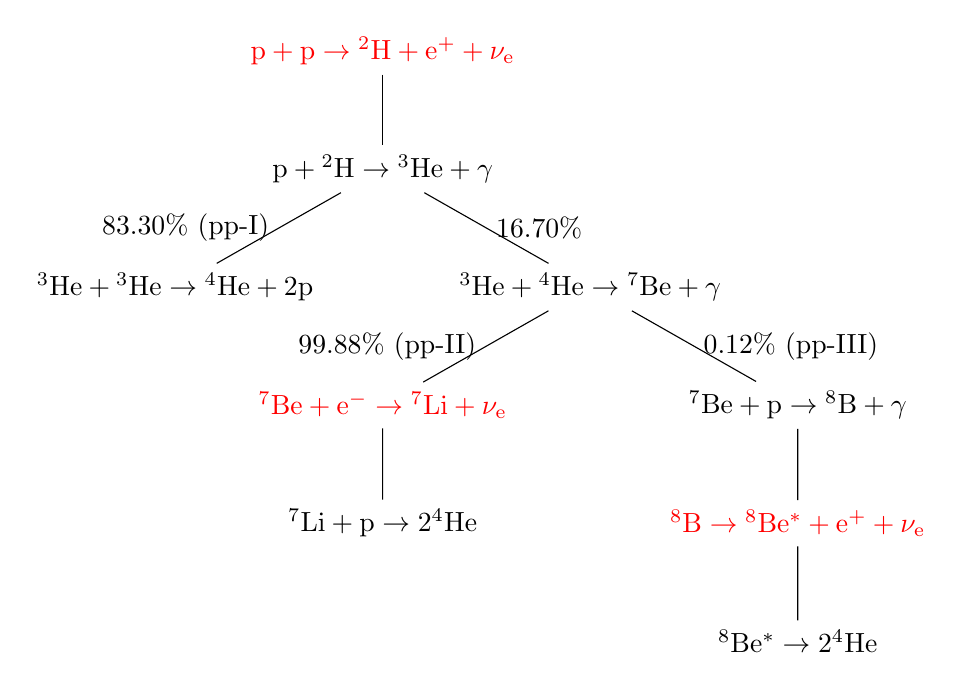
\begin{tikzpicture}[sibling distance=15em,
  every node/.style = {shape=rectangle,
    draw, align=center}
  edge from parent/.style = {draw, -latex},]]
  \node {\color{red}$\mathrm{p+p\to {}^2H + e^+ +\nu_e}$ }
    child { node {$\mathrm{p+{}^2H \to {}^3He + \gamma}$}
      child { node {$\mathrm{{}^3He+{}^3He \to {}^4 He + 2p }$}
          edge from parent node [left] {83.30\% (pp-I) } }
      child { node {$\mathrm{{}^3He+{}^4He \to {}^7 Be + \gamma }$}
        child { node {
\color{red}$\mathrm{{}^7Be + e^- \to {}^7Li + \nu_e}$
        }
        child { node { $\mathrm{{}^7Li + p \to 2{}^4He }$} }
        edge from parent node [left] {99.88\% (pp-II) } }
        child { node { $\mathrm{{}^7 Be + p \to {}^8 B + \gamma}$}
        child { node { \color{red}$\mathrm{{}^8B \to {}^8Be^* +e^+ +\nu_e}$ }
		child { node { $\mathrm{{}^8Be^* \to 2 {}^4He }$ } }}
        edge from parent node [right] {0.12\% (pp-III) } }
        edge from parent node [right] {16.70\%  } }};
\end{tikzpicture}
\end{adjustbox}
\caption{The pp chain reactions with the corresponding branching ratios. The branching ratios are taken from Ref.~\cite{Altmann2001}. }
\label{fig:pp_Chain_Branching}
\end{figure*}


% \begin{figure}[!hbtp]
% \centering
% 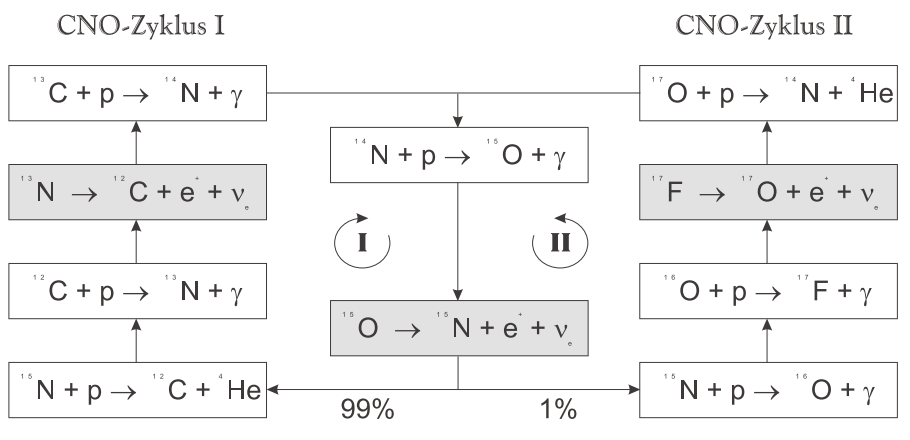
\includegraphics[width=\columnwidth]{chapters/assets/solar/cno_cycle.png}
% \caption{CNO cycle illustration~\cite{Adelberger2011a}.}
% \label{fig:cno_cycle}
% \end{figure}


Even without the knowledge of the detailed reactions, the conservation of the electric charge and the electron lepton number will lead to the overall neutrino production formula
\begin{equation}
\mathrm{4p+2e^- \to {}^4He + 2\nu_e }.
\end{equation}
It is important to notice that two neutrinos are emitted for each $\alpha$ particle, i.e., ${}^4\mathrm{He}$, produced in the Sun. Using this simple relation, we can estimate the neutrino number flux emitted by the Sun. The energy released during the production of each $\alpha$ particle is the difference between the initial and final rest masses of the particles,
\begin{equation}
Q=4m_p+2m_e-m_{\alpha}=26.7\mathrm{MeV},
\end{equation}
where the mass of the neutrinos are neglected. On average, each neutrino carries away an energy of $0.2\mathrm{MeV}$ and the rest of the energy is in the form of thermal energy $Q_\gamma=26.3\mathrm{MeV}$~\cite{Adelberger2011a}. %Energy flux density of solar photons near Earth is given by the solar constant $S_0$.
Since two neutrinos are emitted for the production of thermal energy $Q_\gamma$, the number flux of the solar neutrinos near the Earth is approximately
\begin{equation}
\Phi_\nu = \frac{2 S_0}{Q_\gamma} \approx 6\times 10^{10} \mathrm{cm^{-2}s^{-1}},
\end{equation}
where the solar constant $S_0$ is the energy flux of solar photons on the top of the Eath atmosphere.
%Neutrinos are hard to detect but a large number flux makes it possible to detect solar neutrinos~\cite{Cleveland1998,Lande2003,McDonald2013}.

% On the other hand, the solar neutrinos have a certain energy spectrum due to the composition of nuclear reactions. Inside our Sun, two additional reactions other than pp neutrinos also produce neutrinos which are called pep and hep neutrinos.
% \begin{itemize}
% \item pep neutrinos are produced in
% \begin{equation}
% \mathrm{p + e^- + p \to {}^2H +\nu_e},
% \end{equation}
% which only has a branching ratio 0.4\% instead of the 99.6\% of pp reaction.
% \item hep neutrinos are produced in
% \begin{equation}
% \mathrm{ {}^3He + p \to {}^4He + e^+ \nu_e },
% \end{equation}
% which has a branching ratio of $2\times 10^{-5}\%$. As a comparison, the $\mathrm{{}^3He + {}^3He}$ has a branching ratio $85\%$ and $\mathrm{{}^3He + {}^4He}$ has a branching ratio $15\%$.
% \end{itemize}


As the detection of neutrinos became feasible, Ray Davis and John Bahcall et al worked out the solar neutrino flux and led the Homestake experiment to measure the solar neutrinos. The results revealed that the neutrino flux detected was less than what was predicted by the standard solar model~\cite{Bahcall1973}. This is the solar neutrino problem. It is now known that the solution to the problem is related to the neutrino. The electron neutrinos produced in the solar core transform to other flavors while they travel to the Earth. This phonomenon is referred known as the flavor transformation of the neutrino, or neutrino oscillations. The theory of neutrino oscillations was first proposed by Pontecorvo in 1968~\cite{Pontecorvo1968}. The field of neutrino oscillations has grown significantly into a broad field in physics since then.



\section{Supernova Neutrinos}


Another astronomical source of neutrinos is the core-collapse supernova explosion. Massive stars with masses larger than 6−8 solar masses are very bright. However, violent delights have violent ends. When the core of a massive star runs out of nuclear fuel, it collapses under its own gravity. During the collapse, the inner core is compressed to almost nuclear density, which has a stiff equation of state. The materials falling onto the highly compressed inner core are bounced outward which generates a shock wave and may lead to an explosion. However, supernova simulations to date show that the shock wave itself is not always energetic enough to produce the explosion~\cite{Janka2016b}. In most cases, it stalls and becomes a standing accretion shock wave. To revive the shock, more energy has to be deposited behind the shock. A possible solution is to introduce reheating of the shock by neutrinos~\cite{Janka2016b}. In fact 99\% percent the energy released in a core-collapse supernova is carried away by neutrinos.
%Those explosions are the most luminous sources of neutrinos in the universe~\cite{Raffelt1996wa}.
In order to implement the neutrino-driven mechanism in computer simulations of supernovae, the flux and flavor content of the neutrinos have to be known everywhere behind the shock. Thus neutrino oscillations in dense matter become a key to the supernova explosion problem.

The average energy of the neutrinos $\langle E \rangle$ emitted during a supernova explosion is of the order of 10MeV~\cite{Janka2017}, and the neutrino luminosity at the early epoch is approximately $10^{52}\mathrm{ergs\cdot s^{-1}}$~\cite{Pejcha2012a}.
% The supernova explosion releases neutrinos with energy flux on the order of $10^{51}\mathrm{ergs\cdot s^{-1}}$~\cite{Bethe1985}.
Therefore, the number density of the neutrinos at the radius $R$ is
\begin{equation*}
   n \sim  10^{18} \mathrm{cm^{-3}} \left(\frac{100\mathrm{km}}{R}\right)^2 \left(\frac{10\mathrm{MeV}}{\langle E \rangle}\right).
\end{equation*}
% which corresponds to the number flux
% \begin{equation*}
%   \Phi \sim 10^{27} \mathrm{cm^{-2} s^{-1}}\left(\frac{100\mathrm{km}}{R}\right)^2 \left(\frac{10\mathrm{MeV}}{\langle E \rangle}\right).
% \end{equation*}
% Compared to the neutrino flux at the surface of the Sun, which is of the order $10^{15}\mathrm{cm^{-2} s^{-1}}$, supernova neutrinos is much denser.
It turns out that the ambient dense neutrino medium has a significant impact on neutrino oscillations, which has been intensely investigated in the last decade~\cite{Duan2010}.

Observation-wise, the neutrino signals from a galactic supernova can reveal a great amount of information about the physical conditions inside the supernova. In fact, the detection of supernova neutrinos is on the task list of the Deep Underground Neutrino Experiment (DUNE)~\cite{Kemp2017}.




\section{Organization of the Disseration}


% As we have seen, it is crucial to understand neutrino flavors.
The rest of the disseration is organized as follows.
In Chapter~\ref{chap:basics}, I will review neutrino oscillations in vacuum and in environments with smooth matter density profiles.
% Meanwhile, neutrino oscillations are ingredients of many other astrophysical, cosmological, and astronomical problems, such as neutron star mergers, dark matter, nucleosynthesis, etc. In order to gain a better understanding of neutrinos in these exotic environments, neutrino oscillations in dense matter background and dense neutrino background have to be thoroughly investigated. The seminal work by Mikheev--Smirnov--Wolfenstein proved neutrino interactions with matter background have significant effect on neutrino oscillations. They showed that neutrinos propagating through decreasing matter density experience a potential that alters the flavor conversions (MSW effect), which may also lead to maximum conversions between flavors~\cite{Mikheev:1986gs,wolf78,wolfensteinprd1979}. It is also know that neutrino oscillations in more general matter density profiles exhibit interesting phenomena. Resonances are found as the characteristic length scale in matter density profile and characteristic length scale of the neutrinos satisfies certain relations.
In Chapter~\ref{chap:matter}, I will discuss my work on neutrino oscillations in oscillatory matter profiles, which can be decomposed into Fourier modes and interpreted as a superposition of Rabi oscillations.
%Apart from dense matter background, neutrinos also interact with neutrinos themselves and introducing nonlinear dynamics. The neutrino self-interactions are analyzed using linear stability analysis.
In Chapter~\ref{chap:collective}, I will first review how neutrino self-interactions can cause a dense neutrino medium to oscillate collectively. Then I will discuss my study on the dispersion relations of the collective modes of neutrino oscillations.
%, as well as the dispersion relations in linear stability analysis. I will also discuss the neutrino halo problem. The halo problem exists because neutrino propagating out of dense matter medium will be scattered and forming a neutrino halo. Some of the neutrinos will propagate backward and interact with forward propagating neutrinos and alter the neutrino flavors. Mathematically speaking, the neutrino halo problem is a nonlocal boundary value problem. I will explain the numerical relaxation scheme that we developed, which we have proven to be a promising method to solve neutrino halo problem.
I will also discuss a premilinary work on neutrino oscillations when both forward and backward neutrino fluxes are present.
In Chapter~\ref{chap:conclusion}, I will summarize my work and discuss possible future directions of the field.

%!TEX root = ../phd-thesis-lei-ma.tex
%!TeX spellcheck = en-US


\chapter{\label{chap:basics}General Principles of Neutrino Oscillations}

Since the flavor eigenstates of the neutrino are not the same as its propagation eigenstates, it can change flavor while it propagates.
In this chapter, I will use the two-flavor scheme to explain neutrino oscillations in some simple scenarios.\footnote{In most physical problems, the two-flavor scheme is a good approximation to the phenomena of neutrino oscillations. The two mass splitings between the three mass eigenstates are so different that the corresponding oscillations occur on very different length scales. On a given length scale, the two-flavor scheme captures the prominent features of the neutrino oscillations of the corresponding mass spliting.}
I will first discuss neutrino oscillations in vacuum. After explaining the general principles of neutrino oscillations in matter, I will show how the solar neutrino problem can be explained by neutrino oscillations. Finally, I will demonstrate the flavor isospin picture which can be used to visualize neutrino oscillations.


\section{\label{chap:basics-sec:vacuum-oscillations}Vacuum Oscillations}

Before carrying out the calculations, I can estimate the frequency of the oscillations of the neutrino between its flavors. In the natural units, frequency has the same dimension as energy.
% (see Appendix~\ref{chap:app-sec:conventions-subsec:units}).
Consider an electron neutrino with momentum $p$ which is a superposition of the two mass eigenstates $\ket{\nu_i}$ ($i=1,2$) with masses $m_i$, respectively. Since the neutrino masses are small, I can Taylor expand the energy of each mass eigenstate in terms of the corresponding mass:
\begin{align}
E_i & = \sqrt{m_i^2 + p^2 } \nonumber\\
& = p \sqrt{\frac{m_i^2}{p^2} + 1} \nonumber\\
& \approx p + \frac{1}{2} \frac{m_i^2}{p}.
\label{chap:basics-section:neutrinos-eqn:energy-taylor}
\end{align}
The first term in the above equation produces a global phase to the flavor wave function of the neutrino which does not affect neutrino flavor oscillations. The characteristic energy scale in the problem is the difference between the energies of the two mass eigenstates,
\begin{equation}
    \omega_{\mathrm v} = E_2-E_1 =  \frac{m_2^2-m_1^2}{2E} = \frac{\delta m^2}{2E},
    \label{chap:basics-section:neutrinos-eqn:qualitative-method-frequency}
\end{equation}
which turns out to be the vacuum oscillation frequency. Here $E=p$ is approximately the energy of the neutrino.

To work out the exact solution, I will utilize the Schr\"{o}dinger equation. First of all, the flavor eigenstates are denoted as $\ket{\nu_\alpha}$ where ${}_\alpha$ can be ${}_{\mathrm{e}}$ or ${}_{\mathrm{x}}$ for the electron flavor and the other flavor. The wave function of neutrino state $\ket{\nu}$ in the flavor basis, defined as
\begin{equation}
    \Psi^{(\ff)} = \begin{pmatrix}
        \psi^{(\ff)}_{\mathrm e} \\
        \psi^{(\ff)}_{\mathrm x}
    \end{pmatrix} = \begin{pmatrix}
        \braket{\nu_{\mathrm e}}{\nu} \\
        \braket{\nu_{\mathrm x}}{\nu}
    \end{pmatrix},
\end{equation}
is related to the wave function in the vacuum mass basis $\Psi^{(\vv)}$ through a unitary mixing matrix $\mathsf U$,
\begin{equation}
\Psi^{(\mathrm f)} = \mathsf{U}\Psi^{(\vv)},
\label{chap:vacuum-eqn:wavefunction}
\end{equation}
where the upper indices ${}^{(\vv)}$ and ${}^{(\ff)}$ are used to denote the corresponding bases. The mixing matrix can be expressed using the vacuum mixing angle $\theta_{\vv}$:
\begin{equation}
\mathsf{U} = \begin{pmatrix} \cos\theta_\vv & \sin \theta_\vv \\ -\sin \theta_\vv & \cos \theta_\vv \end{pmatrix}.
\end{equation}
In the vacuum mass basis, the neutrino has a free propagation Hamiltonian
\begin{equation}
\mathsf H^{(\vv)} = \begin{pmatrix} E_1 & 0 \\
0 & E_2
\end{pmatrix}.
\end{equation}
To the first order, the Hamiltonian becomes
\begin{align}
\mathsf H^{(\vv)} &\approx \frac{1}{2E} \begin{pmatrix}
m_1^2 & 0 \\
0 & m_2^2
\end{pmatrix} + E \mathsf{I} \nonumber \\
& =  \frac{1}{4E} \begin{pmatrix}
 - \delta m^2 & 0 \\
0 & \delta m^2
\end{pmatrix}  + \left(\frac{m_2^2 + m_1^2}{4E}  + E \right) \mathsf{I}.
\end{align}
Because a multiple of the identity matrix $\mathsf{I}$ gives only a global phase to the neutrino flavor wave function, I will neglect it from now on, and the vacuum Hamiltonian simplifies to
\begin{equation}
\mathsf H^{(\vv)} \to  \frac{\delta m^2}{4E} \begin{pmatrix}
-1 & 0 \\
0 & 1
\end{pmatrix} = -\frac{\delta m^2}{4E} \sigma_3 = -\frac{\omega_{\vv}}{2}\sigma_3,
\end{equation}
where
\begin{align}
\sigma_1 &=  \begin{pmatrix}
0 & 1 \\
1 & 0
\end{pmatrix}, &\sigma_2 &=  \begin{pmatrix}
0 & -\ii \\
\ii & 0
\end{pmatrix},  &\sigma_3 &=  \begin{pmatrix}
1 & 0 \\
0 & -1
\end{pmatrix}
\end{align}
are the three Pauli matrices.
The Schr\"{o}dinger equation has the following simple solution in the mass basis:
\begin{equation}
\Psi^{(\vv)}(t) = \begin{pmatrix}
c_1(0) e^{i \omega_\vv t/2 } \\
c_2(0) e^{ -i\omega_\vv t/2 }
\end{pmatrix}.
\end{equation}
% where the initial condition is
% \begin{equation}
% \Psi_v^{(v)}(0) = \begin{pmatrix}
% c_1(0) \\
% c_2(0)
% \end{pmatrix}.
% \end{equation}
Using Eqn.~\eqref{chap:vacuum-eqn:wavefunction}, I obtain the wave function in the flavor basis,
\begin{align}
\Psi^{(\ff)}(t) &= \mathsf{U}\Psi^{(\vv)}(t) \\
& = \begin{pmatrix} \cos\theta_\vv & \sin \theta_\vv \\ -\sin \theta_\vv & \cos \theta_\vv \end{pmatrix} \begin{pmatrix} c_1(0) e^{i\omega_\vv t/2 } \\
c_2(0) e^{ -i\omega_\vv t/2 }    \end{pmatrix} .
\label{chap:vacuum-eqn:wavefuncion-time}
\end{align}
Alternatively, I can also determine the Hamiltonian in the flavor basis first, which is
%then solve the Sch\"{o}dinger equation. I will not show the steps here, however, the Hamiltonian in flavor basis is presented for future use,
\begin{equation}
\mathsf H^{(\ff)} = \mathsf U \mathsf H^{(\vv)} \mathsf U^\dagger = -\frac{\omega_\vv}{2}\cos 2\theta_\vv \sigma_3 + \frac{\omega_\vv}{2} \sin 2\theta_\vv \sigma_1.
    \label{chap:basics-sec:vacuum-osc-eqn:hamiltonian-vacuum}
\end{equation}
By solving the Schr\"{o}dinger equation in the flavor basis, I will obtain the same wave function as in Eqn.~\eqref{chap:vacuum-eqn:wavefuncion-time}.

%In many astrophysical neutrino sources such as the solar core, electron neutrinos are the most abundant. Thus the initial condition is usually assumed to be electron flavor in the calculation which leads to the survival probability of electron flavor
The probability for a neutrino emitted in the electron flavor at time $t=0$ to be detected as the electron flavor at a later time $t$ is
\begin{equation}
P(t) = 1-\sin^2(2\theta_\vv)\sin^2\left( \frac{\omega_\vv t}{2} \right).
\end{equation}
Since the neutrino travels with approximately the speed of light, the electron neutrino survival probability at a distance $r$ from the source is
\begin{equation}
P(r) =  1-\sin^2(2\theta_\vv)\sin^2\left( \frac{\omega_\vv}{2} r \right).
\label{chap:basics-eqn:vacuum-electron-probability}
\end{equation}
%An important parameter in vacuum oscillations is the oscillation length of the neutrino flavor conversion which is $1/\omega_\vv$.This confirms our qualitative method result in Eqn.~\eqref{chap:basics-section:neutrinos-eqn:qualitative-method-frequency}.
I plot the above result in Fig.~\ref{chap:basics-section:neutrinos-fig:vacuum-2-flavor-osc} which clearly shows the oscillatory behavior. The oscillation length is determined by the characteristic energy scale $\omega_\vv$, which confirms our estimation in Eqn.~\eqref{chap:basics-section:neutrinos-eqn:qualitative-method-frequency}. The oscillation amplitude is determined by $\sin^2(2\theta_\vv)$.

\begin{figure}[htp]
    \centering
    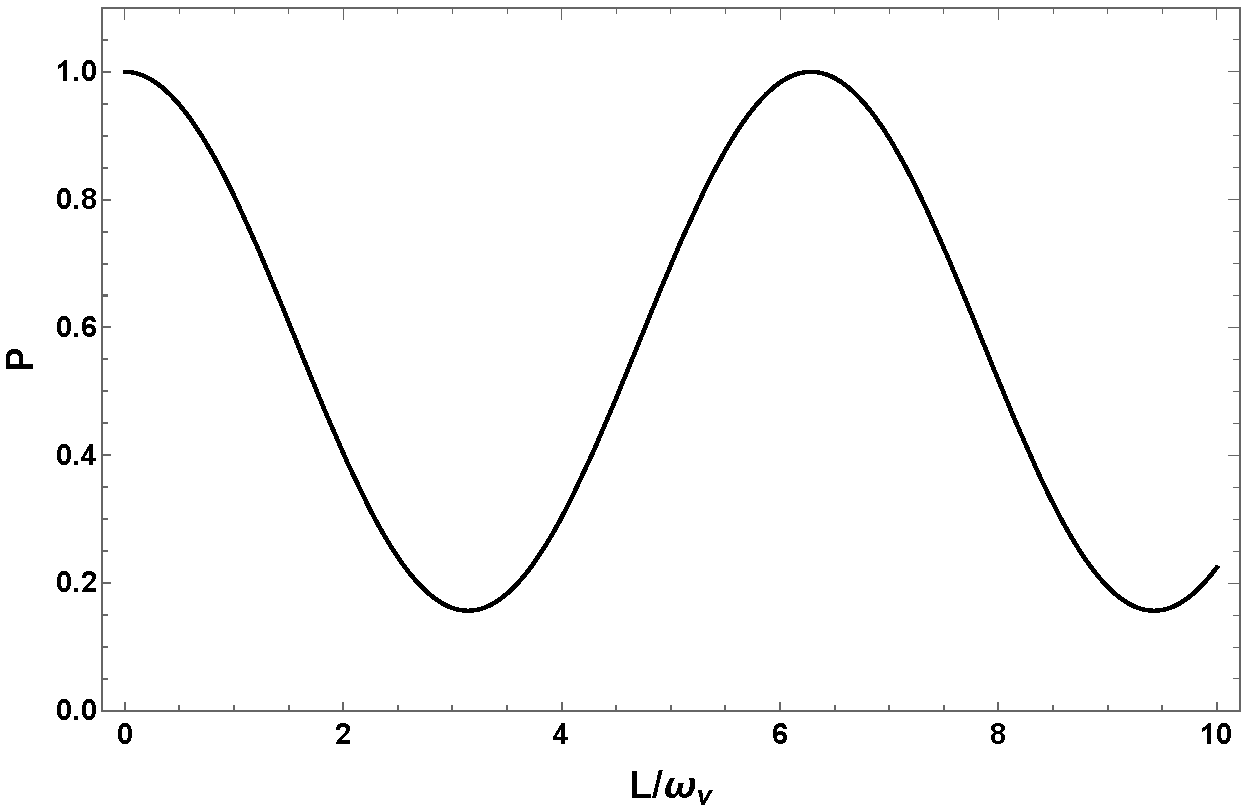
\includegraphics[width=0.8\textwidth]{chapters/assets/basics/neutrino-vaccum-osc-2-flavor.pdf}
    \caption{The electron flavor neutrino survival probability in vacuum oscillations as a function of distance $r$ which is measured in terms of vacuum oscillation frequency $\omega_\vv$. The mixing angle $\theta_\vv$ is given by $\sin^2\theta_\vv=0.30 \approx \sin^2 \theta_{12}$.}
    \label{chap:basics-section:neutrinos-fig:vacuum-2-flavor-osc}
\end{figure}



\begin{figure}[htp]
	\centering
	\begin{subfigure}[t]{0.48\textwidth}
		\centering
		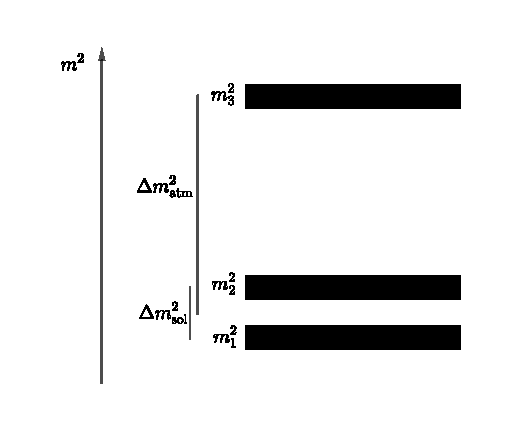
\includegraphics[width=\textwidth]{chapters/assets/basics/masses-nh}
		\caption{Normal hierarchy: the third mass is heavier than the first two.}
    \label{chap:basics-sec:flavor-isospin-pic-fig:masses-nh}
	\end{subfigure}
	\quad
	\begin{subfigure}[t]{0.48\textwidth}
		\centering
		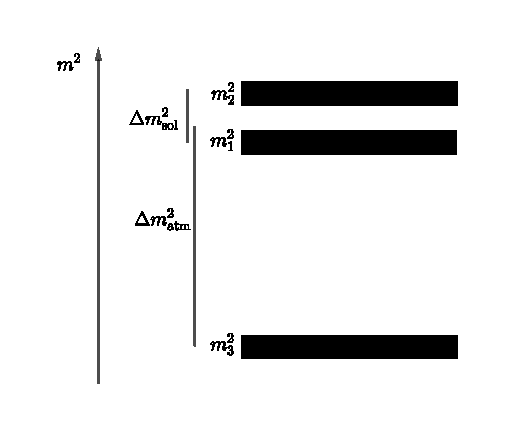
\includegraphics[width=\textwidth]{chapters/assets/basics/masses-ih}
		\caption{Inverted hierarchy: the third mass is smaller than the first two.}
    \label{chap:basics-sec:flavor-isospin-pic-fig:masses-ih}
	\end{subfigure}
	\caption{The order of the three neutrino masses. The difference between the first two masses is responsible for solar neutrino oscillations, and the difference between the third mass and the first two is responsible for atmospheric neutrino oscillations.}
    \label{chap:basics-sec:flavor-isospin-pic-fig:masses}
\end{figure}

\begin{figure}[htbp]
    \centering
    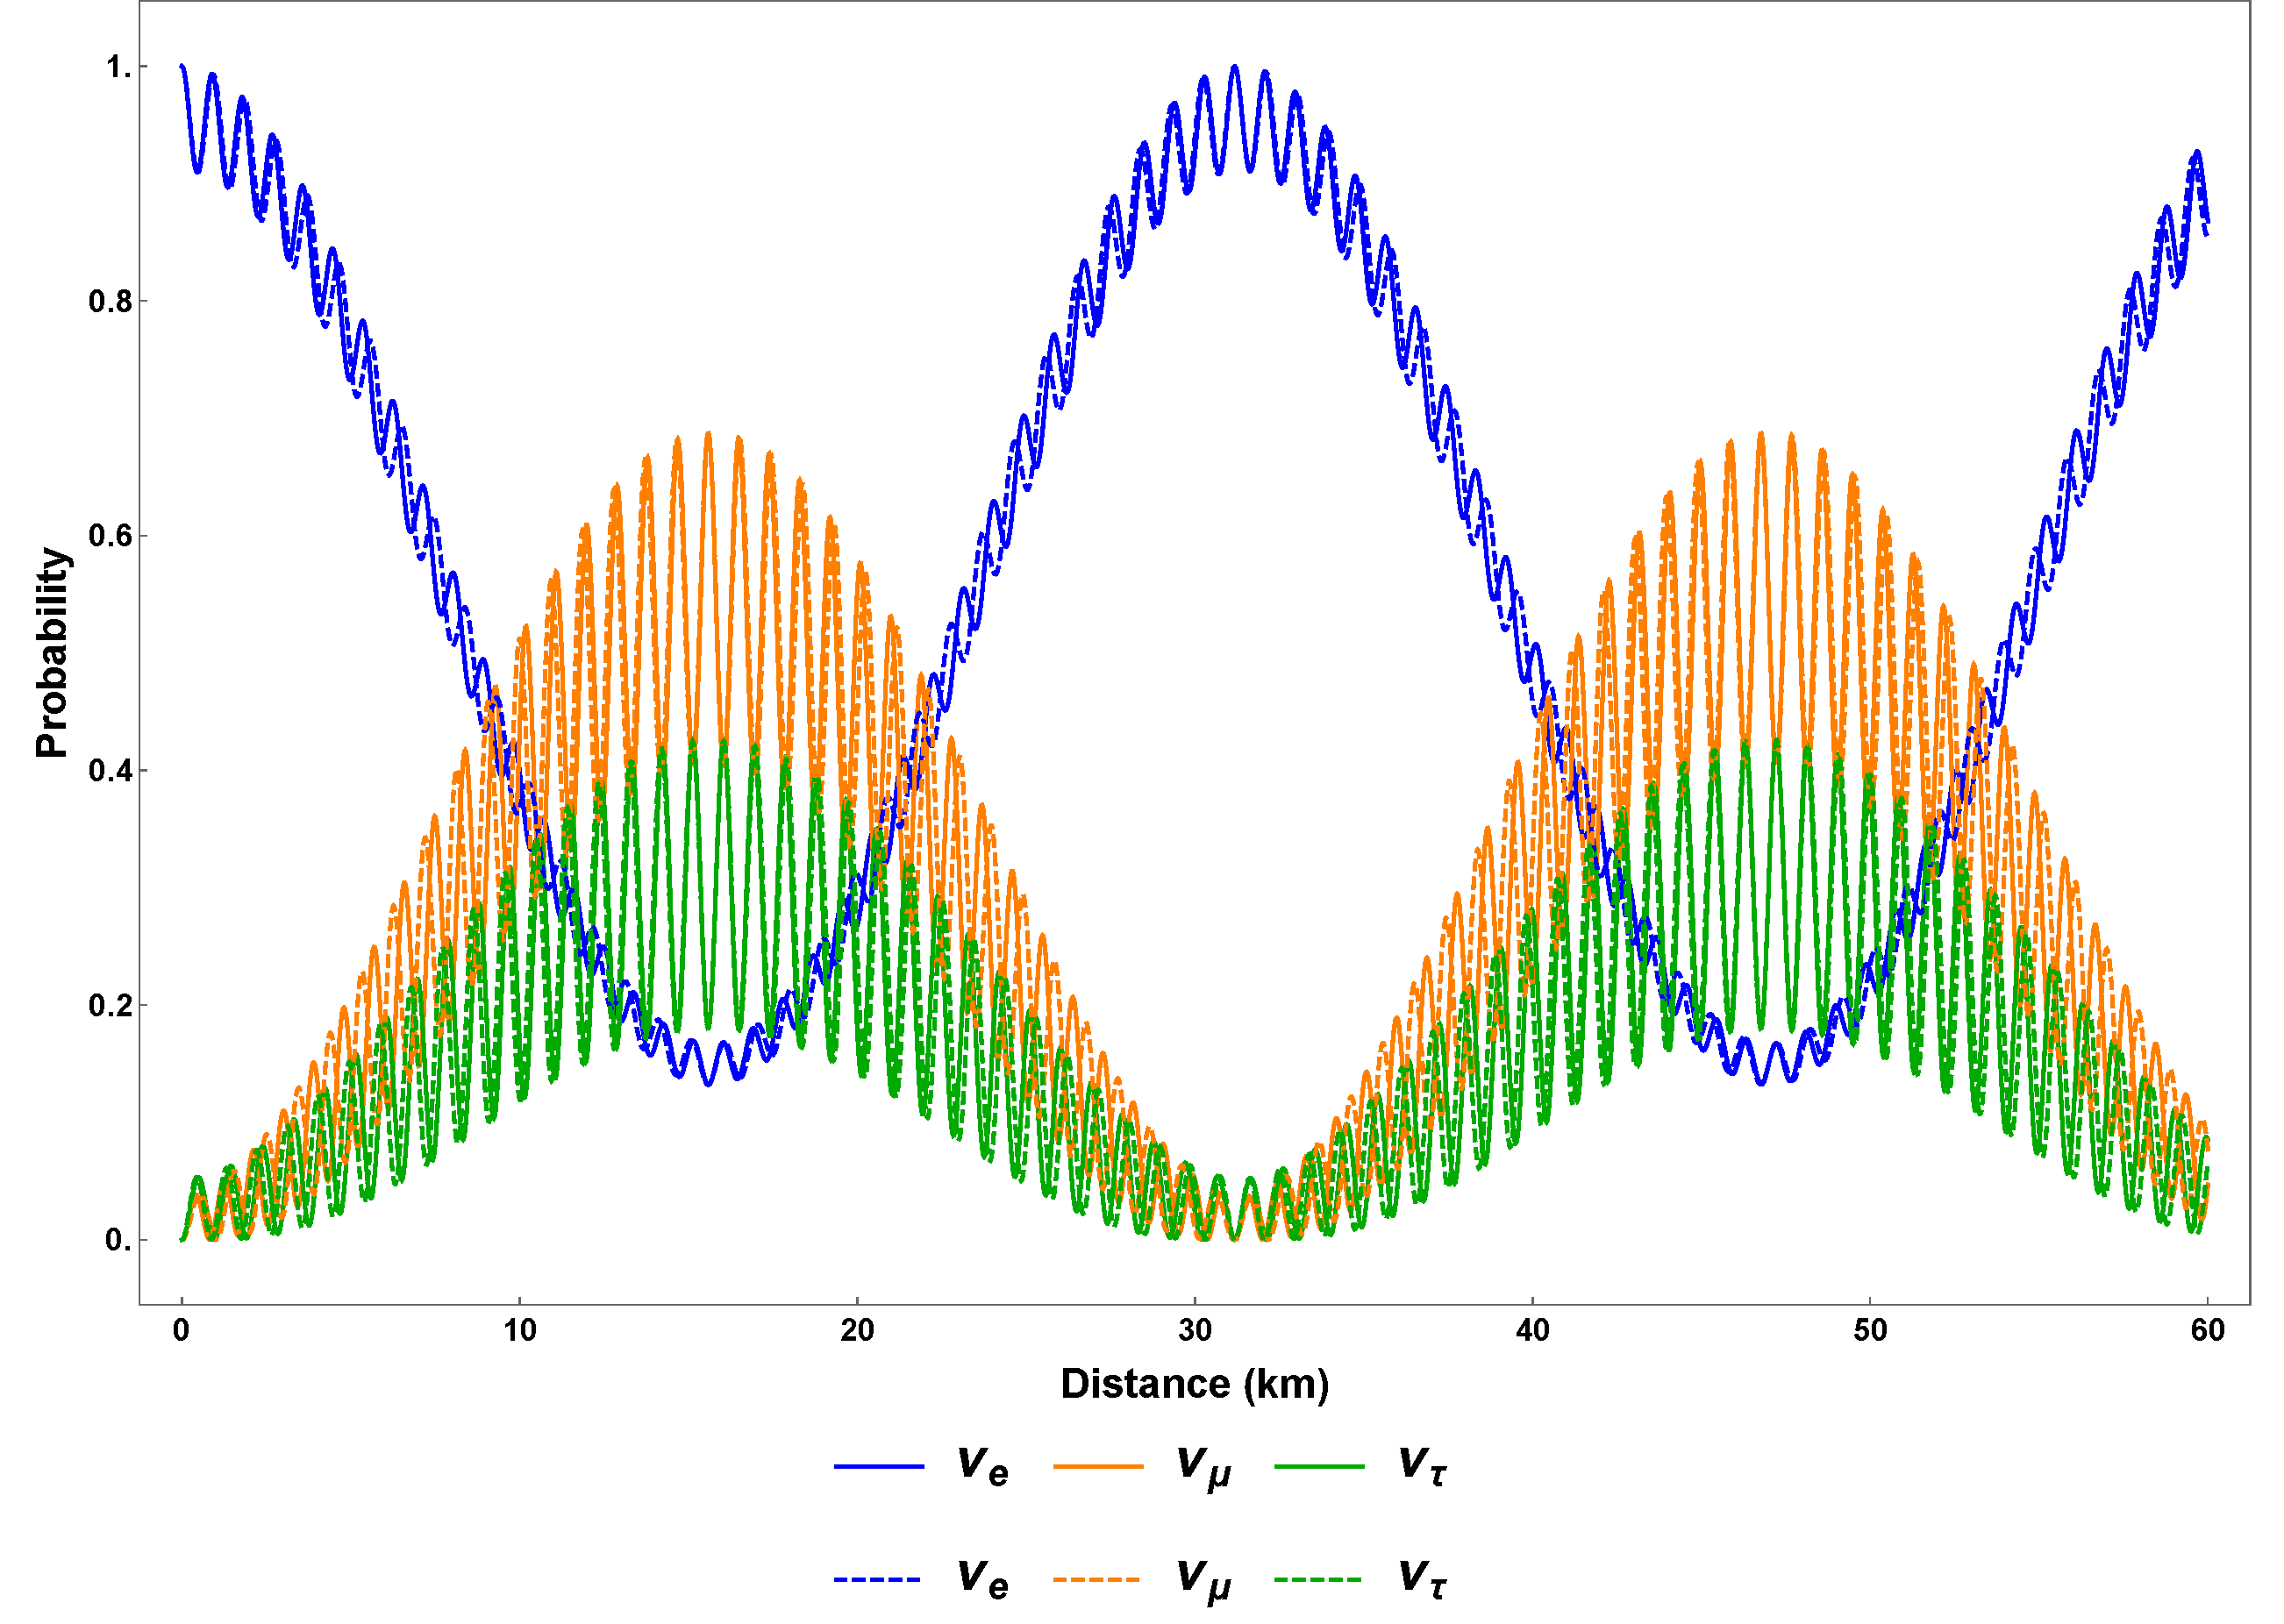
\includegraphics[width=\textwidth]{chapters/assets/basics/vacuum-oscillations-3-flavor.pdf}
    \caption{The probabilities for a $1\mathrm{MeV}$ neutrino, which is in the electron flavor initially, in different flavors as functions of the distance in vacuum. The solid lines represent the normal hierarchy and the dashed lines represent the inverted hierarchy. The mixing angles are $\sin^2\theta_{12}=0.30$, $\sin^2\theta_{13}=0.023$, and $\sin^2\theta_{23}=0.41$, respectively, and the mass differences are $\delta m_{21}^2 = 7.9\times 10^{-5}\mathrm{eV^2}$ and $\delta m^2_{23}=2.7\times 10^{-3}\mathrm{eV^2}$.}
    \label{chap:basics-section:neutrinos-fig:vacuum-3-flavor-osc}
\end{figure}


In nature, there are three neutrino flavors and, correspondingly, three neutrino mass eigenstates as shown in Fig.~\ref{chap:basics-sec:flavor-isospin-pic-fig:masses}. Because there are two different characteristic energy scales, $\omega_{\vv,21}=\delta m_{21}^2/2E$ and $\omega_{\vv,32}=\delta m_{31}^2/2E$, two oscillation periods should occur, as shown in Fig.~\ref{chap:basics-section:neutrinos-fig:vacuum-3-flavor-osc}. The fast oscillations are determined by the larger energy scale, $\omega_{\vv,32}$, while the slow oscillations are determined by the smaller one $\omega_{\vv,21}$. For the inverted neutrino mass hierarchy (with $m_3 < m_1 < m_2$), the oscillation frequencies are the same as in the normal mass hierarchy (with $m_3>m_2>m_1$) since they have the same characteristic energy scales. However, they will develop different phases during oscillations.

\clearpage

\section{\label{chap:basics-sec:oscillations-matter}Neutrino Oscillations in Matter}

\begin{figure}[htbp]
\centering
	\begin{subfigure}[t]{0.40\textwidth}
		\centering
		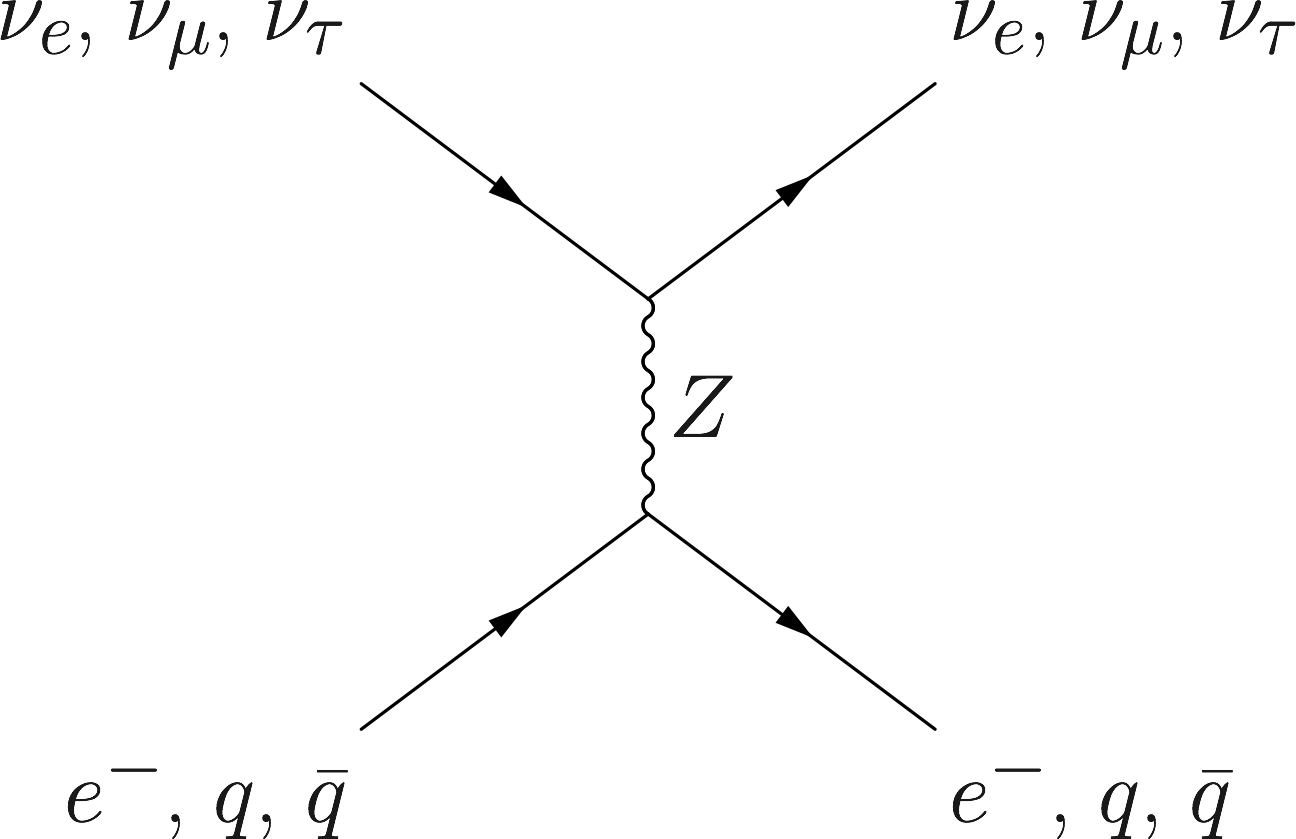
\includegraphics[height=0.2\textheight]{chapters/assets/matter/neutral-current.png}
    \caption{  }
		% \caption{Neutral current interaction between $\nu_{\mathrm e}$, $\nu_{\mu}$, $\nu_{\tau}$, and $e^{-}$. Neutral current interaction is mediated by Z bosons.}
    \label{chap:matter-fig:nc}
	\end{subfigure}%
  \qquad
	\begin{subfigure}[t]{0.40\textwidth}
		\centering
		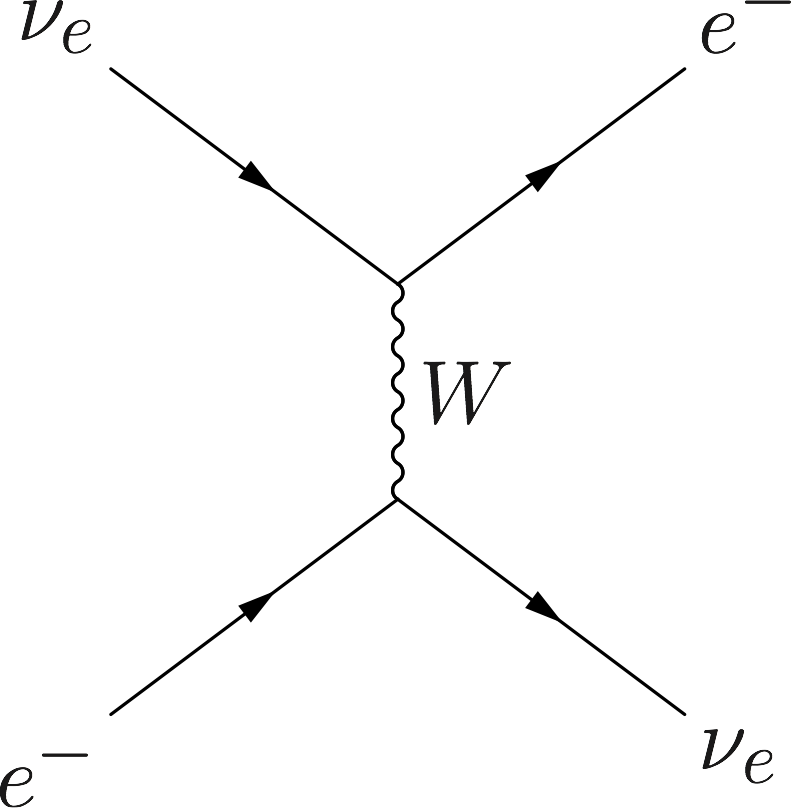
\includegraphics[height=0.2\textheight]{chapters/assets/matter/charged-current.png}
    \caption{  }
		% \caption{charged current interaction between $\nu_{\mathrm e}$ and $e^{-}$. Charged current interaction is mediated by W bosons.}
    \label{chap:matter-fig:cc}
	\end{subfigure}
	\caption{
  (a) The neutral current weak interaction does not distinguish between neutrino flavors and has no impact on neutrino oscillations. (b) The electron flavor neutrino acquires a unique refractive index contribution from the charged current weak interaction with ambient electrons.
  }
    \label{chap:matter-fig:nc-cc}
\end{figure}

In many astrophysical environments such as stars and core-collapse supernovae, neutrinos are mostly produced at the center of the environments and propagate through the dense matter envelope. Although this matter envelope is essentially transparent to neutrinos, the refractive indices of the neutrinos in matter are different than those in vacuum.\footnote{The word ``matter" in this dissertation refers to ordinary matter composed of electrons, positrons, nucleons and nuclei. I assume that the temperature and density of the environment are not high enough to produce muons and tau particles. I will discuss the effect of the dense neutrino medium in Chapter~\ref{chap:collective}.} Because the neutral current weak interaction does not distinguish between neutrino flavors (see Fig.~\ref{chap:matter-fig:nc}), it has no impact on neutrino oscillations, and I will ignore it from now on. Meanwhile, the electrons and positrons in matter will cause electron flavor neutrinos to have refractive indices different than the neutrinos of other flavors through the charged current weak interaction (see Fig.~\ref{chap:matter-fig:cc}).
% One of the significant matter effect on neutrino flavor oscillations is the Mikheyev-Smirnov-Wolfenstein (MSW) effect~\cite{Mikheev:1986gs,wolf78,wolfensteinprd1979}, which is used to explain the deficit of electron flavor neutrino flux, as know as the solar neutrino problem~\cite{kuo1989,Petcov2002}. Later developments on the theories of matter effect revealed the parametric resonance of neutrino flavor oscillations due to fluctuations in matter density~\cite{Krastev1989,Akhmedov2000}, which is the neutrino analog of transitions between energy levels as a result of external optical stimulation. Parametric resonance is different from the MSW effect since it involves the parameters of the matter density, which is usually the period of matter density fluctuations. It has also be shown that neutrinos passing through the Earth can experience parametric resonance~\cite{Akhmedov1999, Petcov1998b}.
%Flavor conversion occurs as long as their propagation eigenstates are different from their flavor eigenstates. Since the neutral current interactions between the neutrinos and the matter is independent of the flavors, as shown in Fig.~\ref{chap:matter-fig:nc}, I only include the charged current interactions in the Hamiltonian, which is an effective potential for electron flavor.
This leads to an effective potential
\begin{equation}
\mathsf V^{(\ff)} = \frac{\sqrt{2}G_{\mathrm F} n_{\mathrm e} }{2}  \sigma_3,
\label{chap:basics-sec:oscillations-matter-eqn:effective-pot}
\end{equation}
where $G_{\mathrm F}=1.17\times 10^{-5}\mathrm{GeV^{-2}}$ is Fermi constant and $n_{\mathrm e}$ is net number density of the electron. As usual, I have ignored the trace terms in the above expression.

The Hamiltonian with the matter effect is the combination of Eqn.~\eqref{chap:basics-sec:vacuum-osc-eqn:hamiltonian-vacuum} and Eqn.~\eqref{chap:basics-sec:oscillations-matter-eqn:effective-pot}:
% \begin{equation}
% \mathsf H^{(\ff)} = \frac{ \omega_\vv }{2}\begin{pmatrix} -\cos 2\theta_\vv & \sin 2 \theta_\vv \\ \sin 2\theta_\vv & \cos 2\theta_\vv  \end{pmatrix},
% \end{equation}
% where we used the result of flavor basis vacuum oscillation Hamiltonian
% \begin{align}
% \mathsf H_\vv^{(\ff)}& = \mathsf{U} \mathsf H_\vv \mathsf{U}^\dagger \\
% &= \frac{ \omega_\vv }{2}\begin{pmatrix} -\cos 2\theta_\vv & \sin 2 \theta_\vv \\ \sin 2\theta_\vv & \cos 2\theta_\vv  \end{pmatrix}.
% \end{align}
\begin{equation}
\mathsf H^{(\ff)} = \left(\frac{\lambda}{2} -\frac{ \omega_\vv }{2} \cos 2\theta_\vv \right) {\sigma}_3  + \frac{ \omega_\vv }{2} \sin 2\theta_\vv {\sigma}_1,
\label{chap:basics-sec:msw-eqn:hamiltonian-matter-effect}
\end{equation}
where
\begin{equation}
  \lambda = \sqrt{2}G_{\mathrm F} n_{\mathrm e}.
  \label{chap:basics-sec:oscillations-matter-eqn:lambda}
\end{equation}
Due to the off-diagonal terms in $\mathsf H^{(\ff)}$, the neutrino will experience oscillations in flavor. A resonance with the maximum flavor mixing occurs when the diagonal terms of $\mathsf H^{(\ff)}$ vanish, i.e.,
\begin{equation}
\frac{\lambda}{2} -\frac{ \omega }{2} \cos 2\theta_\vv  = 0,
\label{chap:basics-eqn:msw-resonance}
\end{equation}
which gives the Mikheyev--Smirnov--Wolfenstein (MSW) resonance condition.


\section{\label{chap:matter-sec:solar-neutrinos}Neutrino Oscillations in the Sun}


% \section{\label{chap:basics-sec:msw}Mikheyev--Smirnov--Wolfenstein Effect}

The neutrinos produced in the solar core experience decreasing matter density as they travel outward through the Sun. The neutrino propagation eigenstates are different from the flavor states in general~\cite{wolf78}.
%The importance of matter effect to our understanding of solar neutrinos is that it modifies the oscillations, depending on the matter density variation.
Because the density change inside the Sun is not dramatic, the flavor quantum states of the neutrinos will evolve adiabatically inside the Sun.

\begin{figure}[htbp]
\centering
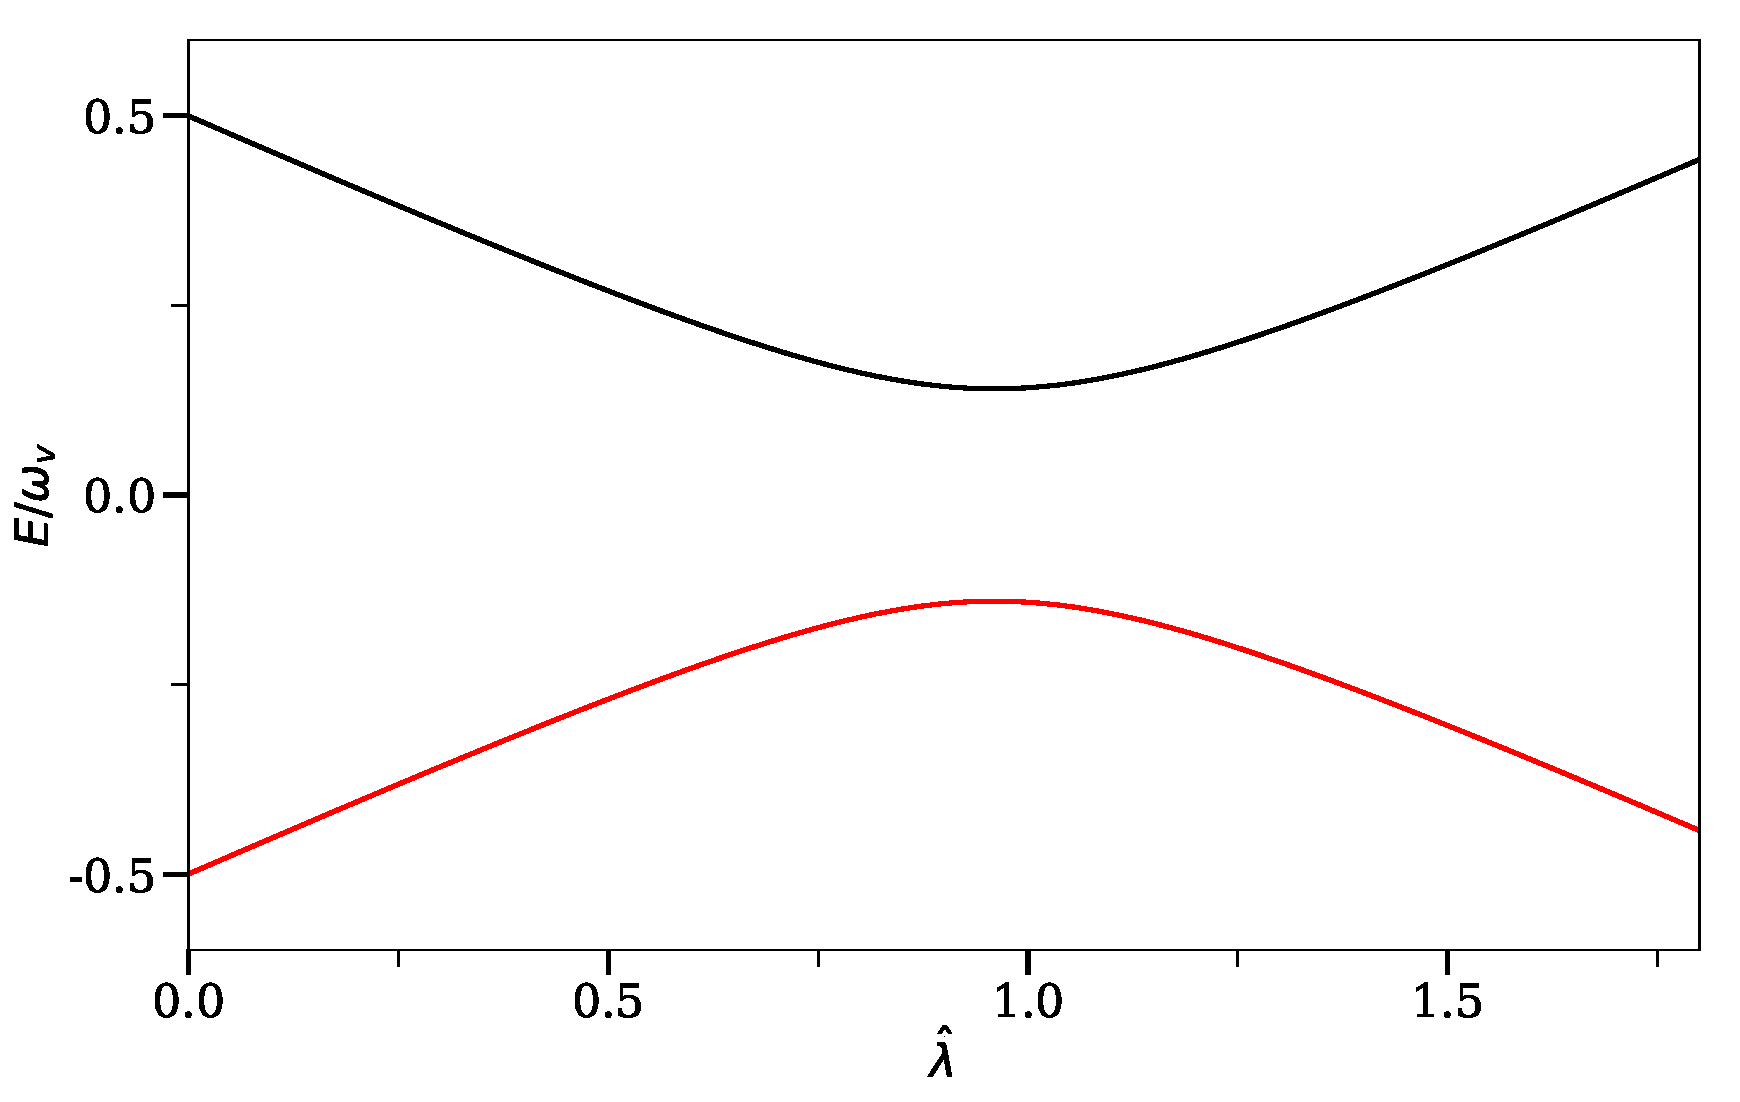
\includegraphics[width=0.7\columnwidth]{chapters/assets/matter/mswEnergyLevels}
\caption{The two eigenvalues of the neutrino Hamiltonian as functions of matter potential $\hat\lambda$. I have used $\sin^2\theta_\vv = 0.02 \approx \sin^2 \theta_{13}$.}
\label{fig:mswEnergyLevels}
\end{figure}

The values of the instantaneous eigenstates of the Hamiltonian, known as the ``Heavy'' and ``Light'' states, are
\begin{align}
\varepsilon_{\mathrm H} &= \frac{\omega_\vv}{2}\sqrt{ \hat\lambda +1 -  2\hat\lambda \cos 2\theta_\vv }, \\
\varepsilon_{\mathrm L} &= -\frac{\omega_\vv}{2}\sqrt{ \hat\lambda +1 -  2\hat\lambda \cos 2\theta_\vv },
\end{align}
% which means that the instantaneous eigenstates and eigenvectors of Hamiltonian is good enough for the time dependent Schr\"{o}dinger equation.
where
\begin{align}
\hat\lambda & = \frac{\lambda}{\omega_\vv}.
\end{align}
In Fig.~\ref{fig:mswEnergyLevels}, I show the two eigenvalues of the neutrino Hamiltonian as functions of the matter potential $\hat \lambda$.

For a very high matter density, the heavy state of the neutrino $\ket{\nu_{\mathrm H}}$ is almost the same as $\ket{\nu_{\ee}}$. As the matter density decreases, $\ket{\nu_{\mathrm H}}$ becomes a mixture of different neutrino flavors. As the neutrino reaches the surface of the Sun, where the matter density is approximately zero, $\ket{\nu_{\mathrm H}}$ is about the same as vacuum mass eigenstate $\ket{\nu_{2}}$. As a result, the electron flavor neutrinos produced at the solar core are partially converted to other flavors as they reach the surface of the Sun. This explains the solar neutrino problem.
% The MSW resonance occurs at $n_{\mathrm e} = 2\omega_\vv \cos(2\theta_\vv)/\sqrt{2}G_{\mathrm F}$.
%Neutrinos with different energies will encounter the MSW resonance at different matter densities, which will significantly reshape the neutrino energy spectra.
% Even though only the electron flavor neutrinos are produced in the Sun, the neutrino flavor conversion to the other flavors is enhanced by the matter interactions, in addition to the vacuum oscillation.
%The exact neutrino flavor conversion is much more complicated than the MSW effect.
% As an approximation, the MSW transition is good enough for the solar neutrinos flavor oscillations~\cite{Lopes2013a}.

% One of the interesting fact about MSW effect is the MSW triangle shown in Fig.~\ref{chap:basics-sec:msw-fig:msw-triangle}. The survival probability of the electron flavor neutrinos is plotted against $\log (\lambda/\omega_\vv)$ and $\log (\sin^2 2\theta_\vv)$. Qualitatively speaking, large conversion happens when matter density is not too small since a sufficient central potential is required for the level crossing. This leads to the triangle shape of the low survival probability region.
%
% \begin{figure}[htbp]
%     \centering
%     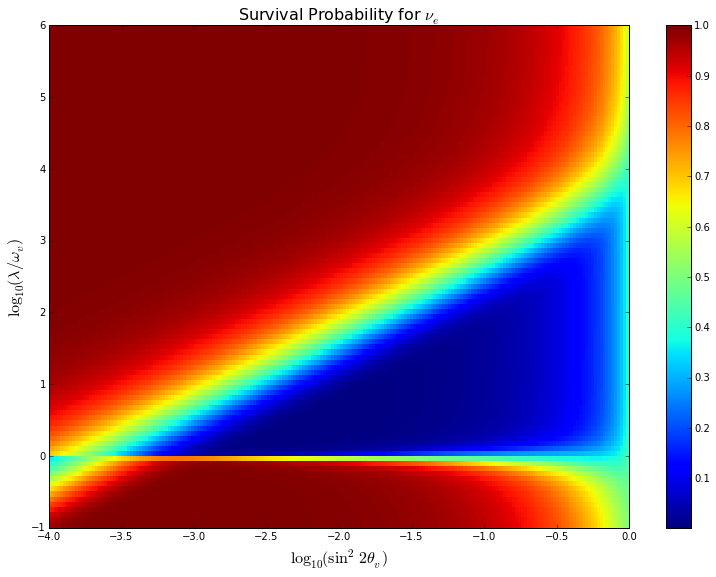
\includegraphics[width=0.9\textwidth]{chapters/assets/basics/msw-triangle.png}
%     \caption{MSW triangle. The horizontal axis is related to the the mixing angles, and the vertical axis is related to the matter potential in the center of the Sun. The colors are the survival probabilities of electron flavor. The region of large conversions, or small survival probabilities, forms a triangle. The larger the mixing angle, the larger range of matter potential for large conversions.}
%     \label{chap:basics-sec:msw-fig:msw-triangle}
% \end{figure}





% \section{\label{chap:matter-sec:flavor-isospin}Flavor Isospin Formalism}













\section{\label{chap:basics-sec:flavor-isospin-pic}Flavor Isospin Formalism}


\begin{figure}
    \centering
    \vspace*{-10pt}
    \includegraphics[width=\textwidth]{chapters/assets/basics/flavor-isospin-illus}
    \caption{In the flavor isospin picture, a flavor isospin pointing upward, i.e., along the third axis in flavor space, indicates that the neutrino is in the electron flavor, while the downward direction indicates the other flavor, such as the muon flavor.}
    \label{chap:basics-sec:flavor-isospin-pic-fig:flavor-isospin-illus}
\end{figure}

The Hamiltonian for two-flavor neutrino oscillations describes a two-level quantum system. It is known that two-level quantum systems can be visualized using the Bloch sphere. In the realm of neutrino physics, the neutrino flavor isospin was introduced for such purpose~\cite{Duan2006b}.


Every two-by-two Hermitian matrix can be expanded in the quaternion basis. For example, the Hamiltonian for neutrino oscillations in vacuum (in the flavor basis) can be written as
\begin{equation}
\mathsf H^{(\ff)} = - \frac{\vec{\sigma} }{2}\cdot {\vec{H}},
\end{equation}
where
\begin{align}
{\vec H} =  \omega_\vv\begin{pmatrix}
 \sin \theta_\vv\\
0\\
\cos 2\theta_{\mathrm v}
\end{pmatrix},
\end{align}
which is a vector of length $\omega_{\mathrm v}$ and tilted away from the third axis by angle $2\theta_{\mathrm v}$.
Throughout the dissertation, I will use ``$\vec{\phantom{x~}}$" to denote a vector in flavor space.
The flavor quantum state of the neutrino is represented by its flavor isospin which is defined as
\begin{equation}
    \vec s = {\Psi^{(\ff)}}^{\dagger} \frac{\vec{\sigma} }{2} \Psi^{(\ff)}.
\end{equation}
As shown in Fig.~\ref{chap:basics-sec:flavor-isospin-pic-fig:flavor-isospin-illus}, the direction of the flavor isospin in flavor space shows the flavor content of the neutrino. A flavor isospin pointing ``upward'' in flavor space, i.e., along the direction of the third axis, denotes the electron flavor by definition.
Correspondingly, the equation of motion for the flavor isospin describes its precession around the vector $\vec{H}$,
\begin{equation}
\dot{\vec{s}} = {\vec{s}} \times \vec{H},
\label{chap:basics-sec:flavor-isospin-pic-eqn:eom-precession}
\end{equation}
where $\dot{\phantom{s}}$ indicates the time derivative.
In the flavor isospin formalism, the electron flavor survival probability is
\begin{equation}
P = \frac{1}{2} + s_3,
\label{chap:basics-sec:flavor-isospin-pic-eqn:probability-flavor}
\end{equation}
where $s_3$ is the third component of the flavor isospin.
\begin{figure}[htbp]
    \centering
    % \vspace*{-20pt}
    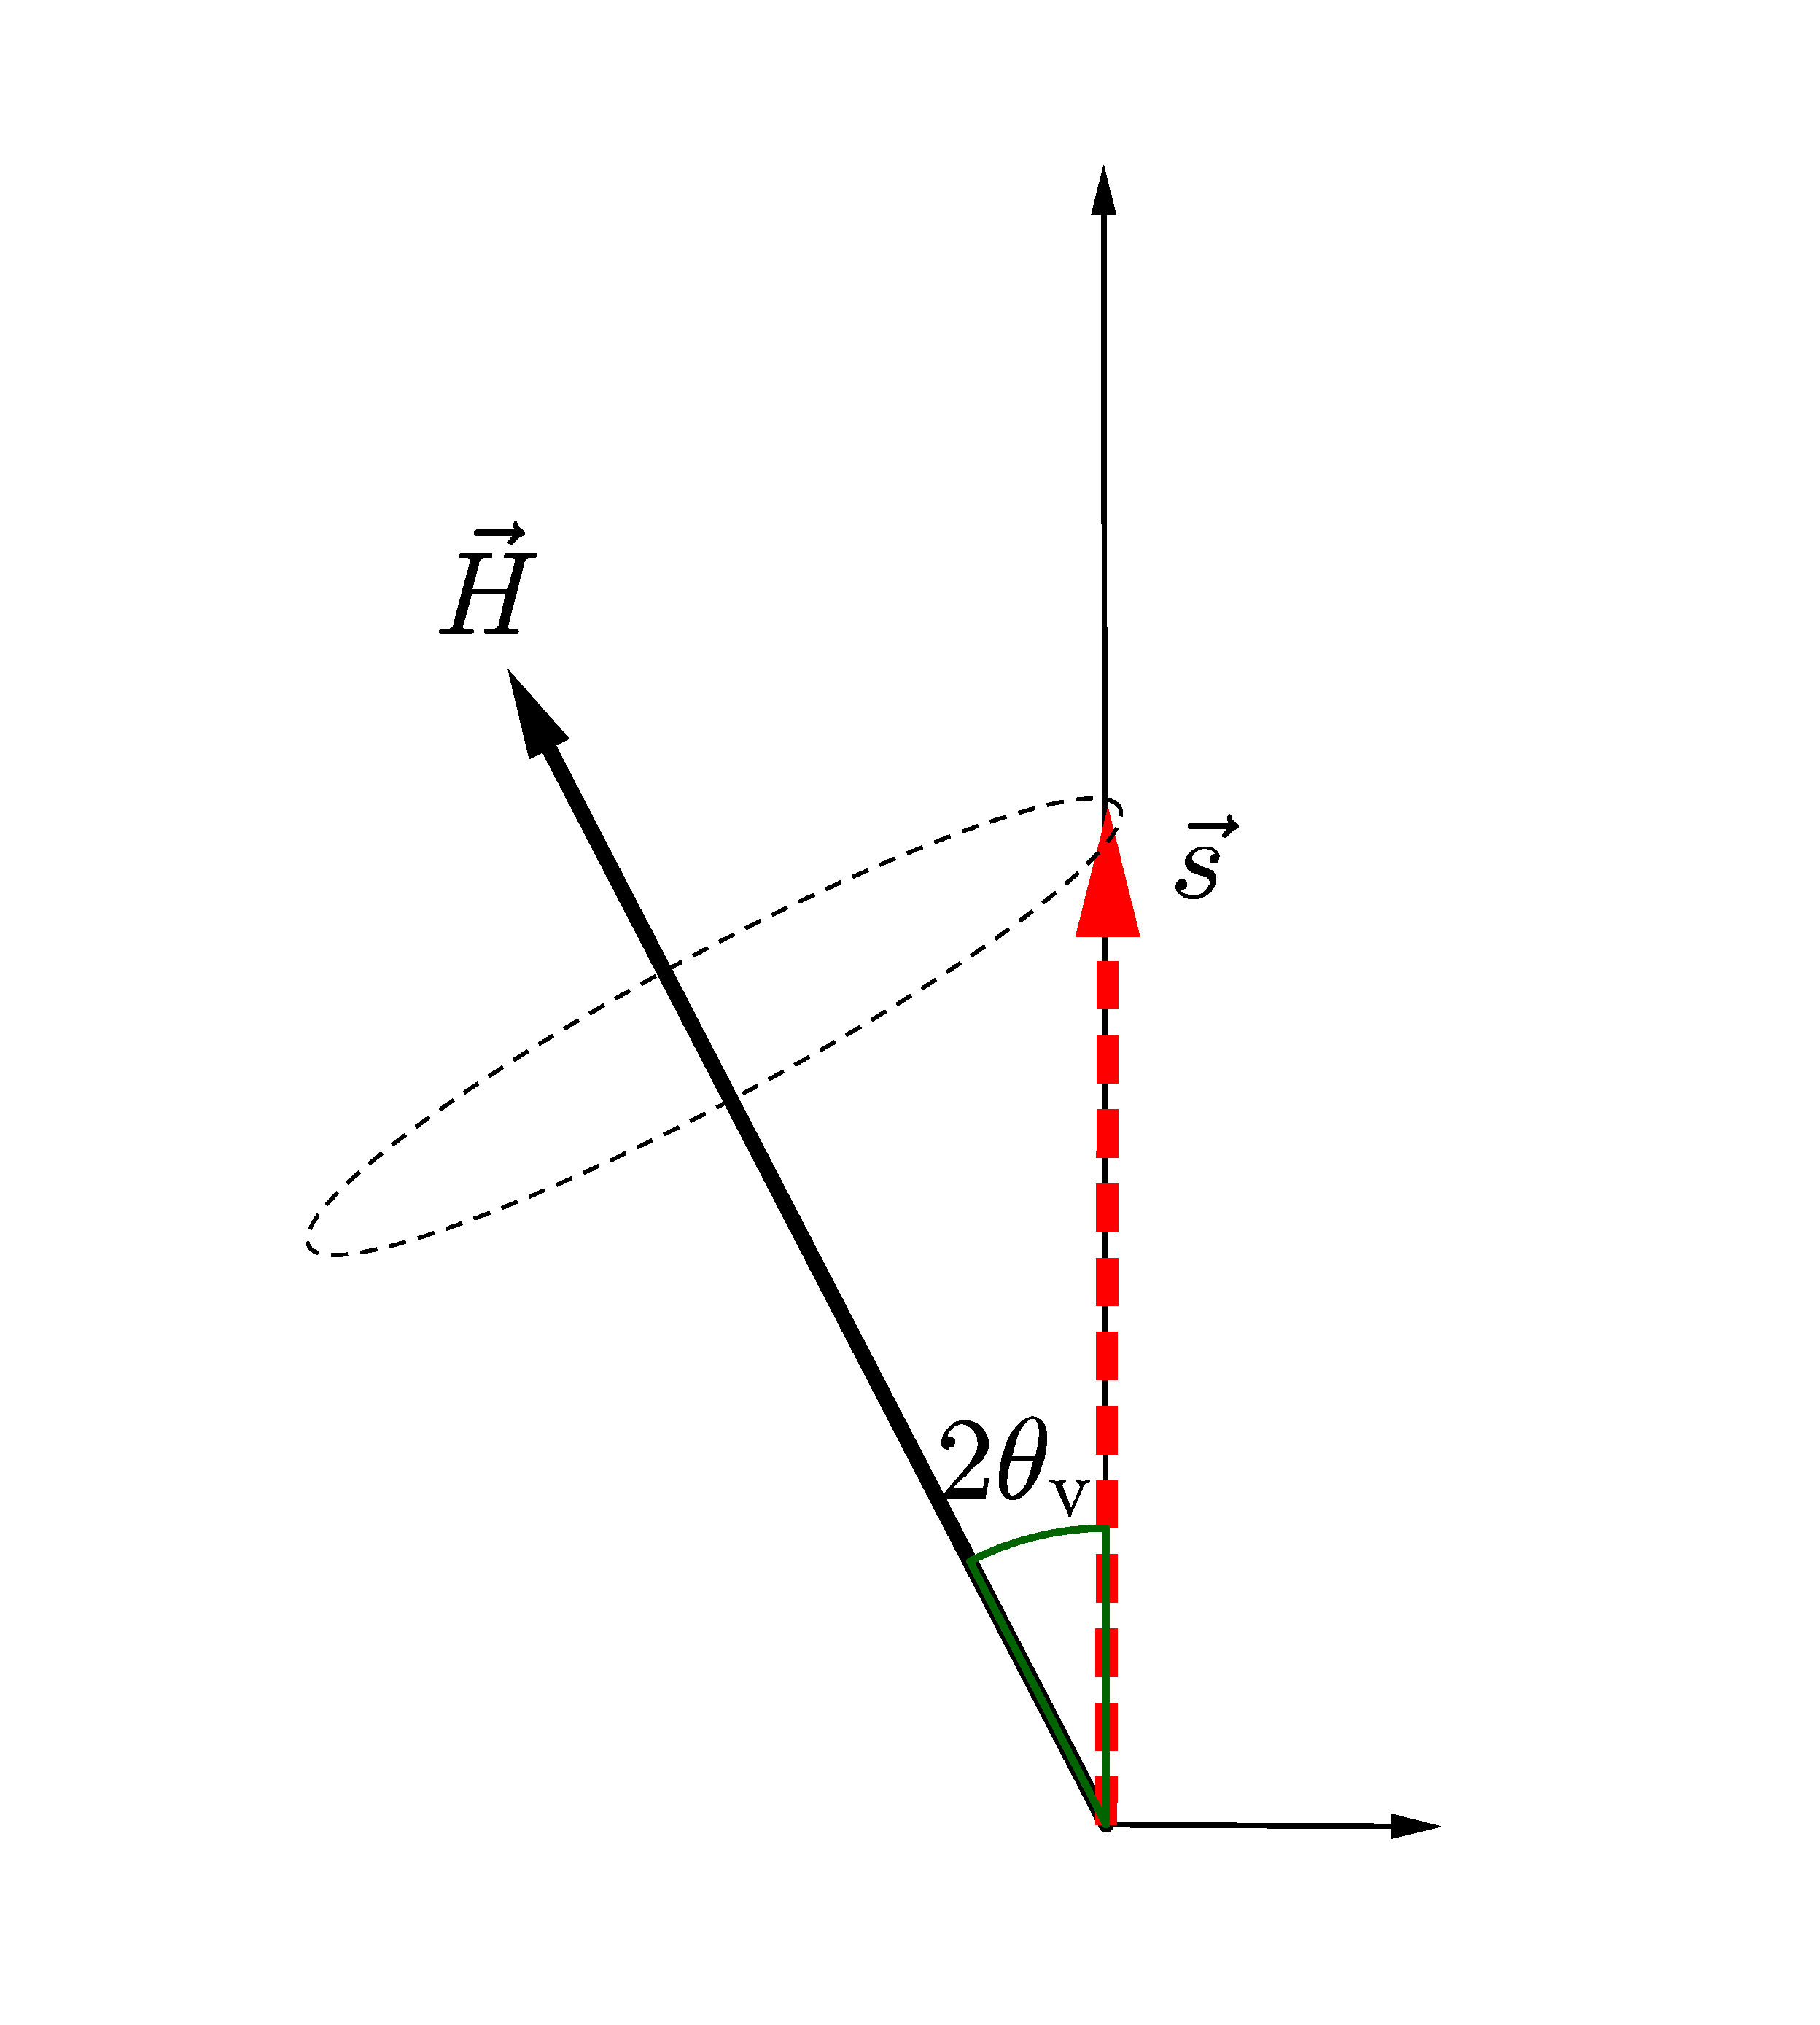
\includegraphics[width=0.6\textwidth]{chapters/assets/basics/flavor-isospin-vac-osc}
    \caption{Vacuum oscillations in the flavor isospin picture. The flavor isospin of a neutrino starting with the electron flavor precesses around the static ``Hamiltonian vecto
    r" $\vec H$, which gives a periodic flavor oscillation according to Eqn.~\eqref{chap:basics-eqn:vacuum-electron-probability}.}
    \label{chap:basics-sec:flavor-isospin-pic-fig:flavor-isospin-vac-osc}
\end{figure}
Therefore, the precession of the flavor isospin corresponds to a periodic oscillation between the two neutrino flavors (see Fig.~\ref{chap:basics-sec:flavor-isospin-pic-fig:flavor-isospin-vac-osc}).
%Eqn.~\eqref{chap:basics-sec:flavor-isospin-pic-eqn:eom-precession} depicts the precession of the flavor isospin for a neutrino which starts with the electron flavor and propagates in vacuum.
The oscillation frequency can be trivially read out from Eqn.~\eqref{chap:basics-sec:flavor-isospin-pic-eqn:eom-precession}:
\begin{equation}
\omega_\vv = \lvert \vec{H} \rvert.
\end{equation}




\begin{figure}[htbp]
    \centering
    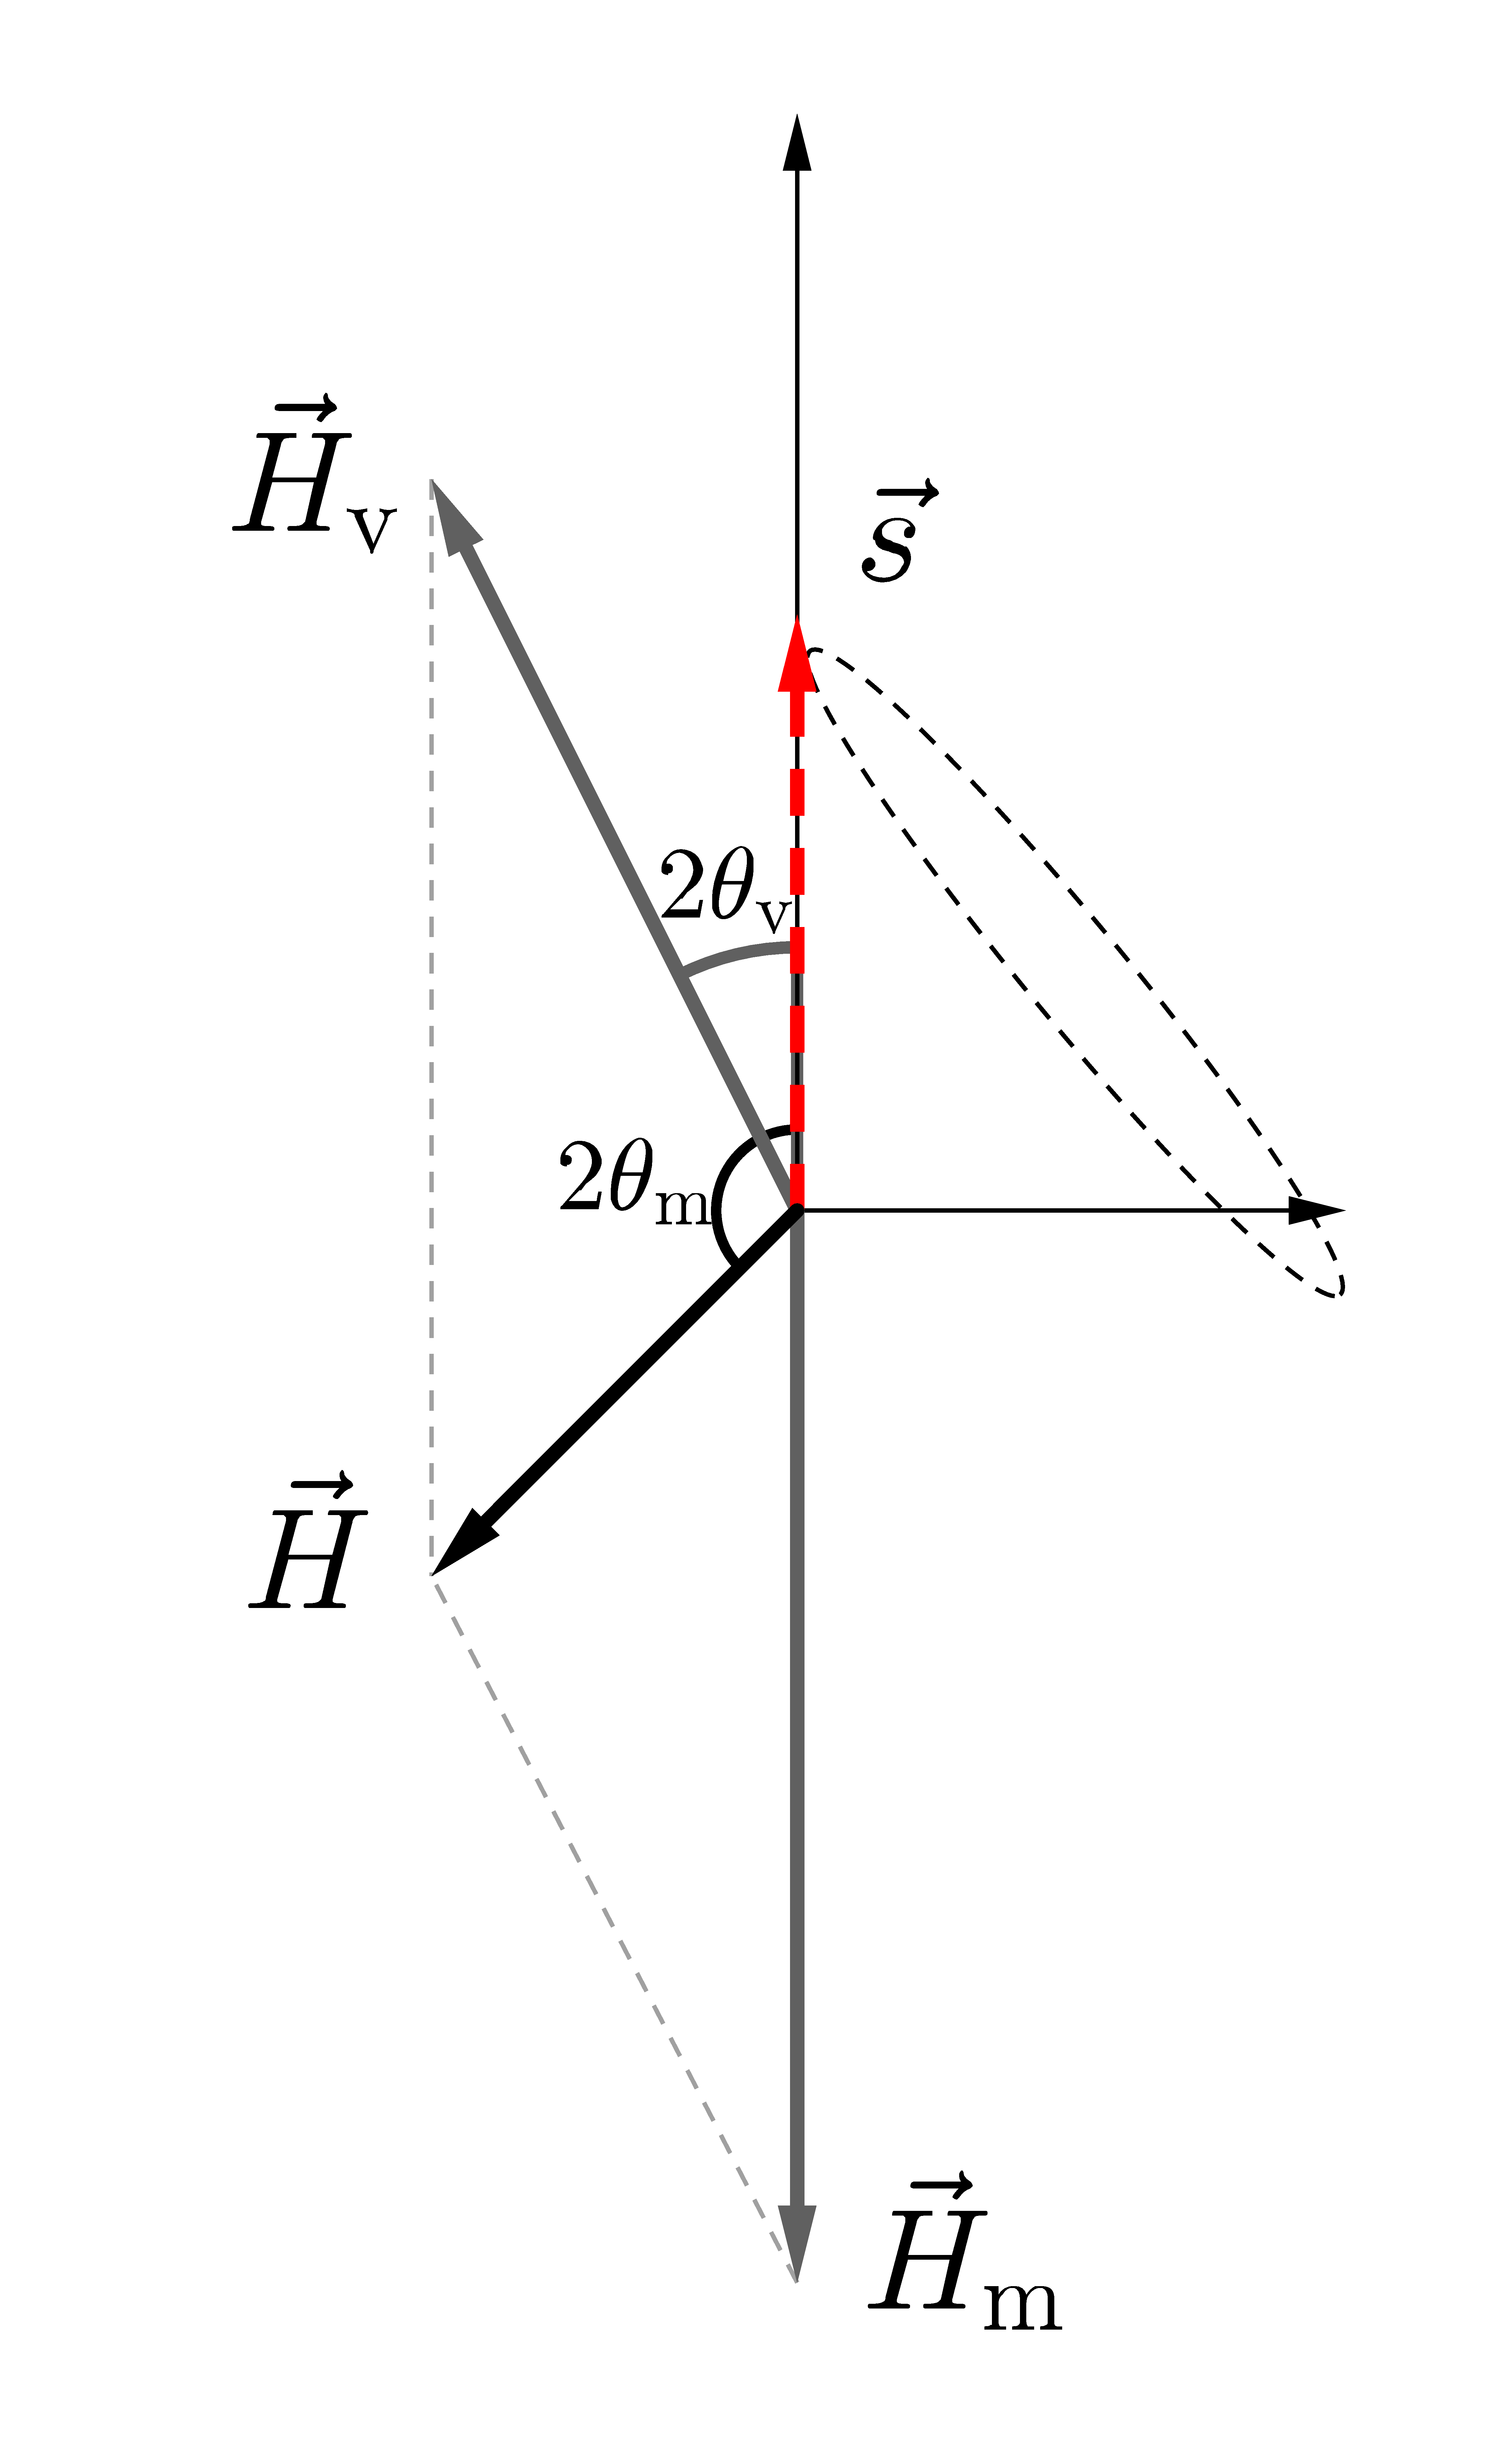
\includegraphics[width=0.4\textwidth]{chapters/assets/matter/matter-effect-notsolarge-density}
    \caption{Neutrino oscillations in flavor isospin picture with the presence of matter potential. The flavor isospin is denoted as red-dashed arrow. The two gray vectors stand for the vacuum Hamiltonians $\vec H_{\mathrm v}$ and matter potential $\vec H_{\mathrm m}$.}
    \label{chap:basics-sec:flavor-isospin-pic-fig:matter-effect-notsolarge-density}
\end{figure}

The MSW effect can also be easily explained using the flavor isospin picture. The Hamiltonian for the neutrino flavor evolution in the presence of dense matter is
\begin{align}
    &\mathsf H^{(\ff)} =  \frac{\omega_{\mathrm{v}}}{2}\left( - \cos 2\theta_{\mathrm{v}} {\sigma_3} + \sin 2\theta_{\mathrm{v}} {\sigma_1} \right)   + \frac{\lambda(x)}{2} {\sigma_3} \\
    \Rightarrow &\vec H =  \vec H_{\mathrm v} + \vec H_{\mathrm m}(x)
     = \omega_{\mathrm v}\begin{pmatrix}
    - \sin 2\theta_{\mathrm v} \\
    0 \\
    \cos 2\theta_{\mathrm v}
    \end{pmatrix}   + \begin{pmatrix}
    0\\
    0\\
    - \lambda(x)
    \end{pmatrix}  ,
\end{align}
where $\vec H_{\mathrm v}$ is the vacuum Hamiltonian, and $\vec H_{\mathrm m}(x)$ is the matter potential. The precession motion of the flavor isospin of the neutrino in the presence of dense matter is visualized in Fig.~\ref{chap:basics-sec:flavor-isospin-pic-fig:matter-effect-notsolarge-density}. The MSW resonance condition in Eqn.~\eqref{chap:basics-eqn:msw-resonance} corresponds to the scenario that the overall ``Hamiltonian vector" $\vec H$ is perpendicular to the third axis in flavor space. In this case, the flavor isospin rotates in the plane spanned by the second and third axes which gives maximum flavor oscillations (see~Fig.~\ref{chap:basics-sec:flavor-isospin-pic-fig:msw-adiabatic-critical}).

\begin{figure}[h!t]
    \centering
    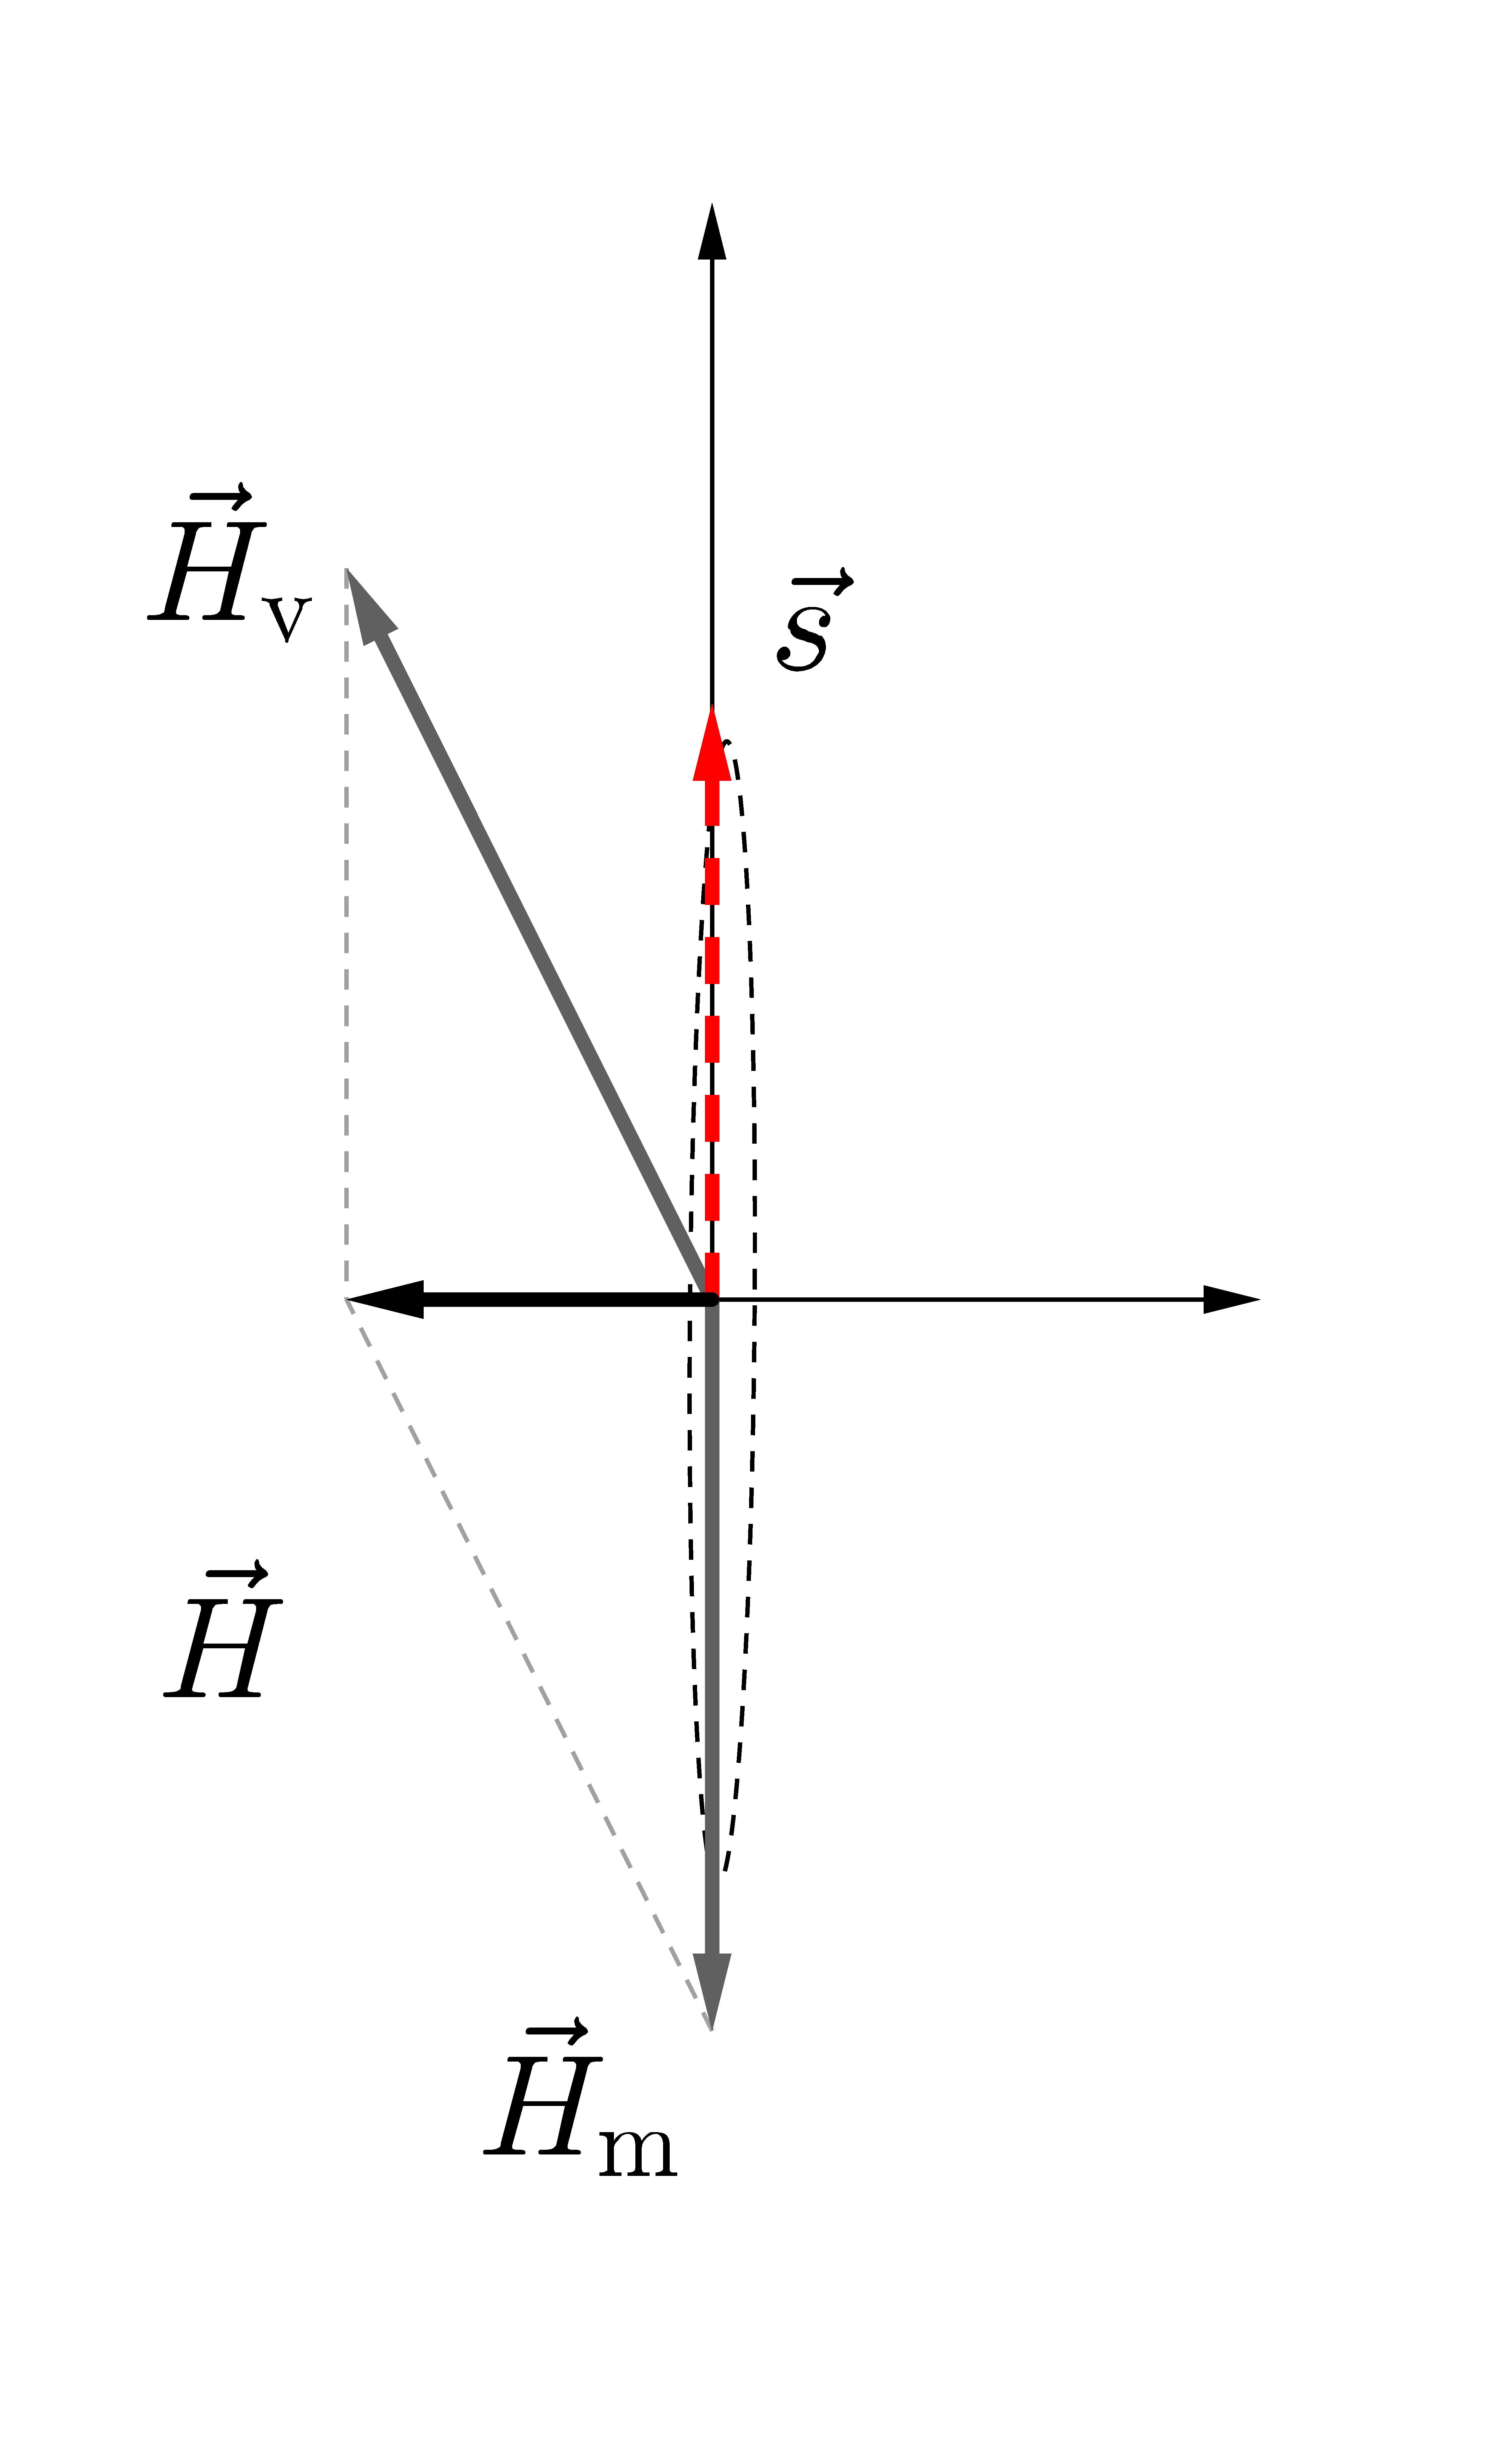
\includegraphics[width=0.4\textwidth]{chapters/assets/basics/matter-effect-critical-density}
    \caption{MSW resonance occurs when Eqn.~\eqref{chap:basics-eqn:msw-resonance} is satisfied.}
    \label{chap:basics-sec:flavor-isospin-pic-fig:msw-adiabatic-critical}
\end{figure}


The adiabatic flavor evolution of the neutrino in a varying matter density profile discussed in Sec.~\ref{chap:matter-sec:solar-neutrinos} can also be easily understood in the flavor-isospin picture.
In the region where the matter density is high, the total ``Hamiltonian vector" $\vec H$ points ``downward'' in flavor space. Therefore, a neutrino produced in the electron flavor will experience very little oscillations because its flavor isospin $\vec s$ is almost anti-parallel to $\vec H$ (see Fig.~\ref{chap:basics-sec:flavor-isospin-pic-fig:msw-adiabatic-large-density}). If the matter density along the propagation trajectory of the neutrino decreases slowly, $\vec s$ will stay almost anti-parallel to $\vec H$ as $\vec H$ rotates (see Fig.~\ref{chap:basics-sec:flavor-isospin-pic-fig:msw-adiabatic-medium-density}).
When the neutrino reaches the region with very low matter density, its flavor isospin becomes almost anti-parallel to $\vec H_{\vv}$, which implies that the neutrino is in $\ket{\nu_2}$ (see Fig.~\ref{chap:basics-sec:flavor-isospin-pic-fig:msw-adiabatic}).




\begin{figure}[htbp]
	\centering
	\begin{subfigure}[t]{0.3\textwidth}
		\centering
		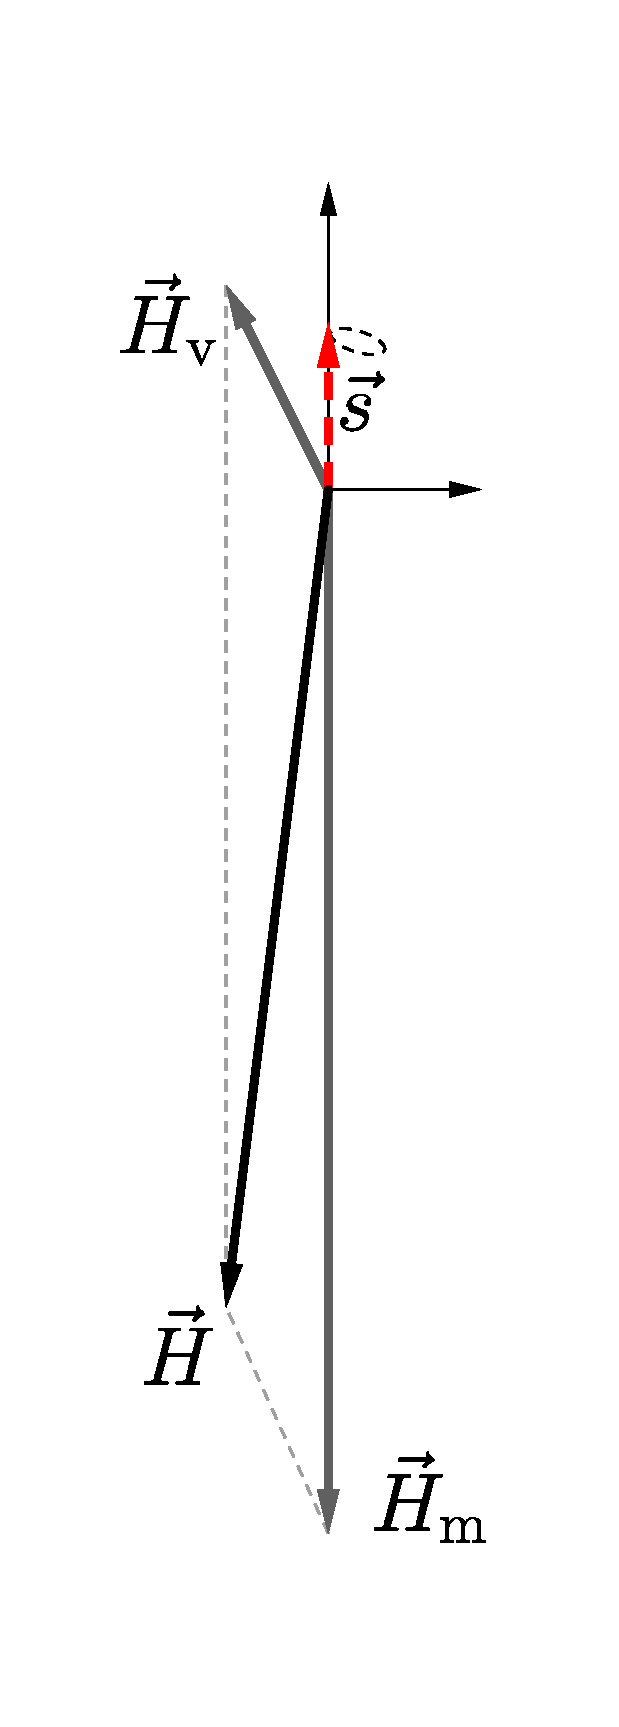
\includegraphics[width=0.8\textwidth]{chapters/assets/matter/matter-effect-large-density}
		\caption{High matter density}\label{chap:basics-sec:flavor-isospin-pic-fig:msw-adiabatic-large-density}
	\end{subfigure}%
	\begin{subfigure}[t]{0.3\textwidth}
		\centering
		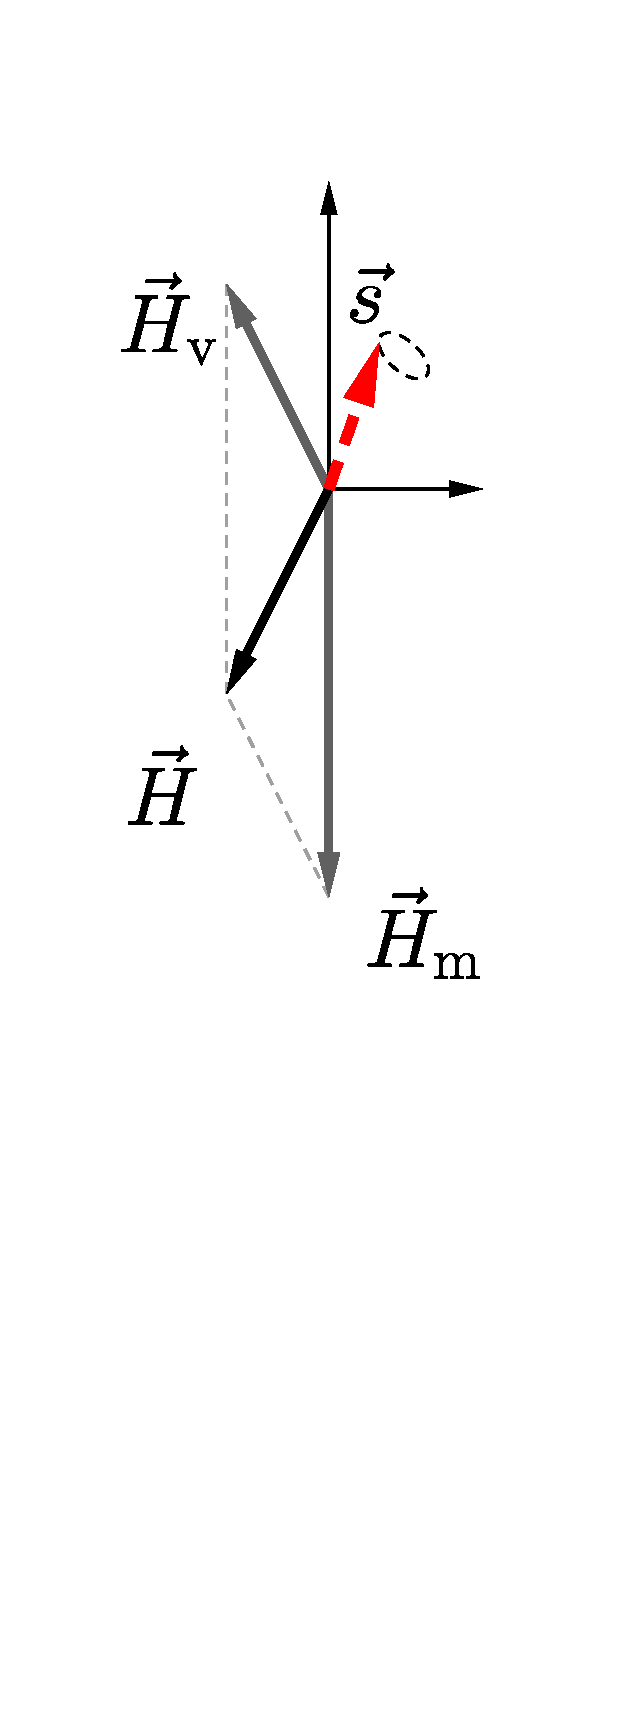
\includegraphics[width=0.8\textwidth]{chapters/assets/matter/matter-effect-adiabatic}
		\caption{Medium matter density}\label{chap:basics-sec:flavor-isospin-pic-fig:msw-adiabatic-medium-density}
	\end{subfigure}%
	\begin{subfigure}[t]{0.3\textwidth}
		\centering
    \vspace*{-3.93in}
		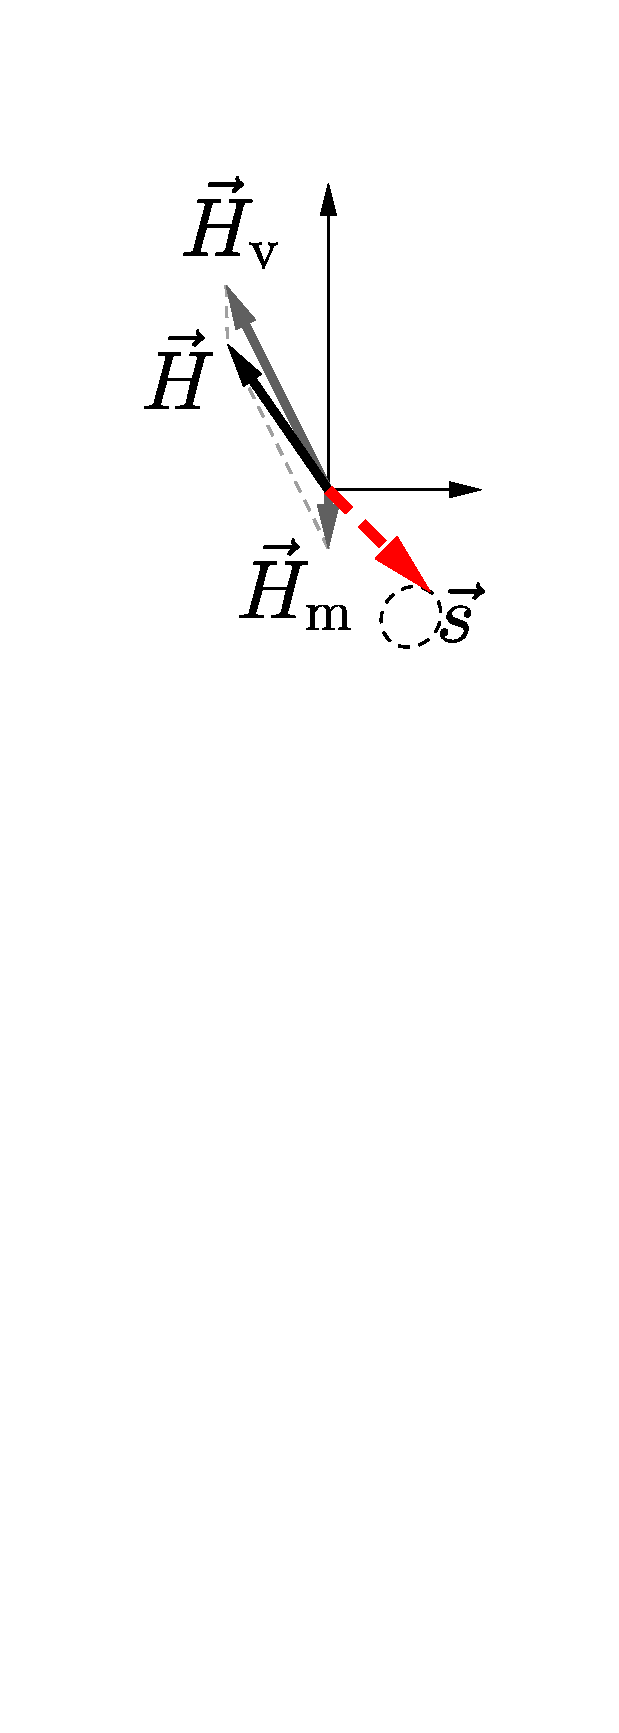
\includegraphics[width=0.8\textwidth]{chapters/assets/matter/matter-effect-adiabatic-3}
    \vspace*{-0.05in}
		\caption{Low matter density}\label{chap:basics-sec:flavor-isospin-pic-fig:msw-adiabatic-small-density}
	\end{subfigure}
	\caption{Flavor isospin picture of neutrino oscillations in matter. $\vec H_{\mathrm v}$ is the vacuum Hamiltonian, and $\vec H_{\mathrm m}$ is the matter potential.}\label{chap:basics-sec:flavor-isospin-pic-fig:msw-adiabatic}
\end{figure}






\section{Summary}

Neutrino oscillations in vacuum and in matter with a smooth profile have been explained. The neutrino oscillation phenomenon reveals a secret of the nature of the neutrino, i.e., its flavor states are not the same as the mass eigenstates of the Hamiltonian.
As a result, a neutrino produced in the pure flavor state through weak interaction will not remain in the same flavor state as it propagates, but oscillates between different flavors. The problem of neutrino oscillations in an environment with rapidly varying matter densities is significantly more difficult than that in a smooth profile. This will be discussed in the next chapter.

%!TEX root = ../dissertation.tex

\chapter{\label{chap:matter}Neutrino Oscillations in Oscillatory Matter Profile}


As one of the most intense neutrino sources, supernova neutrinos experience turbulent matter density as they propagate through the explosion~\cite{Muller2015, Couch2015}, where the flavor conversion is modified by interactions with matter. Meanwhile, with neutrinos depositing energy into the shock, neutrino flavor conversion is crucial to understand the shock evolution of supernova explosion. The turbulent matter density environment for neutrino flavor conversion has been studied~\cite{Loreti1994, Friedland2006,Kneller2010}. Recently, neutrino flavor conversions in matter background in varying matter density has been researched using a Jacobi-Anger expansion by Kneller, et al.~\cite{Kneller2013,Patton2014}. They have shown that neutrinos might go through large conversions between the two energy eigenstates.



I will take a step further and interpret parametric resonance~\cite{Akhmedov2000, Krastev1989} as well as other matter stimulated neutrino flavor conversions~\cite{Kneller2013, Patton2014}, as a superposition of Rabi oscillations. I will also calculate the criteria for the survival of resonance due to interference effect between different Rabi oscillation modes. In Sec.~\ref{chap:matter-sec:background}, we define the formalism of neutrino flavor conversions in matter used in this chapter where the equation of motion and Hamiltonian for neutrino flavor conversion in matter are explicitly written. In Sec.~\ref{chap:matter-sec:single} we discuss how neutrino flavor conversions are related to Rabi oscillations. To begin, we discuss a system with single frequency matter density fluctuation. We will show that such a system can be reduced to Rabi oscillations if resonance occurs. In Sec.~\ref{sec:multiple} we describe the interference effect between different frequencies of Rabi oscillations and develop the criteria for significant interference between two frequencies. We show that the interference between the many frequencies fits into the criteria we proposed for interference. In Sec.~\ref{sec:jacobi} we discuss the technique of decomposing the neutrino flavor conversions into summation of Rabi oscillations, by applying a specific unitary transformation and the Jacobi-Anger expansion. As the system is exactly decomposed into multiple Rabi oscillations, we can interpret neutrino flavor oscillations in any matter density fluctuations, in principle. As an example, we solve the neutrino flavor transitions in a castle wall matter profile, which contains infinite frequencies from the aspect of Fourier series.



% \section{\label{chap:basics-section:astro}Stars as Neutrino Factories}


% In the following sections of this chapter, I will discuss neutrino oscillations in the Sun as well as in supernovae. Solar neutrinos go through a region with smoothly decreasing matter density while supernova neutrinos go through a region with turbulent matter background~\cite{Friedland2006,Borriello2014}. Neutrino oscillations within the supernova is quite different from neutrino oscillations in the Sun.




\section{\label{chap:matter-sec:background}Equation of Motion for Neutrino Oscillations in the Matter}

% \fbox{TODO: Explain why two flavor} didn't add this because the three flavor is really very different.

I will write down the equation of motion for neutrinos prograting through a general matter profile $\lambda(r)$ where $r$ is the trajectory of neutrinos. The Hamiltonian of neutrino oscillations is Eqn.~\ref{chap:basics-sec:msw-eqn:hamiltonian-matter-effect}. The dynamics of neutrino flavor conversion is determined by the Schr\"{o}dinger equation:
\begin{equation*}
    \mathrm i\frac{\mathrm d}{\mathrm d r}\Psi(r) = \frac{1}{2} \left(
    (- \omega_{\mathrm{v}}\cos 2\theta_{\mathrm{v}} + \lambda(r) ) \sigma_3 + \omega_{\mathrm{v}}\sin 2\theta_{\mathrm{v}} \sigma_1
    \right)
    \Psi(r),
\end{equation*}
where $\Psi(r)$ is the wave function in flavor basis. For the two flavor scenario, the wave function is written as
\begin{equation}
	 \Psi(r) = \begin{pmatrix}
    \psi_{\ee} \\
    \psi_{\xx}
	\end{pmatrix},
\end{equation}
where $\psi_{\ee}$ and $\psi_{\xx}$ are the amplitudes for electron flavor and the other flavor ($\mu$ flavor or $\tau$ flavor) respectively.

For a general matter profile, it can always be expanded as the uniform zeroth mode and the higher modes. For the purpose of this section, I will denote the uniform zeroth mode as $\lambda_0$ and the $r$ dependent modes as $\delta \lambda(r)$, i.e.,
\begin{equation}
    \lambda(r) = \lambda_0 + \delta \lambda(r).
    \label{eq-general-matter-profile}
\end{equation}
I will constrate on the case where fluctuation $\delta \lambda(r)$ is a perturbation to the uniform matter potential.
To get a better understanding of the transition between the different neutrino states as a consequence of the fluctuation of matter density $\delta r(r)$, I define the background matter basis, in which the Hamiltonian is diagonalized in the absence of fluctuations $\delta\lambda(r)$, so that the Hamiltonian reads
\begin{equation}
    \mathsf H^{(\mathrm{m})} = -\frac{\omega_\mm}{2} \sigma_3 + \frac{1}{2} \delta\lambda(r) \cos 2\theta_{\mathrm m} \sigma_3
     - \frac{1}{2} \delta\lambda(r) \sin 2\theta_{\mathrm m} \sigma_1,
    \label{eq-hamiltonian-bg-matter-basis-general}
\end{equation}
where $\theta_{\mathrm m}$ is the mixing angle in a uniform matter profile $\lambda_0$, which is calculated using relation
\begin{equation*}
\tan 2\theta_{\mathrm{m}}=\sin 2\theta_{\mathrm v}/\left( \cos 2\theta_{\mathrm v} - \lambda_0/\omega_{\mathrm v} \right)
\end{equation*}
with $\omega_{\mathrm v}$ denoting the vacuum oscillation frequency and $\theta_{\mathrm v}$ denoting the vacuum mixing angle. The frequency $\omega_{\mathrm m}$ is defined as
\begin{equation}
\omega_{\mathrm{m}} = \omega_{\mathrm{v}} \sqrt{ ( \lambda_0/\omega_{\mathrm{v}} - \cos (2\theta_{\mathrm{v}}) )^2 + \sin^2(2\theta_{\mathrm{v}}) }.
\end{equation}

In the background matter basis, the wave function describes the amplitudes of different eigenstates defined when there is only background matter density $\lambda_0$. Given the transition probability between the these eigenstates, it is trivial to calculate the flavor conversion. Since I'll concentrate on the flavor conversion due to the matter fluctuations, I'll only discuss the transition between mass states in the background matter basis.

In this chapter, mixing angle is chosen so that $\sin^2(2\theta_{\mathrm v}) = 0.093$ and the mass squared difference is $\delta m^2 = 2.6\times 10^{-3}\mathrm{eV}^2$.




%%%%%%%%%%%%%%%%%%%%%%%%%%%%%%%%%%%%%%%%%%%%%%%%%%%%
%% Single frequency
%%%%%%%%%%%%%%%%%%%%%%%%%%%%%%%%%%%%%%%%%%%%%%%%%%%%



\section{\label{chap:matter-sec:single}Single Frequency Matter Profile and Rabi oscillations}%


In this section I will present a simple picture to explain neutrino parametric resonance in matter by utilizing the theory of Rabi oscillations which have been well studied in quantum optics~\cite{Boyd2008}. Rabi oscillations describe the transition between different energy levels due to an oscillatory external driving field, where maximum transition or resonance happens when the frequency of external driving field equals the energy gap. In Appendix~\ref{app:rabi-oscillations}, we derive the Rabi oscillation transition probabilities using neutrino flavor isospin method introduced in Ref.~\cite{Duan2006a}, and explained in Sec.~\ref{chap:basics-sec:flavor-isospin-pic}.




%%%%%%%%%%%%%%%%%%%%%%%%%%%%%%%%%%%%
%%%%%%%%% Rabi oscillation
%%%%%%%%%%%%%%%%%%%%%%%%%%%%%%%%%%%%


I will examine the neutrino flavor conversions in a single frequency matter profile $\delta\lambda(r) = \lambda_1 \cos(k_1 r)$. As will be proved in Sec.~\ref{sec:single-revisted}, the varying $\sigma_3$ term $\delta\lambda(r) \cos 2\theta_{\mathrm m} \sigma_3/2$ in Hamiltonian Eqn.~\ref{eq-hamiltonian-bg-matter-basis-general}, which is the varying energy gap due to varying matter density fluctuations, has little effect on the transition probabilities when the system is not far from resonance. With the varying $\sigma_3$ term removed, it indicates that this single frequency matter perturbation neutrino flavor conversion system has been reduced to a Rabi oscillation system, with external driving field frequencies $\pm k_1$ and energy gap $\omega_{\mathrm m}$. Mathematically, we can decompose $\cos( k_1 r )$ into two exponential functions so that we have two external driving frequencies $k_1$ and $-k_1$. By neglecting the off-resonance mode which has frequency $-k_1$, the Hamiltonian can be simplified,
\begin{align}
\mathsf H^{(\mathrm{m})} \to & -\frac{\omega_{\mathrm m}}{2} \sigma_3  - \frac{1}{2} \lambda_1 \sin 2\theta_{\mathrm m} \cos( k_1 r ) \sigma_1\label{eq-hamiltonian-bg-matter-basis-single-frequency} \\
\to & -\frac{\omega_{\mathrm m}}{2} \sigma_3  - \frac{1}{2} A_1 \exp (\mathrm ik_1 r) \sigma_1 \nonumber \\
= & -\frac{\omega_{\mathrm m}}{2} \sigma_3  - \frac{1}{2} A_1 \cos ( k_1 r)  \sigma_1 + \frac{1}{2} A_1\sin(k_1 r) \sigma_2,\nonumber
\end{align}
where
\begin{equation}
A_1 = \frac{\lambda_1 \sin 2\theta_{\mathrm m} }{2}.
\label{eq-define-a1}
\end{equation}

\begin{figure}[!htbp]
                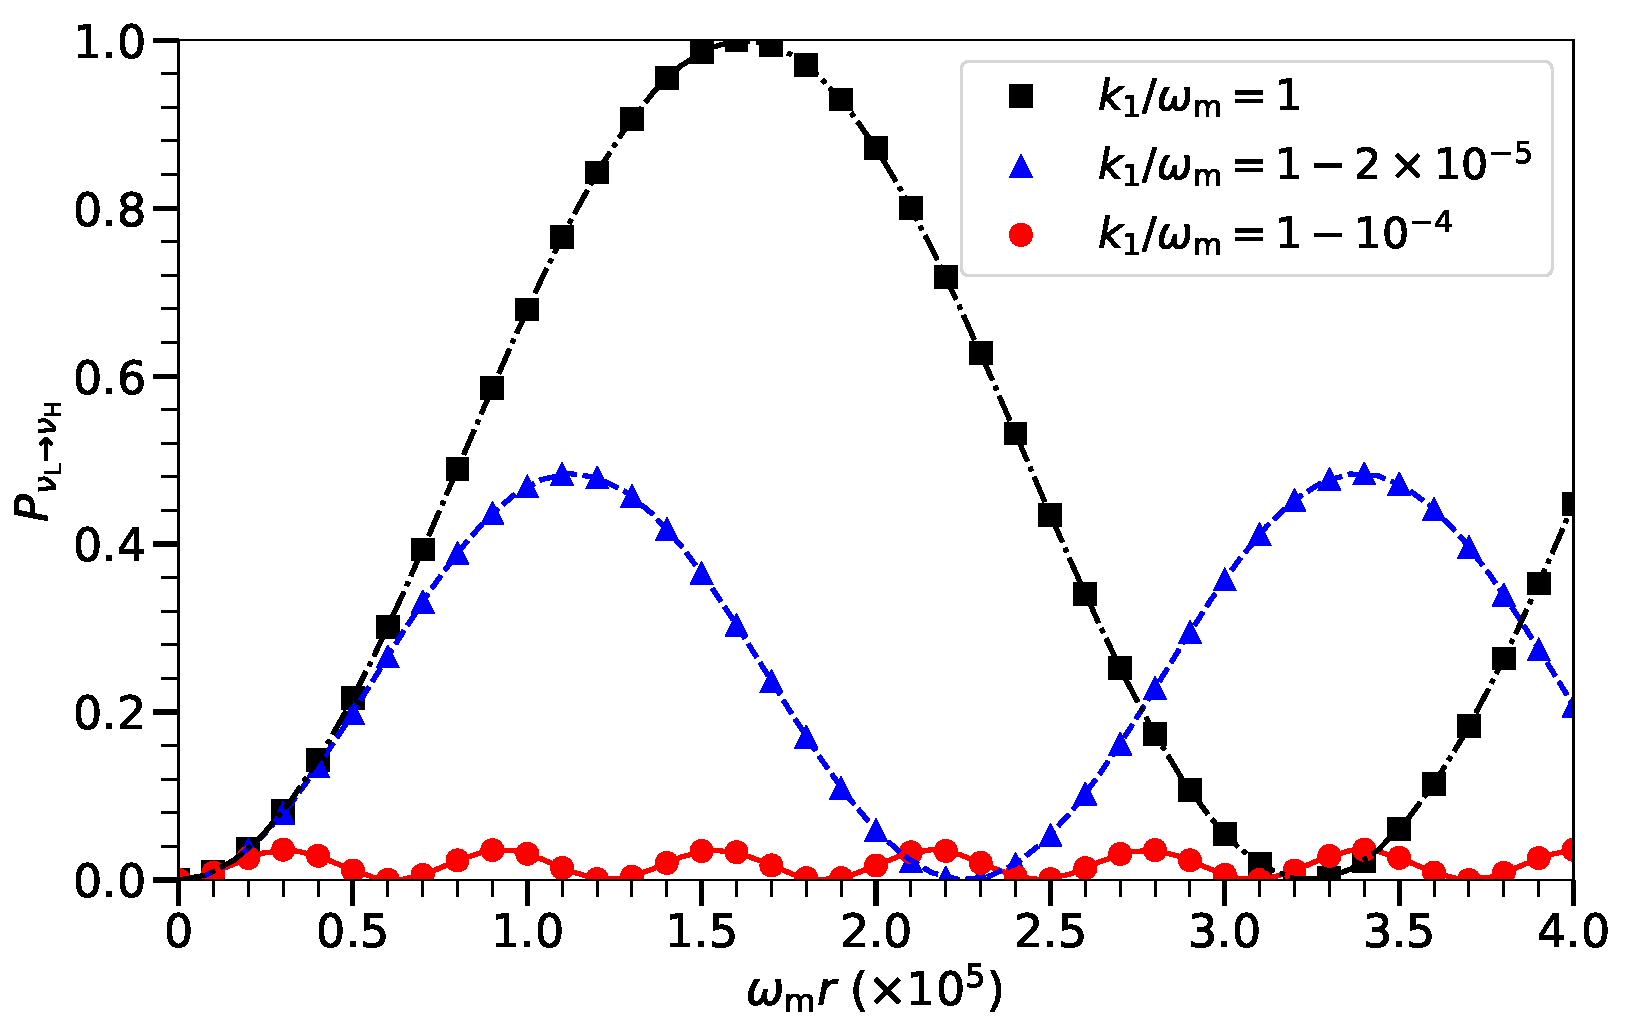
\includegraphics[width=\columnwidth]{chapters/assets/rabi/rabiOscillationsNeutrinoCoincidence-single-frequency}
                %rabiOscillationsNeutrinoCoincidence}
                \caption{Single frequency matter profile and Rabi oscillation. The markers are numerical results for the transition probabilities between two background mass eigenstates for the neutrinos with matter perturbation $A_1\sin(k_1 r)$. The dots, diamonds, and squares are for $k_1=\omega_{\mathrm m}$, $k_1=(1-2\times 10^{-5})\omega_{\mathrm m}$, and $k_1=(1-10^{-4})\omega_{\mathrm m}$ respectively. The lines are the predictions using Rabi formula. During the calculation, $\lambda_0$ is set to $0.5$ of the MSW resonance potential $\lambda_{\mathrm{MSW}}=\omega_{\mathrm{v}}\cos 2\theta_{\mathrm v}$ and mixing angle is chosen so that $\sin^2(2\theta_{\mathrm v}) = 0.093$.}
                \label{fig-rabiOscillationsNeutrinoCoincidence}
\end{figure}

The resonance condition is determined by matching the energy gap $\omega_{\mathrm m}$ with external driving field frequency $k_1$, i.e., $\omega_{\mathrm m} \sim k_1$. As the system approaches resonance condition, the transition probability between the two mass states should be predicted well using Rabi formula.

To show that this conjecture of simplifying neutrino flavor conversions to Rabi oscillations is correct, we calculate transition probabilities of the neutrinos described by Eqn.~\ref{eq-hamiltonian-bg-matter-basis-general} numerically, and compare them with Rabi formula Eqn.~\ref{rabi-system-transition-probability} from the Rabi oscillations described by Eqn.~\ref{rabi-oscillation-single-perturbation}.


In Fig.~\ref{fig-rabiOscillationsNeutrinoCoincidence}, I have plotted the numerical results using markers as well as the prediction using Rabi formula using lines. The agreement between numerical solutions of neutrino transitions between mass states and Rabi formula will be explained more precisely in Sec.~\ref{sec:jacobi}. For now, we address the significance of relative detuning $\RD = \lvert k_1 - \omega_{\mathrm m} \rvert /\lvert A_1 \rvert$,  which is rigoriously defined in Appendix~\ref{app:rabi-oscillations}. It measures how off-resonance a system is. $\RD\to 0$ indicates that the neutrino oscillation is very close to resonance, while $\RD\to \infty$ indicates that the neutrino oscillation is far away from resonance. The corresponding relative detunings are $0$, $1.0$, and $5.2$ for $k_1=\omega_{\mathrm{m}}$, $k_1=(1-2\times 10^{-5})\omega_{\mathrm m}$, and $k_1=(1-10^{-4})\omega_{\mathrm m}$.

% 0, 0.516197,1.03239,5.16197

For a single-frequency perturbation in the matter profile $\lambda(r) =\lambda_1 +  \lambda_1\sin(k_1 r)$, P. Krastev and A. Smirnov concluded that the parametric resonance condition is $\omega_{\mathrm{m}} \sim n k_1$, if instantaneous $\omega_{\mathrm{m,inst}}(r)$ associated with the matter profile at distance $r$ varies slowly~\cite{Krastev1989}. This condition is exactly the Rabi resonance condition when $n=1$, as such condition matches the driving field frequency to the energy split. Higher order effects are explained in Sec.~\ref{sec:single-revisted}.





\section{\label{sec:multiple}Interference Effects in Multi-frequency Matter Profiles}


The approach applied to single frequency matter profile also helps with the understanding of multi-frequency matter profile. However, multi-frequency matter profile leads to multiple modes of Rabi oscillations, even with our simplified approach by dropping the varying $\sigma_3$ term in Hamiltonian. In this section, we examine the interference between two modes of Rabi oscillations.
%Castle wall matter profile will serve as an example of multi-frequency profile to illustrate the idea of interference.



%%%%%%%%%
%%%% Interference
%%%%%%%%



%\subsection{\label{sec:interference-with-long-wavelength-mode}Interference Between Different Frequencies}

% \fbox{
% \parbox{0.9\columnwidth}{
% \begin{itemize}
%     \item Two limits: strong interference regime and low-interference regime
%     \item For strong interference we include multiple modes
%     \item For weak interference, we can interpret the case that one of the matter profile wavelength is much larger than the other. In this case we have a shift of background matter density of the short wavelength perturbation profile.
%     \item Examples. A slight shift in the background density could remove the resonance, which can be quantified.
%     \begin{equation*}
%         a
%     \end{equation*}
% \end{itemize}
% }
% }


I will explain the interference between different modes of Rabi oscillations using the idea of energy gap shift. Suppose I have a Rabi oscillation system with two modes, one of which is at resonance with frequency $k_1=\omega_{\mathrm m}$ and the other mode with frequency $k_2$ that is off resonance. In some cases, there can be a significant transition amplitude decrease because of the off resonance frequency $k_2$, which can be interpreted as shift of energy gap due to the frequency $k_2$. To model the effect, I construct a Rabi oscillation Hamiltonian with two modes of different frequency,
\begin{equation}
\mathsf H^{(\mathrm{m})}  = -\frac{\omega_{\mathrm{m}}}{2} \sigma_3 - \frac{1}{2} \sum_{n=1}^N  A_n \cos (k_n r) \sigma_1 + \frac{1}{2} \sum_{n=1}^N  A_n \sin (k_n r) \sigma_2,
\label{eq-hamiltonian-rabi-two-modes-interference}
\end{equation}
where $N=2$ for two frequency case. To show the destruction effect, the Hamiltonian Eqn.~\ref{eq-hamiltonian-rabi-two-modes-interference} is reformulated into a vector in flavor-isospin space,
\begin{equation}
\mathbf H = \mathbf H_3 + \mathbf H_1 +\mathbf H_2 = \begin{pmatrix}
0\\
0\\
\omega_\mm
\end{pmatrix} + \begin{pmatrix}
A_1 \cos (k_1 r)\\
-A_1 \sin (k_1 r)\\
0
\end{pmatrix} + \begin{pmatrix}
A_2 \cos (k_2 r)\\
-A_2 \sin (k_2 r)\\
0
\end{pmatrix}.
\end{equation}

The three terms are defined as $\mathbf H_3$, $\mathbf H_1$, and $\mathbf H_2$ respectively. $\mathbf H_1$ and $\mathbf H_2$ are two rotating vectors as a function of $r$ with frequencies $k_1$ and $k_2$ in this vector space, while $\mathbf H_3$ is perpendicular to $\mathbf H_1$ and $\mathbf H_2$. To work out the energy gap shift, we go to the frame that corotates with $\mathbf H_2$, in which we have the new frequencies $k_1'=k_1-k_2$ and $k_2'=0$ as well as new energy gap $\omega_{\mathrm m}' = \omega_{\mathrm m}- k_2$. The resonance mode $\mathbf H_1$ retains on the resonance condition since $k_1'=\omega_{\mathrm m}'$, i.e. $k_1-k_2 = \omega_{\mathrm m}-k_2$, holds in the new frame. On the other hand, we have two static fields $\mathbf H_3$ and $\mathbf H_2$ together as the new energy gap, as long as $\mathbf H_2\ll \mathbf H_3$, which is the usual case. The new energy gap in this frame is calculated as
\begin{align}
    \tilde\omega_{\mathrm{m}}' =& \sign (\omega_{\mathrm m}') \sqrt{\omega_{\mathrm{m}}'^2 + A_2^2 } \nonumber\\
    \approx & \omega_{\mathrm{m}}' + \frac{A_2^2}{2\omega_{\mathrm m}'} \nonumber\\
    =& \omega_{\mathrm m} - k_2 + \frac{1}{2}\frac{A_2^2}{\omega_{\mathrm m} - k_2},
    \label{eq-new-energy-gap-due-to-second-mode-approximation}
\end{align}
where we kept only first order of Taylor series. The Taylor expansion in Eqn.~\ref{eq-new-energy-gap-due-to-second-mode-approximation} holds as long as the relative detuning for the second frequency is large which means the second frequency is off resonance. As an approximation, the transitions between the two energy states follows the Rabi oscillations with energy gap $\tilde \omega_{\mathrm m}'$ and driving field with frequency $k_1'=k_1-k_2$. Consequently, we can estimate how much the amplitude of the transition is suppressed due to $k_1$ mode by calculating the new relative detuning,
\begin{align}
    \RD' =& \frac{\lvert k_1' - \tilde \omega_{\mathrm m}' \rvert}{\lvert A_1 \rvert}\nonumber\\
    =& \left \lvert \frac{ k_1-\omega_{\mathrm m}}{ A_1} + \frac{ A_2^2 }{2  A_1 ( k_2 - \omega_{\mathrm m})} \right  \rvert\\
    =& \left \lvert  \frac{\sign({ k_1-\omega_{\mathrm m}})}{\sign (k_2 - \omega_{\mathrm m})} \RD_1 +  \frac{ A_2 }{2 A_1 \RD_2 }\right \rvert ,
    \label{eq-relative-detuning-changed}
\end{align}
where $\RD_2$ is the relative detuning of the second mode,
\begin{equation*}
\RD_i =  \left\lvert \frac{ k_i - \omega_{\mathrm m}}{A_i} \right \rvert.
\end{equation*}
In principle, the energy gap of the first frequency can be changed to approach the resonance or escape the resonance by carefully arranging the second frequency, which is also obvious from Eqn.~(\ref{eq-relative-detuning-changed}). For the purpose of the section we first discuss the most important destruction effect by choosing $\RD_1 = 0$. We observe the importance of the relative detuning. For the second mode to significantly interfere with the first mode, we need a small $\RD_2$ and a large amplitude or width $A_2\gg A_1$.

The condition can be verified by comparing the numerical solution and estimation using Rabi formula. However, we are most interested in the amplitude change due to $\mathbf H_2$ mode. Relative detuning is the only variable that we need to calculate the amplitude, hence we only compare the numerical results with estimated amplitudes using $1/(1+\RD'^2)$.
To verify the condition, we choose the first rotating perturbation to satisfy the resonance condition $k_1=\omega_{\mathrm{m}}$, the condition for the second rotating field shifting the system out of resonance is that the relative detuning becomes larger than $1$, which leads to
\begin{equation}
\lvert A_2 \rvert \geq \sqrt{2\omega_{\mathrm{m}} \lvert A_1 (k_2-\omega_{\mathrm m})\rvert} \equiv A_{2,\mathrm{Critical}}.
\end{equation}
We expect the transition amplitude to decrease as we have larger $\lvert A_2\rvert$.


\begin{figure}[!htbp]
                \centering
                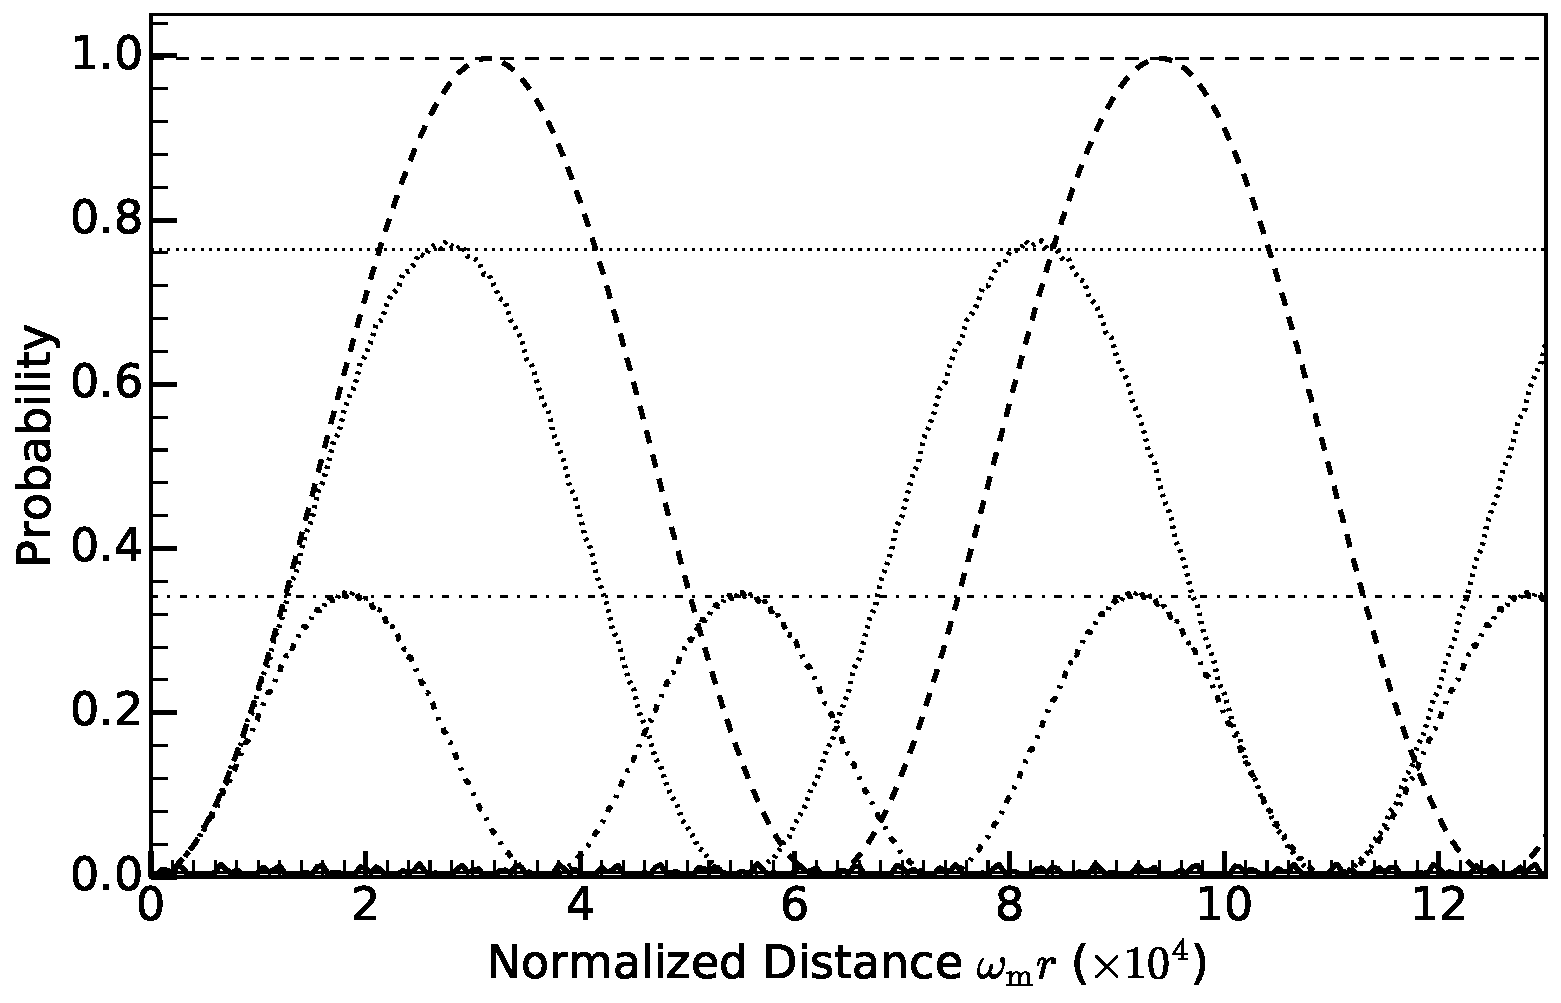
\includegraphics[width=\columnwidth]{chapters/assets/rabi/interference-reduction}
                \caption{Reduction of transition amplitudes due to interference. Dashed line, dotted line, dash-dotted line, and solid line are for $A_2=10^{-2}\omega_{\mathrm{m}}$, $k_2=10\omega_{\mathrm m}$, $A_2=10^{-2}\omega_{\mathrm{m}}$, $k_2=10^{-1}\omega_{\mathrm m}$, $A_2=5.0\times 10^{-2}\omega_{\mathrm{m}}$, $k_2=10\omega_{\mathrm m}$, and $A_2=5\times 10^{-2}\omega_{\mathrm{m}}$, $k_2=10^{-1}\omega_{\mathrm m}$. In all the calculations, we choose $A_1=10^{-4}\omega_{\mathrm m}$, $k_1=\omega_{\mathrm m}$. The grid lines are the transition amplitudes estimated using $\RD'$. During the calculation, $\Lambda_0$ is set to half of the MSW resonance potential, $\Lambda_0 = \frac{1}{2}\lambda_{\mathrm{MSW}}=\frac{1}{2}\omega_{\mathrm{v}}\cos 2\theta_{\mathrm v}$.}
                \label{fig-rabi-oscillations-energy-gap-change}
\end{figure}


We choose the two modes where the first one has amplitude $A_1 = 10^{-4}\omega_{\mathrm{m}}$ and frequency $k_1 = \omega_{\mathrm{m}}$. With a small amplitude of the second frequency, $A_2=10^{-4}\omega_{\mathrm{m}}$, and large frequency $k_2=10\omega_{\mathrm{m}}$, we obtain almost full resonance. For larger $A_2$ the destruction effect is more effective, as shown in Fig.~\ref{fig-rabi-oscillations-energy-gap-change}. The estimations of transition amplitude are in good agreement with the numerical results. To show the importance of relative detuning, we calculated the relative detuning for each cases, which are $0.06$, $0.6$, $1.4$, $13.9$ for the lines from top to down. We also notice that the width of each cases doesn't change since we kept $A_1$ fixed for each calculation, which indicates that the decreasing in transition amplitude is because of the increasing in detuning.

Even for the single frequency matter profile, there are two modes of Rabi oscillations $\pm k_1$, under the approximation that the varying $\sigma_3$ term in Hamiltonian is neglected, as mentioned in Sec.~\ref{chap:matter-sec:single}. The three examples calculated in Fig.~\ref{fig-rabiOscillationsNeutrinoCoincidence} are almost exact since the modification of relative detuning for the $k_1$ mode that we kept, due to the far off resonance mode $-k_1$ that we neglected, is tiny. The first two lines of Table.~\ref{tab-q-values-single-frequency-example} show the relative detunings of the three cases in Fig.~\ref{fig-rabiOscillationsNeutrinoCoincidence}, where $n=\pm 1$ are for the $\pm k_1$ modes in the Hamiltonian Eqn.~\ref{eq-hamiltonian-bg-matter-basis-single-frequency}. We observe in Fig.~\ref{fig-rabiOscillationsNeutrinoCoincidence} that the relative detuning change due to an extra $-k_1$ mode is not observable.


% \section{\label{chap:matter-sec:constructive}Constructive Effects}
\begin{figure}[!htbp]
    \centering
    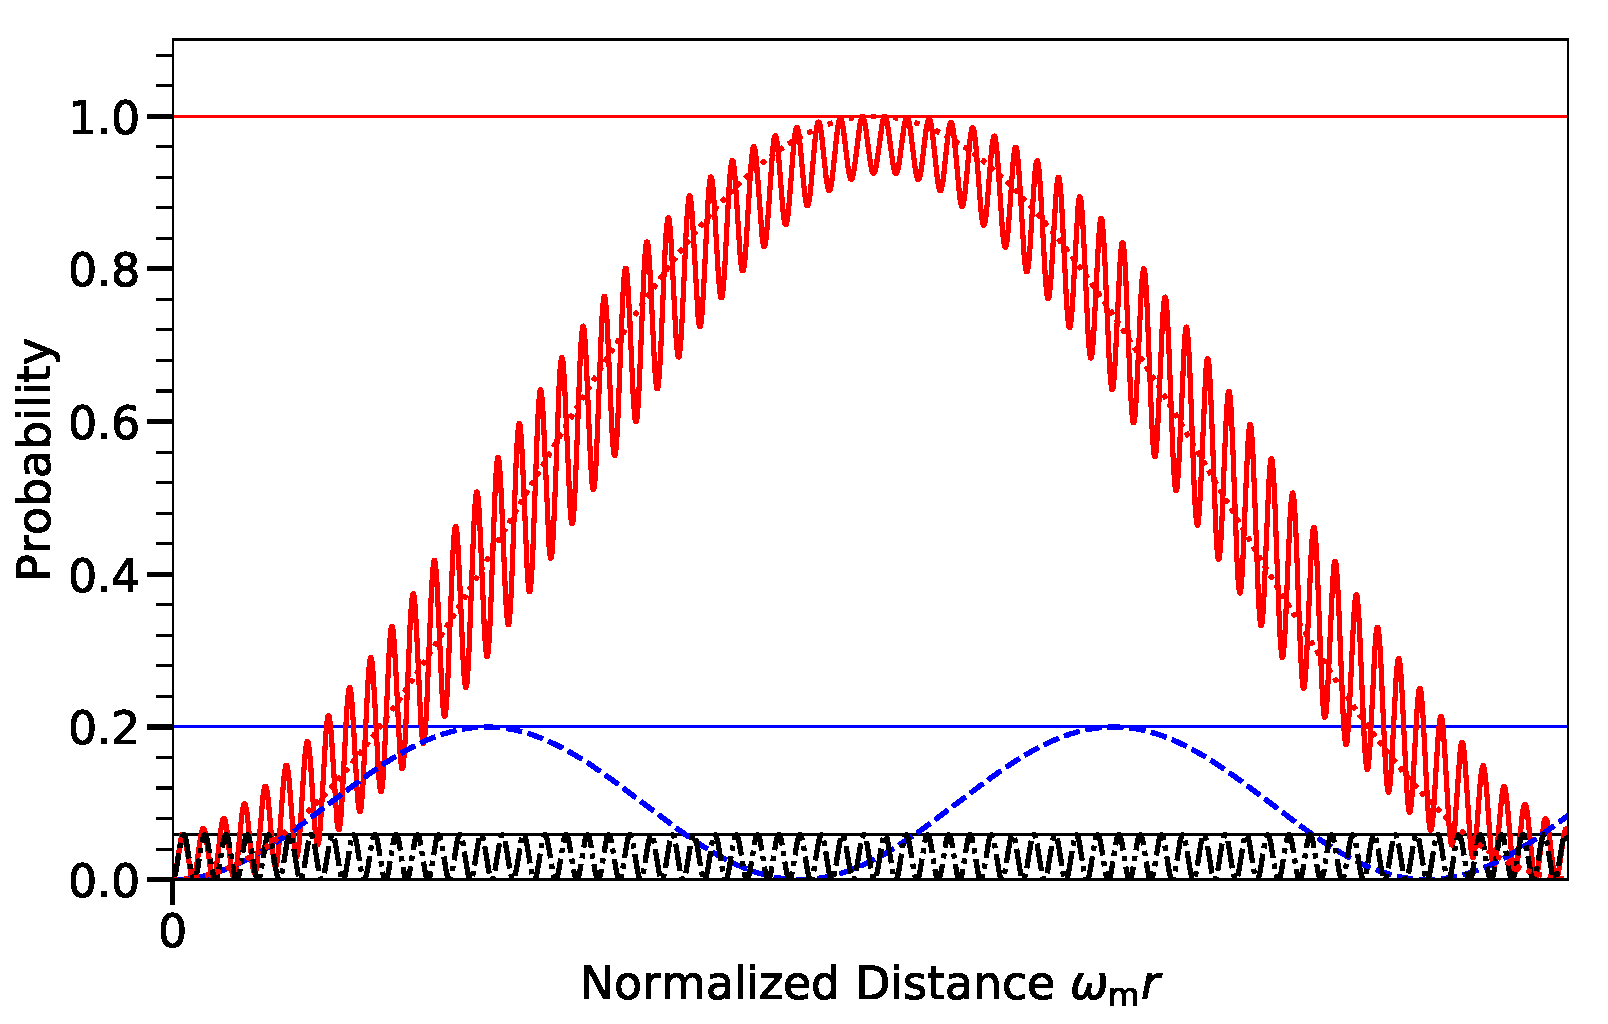
\includegraphics[width=\textwidth]{chapters/assets/rabi/rabiOscillationsNeutrinoCoincidence-two-frequencies-constructive.pdf}
    \caption{Constructive interference for two frequencies in matter density profile. The solid red line, dashed blue line, dash-dotted black line, are the transition probability for two frequencies combined, the first frequency $k_1$ only, the second frequency $k_2$ only. The amplitudes of each frequency are $A_1=0.4$, $A_2=2.6$ respectively. The grid lines are the oscillations amplitudes predicted by Rabi formula. The dotted red line is the oscillations predicted by Rabi formula for the two combined frequencies.}
    \label{chap:matter-sec:constructive-fig:two-frequencies-constructive}
\end{figure}

Adding a second frequency to the matter density profile can also be constructive. I calculated an example with two frequencies in matter density profile, so that the Hamiltonian is
\begin{equation*}
    \mathsf H^{(\mm)} = - \frac{\omega_{\mathrm m}}{2} \sigma_3 - \left(\frac{A_1}{2}\cos(k_1 r) + \frac{A_2}{2}\cos(k_2 r) \right) \sigma_1 + \left( \frac{A_1}{2}\sin(k_1 r) + \frac{A_2}{2}\sin(k_2 r) \right) \sigma_2.
\end{equation*}
We choose two matter profile frequencies that are off resonance and producing large relative detuning,
% k1_0.95_k2_2.6_a1_0.025_a2_0.4
\begin{equation}
    A_1 = 0.025, \qquad k_1 = 0.95, \qquad A_1 = 0.4, \qquad k_2 = 2.6.
\end{equation}
The oscillation amplitude for each mode being much smaller than 1. However, the combined two frequencies case produces oscillations are resonance (c.f.~Fig.~\ref{chap:matter-sec:constructive-fig:two-frequencies-constructive}), since the relative detuning for the combined two frequencies case is 0.



%%%%%%%%%%%%%%%%%%%%%%%%%%%%%%%%%%%%%%%%%%%%%%%%%%%%
%%%%%%%%%  Stimulated Neutrino Oscillations  %%%%%%%%%%%%%%%%%%%
%%%%%%%%%%%%%%%%%%%%%%%%%%%%%%%%%%%%%%%%%%%%%%%%%%%%

\section{\label{sec:jacobi}Parametric Resonance and Rabi oscillation --- Jacobi-Anger expansion}


With the intuition of the Rabi oscillations itself as well as the interference between different modes of Rabi oscillations shown in Sec.~\ref{sec:multiple}, I can interpret the transition probabilities of any matter profile more precisely if the system can be exactly decomposed into multiple Rabi oscillations. Kneller et. al provided a method to achieve this goal~\cite{Kneller2013}, namely the Jacobi-Anger expansion. In this section, I will show that the matter effect can be decomposed into superpositions of Rabi oscillations by applying a Jacobi-Anger expansion to the Hamiltonian. Our approach is to apply a designed unitary transformation first which make the motivation of Jacobi-Anger expansion, before writing down the final result as superpositions of Rabi oscillation using Jacobi-Anger expansion. For a system with general matter perturbation (see Eqn.~\ref{eq-hamiltonian-bg-matter-basis-general}), we apply an unitary transformation of the form
\begin{equation}
    \mathbf{U} =  \begin{pmatrix} e^{-\ri \eta (r)} & 0 \\  0 & e^{\mathrm i \eta (r)}  \end{pmatrix},
    \label{eq-rabi-transformation}
\end{equation}
which is a transformation used in Ref.~\cite{Kneller2006} to remove the diagonal elements of the Hamiltonian. This transformation is essentially a rotation $\exp\left(-\mathrm i\frac{\sigma_3}{2}\cdot 2\eta\right)$, thus it doesn't change $
\sigma_3$ terms themselves. In this work, this transformation is used to remove the varying $\sigma_3$ terms $\delta\lambda(r) \cos 2\theta_{\mathrm m} \sigma_3/2$ in the Hamiltonian, so that the energy gap is fixed in the new basis $\left(\ket{\nu_{\mathrm{r1}}},\ket{\nu_{\mathrm{r2}}}\right)^{\mathrm{T}}$, which is defined as
\begin{equation}
    \begin{pmatrix} \ket{\nu_{\mathrm{r1}}}\\ \ket{\nu_{\mathrm{r2}}} \end{pmatrix} =  \mathbf{U}^\dagger \begin{pmatrix} \ket{\nu_{\mathrm{L}}} \\ \ket{\nu_{\mathrm{H}}} \end{pmatrix}.
    \label{eq-rabi-basis}
\end{equation}
For convenience, we name this unitary transformation in Eqn.~(\ref{eq-rabi-transformation}) Rabi transformation as well as the new basis in Eqn.~(\ref{eq-rabi-basis}) the Rabi basis. The reason it can remove the $\sigma_3$ term is that it will transform the system into a rotating frame so that the varying energy gap due to the fluctuating matter density is exactly cancelled by rotation of the frame. Another advantage of this transformation is that the transition probability from light state to heavy state in background matter basis is easily calculated as $P_{\mathrm{L} \to
\mathrm{H}} (x) = \lvert e^{i\eta} \psi_{\mathrm r2} (x)  \rvert^2 = \lvert \psi_{\mathrm r2} (x)  \rvert^2 .$. In Rabi basis, we find the Schr\"{o}dinger equation
\begin{align*}
    &\begin{pmatrix}  \frac{\mathrm d\eta}{\mathrm dr}  & 0 \\ 0 & - \frac{\mathrm d\eta}{\mathrm d r}  \end{pmatrix} \begin{pmatrix} \psi_{\mathrm R1} \\ \psi_{\mathrm R2} \end{pmatrix} + \mathrm i \frac{\mathrm d}{\mathrm dr} \begin{pmatrix} \psi_{\mathrm R1} \\ \psi_{\mathrm R2} \end{pmatrix} \\
    =& \left[ -\frac{\omega_{\mathrm m} }{2} \sigma_3  + \frac{\delta \lambda}{2} \cos 2\theta_{\mathrm m}  \sigma_3  - \frac{\delta \lambda}{2} \sin 2\theta_{\mathrm m} \begin{pmatrix} 0 & e^{2\mathrm i\eta} \\ e^{-2 \mathrm i\eta } & 0 \end{pmatrix}   \right] \begin{pmatrix} \psi_{\mathrm R1} \\ \psi_{\mathrm R2} \end{pmatrix},
\end{align*}
in which the varying diagonal elements in Hamiltonian can be eliminated by choosing $\eta(r)$ properly, i.e.,
\begin{equation}
    \eta(r) - \eta(0) =  \frac{\cos 2\theta_{\mathrm{m}}}{2} \int_0^r \delta\lambda (\tau) d\tau.
\end{equation}
In Rabi basis, the Schr\"{o}dinger equation becomes
\begin{equation*}
    \ri \frac{d}{dr} \begin{pmatrix} \psi_{\mathrm r1} \\ \psi_{\mathrm r2} \end{pmatrix} = \left[ - \frac{\omega_{\mathrm m}}{2} \sigma_3 - \frac{\delta \lambda}{2} \sin 2\theta_{\mathrm m} \begin{pmatrix} 0 & e^{2\ri\eta} \\ e^{-2 \ri \eta } & 0 \end{pmatrix}\right] \begin{pmatrix} \psi_{\mathrm r1} \\ \psi_{\mathrm r2} \end{pmatrix}.
\end{equation*}
One can easily show that the transition probability between two eigenstates in Rabi basis is the same as the transition probability between two eigenstates in background matter basis, given the initial condition that the system is in low energy state.

For single frequency matter profile with potential $\delta\lambda(r) = A_1\sin(k_1 r)$, we have $\eta(r) = - A_1 \cos 2\theta_{\mathrm m} \cos (k_1 r)/(2 k) $. To make connection with Rabi oscillation, we apply Jacobi-Anger expansion, which is used in Ref.~\cite{Kneller2013}, to decompose the $\exp\left( \ri z \cos\left(k_1 r \right) \right)$-like term in Hamiltonian into linear combinations of terms that is proportional to $\exp\left(\ri n k_1 r \right)$, i.e., to decompose spherical waves into plane waves. The decomposed form of Hamiltonian explicitly shows that the Hamiltonian is a summation of Rabi systems, which is
\begin{equation}
    H^{(\mathrm{R})} =
    -\frac{\omega_{\mathrm{m}}}{2} \sigma_3
    -  \frac{1}{2} \sum_{n=-\infty}^\infty B_n \begin{pmatrix}
    0 &  \Phi_n e^{\ri n k_1  r} \\
     \Phi_n^* e^{ - \ri n k_1 r} & 0
    \end{pmatrix},
    \label{chap:matter-sec:jacobi-eqn:hamil-jacobi-expanded}
\end{equation}
where
\begin{align}
    B_n &= \tan 2\theta_{\mathrm m} n k_1 J_{n} \left( \frac{A_1}{k_1}\cos 2\theta_{\mathrm m} \right),\\
    \Phi_n &= e^{i\pi (3n/2+1)},
\end{align}
with $J_n$ standing for the Bessel function.
The constant phase $\Phi_n$ doesn't play any role for the reason discussed in Appendix~\ref{app:rabi-oscillations}. Phase in matter potential would also go into $\Phi_n$, for which reason, phase of matter profile is not included in the current discussion. In the Hamiltonian, the first term describes the energy gap, while the second term is the summation of many driving fields. The resonance width for a given mode $n$ is $\lvert B_{n}\rvert$. It's worth mentioning that we have~\cite{Ploumistakis20092897}
\begin{equation}
J_n(n \sech \alpha) \sim \frac{ e^{n(\tanh\alpha - \alpha)} }{\sqrt{ 2\pi n \tanh \alpha } }
\end{equation}
for large $n$. It's straightforward to prove that resonance width decreases dramatically for large $n$ thus resonance of higher order modes become insignificant.



When the system has one dominate resonance mode and without significant interference between the resonance mode and other modes, all off-resonance modes can be dropped without significantly changing the transition probabilities. However, as we have shown previously in Sec.~\ref{sec:multiple}, interference might happen between different modes and interferences were measured with a criteria. However, interference is not the only effect we need to consider. The following subsections will determine the important modes of the system (i.e., which $n$ to include) and explore the interference between modes hence explain the coincidence presented in the previous sections. We use dimensionless quantities which are scaled using the characteristic energy scale $\omega_{\mathrm{m}}$, e.g.,
\begin{align*}
    \hat r &= \omega_{\mathrm{m}}r, \\
    \hat k_1 & = \frac{k_1}{\omega_{\mathrm{m}}}, \\
    \hat A_1 & = \frac{A_1}{\omega_{\mathrm{m}}}, \\
    \hat B_n &= \frac{B_n}{\omega_{\mathrm{m}}}.
\end{align*}

%Through the Rabi transformation and Jacobi-Anger expansion, the varying diagonal elements in Hamiltonian, i.e., varying $\sigma_3$ term, is transformed to a perturbing field with many different frequencies $n k_1$.






\subsection{The Relative Detuning}


In order for a mode to have a significant effect on the transition probabilities, we require it to has large relative detuning $\RD$, and a large oscillation wavelength compared to the size of the physical system. Relative detuning for each mode is calculated as
\begin{equation}
\RD_n = \frac{\lvert n k_1 - \omega_{\mathrm{m}} \rvert}{B_n}
\end{equation}
for single frequency matter profile, and
\begin{equation}
\RD_{\{n_a\}} = \frac{\lvert \sum_a n_a k_a -\omega_{\mathrm m} \rvert }{B_{\{n_a\}}}
\end{equation}
for multi-frequency matter profile.


For modes with small relative detuning, they are important since they might lead to full transition. However, the full transition requires at least a distance of the order of the wavelength of the oscillation. Suppose we have a mode that has zero relative detuning, but with a oscillation wavelength much larger than the size of the system, such a mode would never have the chance to accumulate a large transition probability within the size of the system. By utilizing the theory of Rabi oscillation, we know that the oscillation wavelength of each mode is determined by the Rabi frequency
\begin{equation}
\Omega_{\{n_a\}} = \lvert B_{\{n_a\}} \rvert \sqrt{1+\RD_{\{n_a\}}^2}.
\end{equation}
Thus modes that has much larger oscillation wavelength are not subjected to be considered even though their relative detunings are close to zero.

In principle, we can always approximate the system by including more modes with larger relative detuning while neglecting the modes with wavelength much longer than the size of physical system. However such effort doesn't simplify the calculations.


\subsection{\label{sec:single-revisted}Single Frequency Matter Profile Revisited}

For the single frequency matter potential $\lambda = \lambda_0 + \lambda_1 \sin(k_1 r)$ discussed in Sec.~\ref{chap:matter-sec:single}, we removed the varying $\sigma_3$ term by arguing that this term has no effect on transition probabilities when the system is close to resonance, $k_1 \sim \omega_{\mathrm m}$. The reason is that only the first mode $n=1$ is on resonance when $k_1=\omega_{\mathrm m}$ and all other modes are far from resonance, thus
\begin{align}
H^{\mathrm R} \approx & -\frac{\omega_{\mathrm m}}{2}\sigma_3 - \frac{1}{2} B_1 \begin{pmatrix}
0 & \Phi_1 e^{i k_1 r} \\
\Phi_1^* e^{-ik_1r} & 0
\end{pmatrix}\label{eq-single-frequency-first-mode-hamiltonian} \\
\approx & -\frac{\omega_{\mathrm m}}{2} \sigma_3 - \frac{A_1}{2} \cos(k_1 r) \sigma_1 + \frac{A_1}{2} \sin(k_1 r) \sigma_2\nonumber,
\end{align}
where $A_1$ is defined in Eqn.~(\ref{eq-define-a1}) and approximation
\begin{equation*}
J_1\left( \frac{\lambda_1}{k_1}\cos (2\theta_{\mathrm m}) \right) \approx \frac{\lambda_1}{2k_1}\cos (2\theta_{\mathrm m})
\end{equation*}
for $\lambda_1\cos(2\theta_{\mathrm m})/k_1\ll 1$ is used in the last step. Thus we reach a similar equation to the approximation we used in Sec.~\ref{chap:matter-sec:single}. $\lambda_1\cos(2\theta_{\mathrm m})/k_1\ll 1$ corresponds to small resonance width for Eqn.~(\ref{eq-hamiltonian-bg-matter-basis-single-frequency}) and also Eqn.~(\ref{eq-single-frequency-first-mode-hamiltonian}) so that the interferences are small.


Using Jacobi-Anger expansion, we can calculate the relative detuning for each mode as well as the interference effect. The relative detuning for each mode in the Jacobi-Anger expansion for single frequency matter profile used in Fig.~\ref{fig-rabiOscillationsNeutrinoCoincidence} is calculated and listed in Table.~\ref{tab-q-values-single-frequency-example}. The $\RD'_1$ is the shifted relative detuning of the first mode with $n=1$ due to other mode. It clearly shows that the first mode takes the whole system so that the approximation of neglecting the varying $\sigma_3$ terms in Hamiltonian is accurate enough. One can also show that the interference effect due to higher order modes is negligible, since they do not change the relative detuning of the most significant modes.



% {
%  {{1}, 0.},
%  {{-1}, 103239.},
%  {{2}, 1.11987*10^9},
%  {{-2}, 3.3596*10^9},
%  {{3}, 9.71798*10^13},
%  {{-3}, 1.9436*10^14},
%  {{4}, 9.48722*10^18}
% }
% {324336., 3.14159, 6.28319, 2.0944}

% {
%  {{1}, 1.03239},
%  {{-1}, 103238.},
%  {{2}, 1.1198*10^9},
%  {{-2}, 3.35948*10^9}
% }
% {225656., 3.14162, 6.28356, 2.09446}

% {
%  {{1}, 5.16197},
%  {{-1}, 103234.},
%  {{2}, 1.11953*10^9},
%  {{-2}, 3.35904*10^9}
% }
% {61685., 3.14175, 6.28507, 2.09474}

\begin{table*}
\centering
% \begin{ruledtabular}
\small
\setlength\tabcolsep{2pt}
\begin{tabular}{llll|llll|llll}
\hline
 \multicolumn{4}{c|}{$k_1=\omega_{\mathrm m}$} & \multicolumn{4}{c|}{$k_1=(1-2\times 10^{-5})\omega_{\mathrm{m}}$} & \multicolumn{4}{c}{$k_1=(1-10^{-4})\omega_{\mathrm m}$} \\
\hline
   $n$ & $\RD$ & $\RD'_1$  & $2\pi\omega_{\mathrm m}/\Omega_n$ & $n$ & $\RD$ & $\RD'_1$ & $2\pi\omega_{\mathrm m}/\Omega_n$ & $n$ & $\RD$ & $\RD'_1$ & $2\pi\omega_{\mathrm m}/\Omega_n$  \\
\hline
 1 &	0  & - &   $3.2\times10^5$   & 1 &	1 &  -  &   $2.2\times 10^5$       & 1   &	$5.2$ &  - & $6.2\times10^4$   \\
-1 &	$10^5$ &  $4.8\times 10^{-6}$  &   $3.1$     &     -1 &	$10^5$ &   1  &   $3.1$               &  -1 &	$10^5$  & $5.2$ & $3.1$  \\
2 &	$1.1\times 10^9$  &   $2.1\times 10^{-14}$  &   $6.3$    &  2 & 	$1.1\times 10^9$ &  1  &    $6.3$   &  2  &	$1.1\times 10^9$  &  $5.2$  & $6.3$  \\
-2 &	$3.4\times 10^9$  & $6.9\times 10^{-15}$ & $2.1$ &    -2 &	$3.4\times10^9$ &  1  &  $2.1$          & -2  &	$3.4\times 10^9$ & $5.2$ &  $2.1$  \\
\hline
\end{tabular}
% \end{ruledtabular}
\caption{\label{tab-q-values-single-frequency-example}Relative detuning and oscillation wavelength of each mode for single frequency matter profile.}
\end{table*}




The rigorous solutions for each modes in Eqn.~\ref{chap:matter-sec:jacobi-eqn:hamil-jacobi-expanded} is obtained,
\begin{equation}
    P_{\mathrm{L}\to\mathrm{H}}^{(n)} = \frac{ \left\lvert \hat B_{n}  \right\rvert^2 }{ \left\lvert   \hat B_{n}  \right\rvert^2 + ( n \hat k - 1 )^2  } \sin^2 \left( \frac{ \hat q^{(n)} }{2} \hat x \right),
\end{equation}
where
\begin{align}
\Gamma^{(n)} &= \left\lvert \hat B_{n} \right\rvert, \quad \text{width of resonance ($n\hat k$ as parameter)} \\
\hat q^{(n)} &= \sqrt{\left\lvert  \Gamma^{(n)} \right\rvert^2 + ( n \hat k - 1 )^2},\quad \text{frequency of oscillations}.
\end{align}
The impact of detuning is also verified in Fig.~\ref{chap:matter-sec:single-revisted-fig:prob-amp-jacobi-anger}. The example clearly shows the width of the resonance is dropping dramatically for larger modes in Jacobi-Anger expansion. A careful investigation shows that the resonance width is dropping exponentially as shown in Fig.~\ref{chap:matter-sec:single-revisted-fig:resonance-width-jacobi-anger-exp} and Fig.~\ref{chap:matter-sec:single-revisted-fig:resonance-width-heatmap}.




\begin{figure}[!htbp]
    \centering
    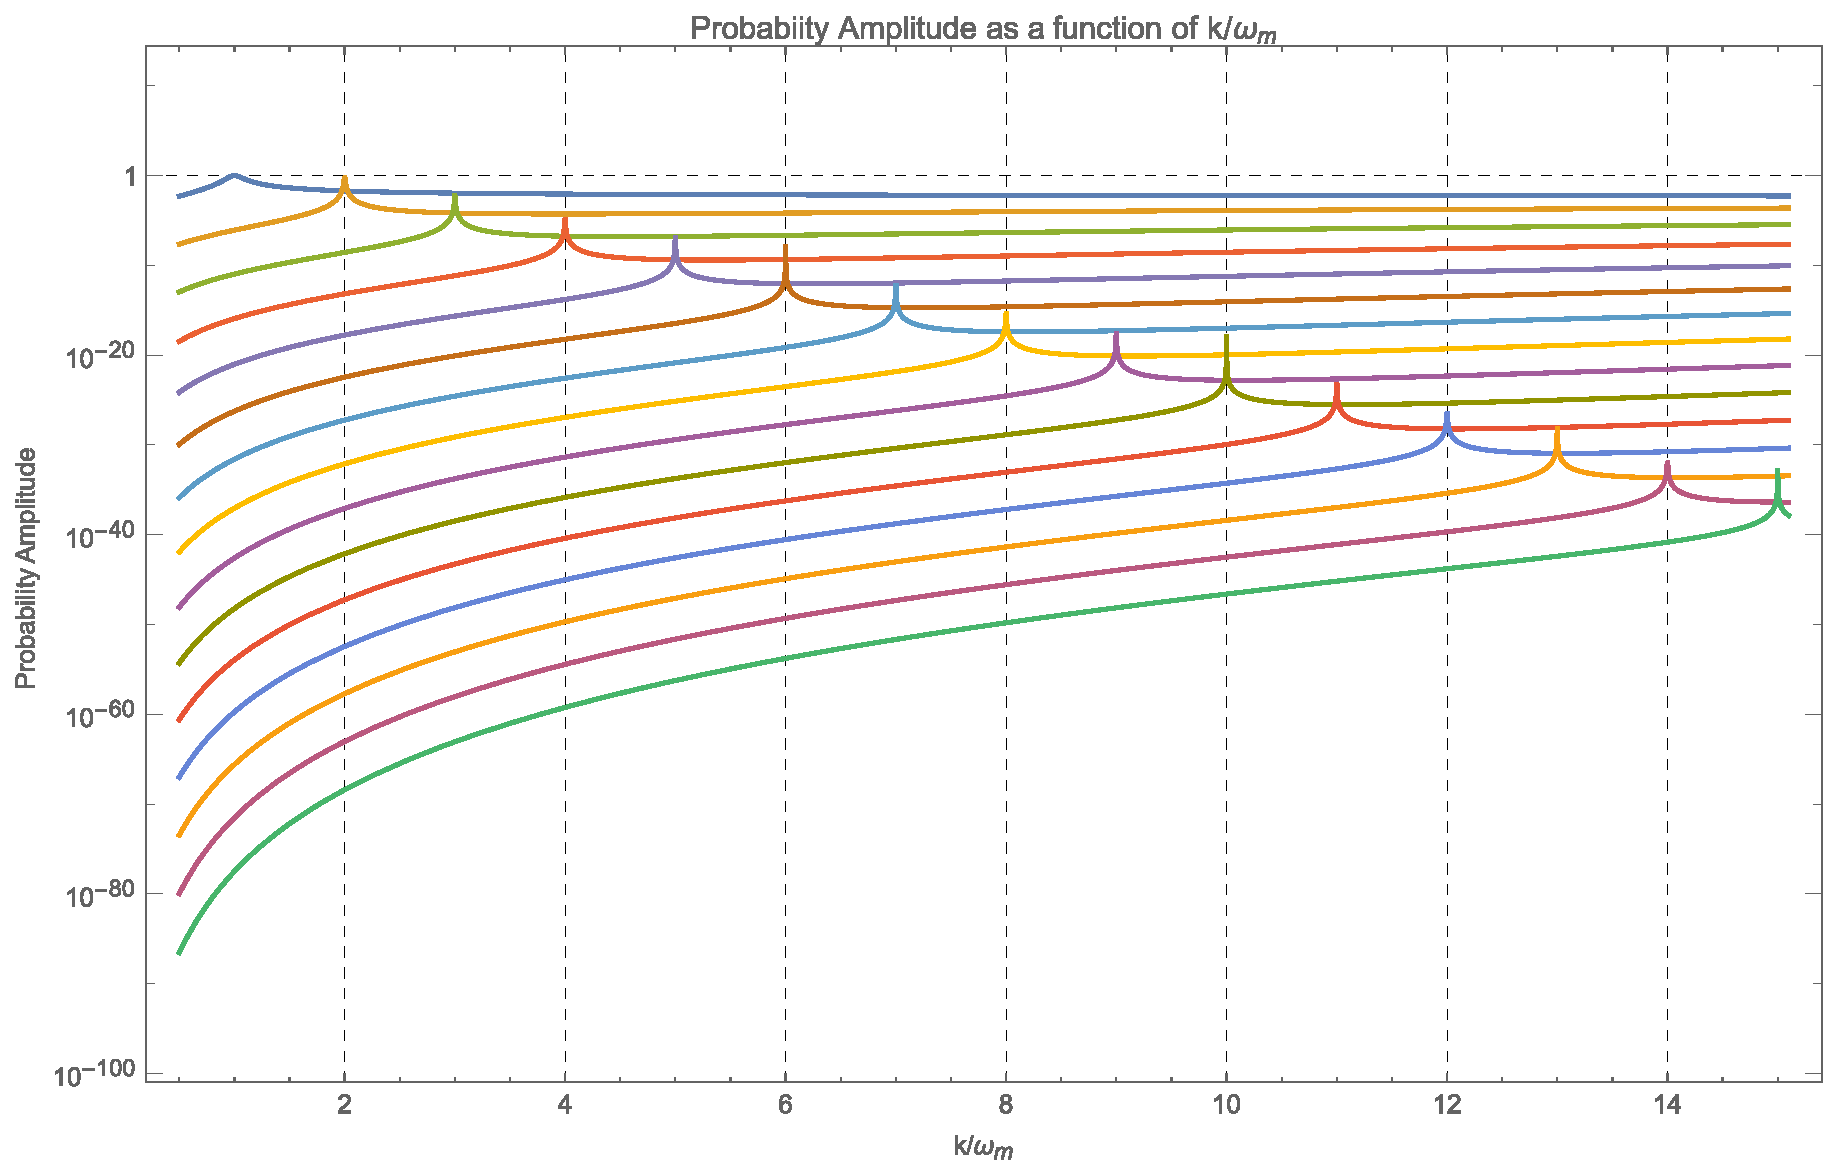
\includegraphics[width=\textwidth]{chapters/assets/rabi/stimulated-probability-apmlitude-vs-k-Jacobi-Anger.pdf}
    \caption{Probability amplitude as a function of $k/\omega_{\mathrm m}$ for each term in Jacobi-Anger expansion, with parameters $\lambda_1=0.1$,$\theta_{\mathrm m}=\pi/5$.}
    \label{chap:matter-sec:single-revisted-fig:prob-amp-jacobi-anger}
\end{figure}


\begin{figure}[!htbp]
    \centering
    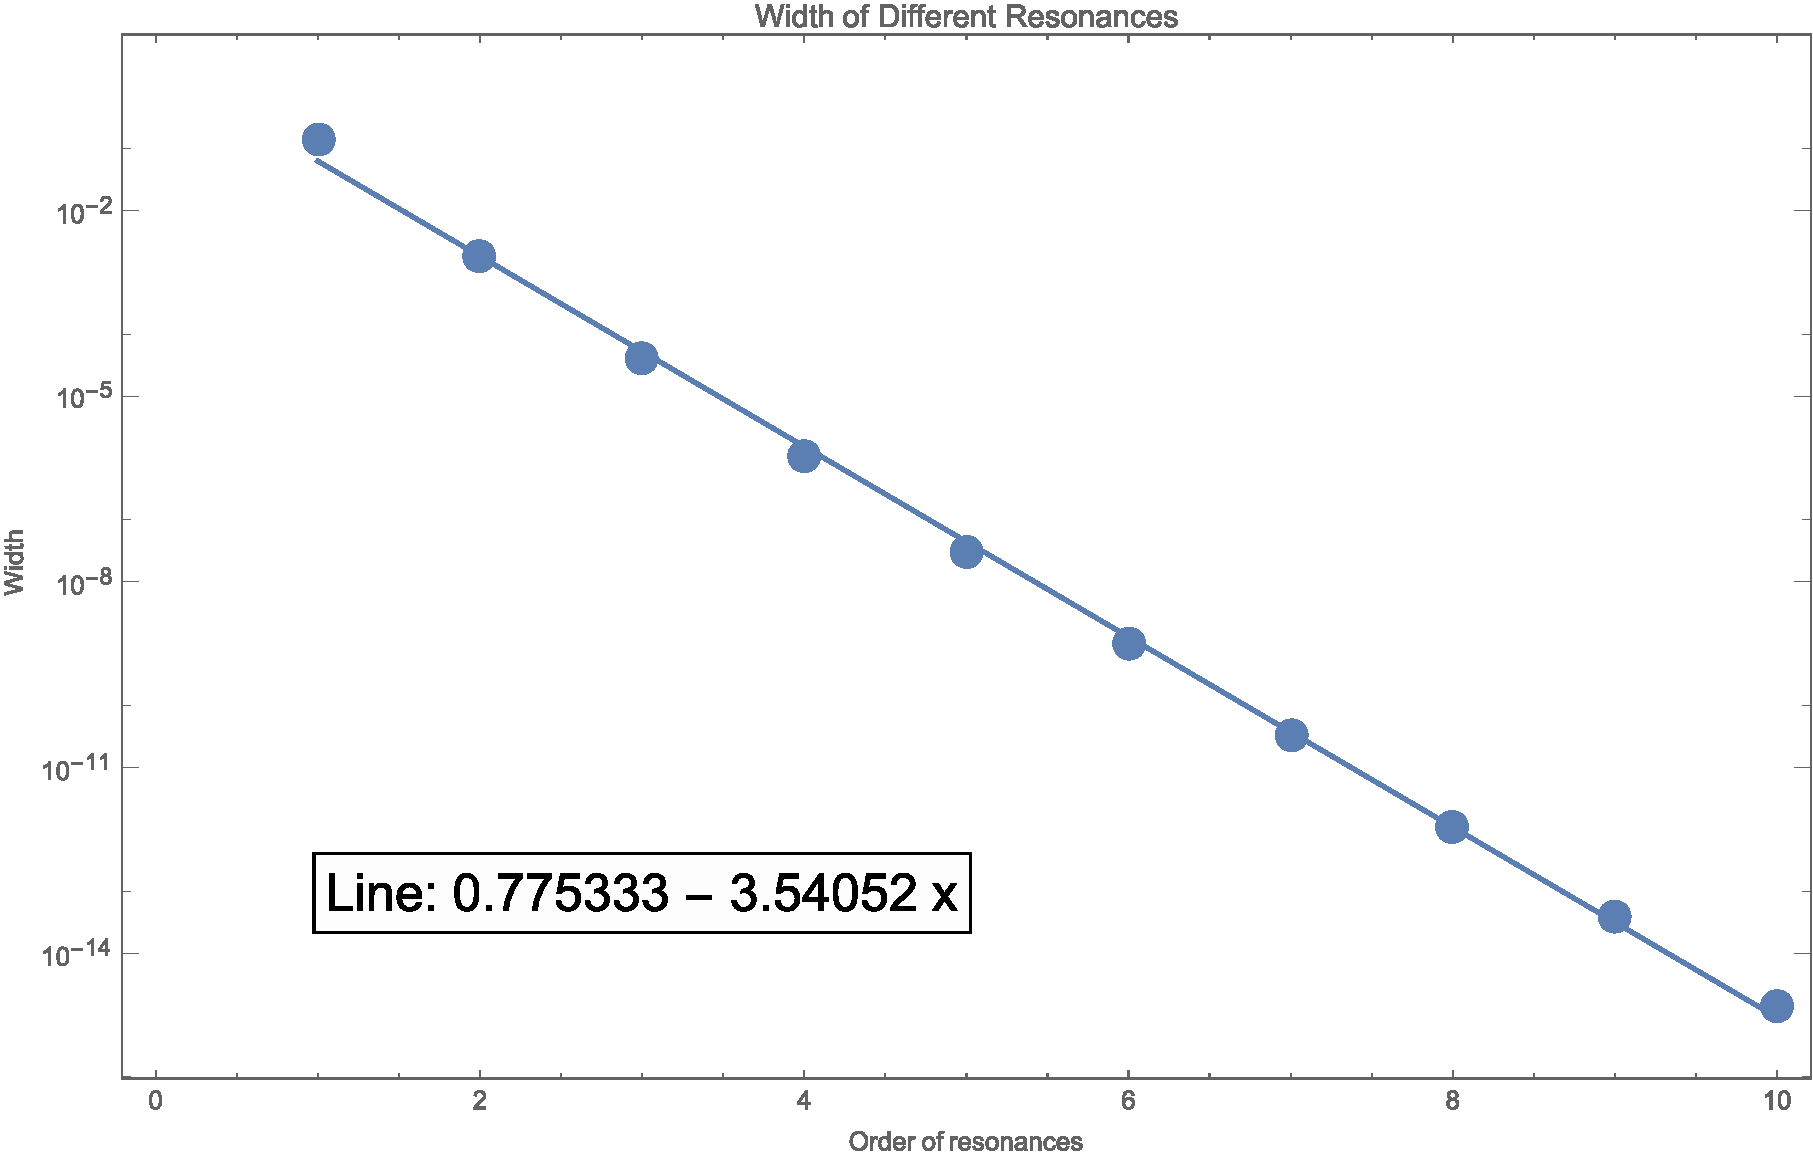
\includegraphics[width=\textwidth]{chapters/assets/rabi/stimulated-probability-apmlitude-vs-k-resonance-width.pdf}
    \caption{Resonance width as a function of mode order for each term in Jacobi-Anger expansion, with parameters $\lambda_1=0.1$,$\theta_{\mathrm m}=\pi/5$.}
    \label{chap:matter-sec:single-revisted-fig:resonance-width-jacobi-anger-exp}
\end{figure}



\begin{figure}[!htbp]
    \centering
    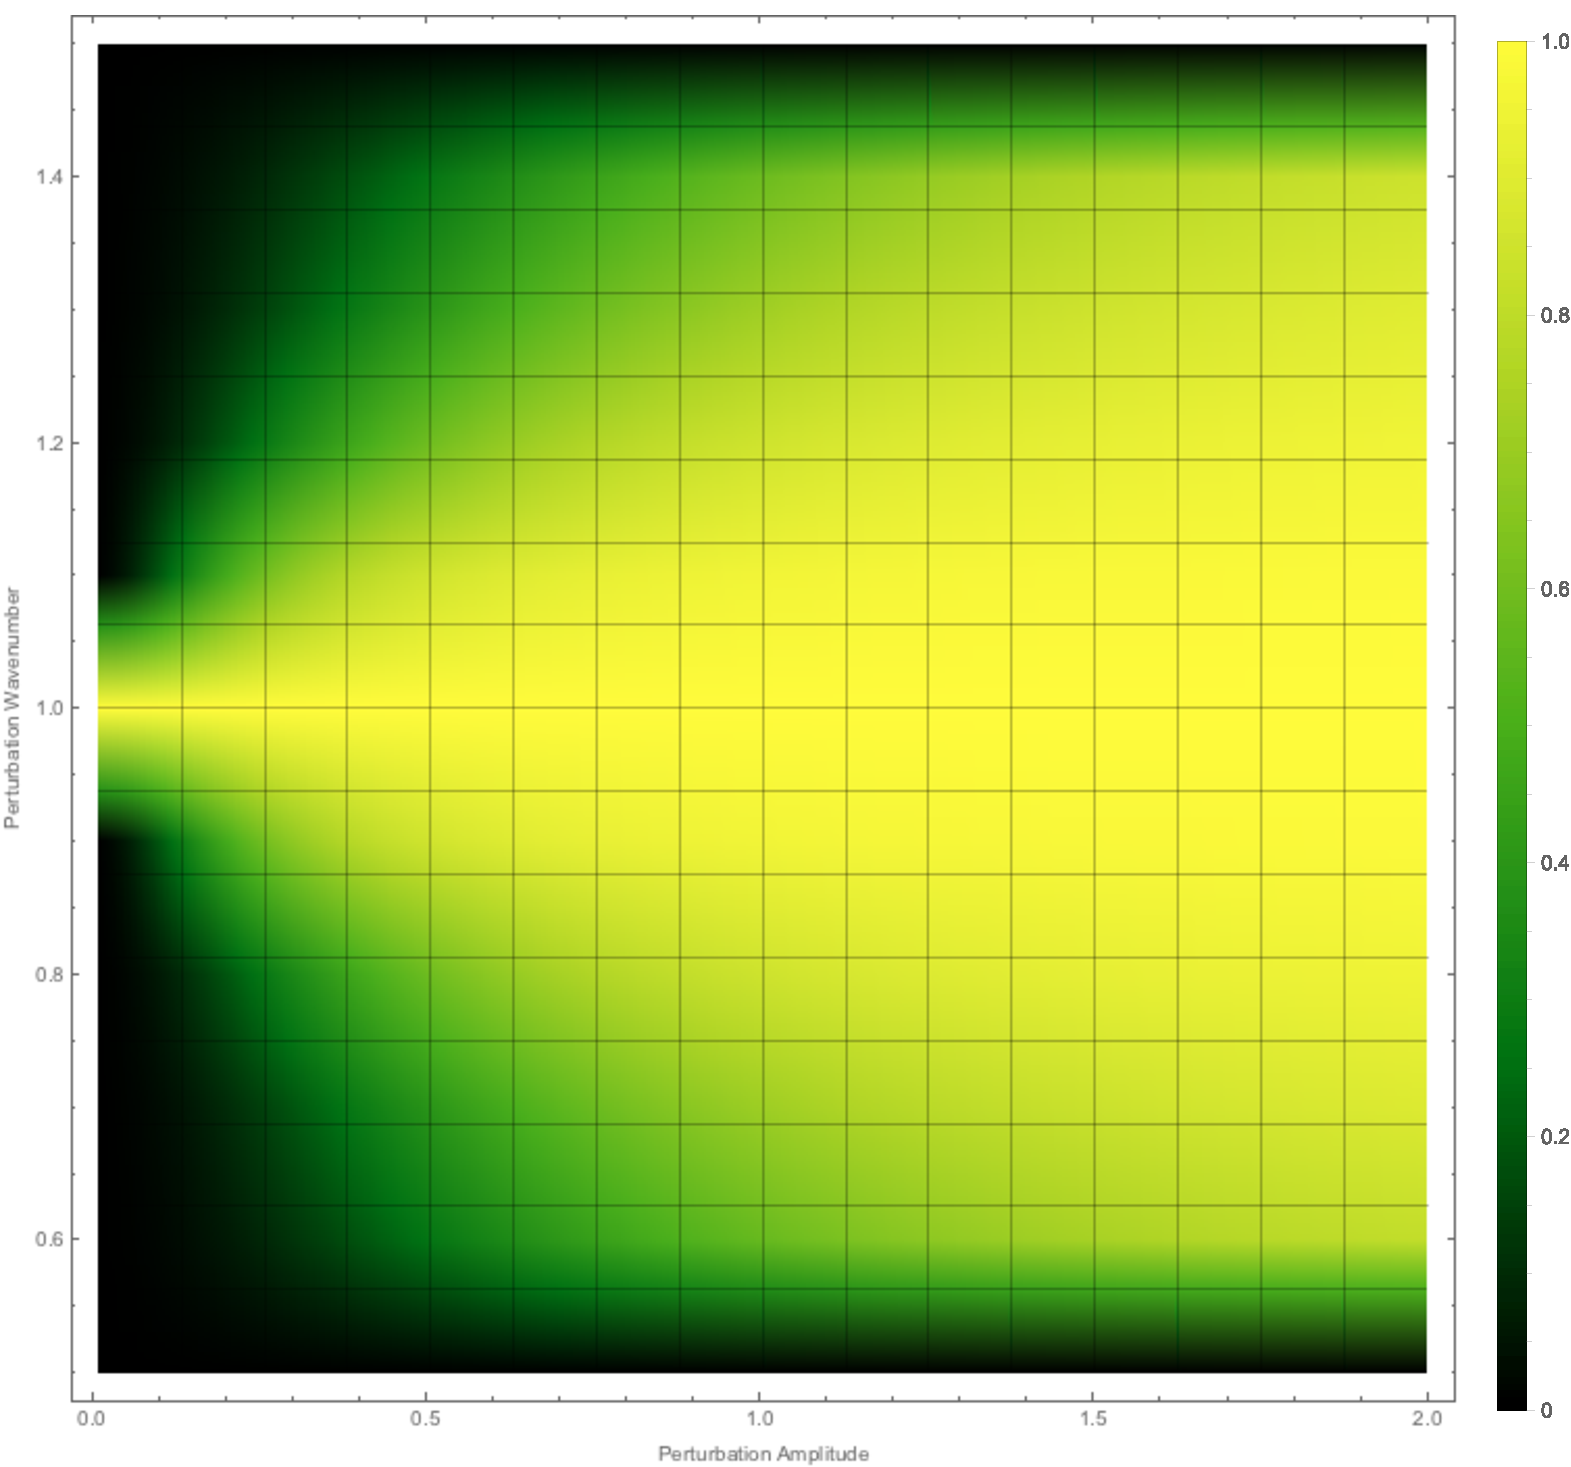
\includegraphics[width=\textwidth]{chapters/assets/rabi/pltPertAmpPertWaveNumTransitionAmp}
    \caption{Transition probability amplitude at different perturbation amplitude and perturbation wavenumber. Larger amplitudes corresponds to larger resonance width, as another confirmation to Fig.~\ref{chap:matter-sec:single-revisted-fig:resonance-width-jacobi-anger-exp}.}
    \label{chap:matter-sec:single-revisted-fig:resonance-width-heatmap}
\end{figure}





\subsection{Castle Wall Matter Profile}



For completeness of this chapter, we show one example of multi-frequency matter profile. One of the multi-frequency matter profiles that has been well studied is the castle wall matter profile. Using Fourier series, any matter profile can be Fourier decomposed into superposition of many single frequency matter profile in principle. We decompose the periodic castle wall matter profile into many frequencies and study the interference effect. The potential shown in Fig.~\ref{fig-castlewall-profile-illustration} is defined as,
\begin{equation}
    \lambda(r) = \begin{cases}
\Lambda_1, &\quad -\frac{X_1}{2}+nX\le r\le \frac{X_1}{2}+nX \\
\Lambda_2, &\quad \frac{X_1}{2}+nX\le r\le \frac{X_1}{2}+\frac{X_2}{2} +nX
\end{cases}
\label{eq-castle-wall-potential}
\end{equation}
where $X_1$ and $X_2$ are the two periods of the matter profile or potential, $X=X_1+X_2$, and $n$ is integer. The parametric resonance condition derived by E. Akhmedov~\cite{Akhmedov2000} is,
\begin{equation}
    \frac{\tan (\omega_{\mathrm m1}X_1/2)}{\tan (\omega_{\mathrm m2}X_2/2)} = - \frac{\cos 2\theta_{\mathrm m2}}{\cos 2\theta_{\mathrm m1}},
    \label{eq-akhmedov-resonance-condition-castle-wall}
\end{equation}
where $\omega_{\mathrm{m}i}$ and $\theta_{\mathrm{m}i}$ are the energy difference and mixing angle for potential $\Lambda_1$ and $\Lambda_2$ respectively.

Even though this castle wall problem is analytically solved, the resonance condition Eqn.~(\ref{eq-akhmedov-resonance-condition-castle-wall}) itself is not transparent. In this subsection, we show that such a system is closed related to Rabi oscillations. For illustration purpose, we set the profile to be equal period for the two densities so that $X_1=X_2\equiv X/2$. To show that the neutrino flavor conversions in this castle wall matter profiles is related to Rabi oscillation, we decompose the profile using Fourier series,
\begin{equation}
\lambda(r) = \lambda_0 + \sum_{n=1}^{\infty} \lambda_n \cos\left( k_n  r \right),
\label{eq-castle-wall-fourier-expanded}
\end{equation}
where
\begin{align*}
\lambda_0 &= (\Lambda_1 + \Lambda_2)/2, \\
\lambda_n & = \frac{2}{(2n-1)\pi}  (-1)^n  \left( \Lambda_1 -  \Lambda_2 \right),\\
k_n &= (2n-1)k_0, \\
k_0 &= 2\pi/X.
\end{align*}
The decomposition is visualized in Fig.~\ref{app-chap:convention-sec:fourier-series-eqn:parametric-resonance-castle-wall-fourier-coeff-even}.

To calculate the transitions between two mass states of background matter potential $\lambda_0$, we use the background matter basis with respect to $\lambda_0$, in which the transition is zero when varying matter profile vanishes. The Hamiltonian
\begin{equation}
H^{(\mathrm m)} = - \frac{1}{2}\omega_{\mathrm m} \sigma_3  + \frac{1}{2} \sum_{n=1}^{\infty} \lambda_n \cos 2\theta_{\mathrm m} \cos\left( k_n  r \right)  \sigma_3 - \frac{1}{2} \sum_{n=1}^{\infty} \lambda_n \sin 2\theta_{\mathrm m}  \cos\left( k_n r \right) \sigma_1,
\label{castle-wall-decomposed-hamiltonian}
\end{equation}
determines the transitions between the two background matter states.


\begin{figure}[!htbp]
    \centering
    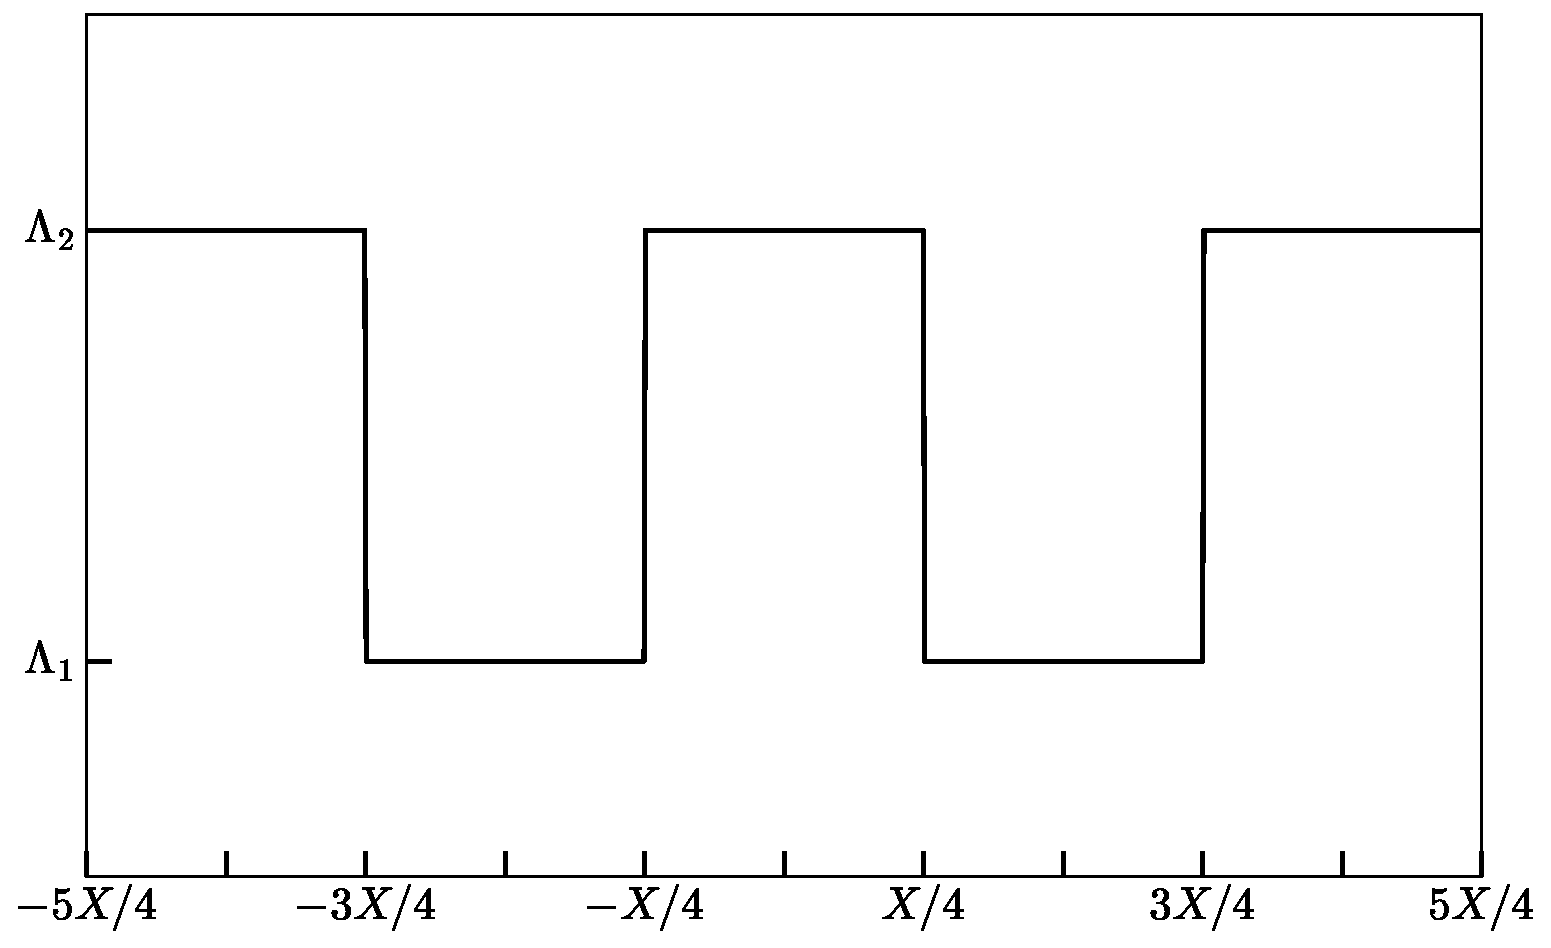
\includegraphics[width=\columnwidth]{chapters/assets/rabi/castlewall-profile}
    \caption{The castle wall matter potential profile with $X_1=X_2=X/2$.}
    \label{fig-castlewall-profile-illustration}
\end{figure}



% \begin{figure}[!htbp]
%     \centering
%     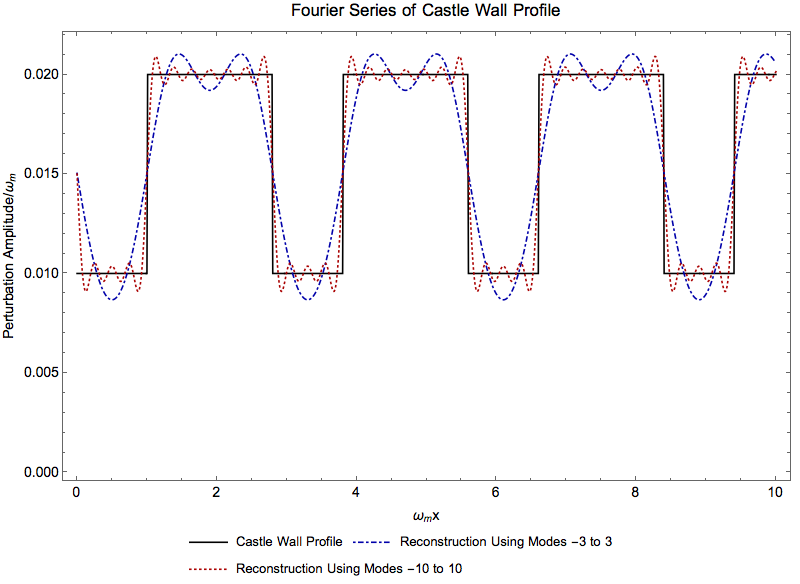
\includegraphics[width=\textwidth]{chapters/assets/rabi/reconstruction-of-castle-wall-0point01-0point02-1-1point8}
%     \caption{Decomposition of castle wall density profile using Fourier modes.}
%     \label{chap:matter-sec:castlewall-fig:decompose-castlewall-fourier}
% \end{figure}


\begin{figure}[!htbp]
        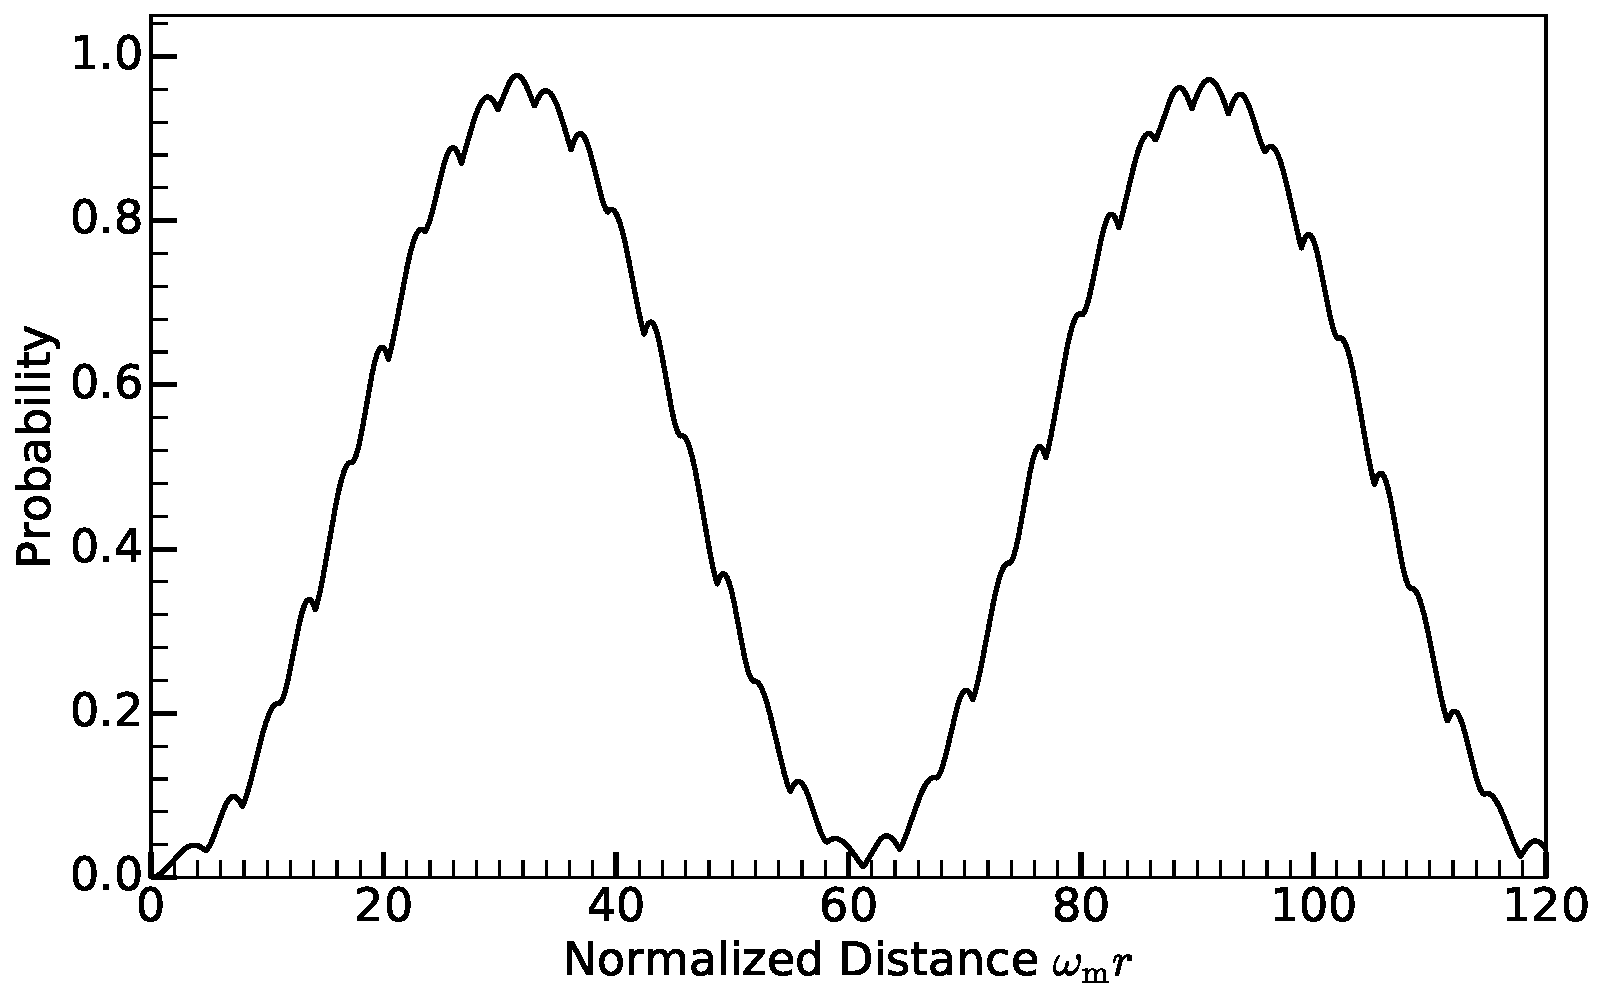
\includegraphics[width=\columnwidth]{chapters/assets/rabi/castle-wall-1}%
    \caption{Transition probabilities for castle wall matter profile calculated numerically for $\Lambda_2-\Lambda_1=0.4 \Lambda_0$. During the calculation, the energy of neutrinos is $10\,\mathrm{MeV}$, mass-squared difference is $\delta m^2=2.6\times 10^{-3}\,\mathrm{eV^2}$, and the vacuum mixing angle chosen so that $\sin^2(2\theta_\vv)=0.093$. The background potential $\Lambda_0$ is chosen so that it's half the MSW resonance potential, $\Lambda_0 = \frac{1}{2}\lambda_{\mathrm{MSW}}=\frac{1}{2}\omega_{\mathrm{v}}\cos 2\theta_{\mathrm v}$, and the base frequency is set to $k_0 = 2\pi/X = \omega_{\mathrm{m}}$.
                 }
    \label{fig-akhmedovOscPlt}
\end{figure}


In principle, the base frequency $k_0$ which is determined by the total period $X$ can be arbitrary. In this example, we choose a $X$ so that the base frequency $k_0$ matches the energy gap $\omega_{\mathrm{m}}$. Even though multiple perturbation frequencies show up in Eqn.~(\ref{castle-wall-decomposed-hamiltonian}), we identify that only the first frequency $n=1$ is the resonance frequency since we are using $k_0=\omega_{\mathrm{m}}$. As an approximation, we drop all other frequencies $n>2$ regarding the fact that they are far from resonance. Thus, similar to single frequency matter profile, the varying $\sigma_3$ terms have limited effects on the transition probabilities in our case, which leads to
\begin{align*}
    H^{(\mathrm m)} \to & - \frac{1}{2}\omega_{\mathrm m} \sigma_3  - \frac{1}{2} \sum_{n=1}^2\lambda_n \sin 2\theta_{\mathrm m}  \cos\left( k_n r \right) \sigma_1\\
    \to & - \frac{1}{2}\omega_{\mathrm m} \sigma_3  - \frac{1}{2} \sum_{n=1}^2 A_n \cos ( k_n r) \sigma_1 \\
    & + \frac{1}{2} \sum_{n=1}^2A_n \sin(k_n r) \sigma_2,
\end{align*}
where
\begin{equation*}
A_n = \frac{\lambda_n \sin 2\theta_{\mathrm m} }{2} .
\end{equation*}
The relative detuning is $0$ if we have only the first mode. However, it becomes
\begin{equation}
\RD_1'= \frac{A_2^2}{2\lvert A_1 (\omega_{\mathrm m} - k_2) \rvert},
\end{equation}
if we include the second frequency $k_2$. One feature of this Fourier series expanded matter profile Eqn.~(\ref{eq-castle-wall-fourier-expanded}) is that the width of each frequency decreases as the order $n$ increases while the detuning of each frequency increases. We calculate the relative detuning for each frequency
\begin{equation}
\RD_n = \frac{\lvert k_n -\omega_{\mathrm m} \rvert}{ \lvert \lambda_n  \sin 2\theta_{\mathrm m}/2 \rvert } = \frac{2(n-1)(2n-1)\pi \omega_{\mathrm m}}{(\Lambda_2 - \Lambda_1)\sin 2\theta_{\mathrm m}}
\end{equation}
which is quadratic in $n$ and inversely proportional to $\Lambda_2-\Lambda_1$. We find that all higher frequencies $k_n$ for $n>2$ have very large relative detunings. The neutrino transition probability between the two matter states is shown in Fig.~\ref{fig-akhmedovOscPlt}, where we find the system has almost full transition.

A more rigorous treatment is to use Jacobi-Anger expansion and find the Rabi modes, where we find that the mode that corresponds to single frequency $k_1$ dominates and all other modes have little destruction effect on it. Quantitatively, higher orders leads to smaller width $B_{\{n_i\}}$ yet larger detuning $\sum_{n} nk_n-\omega_{\mathrm m}$, which renders a smaller effect on the resonance mode $\{1,0\}$, since the effect is evaluated as Eqn.~(\ref{eq-relative-detuning-changed}).
Table~\ref{tab-q-values-each-mode} lists the first few smallest relative detunings of Fig.~\ref{fig-akhmedovOscPlt}. The second column is the relative detuning of the corresponding mode, while the third column is the relative detuning of mode $\{1,0\}$ with the energy gap shift effect of the corresponding mode.



% Find the data in MMA file `akhmedov-parametric-resonance.nb`
% {0., 6129.81, 20432.7, 42908.7}
% {0., 5.99981, 19.9994, 41.9987}

\begin{table}
\centering

% \begin{ruledtabular}
\begin{tabular}{lll}
\hline
 $\{n_1,n_2\}$ &  $\RD$ & $\RD'_{\{1,0\}}$   \\
\hline
 $\{1,0\}$ & $0$ &  - \\
 $\{-1,0\}$ & $48$ &  $1.0\times 10^{-2}$ \\
 $\{0,1\}$ & $1.5\times 10^2$ &  $1.1\times 10^{-3}$  \\
 $\{2,0\}$ & $2.4\times 10^{2}$ & $2.0\times 10^{-4}$ \\
 \hline
\end{tabular}
% \end{ruledtabular}
\caption{\label{tab-q-values-each-mode}Relative detuning of each frequency.}
\end{table}


\section{\label{chap:matter-sec:deep-jacobi}Deep Diving into Jacobi-Anger Expansion}


\subsection{\label{chap:matter-sec:deep-jacobi-subsec:single-matter-freq}Single Matter Density Frequencies}

As a first step, we solve single frequency matter perturbation
\begin{equation}
   \delta \lambda(x)  = A \sin (k x + \phi).
\end{equation}

Using the relation between $\eta$ and $\delta\lambda$, we solve out $\eta$.
\begin{equation}
   \eta(x) = - \frac{\omega_\mm}{2}x - \frac{\cos 2\theta_\mm}{2} \frac{A}{k} \cos (k x + \phi),
\end{equation}
where we have chosen $\eta(0)=-\frac{\cos 2\theta_\mm}{2}\frac{A}{k}\cos\phi$.
The problem is to solve the equation of motion
\begin{equation}
   i \frac{d}{dx} \begin{pmatrix} \psi_{b1} \\ \psi_{b2} \end{pmatrix} = \frac{\sin 2\theta_\mm}{2}\delta\lambda(x) \begin{pmatrix} 0 &  e^{2i\eta(x)} \\   e^{-2i\eta(x)} &  0 \end{pmatrix}  \begin{pmatrix} \psi_{b1} \\ \psi_{b2} \end{pmatrix} .
\end{equation}
We also define
\begin{align}
   h &= \frac{\sin 2\theta_\mm}{2}\delta\lambda(x)  e^{2i\eta(x)} \\
   & = \frac{\sin 2\theta_\mm}{2} A \sin (kx+\phi) e^{i\left( -\omega_\mm x - \frac{A \cos 2\theta_\mm}{k} \cos (kx+\phi) \right)},
   \label{chap:matter-sec:deep-jacobi-subsec:single-matter-freq-eqn:single-frequency-hamiltonian-element}
\end{align}
so that the equation of motion becomes
\begin{equation}
   i \frac{d}{dx} \begin{pmatrix} \psi_{b1} \\ \psi_{b2} \end{pmatrix} =  \begin{pmatrix} 0 &  h \\   h^* &  0 \end{pmatrix}  \begin{pmatrix} \psi_{b1} \\ \psi_{b2} \end{pmatrix} .
\end{equation}
We apply Jacobi-Anger expansion, c.f.~Eqn.~\ref{eqn:jacobi-anger-expansion}, to rewrite the exponential into some plane wave terms~\cite{Patton2014}.

We define $z_k = \frac{A}{k} \cos 2\theta_\mm$, with which we expand the term
\begin{equation}
   e^{-i\frac{\cos 2\theta_\mm A}{k} \cos (kx +\phi)} = \sum_{n=-\infty}^\infty i^n J_n (-z_k) e^{in (kx +\phi)} =  \sum_{n=-\infty}^\infty (-i)^n J_n (z_k) e^{in (kx +\phi)},
\end{equation}
where I used $J_n(-z_k) = (-1)^n J_n(z_k)$ for integer $n$.
The expansion is plugged into the Hamiltonian elements,
\begin{align}
   h &= \frac{A \sin 2\theta_\mm \sin (kx + \phi)}{2} e^{-i\omega_\mm x } \sum_{n = - \infty}^\infty (-i)^n J_n(z_k) e^{i n ( kx + \phi)} \\
   & = \frac{A\sin 2\theta_\mm}{4i} \left( e^{i(kx + \phi)} - e^{-i(kx+\phi)} \right) e^{-i\omega_\mm x } \sum_{n = - \infty}^\infty (-i)^n J_n(z_k) e^{i n ( kx + \phi)} \\
   & = \frac{A\sin 2\theta_\mm}{4i} \left( \sum_{n=-\infty}^\infty e^{i(n+1)} i^n J_n (z_k) e^{i((n+1) k - \omega_\mm)x}  - \sum_{n'=-\infty}^\infty e^{i(n'-1)} (-i)^{n'}J_{n'}(z_k) e^{i( (n'-1)k - \omega_\mm)x}  \right)\\
   & = \frac{A\sin 2\theta_\mm}{4} \sum_{n=-\infty}^{\infty} e^{in\phi} \left( - (-i)^n \right) \frac{2n}{z_k} J_n (z_k) e^{i(nk-\omega_\mm)x},
\end{align}
where I have used
\begin{equation}
   J_{n-1}(z_k) + J_{n+1}(z_k) = \frac{2n}{z_k} J_n(z_k).
\end{equation}

Here comes the approximation. The most important oscillation we need is the one with largest period, which indicates the phase to be almost zero,
\begin{align}
   (n+1) k -\omega_\mm &\sim 0 \\
   (n'-1) k -\omega_\mm &\sim 0.
   \label{chap:matter-sec:deep-jacobi-subsec:single-matter-freq-eqn:single-frequency-rwa-requirement}
\end{align}

The two such conditions for the two summations are
\begin{align}
   n \equiv n_- &= \mathrm{Int}\left( \frac{\omega_\mm}{k} \right) - 1 \\
   n' \equiv n_+ &= \mathrm{Int}\left( \frac{\omega_\mm}{k} \right) + 1 .
\end{align}
We define $\mathrm{Int}\left( \frac{\omega_\mm}{k} \right) = n_0$,
\begin{align}
   n_- &= n_0 - 1 \\
   n_+ &= n_0 + 1 .
\end{align}

The element of Hamiltonian is written as
\begin{equation}
   h = - \frac{A\sin 2\theta_\mm}{2} e^{in_0\phi} (-i)^{n_0} \frac{n_0}{z_k} J_{n_0 }(z_k) e^{i(n_0 k -\omega_\mm)x}.
\end{equation}

To save keystrokes, we define
\begin{equation}
   F = - A\sin 2\theta_\mm e^{i n_0 \phi} (-i)^{n_0} \frac{n_0}{z_k} J_{n_0} (z_k) ,
   \label{chap:matter-sec:deep-jacobi-subsec:single-matter-freq-eqn:definition-F}
\end{equation}
which depends on $n_0$ and $z_k = \frac{A}{k} \cos 2\theta_\mm$. Notice that
\begin{equation}
   \lvert F \rvert^2 = \left\lvert  k \tan 2\theta_\mm  n_0 J_{n_0} (z_k) \right\rvert^2 .
\end{equation}
Thus the 12 element of the Hamiltonian is rewritten as
\begin{equation}
   h = \frac{1}{2}F e^{i(n_0 k -\omega_\mm)x}.
   \label{chap:matter-sec:deep-jacobi-subsec:single-matter-freq-eqn:eqn-12-element-and-F}
\end{equation}

% .. admonition:: Solving Using Mathematica
%   :class: hint

%   The Mathematica code::

%       In[1]:= sys = I D[{phi1[x], phi2[x]}, x] == {{0, (g0R + I g0I) Exp[ I (-omegam + n0 k) x]}, {(g0R - I g0I) Exp[-I (-omegam + n0 k) x], 0}}.{phi1[x], phi2[x]}
%       In[2]:= DSolve[sys, {phi1, phi2}, x]// FullSimplify
%       Out[3]:= {{phi1 -> Function[{x},
%       E^(1/2 I (k n0 + I Sqrt[-4 (g0I^2 + g0R^2) - (k n0 - omegam)^2] - omegam) x) C[1]
%       + E^(1/2 (Sqrt[-4 (g0I^2 + g0R^2) - (k n0 - omegam)^2] + I (k n0 - omegam)) x) C[2]],
%       phi2 -> Function[{x}, (1/(2 (g0I - I g0R)))
%       I E^(-I (k n0 - omegam) x +
%       1/2 I (k n0 + I Sqrt[-4 (g0I^2 + g0R^2) - (k n0 - omegam)^2] - omegam) x)
%       (k n0 + I Sqrt[-4 (g0I^2 + g0R^2) - (k n0 - omegam)^2] - omegam) C[1]
%       + (1/(2 (g0I - I g0R))) E^(1/2 (Sqrt[-4 (g0I^2 + g0R^2) - (k n0 - omegam)^2]
%       + I (k n0 - omegam)) x - I (k n0 - omegam) x) (Sqrt[-4 (g0I^2 + g0R^2) - (k n0 - omegam)^2]
%       + I (k n0 - omegam)) C[2]]}}



The general solution to the equation of motion is
\begin{align}
   \psi_{b1} = & C_1 e^{\frac{1}{2} i \left( n_0 k -\omega_\mm - \sqrt{  \lvert F \rvert^2 +  (n_0 k -\omega_\mm)^2 } \right)x} + C_2 e^{\frac{1}{2} i \left( n_0 k -\omega_\mm + \sqrt{  \lvert F \rvert^2 +  (n_0 k -\omega_\mm)^2 } \right)x} \\
   \psi_{b2} = & \frac{C_1}{F^*} i \left( n_0 k - \omega_\mm - \sqrt{ \lvert F\rvert^2 + ( n_0 k - \omega_\mm )^2 } \right) e^{ -\frac{1}{2}i (n_0 k - \omega_\mm ) x - \frac{1}{2} i \sqrt{ \lvert F \rvert^2 + (n_0 k - \omega_\mm )^2 }  } \nonumber\\
   & + \frac{C_2}{F^*} i \left( n_0 k - \omega_\mm + \sqrt{ \lvert F\rvert^2 + ( n_0 k - \omega_\mm )^2 }  \right)   e^{ -\frac{1}{2}i (n_0 k - \omega_\mm ) x + \frac{1}{2} i \sqrt{ \lvert F \rvert^2 + (n_0 k - \omega_\mm )^2 }  } .
\end{align}
For simplicity, we define
\begin{align}
   g &= n_0 k  - \omega_\mm, \\
   q^2 &= \lvert F \rvert^2 + g^2.
   \label{chap:matter-sec:deep-jacobi-subsec:single-matter-freq-eqn:definition-g-q}
\end{align}

To determine the constants, we need initial condition,
\begin{equation}
   \begin{pmatrix} \psi_1 (0) \\ \psi_2(0)  \end{pmatrix} = \begin{pmatrix} 1 \\ 0  \end{pmatrix} ,
\end{equation}
which leads to
\begin{equation}
   \begin{pmatrix} \psi_{b1} (0) \\ \psi_{b2}(0)  \end{pmatrix} = \begin{pmatrix} e^{i\eta(0)} \\ 0  \end{pmatrix}.
\end{equation}
% using equation :ref:`wavefunction in background matter basis <matter-stimulated-equation-wavefunction-diff-basis>`.

Plug in the initial condition for the wave function,
\begin{align}
   C_1 + C_2 &= e^{i \frac{z_k}{2}\cos \phi} \\
   \frac{C_1}{2F^ * } i \left( g - q \right) + \frac{C _ 2}{ F ^ *} i \left( q + g  \right) & = 0.
\end{align}
The constants are solved out
\begin{align}
   C_1 &= e^{i \frac{z_k}{2}\cos \phi} \frac{q + g }{2 q} , \\
   C_2 &= e^{i \frac{z_k}{2}\cos \phi} \frac{ q - g }{2 q}.
\end{align}
where $F$ is defined in \ref{chap:matter-sec:deep-jacobi-subsec:single-matter-freq-eqn:definition-F} and $l$ and $g$ are defined in \ref{chap:matter-sec:deep-jacobi-subsec:single-matter-freq-eqn:definition-g-q}.
The second element of wave function becomes
\begin{equation}
   \psi_{b2}(x) = \frac{- F}{ q } e^{i\frac{z_k}{2} \cos\phi} e^{- \frac{i}{2}gx} \sin \left( \frac{1}{2} q x \right).
\end{equation}

The transition probability becomes
\begin{equation}
   P_{1\to 2} = \lvert \psi_{b2} \rvert^2 = \frac{\lvert F \rvert^2}{q^2} \sin^2\left( \frac{ q }{2} x \right),
\end{equation}
where $q$ is the oscillation wavenumber. Period of this oscillation is given by $T = \frac{2\pi}{q}$.

Compared to the results by Kneller et al~\cite{Kneller2013}, where the transition probability is
\begin{equation}
    {\color{red}P_{12} = \frac{\kappa_n^2}{q_n^2} \sin^2 (q_n x)},
\end{equation}
where $\color{red}q_n^2 = k_n^2 + \kappa_n^2$ and $\color{red}2k_n = \tilde{\delta k}_{12} + n k_\star$.

In my notation, $k$ is the same as their $\color{red}k_\star$. After the first step of translation, we have $g = \color{red} 2 k_n$.

The definition of $\color{red}\kappa_n$ is given by
\begin{equation}
    {\color{red}\kappa_{ij,n} = (-i)^{n-1} \frac{n C_\star V_\star}{z_{ij}} J_n(z_{ij}) \tilde U_{ei}^* \tilde U_{ej} e^{i ( n \eta + z_{ij} \cos \eta)} },
\end{equation}
in Kneller et al's notation and
\begin{equation}
  \delta V_{ee}(x) = C_\star V_\star \sin (k_\star x + \eta).
\end{equation}
So we conclude that my $\lvert F \rvert ^2$ is related to Kneller et al's $\lvert \kappa_n \rvert^2$ through
\begin{equation}
  \lvert F \rvert^2 = 4 {\color{red} \lvert \kappa_n \rvert^2}.
\end{equation}
We also have
\begin{equation}
  q^2 = \lvert F \rvert ^2 + g^2  = 4 {\color{red} q_n^2},
\end{equation}
i.e., ${\color{red}q_n} = \frac{ q }{2}$.
Now we see the method we have used gives exactly the same transition probability as Kneller et al's.


To make the numerical calculations easier, we rewrite the result by defining the scaled variables
\begin{align}
   \hat x & = \omega_\mm x,\\
   \hat k &= \frac{k}{\omega_\mm}, \\
   \hat A & = \frac{A}{\omega_\mm}, \\
   \hat g & = \frac{g}{\omega_\mm} = n_0 \hat k - 1,\\
   \hat q &= \sqrt{ \lvert \hat F \rvert^2 + \hat g^2 } = \sqrt{ \lvert \hat k \tan 2\theta_\mm n_0 J_{n_0} (z_k) \rvert + \hat g^2 },
\end{align}
so that $n_0 = \mathrm{Round}\left( 1/\hat k\right)$, $z_k=\frac{\hat A}{\hat k} \cos 2 \theta_\mm$ and
\begin{equation}
   P_{1\to 2} = \frac{\left\lvert \hat k \tan 2\theta_\mm n_0 J_{n_0} (z_k) \right\rvert^2}{\left\lvert  \hat k \tan 2\theta_\mm n_0 J_{n_0} (z_k) \right\rvert^2 + \hat g ^2}\sin^2\left( \frac{ \hat q }{2} \hat x \right) .
   \label{chap:matter-sec:deep-jacobi-subsec:single-matter-freq-eqn:stimulated-single-freq-trans-probability}
\end{equation}



\subsubsection{Mathematical Analysis of The Result}


There are several question to answer before we can understand the picture of the math.
\begin{itemize}
    \item What does each term mean in the Hamiltonian?
\item What exactly is the unitary transformation we used to rotate the wave function?
\item What is the physical meaning of Jacobi-Anger expansion in our calculation?
\end{itemize}

To answer the first question, we need to write down the solution to Schrodinger equation assuming the Hamiltonian has only one term. The results are listed below in Table~\ref{chap:matter-sec:deep-jacobi-subsec:single-matter-freq-tab:decomp-hamil}.

\begin{table*}
\centering
% \begin{ruledtabular}
% \small
\setlength\tabcolsep{2pt}
\begin{tabular}{l|l}
\hline
 Hamiltonian &   Solution to The First Element of Wave Function \\
\hline
   $-\frac{\omega_\mm}{2}\sigma_3$ &  $\psi_1 \sim e^{i\omega_\mm x/2}$  \\
   $\frac{\delta\lambda}{2}\cos 2\theta_\mm \sigma_3$     &   $\psi_1 \sim e^{i\frac{A\cos 2\theta_\mm}{2k}\cos(kx+\phi)}$ \\
  $\frac{\delta\lambda}{2}\cos 2\theta_\mm \sigma_3$     &   $\psi_1 = C_1 e^{i\frac{A\sin 2\theta_\mm}{2k}\cos(kx+\phi)} + C_2 e^{-i\frac{A\sin 2\theta_\mm}{2k}\cos(kx+\phi)}$ \\
\hline

\end{tabular}
% \end{ruledtabular}
\caption{\label{chap:matter-sec:deep-jacobi-subsec:single-matter-freq-tab:decomp-hamil}Each terms in Hamiltonian and the corresponding solutions to the specific term.}
\end{table*}


% ============================================================ =================================================================================================================================
% Hamiltonian                                                       Solution to The First Element of Wave Function
% ============================================================ =================================================================================================================================
% .. math:: -\frac{\omega_\mm}{2}\sigma_3                           .. math:: \psi_1 \sim e^{i\omega_\mm x/2}
% .. math:: \frac{\delta\lambda}{2}\cos 2\theta_\mm \sigma_3        .. math:: \psi_1 \sim e^{i\frac{A\cos 2\theta_\mm}{2k}\cos(kx+\phi)}
% .. math:: \frac{\delta\lambda}{2}\cos 2\theta_\mm \sigma_3        .. math:: \psi_1 = C_1 e^{i\frac{A\sin 2\theta_\mm}{2k}\cos(kx+\phi)} + C_2 e^{-i\frac{A\sin 2\theta_\mm}{2k}\cos(kx+\phi)}
% ============================================================ =================================================================================================================================


The unitary transformation used is to move our reference frame to a co-rotating one. $-\frac{\omega_\mm}{2}\sigma_3$ is indeed causing the wave function to rotate and removing this term using a transformation means we are co-rotating with it. $\frac{\delta\lambda}{2}\cos 2\theta_\mm \sigma_3$ causes a more complicated rotation however it is still a rotation.

As for Jacobi-Anger expansion, it expands an oscillating matter profile to infinite constant matter potentials. To see it more clearly, we assume that $\delta\lambda= \lambda_c$ is constant. After the unitary transformation, the effective Hamiltonian is

\begin{equation}
   H' = \frac{\sin 2\theta_\mm}{2} \lambda_c \begin{pmatrix} 0 & e^{2i\eta(x)} \\ e^{-2i\eta(x)} & 0 \end{pmatrix},
\end{equation}
where $\eta(x) = -\frac{\omega_\mm}{2}x + \frac{\cos 2\theta_\mm}{2}\lambda_c x$ and we have chosen $\eta(0)=0$.
The 12 element of the Hamiltonian becomes
\begin{equation}
   \frac{\sin 2\theta_\mm}{2} \lambda_c e^{2i\eta(x)} = \frac{\sin 2\theta_\mm}{2} \lambda_c e^{2i\left( \frac{\omega_\mm}{2} + \frac{\cos 2\theta_\mm}{2} \lambda_c \right)x} .
\end{equation}
The significance of it is to show that a constant matter profile will result in a simple exponential term. However, as we move on to periodic matter profile, we have a Hamiltonian element of the form
\begin{equation}
   h = \frac{\sin 2\theta_\mm}{2} A \sin (kx+\phi) e^{2i\left( -\frac{\omega_\mm}{2} x + \frac{A \cos 2\theta_\mm}{2k} \cos (kx+\phi) \right)},
\end{equation}
as derived in Eqn.~\ref{chap:matter-sec:deep-jacobi-subsec:single-matter-freq-eqn:single-frequency-hamiltonian-element}. To compare with the constant matter case, we make a table of relevant terms in Hamiltonian, Table~\ref{chap:matter-sec:deep-jacobi-subsec:single-matter-freq-tab:decomp-hamil-2}.

\begin{table*}
\centering
% \begin{ruledtabular}
% \small
\setlength\tabcolsep{2pt}
\begin{tabular}{l|l}
\hline
 Constant Matter Profile $\delta\lambda = \lambda_c$ &   Periodic Matter Profile $\delta\lambda=A\sin (kx+\phi)$ \\
\hline
   $\frac{\sin 2\theta_\mm}{2}\lambda_c e^{i \cos 2\theta_\mm \lambda_c x}$     &   $\frac{A\sin 2\theta_\mm}{4} \sum_{n=-\infty}^{\infty} e^{in\phi} \left( - i^n \right) \frac{2n+1}{z_k} J_n (z_k) e^{i(nk-\omega_\mm)x}$ \\
\hline
\end{tabular}
% \end{ruledtabular}
\caption{\label{chap:matter-sec:deep-jacobi-subsec:single-matter-freq-tab:decomp-hamil-2} Comparison of the off diagonal element of Hamiltonian for constant matter density profile and the periodic matter density profile.}
\end{table*}

% ================================================================================   ========================================================================
% Constant Matter Profile :math:`\delta\lambda = \lambda_c`                           Period Matter Profile :math:`\delta\lambda=A\sin (kx+\phi)`
% ================================================================================   ========================================================================
% .. math:: \frac{\sin 2\theta_\mm}{2}\lambda_c e^{i \cos 2\theta_\mm \lambda_c x}         .. math:: \frac{A\sin 2\theta_\mm}{4} \sum_{n=-\infty}^{\infty} e^{in\phi} \left( - i^n \right) \frac{2n+1}{z_k} J_n (z_k) e^{i(nk-\omega_\mm)x}
% ================================================================================   ========================================================================

The periodic profile comes into the exponential. Jacobi-Anger expansion (Eqn.~\ref{eqn:jacobi-anger-expansion}) expands the periodic matter profile into infinite constant matter profiles. By comparing the two cases, we conclude that $\cos 2\theta_\mm\lambda_c$ corresponds to $nk$. The RWA approximation we used to drop fast oscillatory terms in the summation is to find the most relevant constant matter profile per se.

The big question is which constant matter profiles are the most important ones? Mathematically, we require the phase to be almost zero, i.e. Eqn.~\ref{chap:matter-sec:deep-jacobi-subsec:single-matter-freq-eqn:single-frequency-rwa-requirement} or
\begin{equation}
   n_0 k - \omega_\mm \sim 0 ,
\end{equation}
where $n_0=\mathrm{Round}\left( \frac{\omega_\mm}{k} \right)$.


We define an effective matter density out of the Jacobi-Anger expanded series
\begin{equation}
   \lambda_c' = \frac{n_0 k}{\cos 2\theta_\mm}.
\end{equation}
Then we can rewrite the RWA requirement as
\begin{equation}
   \lambda_c' - \cos 2\theta_\mm \omega_\mm = 0.
\end{equation}




\subsubsection{The Resonances}


% .. admonition:: Questions
%   :class: question

%   There are several questions to be answered.

%   1. How good is the RWA approximation? What are the conditions?
%   2. What can we use for other calculations?
%   3. Multiple matter frequency?


Now we check the Hamiltonian again to see if we could locate some physics. In the newly defined basis and using scaled quantities
\begin{equation}
   \hat{\mathbf{H}} = \begin{pmatrix}
   0 & \hat h \\
   \hat h^* & 0
   \end{pmatrix},
\end{equation}
where
\begin{equation}
   \hat h = \frac{1}{2} \hat B_n e^{i(n \hat k - 1)\hat x},
\end{equation}
and
\begin{equation}
   \hat B_n = (-i)^n \hat k \tan 2\theta_{\mathrm{m}} n J_n (\frac{\hat A}{\hat k} \cos 2\theta_{\mathrm{m}}).
\end{equation}

It becomes much more clearer if we plug $\hat h$ back into Hamiltonian. What we find is that
\begin{equation}
   \hat{\mathbf{H}} = \sum_{n=-\infty}^{\infty} \begin{pmatrix}
   0 & -\frac{1}{2} \hat B_n e^{i(n \hat k - 1)\hat x} \\
   -\frac{1}{2} \hat B_n^* e^{-i(n \hat k - 1)\hat x} & 0
   \end{pmatrix}.
\end{equation}
With some effort, we find that the solution to the second amplitude of the wave function is
\begin{equation}
   \psi_2 = \frac{i}{ \hat B_n \hat W} e^{-i(n \hat k -1)\hat x}  \left\vert \hat B_n \right\vert^2 \sin\left( \frac{1}{2}(n \hat k -1 -\hat W) \hat x  \right),
\end{equation}
where
\begin{equation}
   \hat W = \sqrt{ (n \hat k - 1)^2 + \left\vert \hat B_n \right\vert^2 }.
\end{equation}


At this stage, it is quite obvious that our system is a composite Rabi oscillation system. For each specific $n$ term we write down the hopping probability from light state to the heavy state,
\begin{equation}
   P_{\mathrm{L}\to\mathrm{H}}^{(n)} = \frac{ \left\lvert \hat B_{n}  \right\rvert^2 }{ \left\lvert   \hat B_{n}  \right\rvert^2 + ( n \hat k - 1 )^2  } \sin^2 \left( \frac{ \hat q^{(n)} }{2} \hat x \right),
\end{equation}
where
\begin{align}
   \Gamma^{(n)} &= \left\lvert \hat B_{n} \right\rvert, \quad \text{width of resonance ($n\hat k$ as parameter)} \\
   \hat q^{(n)} &= \sqrt{\left\lvert  \Gamma^{(n)} \right\rvert^2 + ( n \hat k - 1 )^2},\quad \text{frequency of oscillations}
\end{align}

We define the scaled quantities,
\begin{align}
      \hat x &= \omega_{\mathrm{m}} x, \\
      \hat h &= h/\omega_{\mathrm{m}}, \\
      \hat B_n &= B_n/\omega_{\mathrm{m}}, \\
      \hat k &= k/\omega_{\mathrm{m}}, \\
      \hat A &= A/\omega_{\mathrm{m}}, \\
      \hat q &= q/\omega_{\mathrm{m}} .
\end{align}
Just a comment. $B_n$ is used here because I actually want to use it for multi-frequency case and I just think $B_n$ is better than $F$.


% .. figure:: assets/matter-stimulated/stimulated-probability-apmlitude-vs-k.svg
%   :align: center

%   Probability Amplitude as a function of :math:`k/\omega_\mm` within RWA, with parameters :math:`A=0.1, \theta_\mm=\pi/5, \phi=0`.



% .. figure:: assets/matter-stimulated/stimulated-probability-apmlitude-vs-k-non-RWA.svg
%   :align: center

%   Probabiity Amplitude as a function of :math:`k/\omega_\mm` for each term in Jacobi-Anger expansion, with parameters :math:`A=0.1, \theta_\mm=\pi/5, \phi=0`.


% To look at the resonances I define a Mathematica function to calculate the FWHM (Full Width at Half Maximum).


% .. admonition:: Find FWHM Using Mathematica
%   :class: hint

%   The Mathematica code::

%       fwhm[n_] := First@Differences[k /. {ToRules@Reduce[amplitude[k, 0.1, Pi/5, n] == 0.5 &&k > (1 - 0.5/Exp[n]/n^2)/n && k < (1 + 0.5/Exp[n]/n^2)/n, k]}]


% .. figure:: assets/matter-stimulated/stimulated-probability-apmlitude-vs-k-resonance-width.svg
%   :align: center

%   Width of the resonances for :math:`A=0.1, \theta_\mm=\pi/5, \phi=0`.

Resonance width of each order of resonance (each $n$) should be calculated analytically.


To find the exact width is hopeless since we need to inverse Bessel functions. Nonetheless, we can assume that the resonance is very narrow so that $\left\lvert F \right\rvert^2$ doesn't change a lot. With the assumption, the FWHM (Full Width at Half Maximum) is found be setting the amplitude to half, which is
\begin{equation}
   \Gamma = \left\lvert \frac{\hat F}{n_0} \right\rvert = \left\lvert \hat k \tan 2\theta_\mm \frac{ J_{n_0}( n_0 \hat A \cos 2\theta_\mm/\hat k )}{n_0} \right\rvert .
\end{equation}
To verify this result, we compare it with the width found numerically from the exact amplitude.

Given this result, and equation \ref{chap:matter-sec:deep-jacobi-subsec:single-matter-freq-eqn:eqn-12-element-and-F}, we infer that the coefficient in front of the phase term of 12 element in Hamiltonian is related to the width, while the the deviation from the exact resonance is given by $\hat g=n_0 \hat k - 1$.

% .. admonition:: Guessing The Width
%   :class: note

%   Given a Hamiltonian 12 element here

%   .. math::
%       h = \frac{F}{2} e^{i(n_0 \hat k - 1) \hat x} = \frac{F}{2} e^{i \hat g \hat x},

  the width of the resonance is

 \begin{equation}
 \Gamma = \left\lvert \frac{F}{n_0} \right\rvert.
 \label{chap:matter-sec:deep-jacobi-eqn:single-frequency-width-guessing}
 \end{equation}




% .. figure:: assets/matter-stimulated/stimulated-single-frequency-width-approximation-amp-point1.png
%   :align: center

%   Comparison of approximated width and numerical results for perturbation amplitude :math:`\hat A = \frac{A}{\omega_\mm} = 0.1`.


% .. figure:: assets/matter-stimulated/stimulated-single-frequency-width-approximation-amp-1.png
%   :align: center

%   Comparison of approximated width and numerical results for perturbation amplitude :math:`\hat A = \frac{A}{\omega_\mm} = 1`.






% Perturbation Amplitude and Transition Probability
% ~~~~~~~~~~~~~~~~~~~~~~~~~~~~~~~~~~~~~~~~~~~~~~~~~~~~~~~~~~~~~~~~~~~~~~~~~~~~~~~~~~~~


% .. figure:: assets/matter-stimulated/pltPertAmpPertWaveNumTransitionAmp.svg
%   :align: center

%   Transition probability amplitude at different perturbation amplitude and perturbation wavenumber.



\subsection{\label{chap:matter-sec:deep-jacobi-subsec:multi-matter-freq}Multiple Matter Density Frequencies}

However, as we proceed to the more realistic matter profile, multi-frequency matter profiles are necessary. Generally, we choose the perturbation matter profile upon a constant background to be
\begin{equation}
   \delta \lambda(x) = \sum_n A_n \sin (k_n x + \phi_n).
\end{equation}
Applying the Rabi basis and solving for $\eta$ we conclude that
\begin{equation}
   \eta(x) = - \frac{\omega_\mm}{2}x - \frac{\cos 2\theta_\mm}{2} \sum_n \frac{A_n}{k_n} \cos ( k_n x+ \phi_n ).
\end{equation}
We formulate the Hamiltonian in Rabi basis to be the form
\begin{equation}
    H^{(R)} = -\frac{1}{2}\sigma_3 + \begin{pmatrix}
    0 & h\\
    h^{*} & 0
    \end{pmatrix},
\end{equation}
We write down the off diagonal element $h$ for the multi-frequency matter density profile
\begin{equation}
   h = \frac{\sin 2\theta_\mm}{2} \sum_a A_a \sin (k_a x + \phi_a) e^{-i\omega_\mm x}\prod_{a} \sum_{n=-\infty}^{\infty} (-i)^n J_n (z_{k_a}) e^{i n(k_a x + \phi_a) }
\end{equation}
To demonstrate the procedure of Jacobi-Anger expansion as well as the technique to decompose the problem into simple Rabi oscillations, we adopt a two frequencies matter density scenario.


To work out the equation of motion that we could solve, we deal with two frequencies first,
\begin{equation}
   \delta \lambda ( x ) = A_1\sin (k_1 x + \phi_1) + A_2 \sin (k_2 x + \phi_2),
\end{equation}
while
\begin{equation}
   h = \frac{\sin 2\theta_\mm}{2} \sum_{a = 1}^2 A_a \sin (k_a x + \phi_a) e^{-i\omega_\mm x}\prod_{a=1}^2 \sum_{n=-\infty}^{\infty} (-i)^n J_n (z_{k_a}) e^{i n(k_a x + \phi_a) }.
   \label{chap:matter-sec:jacobi-subsec:multi-matter-freq-eqn:rabi-hamil-off}
\end{equation}

A useful trick for multiplication of two summations is
\begin{equation}
  \sum_n a_n \sum_\mm b_\mm  = \sum_{N = -\infty}^{\infty} \sum_{m+n=N} a_n b_\mm = \sum_{N=-\infty}^\infty \sum_{n=-\infty}^{N} a_n b_{N-n}.
  \label{chap:matter-sec:jacobi-subsec:multi-matter-freq-eqn:multiplication-summation-rule}
\end{equation}
For further simplifications of the problem, we follow a rule to sum over a line $m+n=N$ then sum over $N$, which is illustrated in Fig.~\ref{chap:matter-sec:jacobi-subsec:multi-matter-freq-fig:summation-algebra}.

\begin{figure}[!htbp]
    \centering
    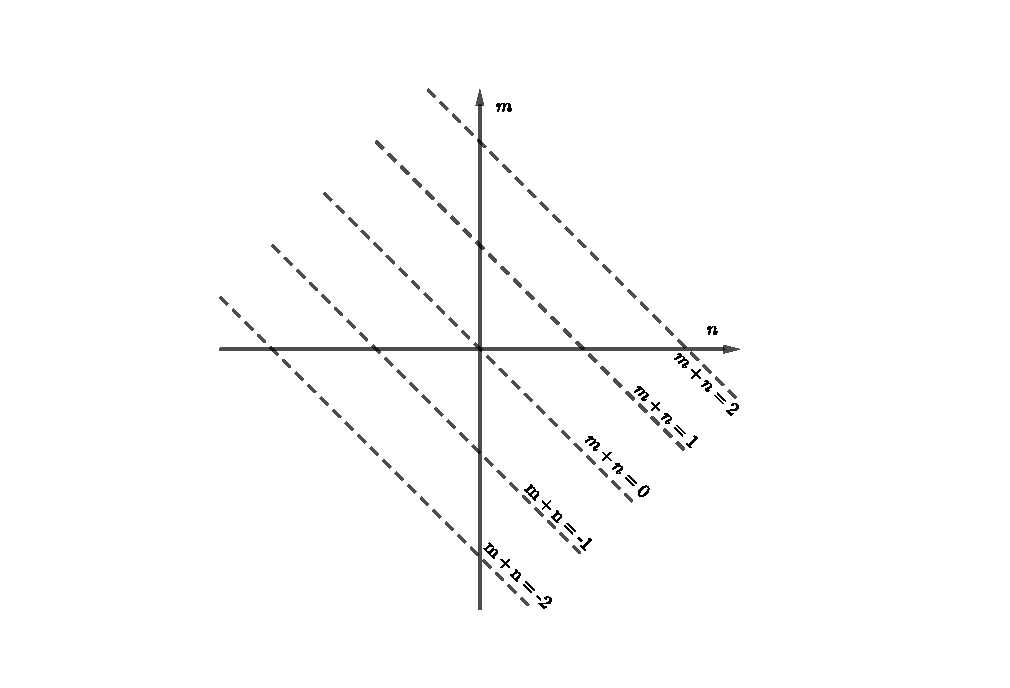
\includegraphics[width=\textwidth]{chapters/assets/rabi/summation-algebra}
    \caption{Rewrite multiplication of summations into summations only. The horizontal axis is for the summation index $n$ and the vertical axis is for the summation index $m$. The dashed lines are the lines of equal $m+n$.}
    \label{chap:matter-sec:jacobi-subsec:multi-matter-freq-fig:summation-algebra}
\end{figure}
The multiplication in Eqn.~\ref{chap:matter-sec:jacobi-subsec:multi-matter-freq-eqn:rabi-hamil-off} becomes
\begin{align}
   h =& \frac{\sin 2\theta_\mm}{2} \sum_{a = 1}^2 A_a \sin (k_a x + \phi_a) e^{-i\omega_\mm x} \nonumber\\
   &\sum_{N=-\infty}^{\infty} \sum_{n=-\infty}^{N} (-i)^n J_n (z_{k_1}) e^{i n(k_1 x + \phi_1) } (-i)^{N-n} J_{N-n}(z_{k_2}) e^{i (N-n)(k_2 x + \phi_2)} \nonumber\\
   =&\frac{\sin 2\theta_\mm}{2} \sum_{a = 1}^2 A_a \sin (k_a x + \phi_a) e^{-i\omega_\mm x} \nonumber\\
   &\sum_{N=-\infty}^{\infty} \sum_{n=-\infty}^{N} (-i)^N J_{n}(z_{k_1}) J_{N-n}(z_{k_2}) e^{i n ((k_1-k_2)x + \phi_1 - \phi_2) + i N (k_2 x + \phi_2)}
   \label{chap:matter-sec:jacobi-subsec:multi-matter-freq-eqn:stimulated-multi-freq-hamiltonian-12-element}
\end{align}
To proceed on, we rewrite $\sum_{a = 1}^2 A_a \sin (k_a x + \phi_a)$,
\begin{align}
   &A_1 \sin(k_1 x +\phi_1) + A_2 \sin(k_2 x +\phi_2) \nonumber\\
   = & \frac{A_1}{2i}\left( e^{i(k_1 x + \phi_1)} +  e^{-i(k_1 x + \phi_1)} \right) + \frac{A_2}{2i} \left( e^{i(k_2 x + \phi_2)} +  e^{-i(k_2 x + \phi_2)} \right).
\end{align}
We define
\begin{equation}
   h = h_1 + h_2,
\end{equation}
where
\begin{align}
   h_1 =& \frac{A_1\sin 2\theta_\mm}{4i}\bigg( \sum_{N=-\infty}^\infty \sum_{n=-\infty}^N (-i)^N J_n(z_{k_1}) J_{N-n}(z_{k_2}) e^{ i  \left(  (n+1) (k_1 x + \phi_1) +  (N-n)(k_2 x + \phi_2) - \omega_\mm x \right) } \nonumber \\
   & \sum_{N=-\infty}^\infty \sum_{n=-\infty}^N (-i)^N J_n(z_{k_1}) J_{N-n}(z_{k_2}) e^{ i \left(  (n-1) (k_1 x + \phi_1) + (N-n)(k_2 x + \phi_2) -  \omega_\mm x \right) }  \bigg),
\end{align}
and
\begin{align}
   h_2=& \frac{A_2\sin 2\theta_\mm}{4i}\bigg( \sum_{N=-\infty}^\infty \sum_{n=-\infty}^N (-i)^N J_n(z_{k_1}) J_{N-n}(z_{k_2}) e^{ i  \left(  n (k_1 x + \phi_1) + (N-n+1)(k_2 x + \phi_2) -  \omega_\mm x \right) } \nonumber\\
   & \sum_{N=-\infty}^\infty \sum_{n=-\infty}^N (-i)^N J_n(z_{k_1}) J_{N-n}(z_{k_2}) e^{ i  \left(  n (k_1 x + \phi_1) + (N-n-1)(k_2 x + \phi_2) -  \omega_\mm x \right) }  \bigg).
\end{align}
We keep only terms that are integers for each summation to satisfy the relations
\begin{align}
   (n_{11,N} + 1)k_1 + (N-n_{11,N}) k_2 -\omega_\mm &\sim 0 \\
   (n_{12,N} - 1)k_1 + (N-n_{12,N}) k_2 -\omega_\mm &\sim 0 \\
   n_{21,N}k_1 + (N-n_{21,N}+1) k_2 -\omega_\mm &\sim 0 \\
   n_{22,N} k_1 + (N-n_{22,N}-1) k_2 -\omega_\mm &\sim 0.
\end{align}
so that the $x$ dependent exponential almost vanishes (obtain the largest wavelength in fact). Notice that each $n_{ij,N}$ depends on the summation index $N$.

We solve each $n_{ij,N}$,
\begin{align}
   n_{11,N} &\sim \mathrm{Round}\left[\frac{\omega_\mm - N k_2 -k_1}{k_1 - k_2} \right] \\
   n_{12,N} &\sim \mathrm{Round}\left[\frac{\omega_\mm - N k_2 + k_1}{k_1 - k_2}\right] \\
   n_{21,N} &\sim \mathrm{Round}\left[\frac{\omega_\mm - (N + 1) k_2 }{k_1 - k_2} \right]\\
   n_{22,N} &\sim \mathrm{Round}\left[\frac{\omega_\mm - (N - 1) k_2 }{k_1 - k_2} \right].
\end{align}
Another important constrain is that $n\leq N$, thus we have
\begin{align}
   N_{11} &\sim \mathrm{Round}\left[\frac{\omega_\mm - k_1}{k_1}\right] \\
   N_{12} &\sim \mathrm{Round}\left[\frac{\omega_\mm + k_1}{k_1}\right] \\
   N_{21} &\sim \mathrm{Round}\left[\frac{\omega_\mm - k_2}{k_1}\right] \\
   N_{22} &\sim \mathrm{Round}\left[\frac{\omega_\mm + k_2}{k_1}\right],
\end{align}
for each summation over $N$ and we require $N\geq N_{ij}$ for each summation. We also assumed $k_1 > k_2$. In other words, $N_{ij}$ are the lower limits of the summations over $N$'s.

We keep only the resonance terms for the summation over $n$'s,
\begin{align}
   h_1 \approx & \frac{A_1\sin 2\theta_\mm}{4i} \bigg( \sum_{N=N_{11}}^\infty (-i)^N J_{n_{11}} (z_{k_1}) J_{N-n_{11}}(z_{k_2}) e^{ i \left(  (n_{11}+1) (k_1 x + \phi_1) + (N-n_{11})(k_2 x + \phi_2) - \omega_\mm x \right) }  \nonumber \\
   & \sum_{N=N_{12}}^\infty (-i)^N J_{n_{12}} (z_{k_1}) J_{N-n_{12}}(z_{k_2}) e^{ i \left(  (n_{12}-1) (k_1 x + \phi_1) + (N-n_{12})(k_2 x + \phi_2) - \omega_\mm x \right) }\bigg),
\end{align}
and
\begin{align}
   h_2 \approx & \frac{A_2\sin 2\theta_\mm}{4i} \bigg( \sum_{N=N_{21}}^\infty (-i)^N J_{n_{21}} (z_{k_1}) J_{N-n_{21}}(z_{k_2}) e^{ i \left(  n_{21} (k_1 x + \phi_1) + (N-n_{21} + 1)(k_2 x + \phi_2) - \omega_\mm x \right) }  \nonumber \\
   & \sum_{N=N_{22}}^\infty (-i)^N J_{n_{22}} (z_{k_1}) J_{N-n_{22}}(z_{k_2}) e^{ i \left(  n_{22} (k_1 x + \phi_1) + (N-n_{22}-1)(k_2 x + \phi_2) - \omega_\mm x \right) }\bigg) .
\end{align}

One can imagine how hard it is to solve the equation of motion with this $h$. More approximations are required. We will use the approximations that Kelly Patton et al used~\cite{Patton2014}.

By looking at the Hamiltonian, we can identify terms like this
\begin{align}
   h_a =& \left( \frac{\sin 2\theta_\mm}{2}  A_a \sin (k_a x + \phi_a) e^{-i\omega_\mm x}  \sum_{n=-\infty}^{\infty} (-i)^n J_n (z_{k_a}) e^{i n(k_a x + \phi_a) }  \right) \nonumber \\
   &\prod_{b\neq a} \sum_{n=-\infty}^{\infty} (-i)^n J_n (z_{k_b}) e^{i n(k_b x + \phi_b) },
\end{align}
where the parenthesis part is what we would have if only one frequency is used and we also have
\begin{equation}
   h = \sum_{a} h_a,
\end{equation}
for all frequencies.
This reminds us that each of these terms means the interference due to other frequencies. As a simple example, we demonstrate two-frequency case.

The two-frequency matter perturbation system has a Hamiltonian element $H_{12}$
\begin{equation}
   h = h_1 + h_2,
\end{equation}
where
\begin{align}
   h_1  =& {\color{blue}-\frac{k_1 \tan 2\theta_\mm}{2} \sum_{n_1=-\infty}^{\infty} (-i)^{n_1} n_1 J_{n_1} (z_{k_1}) e^{i (n_1 k_1-\omega_\mm)x} e^{i n_1\phi_1} }  \nonumber\\
   &{\color{red}\sum_{n_2=-\infty}^{\infty} (-i)^{n_2} J_{n_2}(z_{k_2}) e^{i(n_2k_2)x} e^{i n_2 \phi_2}  }, \\
   h_2 =& {\color{red} - \frac{k_2\tan 2\theta_\mm}{2} \sum_{n_2=-\infty}^{\infty} (-i)^{n_2} n_2 J_{n_2}(z_{k_2}) e^{i(n_2k_2-\omega_\mm)x} e^{i n_2 \phi_2}  } \nonumber\\
   &{\color{blue} \sum_{n_1=-\infty}^{\infty} (-i)^{n_1} J_{n_1}(z_{k_1}) e^{in_1 k_1 x} e^{i n_1 \phi_1} }
\end{align}
with red color coding the second frequency and blue coding the first frequency. $h$ is symmetric under exchange of index 1, 2 since the exchange simply switches $h_1$ and $h_2$.


The next question to ask is which term dominates. To grasp a clue, we need to identify which term in the summation dominates. Without a good analytical analysis, the only way to do is to numerically calculate the effect of each order.

By order, we are already thinking of a dominating term which is not true. Nonetheless, we assume RWA can be applied to the part that looks like one frequency only. In our two-frequency example, first RWA leads to
\begin{align}
   h_1  \approx & {\color{blue}-\frac{k_1 \tan 2\theta_\mm}{2} (-i)^{n_{1,0}} n_{1,0} J_{n_{1,0}} (z_{k_1}) e^{i (n_{1,0} k_1-\omega_\mm)x} e^{i n_{1,0}\phi_1} } \nonumber \\
   &{\color{red} \sum_{n_2=-\infty}^{\infty} (-i)^{n_2} J_{n_2}(z_{k_2}) e^{i(n_2k_2)x} e^{i n_2 \phi_2}  }, \\
   h_2  \approx & {\color{red} - \frac{k_2\tan 2\theta_\mm}{2} (-i)^{n_{2,0}} n_{2,0} J_{n_{2,0}}(z_{k_2}) e^{i(n_{2,0}k_2-\omega_\mm)x} e^{i n_{2,0} \phi_2}  } \nonumber \\
   &{\color{blue} \sum_{n_1=-\infty}^{\infty} (-i)^{n_1} J_{n_1}(z_{k_1}) e^{in_1 k_1 x} e^{i n_1 \phi_1} },
   \label{chap:matter-sec:jacobi-subsec:multi-matter-freq-eqn:eqn-after-first-rwa}
\end{align}
where
\begin{align}
   n_{1,0} &= \mathrm{Round}\left[  \frac{\omega_\mm}{k_1}  \right], \\
   n_{2,0} &= \mathrm{Round}\left[  \frac{\omega_\mm}{k_2}  \right] .
\end{align}
With this approximation, we can use RWA again by requiring
\begin{align}
   (n_{1,0} k_1-\omega_\mm + n_2 k_2)x &\sim 0, \\
   (n_1 k_1-\omega_\mm + n_{2,0} k_2)x &\sim 0,
\end{align}
where the integer solutions are
\begin{align}
   n'_{2,0} &= \mathrm{Round}\left[ \frac{ n_{1,0} k_1-\omega_\mm }{k_2} \right], \\
   n'_{1,0} &= \mathrm{Round}\left[ \frac{ n_{2,0} k_1-\omega_\mm }{k_1} \right].
\end{align}
Now we can remove all the summations using another RWA approximation. However, whether it holds is up to investigation.

The final result is
\begin{align}
   h_1 \approx & {\color{blue}-\frac{k_1 \tan 2\theta_\mm}{2} (-i)^{n_{1,0}} n_{1,0} J_{n_{1,0}} (z_{k_1}) e^{i (n_{1,0} k_1-\omega_\mm)x} e^{i n_{1,0}\phi_1} } {\color{red} (-i)^{n'_{2,0}} J_{n'_{2,0}}(z_{k_2}) e^{i(n'_{2,0}k_2)x} e^{i n'_{2,0} \phi_2}  } \nonumber \\
   =& -\frac{k_1 \tan 2\theta_\mm}{2} (-i)^{ n_{1,0}+n'_{2,0} }   e^{i (n_{1,0}\phi_1 + n'_{2,0} \phi_2)} n_{1,0} \nonumber\\
   &J_{n_{1,0}} (z_{k_1})  J_{n'_{2,0}}(z_{k_2}) e^{i(n_{1,0} k_1-\omega_\mm + n'_{2,0}k_2)x}  \\
   \equiv & \frac{F_1}{2} e^{i(n_{1,0} k_1-\omega_\mm + n'_{2,0}k_2)x}  , \\
   h_2 \approx & {\color{red} - \frac{k_2\tan 2\theta_\mm}{2} (-i)^{n_{2,0}} n_{2,0} J_{n_{2,0}}(z_{k_2}) e^{i(n_{2,0}k_2-\omega_\mm)x} e^{i n_{2,0} \phi_2}  }{\color{blue} \sum_{n_1=-\infty}^{\infty} (-i)^{n_1} J_{n_1}(z_{k_1}) e^{in_1 k_1 x} e^{i n_1 \phi_1} } \nonumber \\
   =& - \frac{k_2\tan 2\theta_\mm}{2} (-i)^{n_{2,0}+ n'_{1,0} }   e^{i (n_{2,0} \phi_2 + n'_{1,0} \phi_1)}  n_{2,0} \nonumber\\
   &J_{n_{2,0}}(z_{k_2})  J_{n'_{1,0}}(z_{k_1})  e^{i(n_{2,0}k_2-\omega_\mm+ n'_{1,0} k_1)x} \\
   \equiv & \frac{F_2}{2} e^{i(n_{2,0}k_2-\omega_\mm+ n'_{1,0} k_1)x} .
\end{align}


Lowest order only works for very special cases where on of the wave vectors is very close to resonance. To fix this problem, we could add more higher orders, however, what does it mean to have higher orders needs a discussion.

We will develop a protocol to decide which order to include. The first thought of higher orders is to add more from the summation before the last RWA. However, it is highly suspicious that this is just like the one frequency case which has a very fast drop in the resonance width as we go to higher orders. This guess needs proof, numerically and analytically. When we mentioned higher orders, we actually mean higher orders in both $n_1$ and $n_2$. Notice that we can always write the 12 element of Hamiltonian as Eqn.~\ref{chap:matter-sec:jacobi-subsec:multi-matter-freq-eqn:2-freq-hamiltonian-12-element}, i.e.,
\begin{align}
  h =& h_1 + h_2 \\
   =& \sum_{n_1=-\infty}^\infty \sum_{n_2=-\infty}^{\infty} B_{n_1,n_2}(k_1,k_2) \Phi e^{i(n_1 k_1 + n_2 k_2 - \omega_\mm)x}  \nonumber \\
  &+  \sum_{n_1=-\infty}^\infty \sum_{n_2=-\infty}^{\infty} B_{n_2,n_1}(k_2,k_1) \Phi e^{i(n_1 k_1 + n_2 k_2 - \omega_\mm)x} \nonumber\\
  =& \sum_{n_1=-\infty}^\infty \sum_{n_2=-\infty}^{\infty} \left( B_{n_1,n_2}(k_1,k_2) + B_{n_2,n_1}(k_2,k_1) \right) \Phi e^{i(n_1 k_1 + n_2 k_2 - \omega_\mm)x},
\end{align}
without any approximations.
\begin{itemize}
    \item One of the choices of adding higher orders is to use $n_1=\mathrm{Round}\left[ \frac{\omega_\mm}{k_1} \right]$ and $n_2=\mathrm{Round}\left[ \frac{ n_1  k_1 - \omega_\mm }{k_2} \right]$ as the lowest order in $h_1$ and $n_2=\mathrm{Round}\left[ \frac{\omega_\mm}{k_2} \right]$ and $n_1=\mathrm{Round}\left[ \frac{ n_2  k_2 - \omega_\mm }{k_1} \right]$ as the lowest order in $h_2$. Adding higher orders means we add or remove one from $n_1$ in $h_1$ and recalculate $n_2$, while add or remove one from $n_2$ in $h_2$ and recalculate $n_1$.

   That is to say, we always keep the RWA condition for the last RWA process. What can be changed is the first assumption that the most important term is when only one frequency is relevant which is not always true.

   As an example, we now consider $n_{i,\pm 1}=n_{i,0}\pm 1$ and $n'_{i,\pm 1} =  \mathrm{Round}\left[ \frac{ n_{j,\pm 1} k_j - \omega_\mm }{k_i} \right]$ with $j\neq i$, thus we replace $n_{i,0}$ with $n_{i,\pm 1}$ to get higher order corrections, c.f.~Fig.~\ref{chap:matter-sec:jacobi-subsec:multi-matter-freq-fig:compApproxNum}.


\begin{figure}[!htbp]
    \centering
    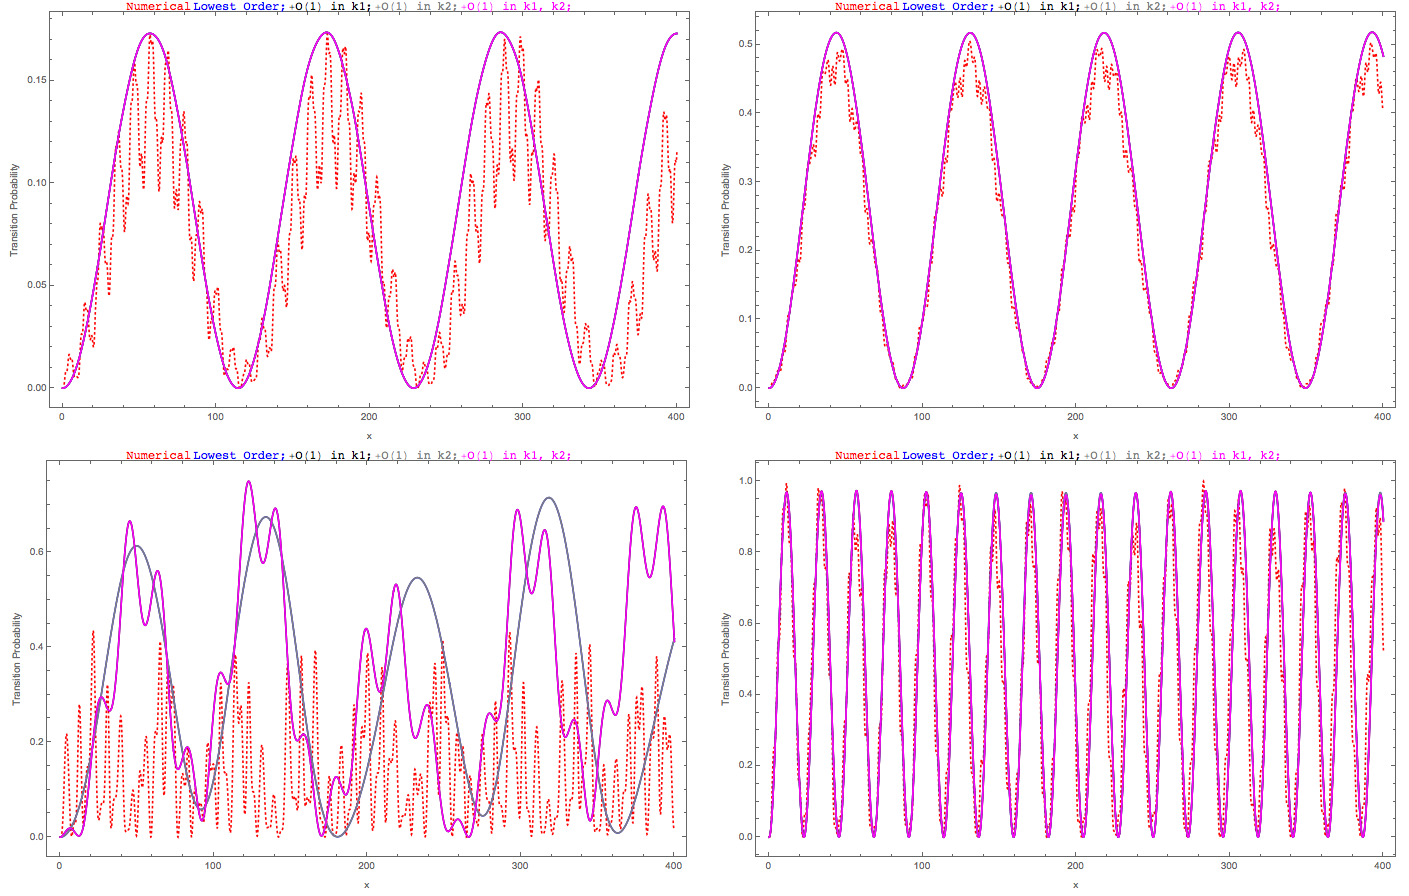
\includegraphics[width=\textwidth]{chapters/assets/rabi/compApproxNum.png}
    \caption{Top Left: Smaller wavenumber $k_1=0.95$ is at resonance and it has smaller perturbation amplitude ($k_2=1.55$);
      Top Right: Smaller wavenumber $k_1=0.95$ is at resonance and it has larger perturbation amplitude ($k_2=1.55$);
      Bottom Left: Larger wavenumber $k_2=0.95$ is at resonance and it has smaller perturbation amplitude ($k_1=0.35$);
      Bottom Right: Larger wavenumber $k_2=0.95$ is at resonance and it has larger perturbation amplitude ($k_1=0.35$).
      Red dotted line is numerical solution, black line is lowest approximation of $k_2$, magenta is higher order approximation of $k_2$.}
    \label{chap:matter-sec:jacobi-subsec:multi-matter-freq-fig:compApproxNum}
\end{figure}

   In realistic physical systems, it is more likely to have a matter profile so that we have the bottom left situation. In other words, RWA method breaks down in the most interesting case.

\item Another choice is to add or remove one for both $n_1$ and $n_2$ for both terms in the Hamiltonian. The approach will define the order $n_{order}$ first, as will be applied to the n's. As an example, adding first order to $n_1$ will include all the possible combinations of $n_1,n_1\pm 1$ for both terms without changing $n_2$. As an example, we compare the different orders of $n_1$ only with the numerical calculation without approximations in Fig.~\ref{chap:matter-sec:jacobi-subsec:multi-matter-freq-fig:stimulated-2-freq-higher-orders-approach-2}.


\begin{figure}[!htbp]
    \centering
    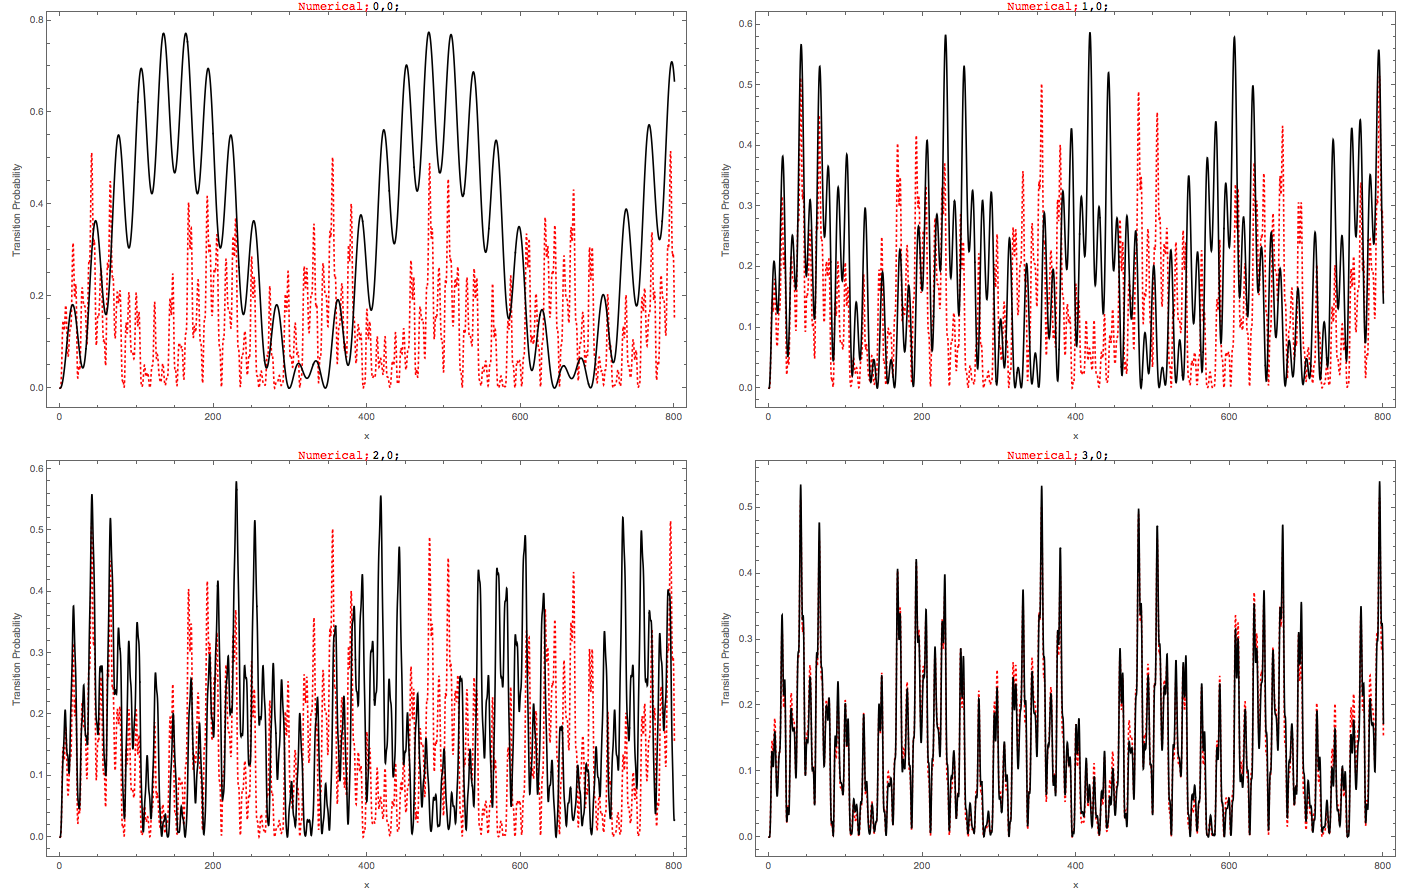
\includegraphics[width=\textwidth]{chapters/assets/rabi/stimulated-2-freq-higher-orders-approach-2.png}
    \caption{Compare the different orders with the numerical calculation without approximations, where red dotted line is the numerical calculation without approximation. As we could see from the figure, including up to third order in $n_1$ fixes the deviation from numerical calculation (red dotted line). The wave vectors are $k_1=0.5$, $k_2=0.8$, amplitudes are $A_1=0.1 k_1^{-5/3}$, $A_2=0.1 k_2^{-5/3}$, mixing angle in background matter is $\theta_\mm=\pi/5$.}
    \label{chap:matter-sec:jacobi-subsec:multi-matter-freq-fig:stimulated-2-freq-higher-orders-approach-2}
\end{figure}




\item Now according to the complete expression of the ${}_{12}$ element of Hamiltonian Eqn.~\ref{chap:matter-sec:jacobi-subsec:multi-matter-freq-eqn:2-freq-hamiltonian-12-element}, there is no difference between $n_1$ and $n_2$. Thus whenever we talk about different orders, we should not distinguish between the two integers. However, how to define zero order is not clear to me at this point. To find out, we need to know the resonance width of each pair of integers. The insight comes from the single frequency result. The width for single frequency $\Gamma = \left\lvert \frac{\hat F}{n_0} \right\rvert = \left\lvert \hat k \tan 2\theta_\mm \frac{ J_{n_0}( n_0 \hat A \cos 2\theta_\mm/\hat k )}{n_0} \right\rvert .
$ depends on the coefficient in front of the phase in the Hamiltonian and the integer. The task is to derive or guess the resonance width for each pair of integers $n_1, n_2$.

\end{itemize}


% .. admonition:: Which Approximation Breaks Down
%   :class: note

%   We ask the question, which approximation is breaking down exactly during our RWA? To find out, we first include all the orders after the first assumption, i.e., we do not use RWA for the second time, which means :eq:`eqn-after-first-rwa` holds but no RWA will be applied to this.

%   Not notice that the summation in :eq:`eqn-after-first-rwa` is due to the Jacobi-Anger expansion, which is not even helpful in our next calculation. Therefore, we trace back to their original expressions, which leads to

%   .. math::
%       h_1 & \approx {\color{blue}-\frac{k_1 \tan 2\theta_\mm}{2} (-i)^{n_{1,0}} n_{1,0} J_{n_{1,0}} (z_{k_1}) e^{i (n_{1,0} k_1-\omega_\mm)x} e^{i n_{1,0}\phi_1} } {\color{red} e^{-i z_{k_2} \cos(k_2 x+\phi_2)  } }, \\
%       h_2 & \approx {\color{red} - \frac{k_2\tan 2\theta_\mm}{2} (-i)^{n_{2,0}} n_{2,0} J_{n_{2,0}}(z_{k_2}) e^{i(n_{2,0}k_2-\omega_\mm)x} e^{i n_{2,0} \phi_2}  }{\color{blue}  e^{-i z_{k_1} \cos(k_1 x+\phi_1)  } }.

%   We then perform a numerical calculation using this Hamiltonian element and compare it with the full numerical results.



As for a more systematic treatment of the two-frequency case, we geometrize the problem. The 12 element can be written as
\begin{equation}
   h = h_1 + h_2,
\end{equation}
where
\begin{align}
   h_1 &=\sum_{n_1=-\infty}^\infty \sum_{n_2=-\infty}^{\infty}\left( -(-i)^{n_1+n_2}\frac{\tan 2\theta_\mm}{2} n_1 k_1 J_{n_1}(z_{k_1}) J_{n_2}(z_{k_2})  \right) e^{i(n_1\phi_1+n_2\phi_2)} e^{i(n_1 k_1 + n_2 k_2 - \omega_\mm)x}, \nonumber\\
   h_2 &=\sum_{n_1=-\infty}^\infty \sum_{n_2=-\infty}^{\infty}\left( -(-i)^{n_1+n_2}\frac{\tan 2\theta_\mm}{2} n_2 k_2 J_{n_1}(z_{k_1}) J_{n_2}(z_{k_2})  \right) e^{i(n_1\phi_1+n_2\phi_2)} e^{i(n_1 k_1 + n_2 k_2 - \omega_\mm)x}. \nonumber
\end{align}
For simplicity, we define
\begin{align}
   B_{n_1,n_2}(k_1,k_2,A_1,A_2) &= -(-i)^{n_1+n_2} \tan 2\theta_\mm n_1 k_1 J_{n_1}(z_{k_1}) J_{n_2}(z_{k_2}) \nonumber\\
   &= -(-i)^{n_1+n_2} \tan 2\theta_\mm n_1 k_1 J_{n_1}(\frac{A_1}{k_1}\cos 2\theta_\mm) J_{n_2}(\frac{A_2}{k_2}\cos 2\theta_\mm)  , \nonumber\\
   \Phi & = e^{i(n_1\phi_1+n_2\phi_2)}.\nonumber
\end{align}
Notice that
\begin{align}
   B_{n_2,n_1}(k_2,k_1, A_2, A_1) &= -(-i)^{n_1+n_2} \tan 2\theta_\mm n_2 k_2 J_{n_1}( \frac{A_1}{k_1}\cos 2\theta_\mm ) J_{n_2}( \frac{A_2}{k_2}\cos 2\theta_\mm ).\nonumber
\end{align}
Using these definitions, we rewrite the Hamiltonian 12 element
\begin{align}
   h =& h_1 + h_2 \\
    =& \frac{1}{2}\sum_{n_1=-\infty}^\infty \sum_{n_2=-\infty}^{\infty} B_{n_1,n_2}(k_1,k_2,A_1,A_2) \Phi e^{i(n_1 k_1 + n_2 k_2 - \omega_\mm)x} \nonumber\\
   &+  \frac{1}{2}\sum_{n_1=-\infty}^\infty \sum_{n_2=-\infty}^{\infty} B_{n_2,n_1}(k_2,k_1,A_2,A_1) \Phi e^{i(n_1 k_1 + n_2 k_2 - \omega_\mm)x}  \nonumber\\
    =& \frac{1}{2}\sum_{n_1=-\infty}^\infty \sum_{n_2=-\infty}^{\infty} \left( B_{n_1,n_2}(k_1,k_2,A_1,A_2) + B_{n_2,n_1}(k_2,k_1,A_2,A_1) \right) \Phi e^{i(n_1 k_1 + n_2 k_2 - \omega_\mm)x}  \nonumber\\
    =& \frac{1}{2}\sum_{n_1=-\infty}^\infty \sum_{n_2=-\infty}^{\infty} B_2{n_1,n_2}(k_1,k_2,A_1,A_2)\Phi e^{i(n_1 k_1 + n_2 k_2 - \omega_\mm)x},
   \label{chap:matter-sec:jacobi-subsec:multi-matter-freq-eqn:2-freq-hamiltonian-12-element}
\end{align}
where $B_2{n_1,n_2}(k_1,k_2,A_1,A_2)\equiv B_{n_1,n_2}(k_1,k_2,A_1,A_2) + B_{n_2,n_1}(k_2,k_1,A_2,A_1)$ is what we are interested in.

Comparing this expression with the single frequency one which is almost the same structure if we remove the two sums, and using the result \ref{chap:matter-sec:deep-jacobi-subsec:single-matter-freq-eqn:stimulated-single-freq-trans-probability}, we can infer that the transition probability,
\begin{equation}
    P_{1\to 2}(x) = \frac{\lvert \hat B_2 \rvert^2}{ \lvert \hat B_2 \rvert^2 + \hat g_2^2} \sin^2\left( \frac{q_2}{2}x \right),
\end{equation}
where $\hat B_2=\frac{ B_2 }{\omega_\mm}=\frac{B_{n_1,n_2}(k_1,k_2,A_1,A_2) + B_{n_2,n_1}(k_2,k_1,A_2,A_1)}{\omega_\mm}$ and $\hat g_2 = \frac{g}{\omega_\mm} = n_1 \hat k_1 + n_2 \hat k_2 - 1$ which tells us how far from resonance and $q_2=\sqrt{ \lvert \hat B_2 \rvert^2 + \hat g^2 }$.

The width then is similar to \ref{chap:matter-sec:deep-jacobi-eqn:single-frequency-width-guessing}, except that we could not define the width as a function of single variables since two wave vector are used. However, it is still reasonable to give the FWHM condition,
\begin{equation}
   n_1 \hat k_1 + n_2 \hat k_2 - 1 = \pm \lvert \hat B_2 \rvert = \left\lvert \frac{B_{n_1,n_2}(k_1,k_2,A_1,A_2) + B_{n_2,n_1}(k_2,k_1,A_2,A_1)}{\omega_\mm} \right\rvert.
   \label{chap:matter-sec:deep-jacobi-eqn:stimulated-2-freq-width-requirement-raw}
\end{equation}
For a given pair of integers $n_1,n_2$, we could find the amplitude as a function of $k_1, k_2$.

A solution shows that this is correct. The solution to the second element of wave function is
\begin{equation}
  \psi_{b2} = i \frac{ \lvert \hat B_2\rvert^2 e^{-\frac{i}{2} \hat g_2 \hat x} }{ \hat B_2 \sqrt{\lvert \hat B_2\rvert^2 + \hat g^2} }\sin\left( \frac{\sqrt{ \lvert \hat B_2 \rvert^2 + \hat g^2 }}{2}x \right)  .
\end{equation}

It is very confusing when we write down the requirement for width \ref{chap:matter-sec:deep-jacobi-eqn:stimulated-2-freq-width-requirement-raw}, since we need to assume $\lvert \hat F_2 \rvert$ to be almost constant to arrive this result. What values of $\hat k_1,\hat k_2$ do we need to calculate $\lvert \hat F_2 \rvert$? The idea is to find the FWHM (Full Width Half Maximum) when a point is deviating from the line. To be specific, we find the line that is the resonance using $n_1 k_1 + n_2 k_2 = 1$, which is plotted as dashed red line in \ref{chap:matter-sec:deep-jacobi-fig:diagram-of-width-2-freq}. To characterize the distance, we need a line that is perpendicular to this red dashed resonance line, which also is passing through the values of $(k_10,k_2)=(k_{10},k_{20})$ which is given in the system. Under this scheme, the resonance width is define as the distance from the resonance line when the amplitude reduces to half on this blue dotted perpendicular line.


\begin{figure}[!htbp]
    \centering
    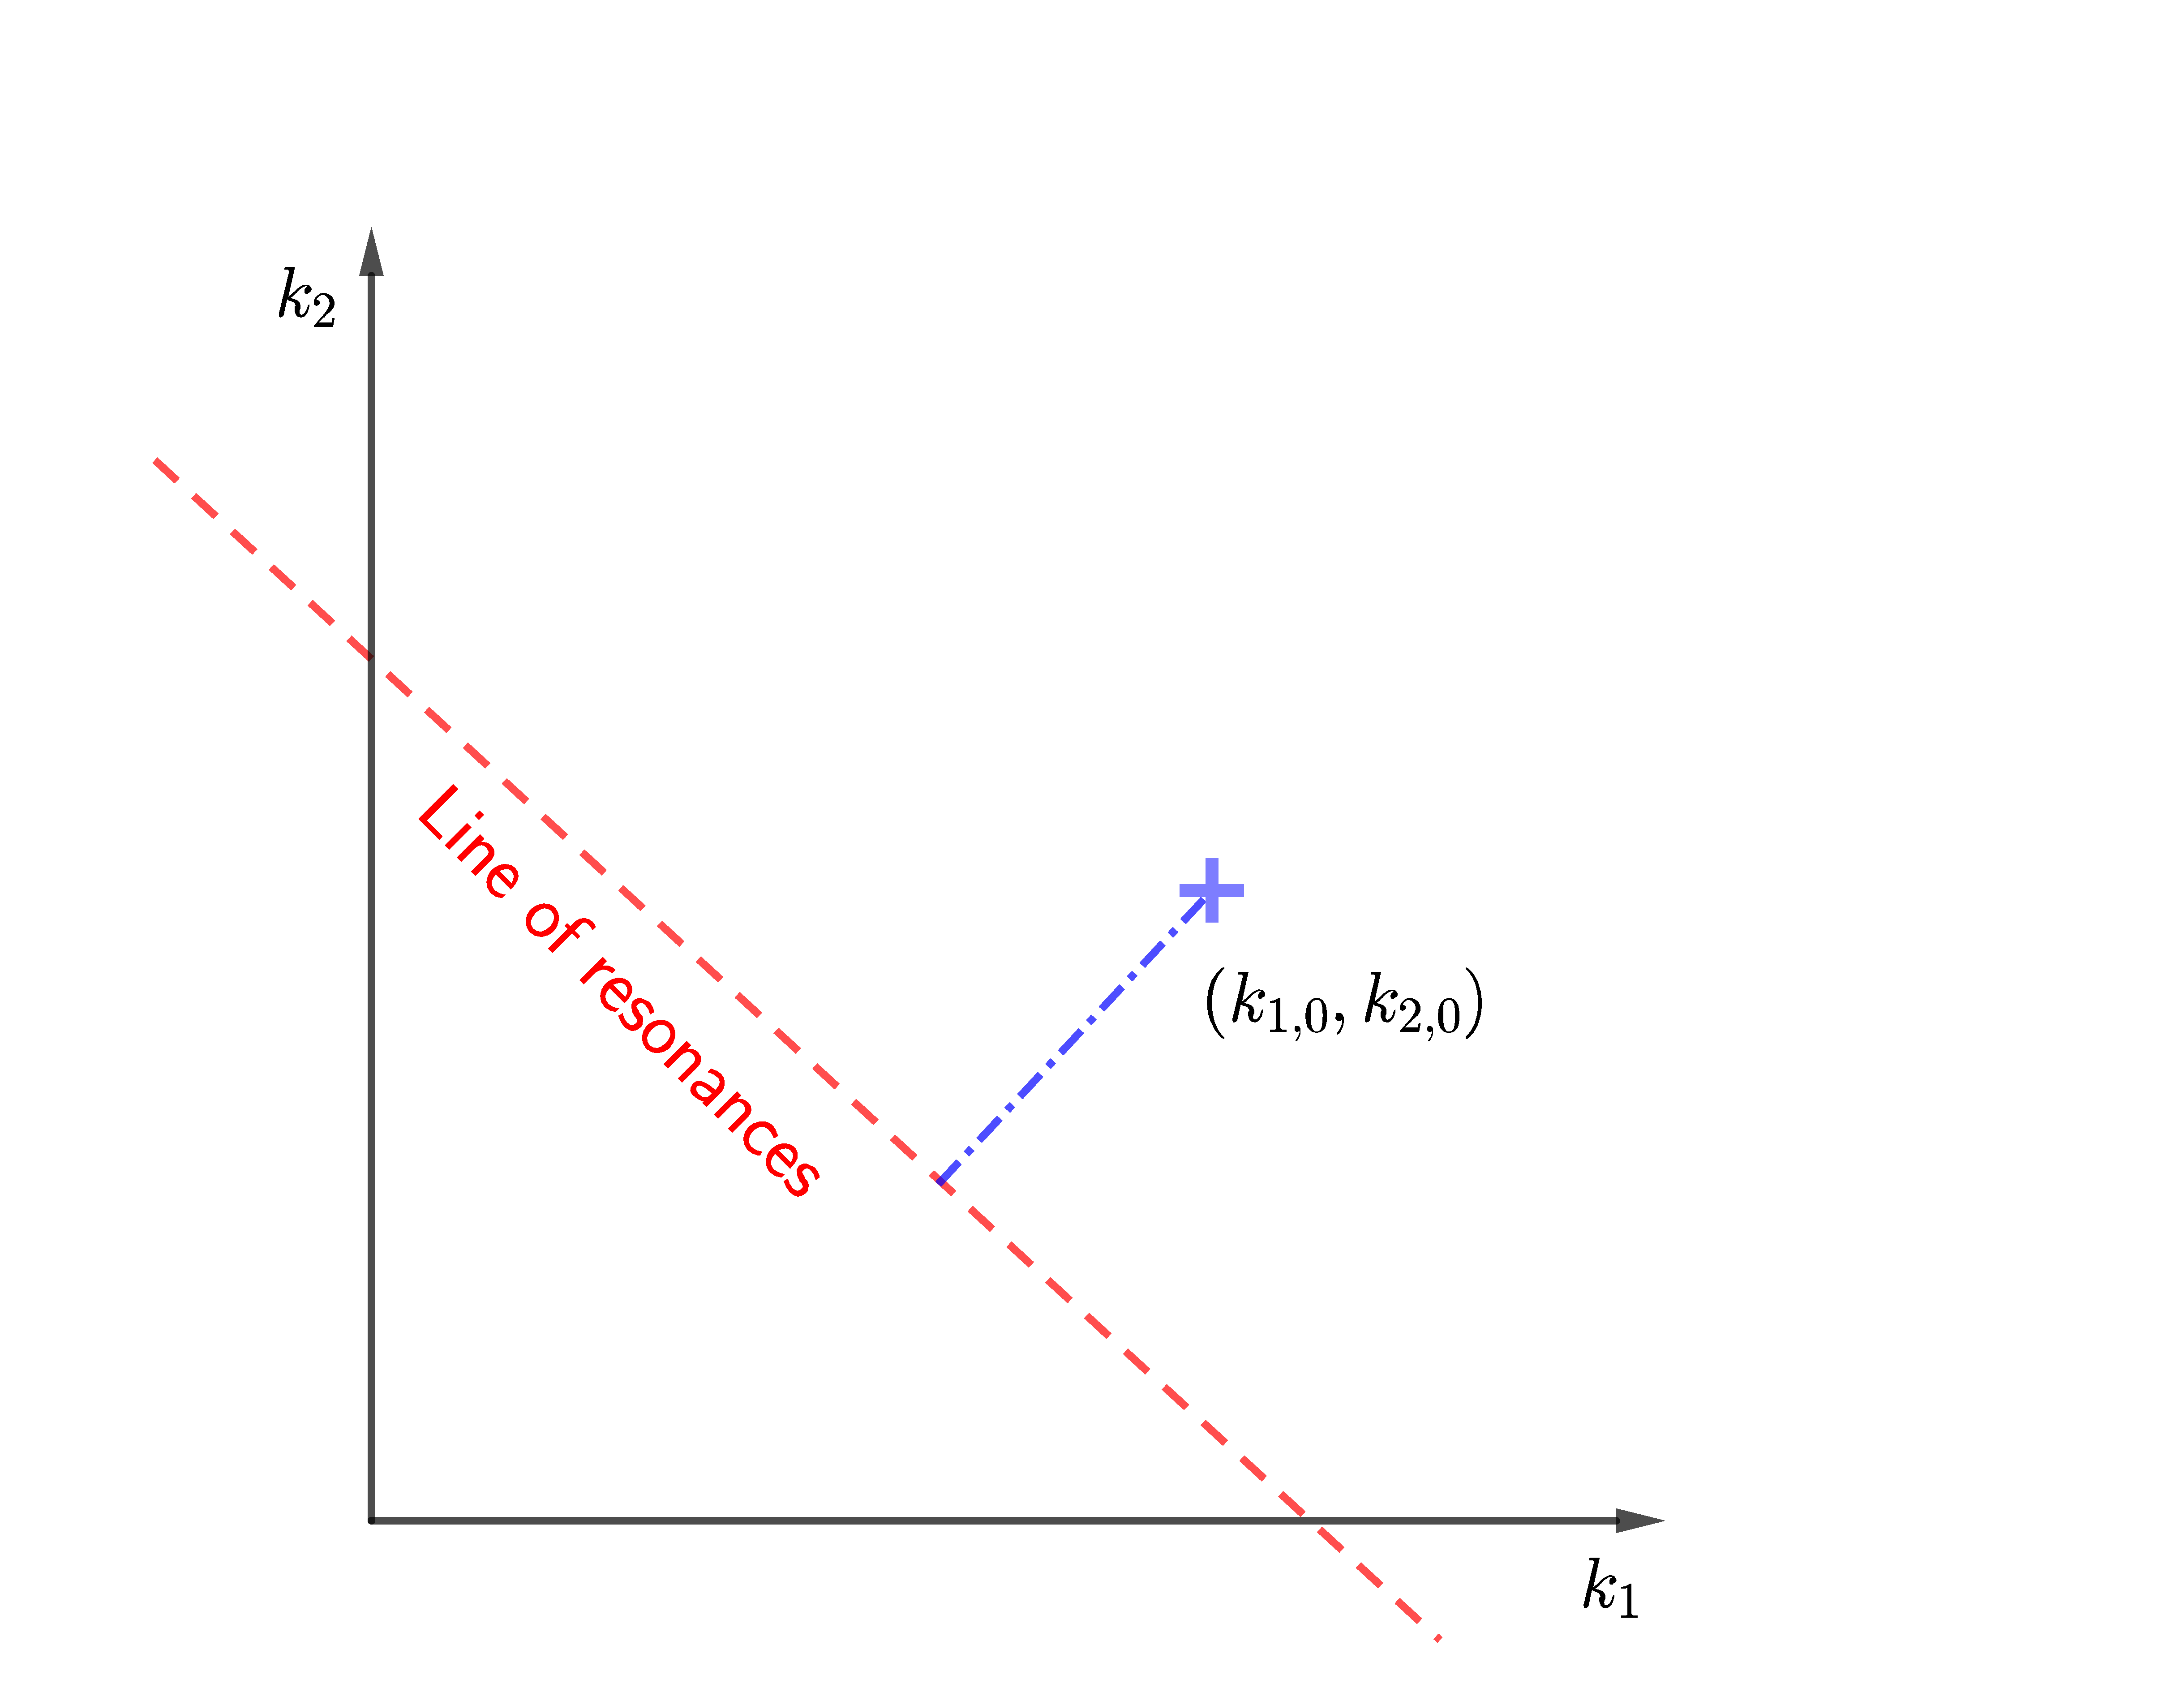
\includegraphics[width=\textwidth]{chapters/assets/rabi/stimulated-2-freq-width-diagram}
    \caption{Diagram of Width for two frequencies in matter density profile. The red dashed line is the line when the resonances happen. The cross is the location for a system that with two frequencies in density profile, $k_{1,0}$ and $k_{2,0}$. The blue dash dotted line indicates the distance between the actual frequencies of the system and the resonances. }
    \label{chap:matter-sec:deep-jacobi-fig:diagram-of-width-2-freq}
\end{figure}

In the language of algebra, we could derive the interception point of the two lines, which is
\begin{align}
   k_{1,\mathrm{intercept}} &= \frac{n_2^2 k_{10} + n_2 k_{20} + n_1 }{n_1^2 + n_2^2}, \\
   k_{2,\mathrm{intercept}} &= \frac{n_1}{n_2}k_{1,\mathrm{intercept}} - \frac{1}{n_2},
\end{align}
where $k_{10}$ and $k_{20}$ are the values given in the matter perturbation of the system.

Using this method, we can define a reasonable width for two frequency matter perturbation case,
\begin{equation}
   \Gamma_2 = \frac{B_2(k_{1,\mathrm{intercept}},k_{2,\mathrm{intercept}})}{\sqrt{n_1^2 + n_2^2}}.
\end{equation}

% .. admonition:: Derivation of Width for 2 Frequency Matter Perturbation
%   :class: hint

%   First of all, we assume that a point :math:`(\hat k_{10},\hat k_{20})` is a displace from the line by the FWHM :math:`\hat L` in :math:`\hat k_2`, which means that, the line that is paralell to the resonance line and passing through the point :math:`(\hat k_{10},\hat k_{20})` is displaced by :math:`\hat L` in :math:`\hat k_2`,

%   .. math::
%       n_1 \hat k_1 + n_2 \hat k_2 - n_2 \hat L = 1.

%   We assume the width of resonance is not large so that we could use resonance values for :math:`\hat k_1, \hat k_2`. For FWHM, we require

%   .. math::
%       n_1 k_{1,\mathrm{intercept}} + n_2 k_{2,\mathrm{intercept}} -1  - n_2 \hat L = \lvert \hat B_2(k_{1,\mathrm{intercept}},k_{2,\mathrm{intercept}}) \rvert,

%   where we could apply :math:`n_1 k_{1,\mathrm{intercept}} + n_2 k_{2,\mathrm{intercept}} -1 = 0` because we assumed the width is narrow, thus

%   .. math::
%       - n_2 \hat L = \lvert \hat B_2(k_{1,\mathrm{intercept}},k_{2,\mathrm{intercept}}) \rvert.


%   However, :math:`L` is not the actually deviation from the interception point. We could calculate the actual deviation :math:`\Gamma_2` on the blue line in figure :numref:`diagram-of-width-2-freq`, which is given by

%   .. math::
%       \sqrt{n_1^2 + n_2^2} \Gamma_2 = n_2 L,

%   i.e., we find the resonance width

%   .. math::
%       \Gamma_2 =  \frac{B_2(k_{1,\mathrm{intercept}},k_{2,\mathrm{intercept}})}{\sqrt{n_1^2 + n_2^2}}.


To apply the width in a problem, we need to calculate the distance between the given point $(k_{10},k_{20})$ of the system to a certain resonance line which depends on $n_1,n_2,A_1,A_2,\theta_\mm$. This is as simple as point to line distance, which is calculated using
\begin{equation}
   d = \frac{\lvert n_1 k_{10} + n_2 k_{20} - 1 \rvert}{\sqrt{n_1^2 + n_2^2} }.
   \label{stimulated-2-freq-distance-0}
\end{equation}
The requirement for a pair of $(n_1,n_2)$ to be important is determined by defining a quantity that compares the distance from a certain resonance line with the width of this resonance line,
\begin{equation}
   Q_2 = \frac{d}{\Gamma_2}.
\end{equation}




% .. admonition:: Caveats
%   :class: note

%   There are caveats when calculating the distance :math:`d` or the width :math:`\Gamma_2`.

%   The first problem is the zeros. In special cases, :math:`n_1=0` as an example, the distance :math:`d` using the equation :eq:`stimulated-2-freq-distance-0` will lead to infinities. Same thing happens to the width.

%   The solution is to treat the special cases seperately. As an result, we conclude that

%   .. math::
%       d=\begin{cases}
%       \frac{\lvert n_1 k_{10} + n_2 k_{20} -1 \rvert}{\sqrt{ n_1^2 + n_2 ^2 }}, & n_1\neq 0 \&\& n_2 \neq 0 \\
%       \infty , & & n_1= 0 \&\& n_2 = 0.
%       \end{cases}
%       :label: stimulated-2-freq-distance-d

%   The :math:`\infty` is simply a defined value which is to ensure the final values of :math:`Q_2` to be reasonable.

%   Meanwhile, the width can always be written as :math:`\Gamma_2 = \frac{B_2(k_{1,\mathrm{intercept}},k_{2,\mathrm{intercept}})}{\sqrt{n_1^2 + n_2^2}}.` as long as :math:`n_1\neq 0\&\& n_2\neq 0`. However, what we mean by :math:`k_{1,\mathrm{intercept}},k_{2,\mathrm{intercept}}` has special situations.

%   For :math:`n_1\neq 0\&\& n_2\neq 0`, we have the general solution

%   .. math::
%       k_{1,\mathrm{intercept}} &= \frac{n_2^2 k_{10} + n_2 k_{20} + n_1 }{n_1^2 + n_2^2}, \\
%       k_{2,\mathrm{intercept}} &= \frac{n_1}{n_2}k_{1,\mathrm{intercept}} - \frac{1}{n_2}.

%   For :math:`n_1=0\&\& n_2\neq 0`, we have

%   .. math::
%       k_{1,\mathrm{intercept}} &= k_{10}, \\
%       k_{2,\mathrm{intercept}} &= \frac{1}{n_2}.

%   Finally, for :math:`n_1\neq 0\&\& n_2 =0`, we need

%   .. math::
%       k_{1,\mathrm{intercept}} &=\frac{1}{n_1}, \\
%       k_{2,\mathrm{intercept}} &= k_{20}.

%   As for :math:`n_1=0\&\& n_2=0`, we define the width to be zero.

%   One last thing,

%   .. math::
%       Q_2 = \begin{cases}
%       \frac{d}{\Gamma_2}, & \Gamma_2\neq 0 \\
%       \infty, & \Gamma_2 = 0\&\& d\neq 0\\
%       0, & \Gamma_2=0\&\& d = 0
%       \end{cases}



\section{\label{conclusions}Conclusions}



The solar neutrinos behave very differently from lab experiments since the Sun provides a high matter density lab which can not be built on the Earth. What's even more exotic, in a supernova explosion, $10^{58}$ neutrinos are released from the proto-neutron star, which is of radius $10\mathrm{km}$, in a few seconds. The huge number density of neutrinos and large density of matter both change the neutrino oscillations dramatically. The matter effect in supernova is also much more complicated than MSW for solar neutrinos since the rich distribution of matter density and high speed motion. In addition to matter effect, neutrino neutrino interaction will be very efficient because of the high neutrino number density.

Apart from the emission of neutrinos from nuclear reactions of electron capture and positron emission in the solar interior, supernova environment also gives rise to Bremsstrahlung pair neutrino production, electron-positron neutrino pair production, which brings all three flavors and also anti-neutrinos into the spectra. However, even the with the presence of intensive interaction between neutrinos and the leptons and hardrons, which thermalize the neutrinos in the supernova core, the neutrino spectrum escaping from the supernova core is not completely Fermi-Dirac distribution. Nonetheless, it is possible to parametrize it using nominal Fermi-Dirac distribution,\cite{ysuzuki2004}
\begin{equation}
f(E)\propto \frac{E^2}{1+\exp ( E/kT - \mu )}.
\end{equation}
Some numerical results show that there is a deviation from this Fermi-Dirac distribution~\cite{Totani1998,Keil2003}. Meanwhile, Keil Mathias and Georg Raffelt showed that it is good enough to approximate the neutrino spectrum from supernova in Monte Carlo simulations using the so called "alpha fit",
\begin{equation}
f(E)\propto E^\alpha \exp\left( -(\alpha+1)\frac{E}{\langle E\rangle} \right),
\end{equation}
where $\langle E\rangle$ is the average energy, or the first moment of energy. The values from Monte Carlo simulations falls into the range $\alpha = 2.5\sim 5$,
which clearly shows the spectra are pinched. It's a hint that the detection of deviation from nominal Fermi-Dirac distribution will show evidence of core-collapse information.


% \begin{figure}
% \centering
% 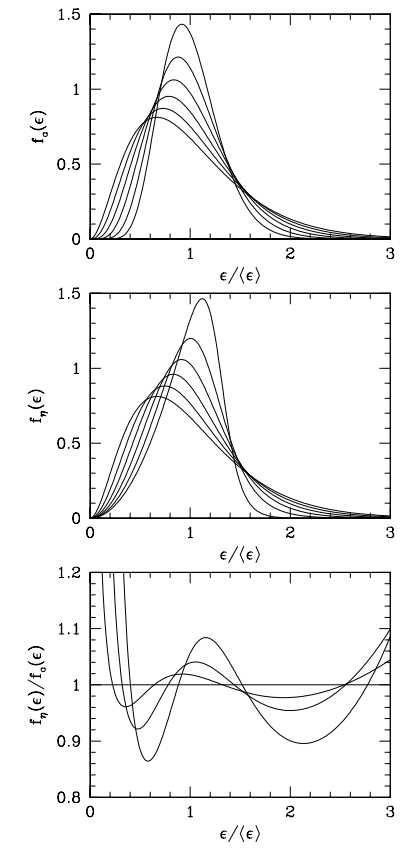
\includegraphics[width=\columnwidth]{chapters/assets/solar/neutrino_spectra_sn_simulations.png}
% \caption{Alpha fit and nominal Fermi-Dirac fit comparison. The top panel is alpha fit results while the middle panel is from nominal Fermi-Dirac distribution fit. The broadest curve are for $\alpha=2$. The width $w=\sqrt{\langle E^2 \rangle - \langle E\rangle^2}$ decrease 10\% for each curve. The bottom panel is the ratio of the two fit functions.}
% \label{fig:neutrino_spectra_sn_simulations}
% \end{figure}


Even though we understand solar neutrinos well, the neutrino oscillations of supernova explosions are not so to our complete knowledge. The flavor content is subject to the solution to the neutrino oscillations. Phenomena such as spectral split due to neutrino-neutrino interaction and matter effect reshape the neutrino spectra significantly. That being said, more research on supernova neutrinos, especially supernova neutrino oscillations is critical to understand supernova explosion mechanisms, as well as future observation of supernova neutrino data.


In conclusion, we have provided an interpretation for neutrino flavor conversion in fluctuating matter with the help of Rabi oscillations. The work provided two different points of view that is related to Rabi oscillations.

The first point of view was to interpret the neutrino flavor conversions in background matter basis. In this basis, matter density fluctuations will introduced a fluctuation part to the diagonal elements of the Hamiltonian, which means that the energy gap is fluctuating if we draw analogy between this Hamiltonian and the Hamiltonian of Rabi oscillations. For neutrino flavor conversions in a single frequency matter profile, the neutrino flavor oscillations becomes large when the matter fluctuation frequency is close to the energy gap, which is the resonance condition. We anticipated that the fluctuations of energy gap have limited effects on neutrino flavor conversions under this resonance condition. Thus the matter fluctuation only works as a pure flipping field that converts neutrinos from one flavor to another.

As we added more frequencies of matter density fluctuations, the neutrino flavor conversions becomes nontrivial due to the interferences between the difference matter profile frequencies. To quantify the interference between different Rabi oscillation modes, we defined relative detuning which describes how off-resonance a Rabi oscillation is. In the case of single frequency Rabi oscillations, the relative detuning becomes $0$ under the resonance condition. As a second frequency is added to the oscillations, the energy gap is shifted due to this new frequency. A measure of the interference effect is to consider the relative detuning of the first frequency which is at resonance, under the shifted energy gap. Numerical results verified this conjecture. With the interference mechanism, we revisit the single frequency matter profile neutrino oscillations.

Another view is to switch to a basis where the neutrino oscillations Hamiltonian is decomposed into infinite Rabi oscillations. Equivalently speaking, the oscillations are consequences of superposition of Rabi oscillations, which we call modes of oscillations. This view was applied to emphasis the approximations that the change of energy gap due to matter fluctuation can be neglected under resonance condition in the previous background matter basis.











% \section{\label{acknowledgement}Acknowledgement}

% The first author would like to thank J. Kneller and K. Patton for their help during this research. This research is supported by DOE EPSCoR grant \#DE-SC0008142.

%!TEX root = ../phd-thesis-lei-ma.tex

\chapter{\label{chap:collective}Collective Neutrino Oscillations}

Neutrino oscillations in the matter background have well defined linear dynamics as I  have discussed in the preceding chapters. In this chapter, I will discuss neutrino oscillations in a dense neutrino medium where the equation of motion becomes nonlinear. 
%However, the universe provides many other much more exciting labs for neutrino physics. 
One of such examples is the (core-collapse) supernova explosion which releases approximately $10^{58}$ neutrinos within seconds~\cite{Bahcall1987}. The neutrino density inside a supernova can be so large that that the neutrino self-interaction potential $H_{\nu\nu}$ to be comparable to or even larger than the matter potential in certain regions~\cite{Flowers1976a}. It has been shown that the self-interaction between the neutrinos can cause the neutrino medium to oscillate collectively~\cite{Duan2010, Duan2006}. The neutrino self-interaction also introduces a new characteristic energy scale which is proportional to the neutrino number density. As a result it is possible that neutrinos can oscillate on distance scales much shorter than the vacuum neutrino oscillation wavelength [cite ray sawyer, and raffelt].
%~\cite{Malkus2014, Vaananen2015, Wu2015}.

In this chapter, I will first review some of the general features of collective neutrino oscillations and introduce the method of linearized flavor stability analysis. I will then discuss the dispersion relation of the collective modes of neutrino oscillations and show that it may or may not be related to the flavor stability of neutrino gas. Finally, I will demonstrate an preliminary study of a toy model which can be used to understand the neutrino oscillations in the presence of the neutrino halo [cite neutrino halo paper].
% review the neutrino collective oscillations and fast modes in neutrino collective oscillations. I will also review the connection between fast modes and dispersion relations proposed by I. Izaguirre et al~\cite{Izaguirre2016a}. Then I will show that the relation dispersion relations and fast modes is not well established. In the last few sections, I will discuss the neutrino halo problem, where scattering of neutrinos is considered.


% \section{\label{chap:collective-sec:collective}Collective Oscillations}


% \section{\label{chap:collective-sec:synchronization}Synchronization in Neutrino Oscillations}
% \section{\label{chap:collective-sec:collective}Collective Oscillations}
\section{Equation of Motion}

The equation of motion for neutrino oscillations with self-interaction is\cite{Sigl1993}
\begin{equation}
   \ri \frac{d}{dt}\rho = [ \mathsf H,\rho],
   \label{chap:collective-sec:collective-eqn:equation-of-motion-general}
\end{equation}
where the total derivative is
\begin{equation}
   \frac{d}{dt} = \partial_t + \mathbf v\cdot \boldsymbol{\nabla},
\end{equation}
and the Hamiltonian Hamiltonian is composed of three different terms:
\begin{equation}
   \mathsf H = \mathsf H_{\mathrm v} + \mathsf H_{\mathrm m} +\mathsf  H_{\nu\nu}.
\end{equation}
% \begin{equation}
%     \frac{d}{dt} = \frac{d}{dr},
%  \end{equation}
%  where $r$ is the distance travelled by the neutrino. A more general approach is to rewrite the total derivative
In the above equation, the vacuum Hamiltonian is
%$\mathsf H_\vv$, $\mathsf H_\mm$ and $\mathsf H_{\nu\nu}$ represents the vacuum Hamiltonian, matter potential, and neutrino self-interaction potential:
\begin{align*}
    \mathsf H_\vv =& \begin{cases}
    -\frac{1}{2}\eta \omega_\vv \sigma_3 & \text{for neutrinos},\\
    \frac{1}{2}\eta \omega_\vv \sigma_3 & \text{for antineutrinos},
    \end{cases}
\end{align*}
and the matter potential is 
\begin{equation}
    \mathsf H_\mm = \frac{1}{2} \lambda \sigma_3  = \frac{1}{2} \sqrt{2}G_{\mathrm F} n_{\mathrm e} \sigma_3,
\end{equation}
where $\eta = +1$ for the normal neutrino mass hierarchy and $-1$ for the inverted neutrino mass hierarchy, $\omega_\vv$ is the vacuum oscillation frequency of the neutrino or antineutrino, and $n_{\mathrm e}$ is the net electron number density. The neutrino self-interaction is more complicated and can be written as
\begin{equation}
    \mathsf H_{\nu\nu} = \sqrt{2}G_{\mathrm F} \int dE' d\Omega_{\mathbf v'} \left[ n(E',\mathbf v')\rho(E',\mathbf v') - \bar n(E',\mathbf v')\bar\rho(E',\mathbf v') \right] (1-\mathbf v \cdot \mathbf v'),
    \label{chap:collective-sec:collective-eqn:equation-of-motion-self-interaction}
\end{equation}
where $n(E,\mathbf v)$ and $\rho(E, \mathbf v)$ are the number density and the flavor density matrix of the neutrino with energy $E$ and velocity $\mathbf v$, and $\bar n(E, \mathbf v)$ and $\bar \rho(E,\mathbf v)$ are the corresponding quantities of the antineutrino.
% \begin{align}
%     \mathsf H_\vv =& -\frac{1}{2}\beta\eta \omega_0 \sigma_3\\
%     \mathsf H_\mm =& \frac{1}{2} \sqrt{2}G_F n_e \sigma_3 \\
%     \mathsf H_{\nu\nu} =& \sqrt{2}G_F \int d\omega d\Omega_{\mathbf v'} n(\omega,\mathbf v')\beta(\mathbf v')\rho(\omega,\mathbf v') (1-\mathbf v \cdot \mathbf v').
% \end{align}
% I use $\eta=\pm 1$ for Normal Hierarchy and Inverted Hierarchy respectively. I also use $\beta=1$ for neutrinos and $\beta=-1$ for antineutrinos. In other words, the vacuum frequency is $\omega_\vv = \eta \omega_0$. $\beta(\mathbf v')$ indicates whether the density matrix $\rho(\omega,\mathbf v')$ is for neutrinos or antineutrinos. If $\beta(\mathbf v')=-1$, $\rho(\omega,\mathbf v')$ is for antineutrinos, vice versa. More explicitly, the vacuum Hamiltonian is
% \begin{align*}
%    \mathsf H_\vv =& \begin{cases}
%    -\frac{1}{2}\eta \omega_\vv \sigma_3 & \text{for neutrinos}\\
%    \frac{1}{2}\eta \omega_\vv \sigma_3 & \text{for antineutrinos}
%    \end{cases}
% \end{align*}
% while the neutrino-neutrino interaction Hamiltonian is
% \begin{align*}
%    \mathsf H_{\nu\nu} =& %\begin{cases}
%    \sqrt{2}G_{\mathrm F} \int d\omega d\Omega_{\mathbf v'} n(\omega,\mathbf v')\rho(\omega,\mathbf v') (1-\mathbf v \cdot \mathbf v') & \text{interacting with neutrinos} \\
%    - \sqrt{2}G_{\mathrm F} \int d\omega d\Omega_{\mathbf v'} n(\omega,\mathbf v')\bar\rho(\omega,\mathbf v') (1-\mathbf v \cdot \mathbf v') &  \text{interacting with antineutrinos}
% %    \end{cases}
% \end{align*}

% Please note that I have used the following notation.
% \begin{itemize}
%     \item $\omega_\vv$ is the absolute value of the frequency, since $\eta$ takes care of the signs;
%     \item The integral in $\mathsf H_{\nu\nu}$ must take care of both interactions with neutrinos and anti-neutrinos.
% \end{itemize}
% I also use the following quantities in this chapter.
% \begin{itemize}
%     \item $\lambda$ is the same as the previous chapter
%     \begin{equation}
%         \lambda = \sqrt{2} G_{\mathrm F} n_{\mathrm e}.
%     \end{equation}
% \item Angle distribution of number density is denoted as
% \begin{equation}
%     f(\mathbf v) = \frac{n(\omega,\mathbf v)}{n_{\mathrm{t}}},
% \end{equation}
%    where $n_{\mathrm{total}}$ is the total number density of neutrinos for all energies. It can also be defined for anti-neutrinos
% \begin{equation}
%       \bar f(\mathbf v) = \frac{\bar n(\omega,\mathbf v)}{\bar n_{\mathrm{t}}},
% \end{equation}
% where $\bar n_{\mathrm{t}}$ is the total number density of antineutrinos. One of the useful models is the line model, where neutrinos are emitted from a line. This model is a 2D neutrino problem. The direction of momentum $\mathbf v$ only depends on one angle, hence the distribution becomes $f(\theta)$. With this definition, the number density of neutrinos for some specific frequency $\omega$ within a range of angle $[\theta, \theta + d\theta]$ can be calculated using
% \begin{equation}
%       n_{\mathrm{t}} f(\theta) d\theta.
% \end{equation}
% Similarly, the the number density of antineutrinos within angle $[\theta,\theta+d\theta]$ is
% \begin{equation}
%     \bar n_{\mathrm{t}} \bar f(\theta) d\theta.
% \end{equation}
% \item An asymmetry parameter can be defined to connect the total number density of neutrinos and antineutrinos,
% \begin{equation}
%     \alpha = \frac{\bar n_{\mathrm{t}} }{n_{\mathrm{t}}}.
% \end{equation}

% \end{itemize}

% With the three definitions we simplify the neutrino self-interactions with matter effect
% \begin{align*}
%     \mathsf H_\mm =& \frac{1}{2} \lambda \sigma_3 \\
%     \mathsf H_{\nu\nu} =& \sqrt{2}G_{\mathrm F} n_{\mathrm{t}} \int d\omega d\Omega_{\mathbf v'} f(\omega,\mathbf v)\rho(\omega,\mathbf v') (1-\mathbf v \cdot \mathbf v') \\
%    & - \sqrt{2}G_{\mathrm F} \bar n_{\mathrm{t}} \int d\omega d\Omega_{\mathbf v'} \bar f(\omega,\mathbf v)\bar\rho(\omega,\mathbf v') (1-\mathbf v \cdot \mathbf v') \\
%    =& \frac{1}{2}\mu \int d\omega d\Omega_{\mathbf v'} f(\omega, \mathbf v)\rho(\omega,\mathbf v') (1-\mathbf v \cdot \mathbf v') \\
%    & - \frac{1}{2}\alpha \mu \int d\omega d\Omega_{\mathbf v'} \bar f(\omega, \mathbf v)\bar\rho(\omega,\mathbf v') (1-\mathbf v \cdot \mathbf v') ,
% \end{align*}
% where
% \begin{equation}
%    \mu = 2\sqrt{2} G_{\mathrm F} n_{\mathrm{t}}.
% \end{equation}

The presence of the neutrino self-interaction potential make the equation of motion \ref{chap:collective-sec:collective-eqn:equation-of-motion-general} nonlinear, and many interesting phenomenon arise because of it. For example, a dense neutrino medium can experience synchronized oscillation during which all the neutrinos and antineutrinos oscillate with the same frequency [cite raffelt paper]. To see this, I will consider an isotropic and homogeneous neutrino gas and use the flavor isospin picture discussed in Sec.~\ref{chap:basics-sec:flavor-isospin-pic}. The flavor isospin of the neutrino is defined by
% With the equation of motion Eqn.~\ref{chap:collective-sec:collective-eqn:equation-of-motion-general}, many aspects of such a system can be explored, such as neutrino bulb model, line model, etc. New dynamics, such as spectral split, synchronizations, matter-neutrino resonances, have been identified~\cite{Duan2006,Malkus2014,Vaananen2015}. Synchronization is one of the most surprising results which might happen when neutrino number density is large.
\begin{equation}
   \rho = \frac{1}{2} + \vec s \cdot \vec \sigma.
\end{equation}
% and that of the antineutrino is defined by
% \begin{equation}
%     \bar\rho = \frac{1}{2} - \vec s \cdot \vec \sigma.
% \end{equation}
% The reason for the negative sign in the above definition for the antineutrino is due to the sign in front of $\bar \rho(E, \mathbf v)$ in Eqn.~\ref{chap:collective-sec:collective-eqn:equation-of-motion-self-interaction}.
The equation of motion of the flavor isospin is
\begin{equation}
    \dot{\vec s} = \vec s \times \left(\vec H_\vv + \vec H_{\nu\nu} \right),
    \label{chap:collective-eqn:flavor-isospin-eom}
\end{equation}
where
\begin{equation}
   \vec H_{\mathrm v} =  \omega_{\mathrm v}\begin{pmatrix}
   -\sin 2\theta_{\mathrm v}\\
   0 \\
   \cos 2\theta_{\mathrm v}
   \end{pmatrix} = \omega_\vv \vec B,
\end{equation}
and
\begin{equation}
\vec H_{\nu\nu} = \sqrt{2}G_{\mathrm F} \int d E' n(E') \vec s(E').
\end{equation}
Here for simplicity I have assumed $n_{\mathrm e}=0$ and $\bar n=0$. When the neutrino density is very large, $\vec H_{\nu\nu}$ dominates over $\vec H_\vv$ in Eqn.~\ref{chap:collective-eqn:flavor-isospin-eom}, and $\vec s_\vv$ precesses about $\vec H_{\nu\nu}$ rapidly. Meanwhile, the total flavor isospin
\begin{equation}
    \vec S = \int d E' f(E') \vec s(E') 
\end{equation}
precesses about $\vec H_\vv$ slowly with a mean oscillation frequency $\langle omega_\vv \rangle$, where
\begin{equation}
    f(E) = \frac{ n(E) }{ \int dE' n(E') }
\end{equation}
is the energy distribution of the neutrino. To see this, one can multiply Eqn.~\ref{chap:collective-eqn:flavor-isospin-eom} by $f(E)$ and integrate over $E$ which gives
\begin{align}
    \dot{\vec S} &= \int dE f(E)\vec s(E) \times \omega_\vv \vec B \\
    &\to \int dE f(E) \left[ \frac{\vec s(E) \cdot \vec S}{ \lvert \vec S \rvert^2 } \vec S \right] \times \omega_\vv \vec B \\
    &= \langle \omega_\vv \rangle \vec S \times \vec B,
\end{align}
where
\begin{equation}
    \langle \omega_\vv \rangle  = \int dE f(E) \left[ \frac{\vec s(E) \cdot \vec S}{ \lvert \vec S \rvert^2 } \right] \omega_\vv.
\end{equation}
In the above equation I have replaced flavor isospin $\vec s$ with its projection along the direction of $\vec S$ because its precession about $\vec S$ is much faster than the precession of $\vec S$ about $\vec B$.

% But the neutrino coherent scattering term requires some simplifications. For the purpose of the physics picture, we consider isotropic and homogeneous model composed of neutrinos only which leads to
% \begin{equation}
%    \vec H_{\nu\nu} = \sqrt{2}G_{\mathrm F} n_\nu \int d\vec p'^3 (1-\vec p \cdot \vec p') (\rho_{\vec p'} - \bar\rho_{\vec p'}) = \sqrt{2}G_{\mathrm F} n_\nu \int dE' \frac{1}{n_\nu}(\rho_{E'} - \bar\rho_{E'}).
%    \label{chap:collective-sec:collective-eqn:isotropic-homogeneous-self-interaction}
% \end{equation}
% The flavor isospin will precess around $\vec H_{\nu\nu}$ assuming no vacuum or matter contributions.%, as shown in Fig.~\ref{chap:collective-sec:collective-fig:self-interaction}. 
% We have to define a vector, which is an integral of flavor-isospin vector over all energies or frequencies,
% \begin{equation}
%    \vec D = \int d\omega' \vec s(\omega').
% \end{equation}
% Eqn.~\ref{chap:collective-sec:collective-eqn:isotropic-homogeneous-self-interaction} becomes $\vec H_{\nu\nu} = \mu \vec D$, where $\mu = \sqrt{2}G_{\mathrm F} n_\nu$.

% \begin{figure}[h!tbp]
%     \centering
%     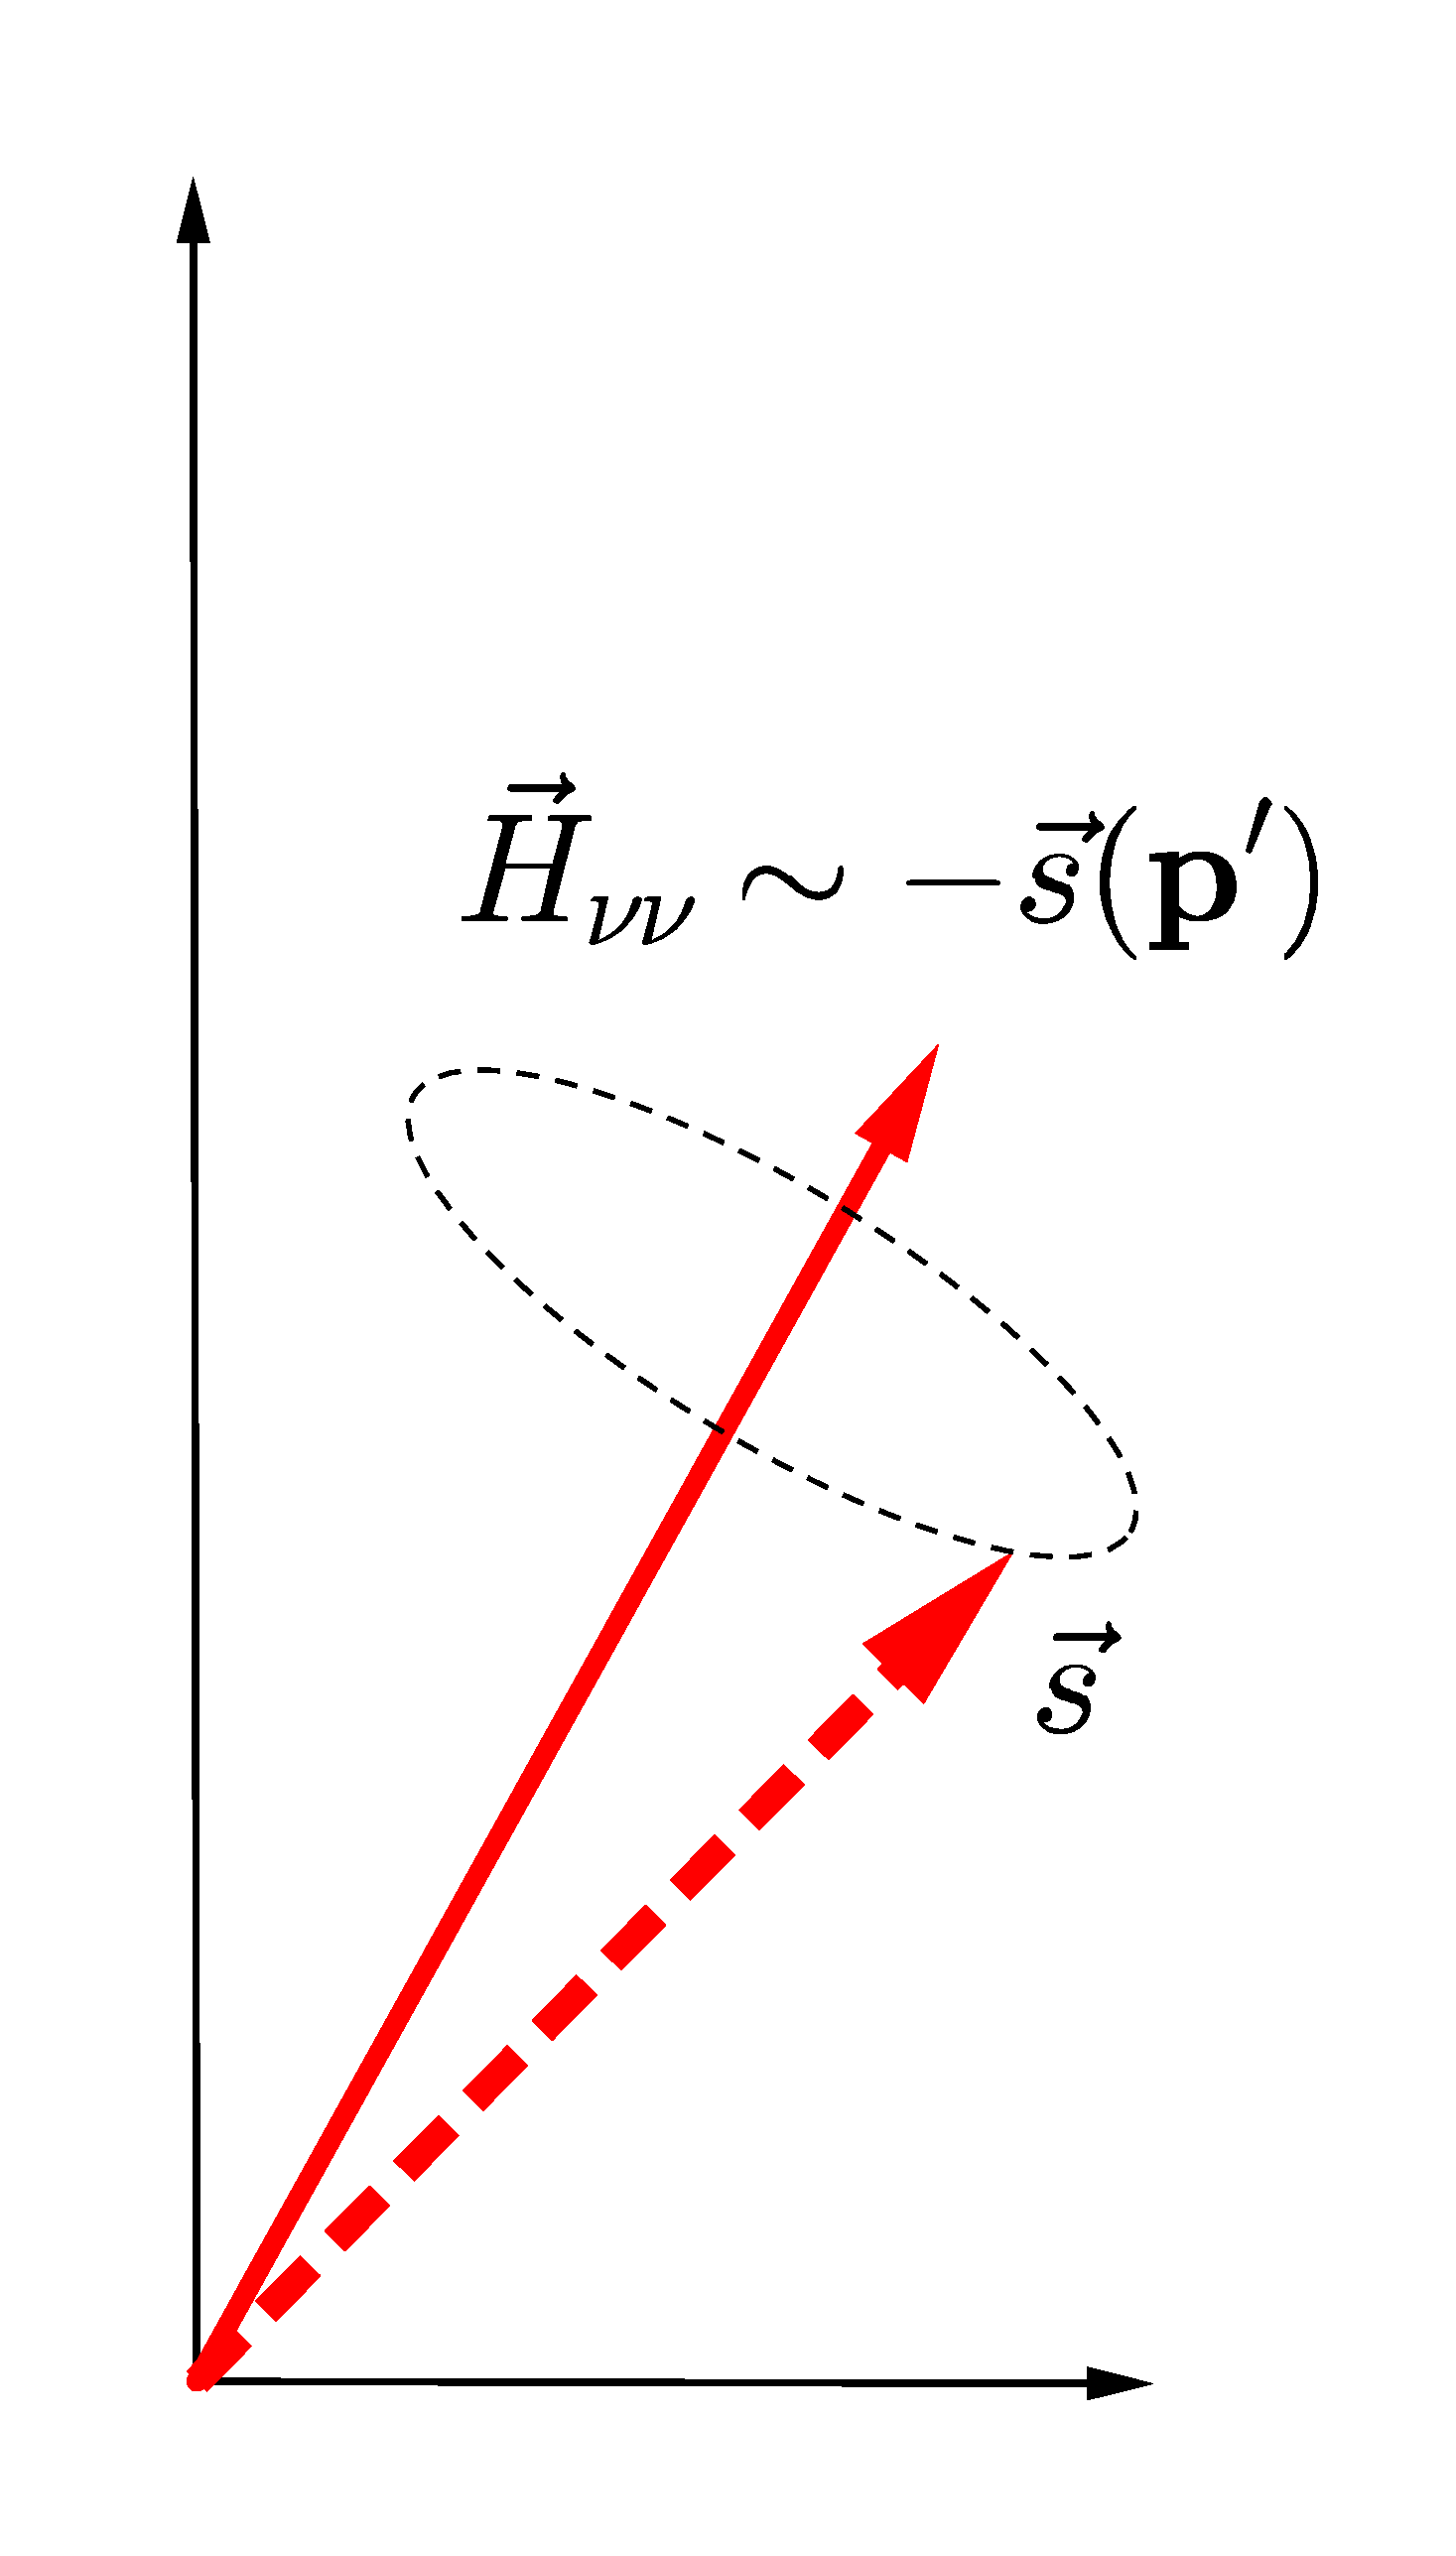
\includegraphics[width=0.4\textwidth]{chapters/assets/matter/self-interaction}
%     \caption{ Flavor isospin $\vec s$ precess around the Hamiltonian $\vec H_{\nu\nu}$ in flavor isospin space.}
%     \label{chap:collective-sec:collective-fig:self-interaction}
%  \end{figure}


% For single energy or flavor isospins aligned in the same direction, this vector is in the direction of the flavor isospin vector. If the flavor isospins are initially prepared in completely random and uniformly distributed directions, $\vec D\sim 0$.

% Synchronization occurs when the neutrino number density becomes large. $\vec D$ will wobble around very fast due to the precessions of flavor isospins, but almost stays in one direction. All the spins precess with the same frequency which is determined by $\mu$.

% With vacuum contribution $\vec H_{\mathrm v}$ and matter contribution $\vec H_{\mathrm m}$ to the Hamiltonian, we expect $\vec D$ to precess around $\vec H_{\mathrm v} + H_{\mathrm v}$, if the precession frequency of flavor isospins around $\vec D$ is much larger than the precession frequency of $\vec D$ around  $\vec H_{\mathrm v} + H_{\mathrm v}$.



\section{\label{chap:collective-sec:two-beams}Two Beams Model and Linear Stability Analysis}

Since neutrino oscillations with self-interactions is nonlinear, linear stability analysis comes into the play. I will go through the procedure and demonstrate the significance of instabilities and crossing in spectrum as well as some other symmetries. In this section, I use a simple two-beam line model which is simple mathematically but reveals the key insights.

% Before we work out the solutions, the oscillation scale of collective oscillations can be estimated. The characteristic energy scale for vacuum oscillations is $\omega_{\mathrm v} = \delta m^2\big/2E $, while the characteristic energy scale for collective oscillations is $\mu \sim G_{\mathrm F} (1- \hat{\boldsymbol{ v} }_1 \cdot \hat{\boldsymbol{v}}_2) n_{\nu} $. Correspondingly, the vacuum oscillation frequency is
% \begin{align*}
%  \omega_{\mathrm v} = \frac{\Delta m^2}{2E}  \sim& \frac{2\pi}{ 1  \mathrm{km} }  \left(\frac{\Delta m^2_{32}}{2.5\times 10^{-3} \mathrm{eV}^2 } \right) \left( \frac{1MeV}{E} \right) \\
% \sim & \frac{2\pi}{ 33  \mathrm{km} } \left( \frac{\Delta m_{12}^2}{7.5\times 10^{-5}\mathrm{eV}^2} \right) \left( \frac{1\mathrm{MeV}}{E} \right)
% \end{align*}
% As for collective oscillations, suppose we have neutrino flux $10^{50}\mathrm{ergs\cdot s^{-1}}$. We estimate the potential at radius $R$ to be
% \begin{equation*}
% \mu \sim  \frac{1}{0.01 km} \left(\frac{100\mathrm{km}}{R}\right)^2 \left(\frac{1\mathrm{MeV}}{E}\right),
% \end{equation*}
% which means that the collective oscillations frequencies in supernova explosions can be much smaller than vacuum oscillations.


In the two-beam line model, neutrinos or antineutrinos are emitted in two different directions from a line which preserves the translation symmetry on this line. The beam that goes to the left contains neutrinos and that goes to the right contains antineutrinos. The emission angles are described in Fig.~\ref{chap:collective-sec:two-beams-fig:two-beam-line-model}. For simplify, I also assumed that the two beams have the same number density $n$ and no matter is involved. I also assumed the vacuum mixing angle $\theta_\vv$ to be 0 for the purpose of this section.


\begin{figure}[!htbp]
    \centering
    % 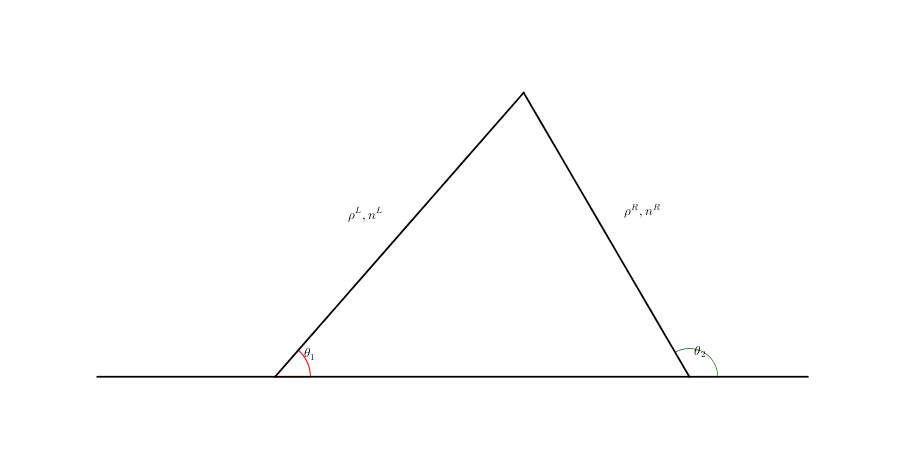
\includegraphics[width=\textwidth]{chapters/assets/dr/two-beam-line-model}
    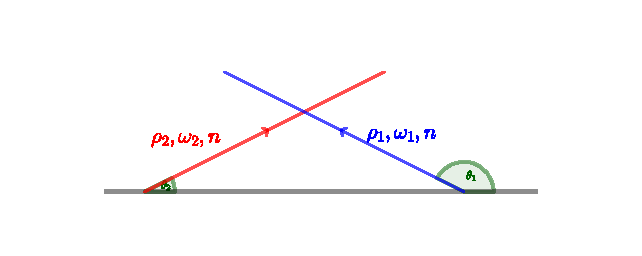
\includegraphics[width=\textwidth]{chapters/assets/collective/two-beams-model-sym}
    \caption{The geometry of two-beam model to be used in this section. The angles left-going beam contains neutrinos and the right-going beam contains antineutrinos. The corresponding emission angles are $\theta_1$ and $\theta_2$, respectively. }
    \label{chap:collective-sec:two-beams-fig:two-beam-line-model}
\end{figure}


The Hamiltonian of each beams becomes
\begin{align}
   \mathsf H_1 &= -\frac{1}{2} \omega_\vv \sigma_3 + \frac{1}{2} (\mu \rho_1 - \mu \rho_2), \\
    \mathsf H_2 &= \frac{1}{2} \omega_\vv \sigma_3 + \frac{1}{2} (\mu \rho_1 - \mu \rho_2),
\end{align}
where
\begin{align}
   \mu = \sqrt{2} G_{\mathrm F} \xi n
\end{align}
is the neutrino self-interaction potential and
\begin{equation}
    \xi =  1 - \cos(\theta_1 - \theta_2) 
\end{equation}
is the geometric factor.

This model is numerically solved and presented in Fig.~\ref{chap:collective-sec:two-beams-fig:two-beam-line-model-numerical-solution}. The neutrinos and antineutrinos are prepared to be in almost electron flavor but with a small perturbations
\begin{equation}
    \rho_i  = \frac{1}{2} \begin{pmatrix}
        1 & \epsilon_i \\
        \epsilon_i & -1
    \end{pmatrix},
    \label{chap:collective-sec:two-beams-eqn:density-matrix-perturbed}
\end{equation}
where $\epsilon_i$ is a small perturbation. I have removed the trace part because it is alway time independent in our model and commutes with the Hamiltonian.
For the numerical calculation, I have used $\epsilon_i = 10^{-3}$. In the beginning, the flavor isospin of the neutrino beam stays in the electron flavor state, i.e., in the direction of $s_3$ (see left panel of Fig.~\ref{chap:collective-sec:two-beams-fig:two-beam-line-model-numerical-solution}). It slowly deviates from the $s_3$ axes and rapidly falls down at some $z$. Then the flavor isospin comes back to its original position. The antineutrinos follow a similar pattern but is in a different direction. As shown in the right panel of  Fig.~\ref{chap:collective-sec:two-beams-fig:two-beam-line-model-numerical-solution}, the electron flavor is converted the other flavor in a way that is very different from the vacuum oscillations that I have showed in Fig.~\ref{chap:basics-section:neutrinos-fig:vacuum-2-flavor-osc}.

\begin{figure}[!htbp]
    \centering
    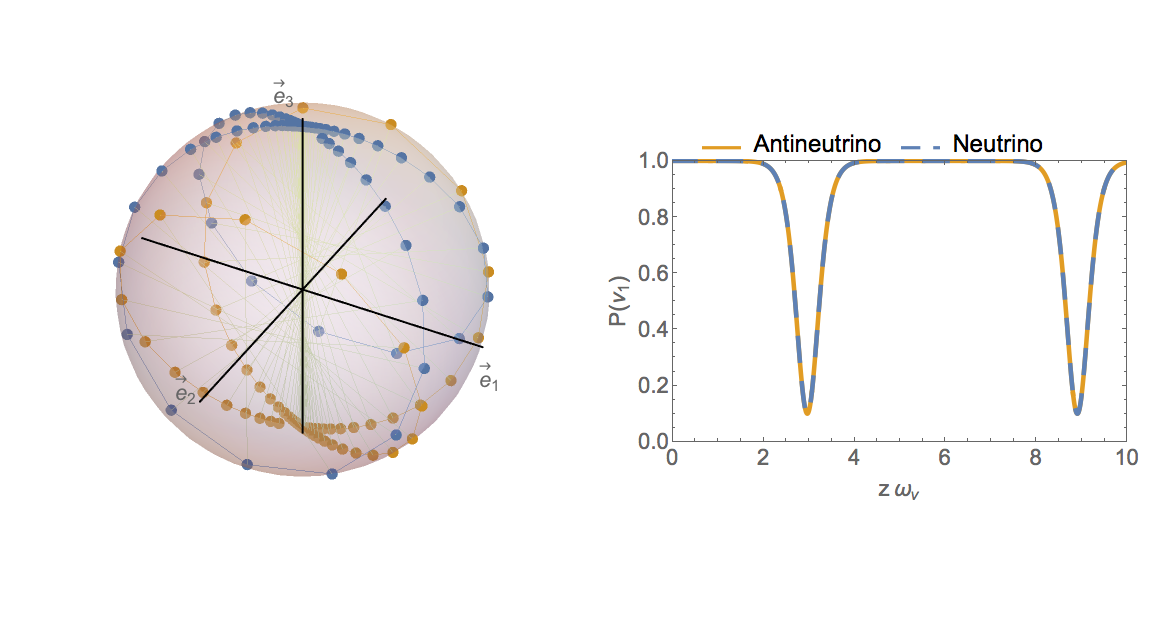
\includegraphics[width=\textwidth]{chapters/assets/collective/bipolar-animie100}
    \caption{The numerical solution to the two-beam model. The left panel shows the position of the flavor isospin of the neutrino beam and antineutrino beam. The right panel shows the electron flavor survival probabilities as a function of $z$ for both beams. The emission angles used in this calculation are $\theta_1=5\pi/6$ and $\theta_2=\pi/6$. The neutrino self-interaction potential is $\mu=5\lvert \omega_\vv\rvert$. }
    \label{chap:collective-sec:two-beams-fig:two-beam-line-model-numerical-solution}
\end{figure}

To analytically approach this problem, I will linearize the equation of motion and solve the neutrino flavor evolution in the linear regime. I start with the perturbed density matrix in Eqn.~\ref{chap:collective-sec:two-beams-eqn:density-matrix-perturbed} and plug it into the equation of motion. The linearized equation of motion is
\begin{equation}
    \ri \partial_z \begin{pmatrix}
        \epsilon_1 \\
        \epsilon_2
    \end{pmatrix} = \frac{1}{2} \begin{pmatrix}
        \mu + 2\omega_\vv & - \mu \\
        \mu & -2 \omega_\vv - \mu
    \end{pmatrix} \begin{pmatrix}
        \epsilon_1 \\
        \epsilon_2
    \end{pmatrix}.
\end{equation}
It can be solved by assuming a collective mode
\begin{equation}
    \begin{pmatrix}
        \epsilon_1 (z) \\
        \epsilon_2 (z)
    \end{pmatrix} = \begin{pmatrix}
        \epsilon_1 (0) \\
        \epsilon_2 (0)
    \end{pmatrix} e^{i K_z z},
    \label{chap:collective-sec:two-beams-eqn:equation-of-motion-collective-mode-assumption}
\end{equation}
where $K_z$ is the collective wave number of the neutrinos. The eigenvalues of the equation of motion gives the collective wave number
\begin{equation}
    K_z = \pm \sqrt{ \omega_\vv (\omega_\vv + \mu) }.
\end{equation}
When $\omega_\vv(\omega_\vv + \mu) < 0$, I obtain imaginary values for wave number $K_z$, which means that the perturbation will grow exponentially in $z$ direction. For normal hierarchy ($\omega_\vv > 0$), it requires
\begin{equation}
    \mu < -\omega_\vv < 0,
\end{equation}
which can not happen. Thus it is not possible to have flavor instability in normal hierarchy. On the other hand, flavor instabilities can occur in inverted hierarchy ($\omega_\vv$) when
\begin{equation}
    \mu > \lvert \omega_\vv \rvert.
\end{equation}



% The linearized equation of motion becomes
% \small\begin{align}
%    &\ri \partial_z \begin{pmatrix}
%    \epsilon_1 \\
%    \epsilon_2
%    \end{pmatrix} =  - i \begin{pmatrix}\cot\theta_1\partial_x & 0 \\
%    0 & \cot\theta_2 \partial_x
%    \end{pmatrix} \begin{pmatrix}
%    \epsilon_1 \\
%    \epsilon_2
%    \end{pmatrix} + \nonumber\\
%    &
%    \frac{1}{2}\begin{pmatrix}
%    (\lambda+ \mu_2 - \eta \omega_1 - \mu_2 \cos(\theta_1-\theta_2) )/\sin \theta_1 & -\mu_2 (1-\cos(\theta_1-\theta_2)) /\sin \theta_1\\
%    -\mu_1 (1- \cos(\theta_1-\theta_2))/\sin\theta_2 & (\lambda + \mu_1 - \eta \omega_2 - \mu_1 \cos(\theta_1-\theta_2) )/\sin\theta_2
%    \end{pmatrix}\begin{pmatrix}
%    \epsilon_1 \\
%    \epsilon_2
%    \end{pmatrix},
%    \label{chap:collective-sec:two-beams-eqn:line-model-two-beams-all-neutrino-linearized-eom}
% \end{align}\normalsize
% where
% \begin{align*}
%    \mu_1 =& \sqrt{2}G_F n_{t,1}\\
%    \mu_2 =& \sqrt{2}G_F n_{t,2}.
% \end{align*}



% \subsection{Left-right Symmetric Emission}


% We first consider a simple case, where $\theta_1=\pi-\theta_2\equiv\theta$, $\lambda=0$, $\eta=1$, and homogeneous in $x$ direction. For simplicity we define
% \begin{align*}
%    \mu =& \sqrt{2}G_F (n_1 + n_2)\\
%    \mu_i =& \mu \frac{n_i}{n_1+n_2}\equiv \mu f_i \\
%    \xi = & 1-\cos(\theta_1-\theta_2) \\
%    \omega'_i = & \lambda - \eta\omega_i.
% \end{align*}

% % I am aware that this is not a self-consistent example since $\theta_1=\theta_2$ indicates that $\xi=0$. As we will see, no instability is present in this case. However, we keep the term $\xi$ because we need to analyze the effect of symmetry breaking. This example builds up a formalism.

% The equation for perturbations becomes
% \begin{equation}
%    i\partial_z\begin{pmatrix}
%    \epsilon_1 \\
%    \epsilon_2
%    \end{pmatrix} = \frac{1}{2\sin\theta} \begin{pmatrix}
%    \omega'_1 + \mu f_2\xi & -\mu f_2 \xi \\
%    -\mu f_1 \xi & \omega'_2 + \mu f_1 \xi
%    \end{pmatrix}\begin{pmatrix}
%    \epsilon_1 \\
%    \epsilon_2
%    \end{pmatrix}.
%    \label{eqn-linearized-eom-symmetric-eg}
% \end{equation}
% Since $\mu$ is the most important energy scale in this problem, we scale all energies with it.
% \begin{equation}
%    i\partial_{\hat z}\begin{pmatrix}
%    \epsilon_1 \\
%    \epsilon_2
%    \end{pmatrix} = \frac{1}{2\sin\theta} \begin{pmatrix}
%    \hat\omega'_1 +  f_2\xi & - f_2 \xi \\
%    - f_1 \xi & \hat\omega'_2 +  f_1 \xi
%    \end{pmatrix}\begin{pmatrix}
%    \epsilon_1 \\
%    \epsilon_2
%    \end{pmatrix},
% \end{equation}
% where
% \begin{align*}
%    \partial_{\hat z} =& \frac{d}{\mu dz} \\
%    \hat \omega'_i =& \frac{\omega'_i}{\mu}.
% \end{align*}


% The characteristic equation for this equation is
% \begin{equation}
%    \left( ( \Omega - \hat\omega'_1 - f_2\xi )(\Omega - \hat\omega'_2-f_1\xi) - f_1 f_2 \xi^2 \right) =0,
%    \label{chap:collective-sec:two-beams-eqn:two-beam-line-characteristic-eqn-simple}
% \end{equation}
% which is simplified to
% \begin{equation*}
%    (\Omega-\Omega_1)(\Omega-\Omega_2) -f_1f_2\xi^2 = 0,
% \end{equation*}
% where
% \begin{align*}
%    \Omega_1 = & \hat\omega'_1 + f_2 \xi\\
%    \Omega_2 = & \hat\omega'_2 + f_1 \xi.
% \end{align*}
% Complete the square
% \begin{equation*}
%    (\Omega - (\Omega_1 + \Omega_2)/2)^2 = \frac{1}{4}(\Omega_1-\Omega_2) + f_1f_2\xi^2.
% \end{equation*}
% The solution becomes
% \begin{equation}
%    \Omega = \frac{1}{2}(\Omega_1+\Omega_2)\pm\sqrt{ (\Omega_1-\Omega_2)^2/4 + f_1f_2\xi^2 }.
% \end{equation}
% The condition to have positive imaginary part is
% \begin{equation*}
%    (\Omega_1-\Omega_2)^2 + 4f_1f_2\xi^2 < 0,
% \end{equation*}
% or
% \begin{equation*}
%    -2\sqrt{-f_1f_2\xi^2}<\Omega_1-\Omega_2<2\sqrt{-f_1f_2\xi^2},
% \end{equation*}
% and $f_1f_2\xi^2<0$. Recall the meaning of $f_i$,
% \begin{equation*}
%    f_i = \frac{n_i}{n_1+n_2},
% \end{equation*}
% instability requires that we have a spectrum crossing, i.e., $n_1$ and $n_2$ have different signs. Plug in the definitions of $\Omega_i$,
% \begin{equation*}
%    -2\sqrt{-f_1f_2\xi^2}< \eta(- \omega_1 + \omega_2)/\mu + (f_2 - f_1)\xi < 2\sqrt{-f_1f_2\xi^2}.
% \end{equation*}
% From this we can infer
% \begin{itemize}
%     \item $f_1f_2$ has to be negative, which means we can NOT have instabilities with only neutrinos or antineutrinos with all the symmetries we assumed. This is crossing.

% \item $-\omega_1+\omega_2=0$ will remove the instability. So we have to have both neutrinos and antineutrinos.
% \item $f_2-f_1$, $\eta(\omega_2-\omega_1)$, and $\mu$ set limit on each other.
% \item $\theta_1=\theta_2\equiv \theta$ removes the instability since it leads to $\xi=0$. The emission has to be asymmetric in this simple two beams model. This is trivial since equal emission angle means the beams are not colliding.
% \end{itemize}


% % .. admonition:: But why?
% %   :class: warning

% %   We have these conclusions. But why?

% %   What are the roles of

% %   1. :math:`f_i`,
% %   2. neutrino beam and antineutrino beam,
% %   3. hierarchy,
% %   4. neutrino number density variations,
% %   5. variations of angular distributions of neutrinos,
% %   6. variations of energy spectrum of neutrinos.


% Another way of understanding this equation is to think of it as the growth of the length of the vector $\vec v = (\epsilon_1,\epsilon_2)^T$. For an arbitrary matrix differential equation of the form
% \begin{equation*}
%   \partial_z \mathbf v = \mathbf A \mathbf v,
% \end{equation*}
% we can always decompose the matrix $\mathbf A$ into symmetric part and skew-symmetric part
% \begin{equation*}
%   \mathbf A = \frac{1}{2}(\mathbf A + \mathbf A^T) + \frac{1}{2}(\mathbf A - \mathbf A^T) \equiv \mathbf A^+ + \mathbf A^-.
% \end{equation*}
% We can identify the effect of $f_1-f_2$ but this is not particularly useful since we can not say anything about the eigenvalues of matrix $\mathbf A$ from the eigenvalues of matrix $\mathbf A^+$ and $\mathbf A^-$.



% \subsection{Breaking Symmetries}



% For a line model, the symmetries we have are
% \begin{itemize}
%     \item Time translation symmetry;
% \item Translation symmetry along the line;
% \item Energy spectrum of the beams; One of particular interest is to have different neutrino spheres for different energies which can be investigated using two beam model.
% \item Number density of left and right beams;
% \item Angle of left and right beams;
% \item With and without matter.
% \item Similar to the discussion of varying matter potential, symmetries can be broken globally, i.e., distribution as a function of spacetime coordinates.
% \end{itemize}

% I will discuss some of the symmetries mentioned above.



% \subsubsection{Emission Angle Parity Symmetry}

% The emission angles change the value of $\xi=1-\cos(\theta_1-\theta_2)$ as well as rescale the quantities by angle dependent factor $1/\sin\theta_i$.

% To see the importance of angles, we can redefine some quantities
% \begin{align*}
%    \omega''_i=& \frac{\omega'_i}{\sin\theta_i}\\
%    f''_1=&\frac{f_1}{\sin\theta_2} \\
%    f''_2=&\frac{f_2}{\sin\theta_1}.
% \end{align*}
% The we will reach the same characteristic equation as Eqn. \ref{chap:collective-sec:two-beams-eqn:two-beam-line-characteristic-eqn-simple}. So the angles serves as shift of energy gap and angular distribution.

% The region of instability changes in a convoluted way. Given angles we can always write down the expression and find out.
% \begin{itemize}
%     \item  The criteria of existence of instability doesn't change.
% \item  The region of instability changes.
% \end{itemize}


% \subsubsection{Matter Effect}


% Including matter will define vacuum frequencies, $\omega'_i$, which is effectively just a shift of vacuum frequencies. In the symmetric emission case, $\omega'_1-\omega'_2$ is independent of matter effect. But breaking the emission symmetry generates the degeneracy,
% \begin{equation}
%    \hat\omega''_1-\hat\omega''_2=( \lambda/\sin\theta_1 - \lambda/\sin\theta_2 + \eta(- \omega_1/\sin\theta_1 + \omega_2/\sin\theta_2) )/\mu`.
% \end{equation}

% We notice that very large matter density shift the region to very small $\mu$.

% However, matter effect is not always this simple. Suppose we have different matter potential for different beams, when they collide they would have built a different phase due to matter effect.

% The inhomogeneous matter effect has been studied in \cite{Mangano2014}. It can excite high Fourier moments of flavor-isospin picture, which makes a lot of sense because it generates fine structure in the x direction. This might be integrated into LESA effect.



% \subsubsection{Translation Symmetry}


% Translation symmetry is better explained by introducing Fourier transform in x direction.

% For each mode, a term that is proportional to Fourier mode index $m$. It only appears in diagonal elements, thus is effectively a shift of vacuum frequencies, thus energies of neutrinos.

% For each Fourier mode
% \begin{equation*}
%    \begin{pmatrix}
%    \epsilon_1 \\
%    \epsilon_2
%    \end{pmatrix} =  \mathbf Q(\Omega,k) e^{-i(\Omega t- k x)},
% \end{equation*}
% where we set $\Omega=0$.

% First term in RHS of Eqn.~ \ref{chap:collective-sec:two-beams-eqn:line-model-two-beams-all-neutrino-linearized-eom} becomes
% \begin{equation*}
%    - i \begin{pmatrix}\cot\theta_1\partial_x & 0 \\
%    0 & \cot\theta_2 \partial_x
%    \end{pmatrix} \begin{pmatrix}
%    \epsilon_1 \\
%    \epsilon_2
%    \end{pmatrix} = k \begin{pmatrix}\cot\theta_1 & 0 \\
%    0 & \cot\theta_2
%    \end{pmatrix} \begin{pmatrix}
%    Q_1 \\
%    Q_2
%    \end{pmatrix}.
% \end{equation*}
% We now define $\hat\omega''_i$, so that
% \begin{equation*}
%    \hat\omega''_{k,i} = \hat \omega''_i + 2\hat k\cot\theta_i,
% \end{equation*}
% where $\hat k=k/\mu$.

% The $k$ term contributes to the difference between $\Omega_{k,i}\equiv \hat\omega''_{k,i}+ f''_i\xi$.

% We notice that instability criteria doesn't change. However, the regime of instability changes. We also know that the instability region is determined by
% \begin{equation}
%    \lvert \Delta\hat\omega''_{12} + 2\hat k (\cot \theta_1 - \cot\theta_2) + \Delta f''_{12}\xi \rvert < \sqrt{-f_1f_2\xi^2},
% \end{equation}
% where $\Delta \hat \omega''_{12} = \hat\omega''_1-\hat\omega''_2$. The instability region shift from
% \begin{equation}
%    -\sqrt{-f''_1f''_2\xi^2} -\Delta f''_{12}\xi < (\Delta\omega''_{12} + 2 k(\cot\theta_1-\cot\theta_2))/\mu < \sqrt{-f''_1f''_2\xi^2} -\Delta f''_{12}\xi
% \end{equation}
% If $\lvert \Delta\omega''_{12} + 2 k(\cot\theta_1-\cot\theta_2) \rvert$ becomes larger, the region of instability is shifted to larger $\mu$, i.e., larger number density.



% \subsubsection{Number Density of Emission}


% A crossing is required to have instability, i.e., $-f''_1f''_2>0$. Meanwhile the number density on the left and right have little effects on the existence of instability. It shifts the region of instability for $\mu$.


% \subsubsection{Energy of Emission}



% Different energy of two beams will make sure $-\omega_1 + \omega_2\neq 0$. It has no effects on the criteria but changes the $\mu$ region of instability.


% % \subsubsection{Time Translation Symmetry}



% % .. admonition:: Time Translational Symmetry
% %   :class: warning

% %   How about time translational symmetry? I need to write down the equation of motion that is related to time.

% %   Two limits are of particular interest.

% %   1. Adiabatic limit,
% %   2. Superfast time variants.



% For completeness, I can also write down the linearized equation of motion without translational symmetries, c.f.~Eqn.~\ref{chap:collective-sec:two-beams-eqn:line-model-two-beams-all-neutrino-linearized-eom}. I know that real symmetric matrix has only real eigenvalues, from which I infer that $\mu_1=\mu_2$ and $\theta_1=\theta_2$ removes the instability.
% For translation symmetric models, that is $\partial_x\to 0$, I have the eigenvalues
% \begin{equation*}
%    \Omega = \frac{1}{4}(A\pm B),
% \end{equation*}
% where
% \begin{align*}
%    A=& -\eta \omega_1/\sin\theta_1 - \mu_2 /\sin\theta_1 + \eta \omega_2 /\sin\theta_2 + \mu_1 \xi /\sin\theta_2 + \lambda(1/\sin\theta_1 + 1/\sin\theta_2)  \\
%    B=& \left(
%       -4[(\lambda-\eta\omega_1)(\lambda +\eta\omega_2) + (\lambda (\mu_1-\mu_2) -\eta (\mu_1\omega_1 + \mu_2\omega_2) )\xi ] \sin\theta_1 \sin\theta_2\right. \\
%       &\left.+ [(\lambda + \eta\omega_2 + \mu_1\xi) \sin\theta_1 + (\lambda - \eta \omega_1 - \mu_2\xi) \sin\theta_2 ]^2
%    \right)^{1/2}/(\sin\theta_1\sin\theta_2)\\
%    \xi=&1-\cos(\theta_1-\theta_2).
% \end{align*}


% For antineutrinos, I only need to change $\mu_i\to -\bar\mu_i$ and $\omega_i\to -\bar\omega_i$, where $\bar\mu=\sqrt{2}G_F \bar n_t$, so that the equation becomes
% \small\begin{align*}
%   &i \partial_z \begin{pmatrix}
%   \epsilon_1 \\
%   \epsilon_2
%   \end{pmatrix} =  - i \begin{pmatrix}\cot\theta_1\partial_x & 0 \\
%   0 & \cot\theta_2 \partial_x
%   \end{pmatrix} \begin{pmatrix}
%   \epsilon_1 \\
%   \epsilon_2
%   \end{pmatrix} \\
%   &+
%   \frac{1}{2}\begin{pmatrix}
%   (\lambda-\bar\mu_2 + \eta \bar\omega_1 + \bar\mu_2 \cos(\theta_1-\theta_2) )/\sin \theta_1 & \bar\mu_2 (1-\cos(\theta_1-\theta_2)) /\sin \theta_1 \\
%   \bar\mu_1 (1- \cos(\theta_1-\theta_2))/\sin\theta_2 & (\lambda -\bar\mu_1 + \eta \bar\omega_2 +\bar\mu_1 \cos(\theta_1-\theta_2) )/\sin\theta_2
%   \end{pmatrix}\begin{pmatrix}
%   \epsilon_1 \\
%   \epsilon_2
%   \end{pmatrix}
% \end{align*}\normalsize

% Assume that the left beam is neutrino beam and the right beam is antineutrno beam. The linearized equation of motion becomes
% \small
% \begin{align*}
%   &i\partial_z \begin{pmatrix}
%   \epsilon_1 \\
%   \epsilon_2
%   \end{pmatrix} =  -i\begin{pmatrix}
%   \cot\theta_1 \partial_x & 0 \\
%   0 & \cot\theta_2 \partial_x
%   \end{pmatrix}\begin{pmatrix}
%   \epsilon_1 \\
%   \epsilon_2
%   \end{pmatrix} \\
%   &+ \frac{1}{2}\begin{pmatrix}
%   (\lambda - \bar\mu - 2\eta \omega_1 + \bar\mu \cos(\theta_1-\theta_2) )/\sin\theta_1 & \bar\mu (1-\cos(\theta_1-\theta_2))/\sin\theta_1 \\
%   -\mu(1-\cos(\theta_1-\theta_2))/\sin\theta_2 & (\lambda + \mu + \eta \omega_2 - \mu \cos(\theta_1-\theta_2) )/\sin\theta_2
%   \end{pmatrix}\begin{pmatrix}
%   \epsilon_1 \\
%   \epsilon_2
%   \end{pmatrix}
% \end{align*}
% \normalsize







\section{\label{chap:collective-sec:fast-mode}Fast Mode and Dispersion Relations}


The oscillation length scales of neutrino oscillations can be estimated by dimensional analysis. For example, the characteristic energy scale for vacuum oscillations is $\omega_{\mathrm v} = \delta m^2\big/2E $, which leads to neutrino oscillation frequency of the order
\begin{align*}
 \omega_{\mathrm v} = \frac{\Delta m^2}{2E}  \sim& \frac{2\pi}{ 1  \mathrm{km} }  \left(\frac{\Delta m^2_{32}}{2.5\times 10^{-3} \mathrm{eV}^2 } \right) \left( \frac{1MeV}{E} \right) \\
\sim & \frac{2\pi}{ 33  \mathrm{km} } \left( \frac{\Delta m_{12}^2}{7.5\times 10^{-5}\mathrm{eV}^2} \right) \left( \frac{1\mathrm{MeV}}{E} \right),
\end{align*}
where $E$ is the neutrino energy.
As for collective oscillations, suppose I have neutrino flux $10^{50}\mathrm{ergs\cdot s^{-1}}$. I can estimate the potential at radius $R$ to be
\begin{equation*}
\mu \sim  \frac{1}{0.01 \mathrm{km}} \left(\frac{100\mathrm{km}}{R}\right)^2 \left(\frac{1\mathrm{MeV}}{E}\right),
\end{equation*}
which means that the collective oscillations frequencies in supernova explosions can be much larger than the vacuum oscillations. The fast modes instability grows with a rate proportional to the neutrino potential $\mu=\sqrt{2}G_F n_\nu$, which is very large in dense neutrino media. In a paper by Chakraborty et al~\cite{Chakraborty2016}, they showed that neutrino oscillations in dense neutrino media can be much faster than than the vacuum oscillations.



% \subsection{\label{chap:collective-sec:fast-mode-subsec:introduction}Introduction}

% (Should talk about some very very basic backgrounds like the applications and why it is important.)





\section{\label{chap:collective-sec:fast-mode-subsec:dr}Dispersion Relation of Neutrino Flavor Conversion}

In this section, I will review the dispersion relations by following the paper by I. Izaguirre, G. Raffelt, and I. Tamborra~\cite{Izaguirre2016a}.

I assume that all neutrinos and antineutrinos are emitted as electron flavor. The flavor evolution of neutrino ensemble depends on flavor density matrices of neutrinos $\rho$ and antineutrinos $\bar\rho$ with energy $E$, direction of velocity $\hat{\mathbf v}$,
\begin{equation}
\ii (\partial_t + \mathbf v\cdot \mathbf{\nabla}) \rho = \left[H, \rho_n \right],
\label{eqn-liouville-eqn}
\end{equation}
where $H$ is the Hamiltonian for neutrino oscillations. In the context, Hamiltonian depends on three different contributions from vacuum oscillations $H_{\mathrm v}$, interactions with matter $H_{\mathrm m}$, and interactions with neutrinos themselves $H_{\nu\nu}$. In this work, we ignore vacuum and matter terms since the concentration is on fast neutrino oscillations, which would occur even without neutrino mass differences \cite{Chakraborty2016,Dasgupta2017}. In order to calculate the neutrino self-interaction term $H_{\nu\nu}$, the distribution of neutrinos (antineutrinos) $f_{\nu_{\mathrm e}(\bar \nu_{\mathrm e})}(\hat{\mathbf v}, E)$ and $f_{\nu_{\mathrm x}(\bar \nu_{\mathrm x})}(\hat{\mathbf v}, E)$ is required, where $E$ is the energy of neutrinos (antineutrinos). We have
\begin{equation}
H_{\nu\nu} = \sqrt{2} G_{\mathrm F} n \iint \dd \Gamma' v^\mu v'_\mu \int \frac{E'^2 \mathrm d E'}{2\pi^2} \left( (f_{\nu_{\mathrm e}}' - f_{\nu_{\mathrm x}}' )\rho' -  (f_{\bar\nu_{\mathrm e}}' - f_{\bar\nu_{\mathrm x}}' ) \bar\rho' \right),
\end{equation}
where $v^\mu = ( 1, \sin\theta\cos\phi, \sin\theta\sin\phi, \cos\theta )^{\mathrm T}$ is the four velocity of (anti)neutrinos in our spherical coordinate system, and $\dd \Gamma' = \frac{\mathrm d \cos\theta' \mathrm d\phi'}{4\pi}$. Without vacuum contribution, the equation of motion for antineutrinos has the same form \cite{Duan2010}.

I follow the same assumption in reference \cite{Izaguirre2016a} that the the distribution of $\nu_x$ and $\bar\nu_x$ are the same, namely $ f_{\nu_{\mathrm x}}({\mathbf v},E)  - f_{\bar\nu_{\mathrm x}}({\mathbf v},E)=0$. In addition, I have the same definition of electron lepton number (ELN) of neutrinos travelling in direction ${\mathbf v}$ \cite{Izaguirre2016a},
\begin{equation}
G({\mathbf v}) =  \sqrt{2}G_{\mathrm F} n \int \frac{E'^2 \mathrm d E'}{2\pi^2} ( f_{\nu_{\mathrm e}}(\cos\theta',\phi',E')  - f_{\bar\nu_{\mathrm e}}(\cos\theta',\phi',E')  ).
\end{equation}
To perform linear stability analysis, I assume that the density matrix has the form
\begin{equation}
\rho = \bar \rho = \frac{1}{2} \begin{pmatrix}
1 & \epsilon \\
\epsilon^* & -1
\end{pmatrix},
\end{equation}
where $\lvert \epsilon \rvert \ll 1$. Plug this into the equation of motion, I obtain the linearized equation of motion
\begin{align}
    \ri ( \partial_t + \mathbf v \cdot \boldsymbol{\nabla} ) \begin{pmatrix}
        1 & \epsilon \\
        \epsilon^* & -1
        \end{pmatrix}  =  \left[ -\omega_\vv\sigma_3 + \int \dd \Gamma' G(\mathbf v') v^\mu v'_\mu  \begin{pmatrix}
            1 & \epsilon' \\
            \epsilon'^* & -1
            \end{pmatrix} , \frac{1}{2}\begin{pmatrix}
            1 & \epsilon \\
            \epsilon^* & -1
            \end{pmatrix}\right],
\end{align}
which leads to the equation for the perturbation
\begin{equation}
    \ri ( \partial_t + \mathbf v \cdot \boldsymbol{\nabla} ) \epsilon = v^\mu \Phi_\mu \epsilon - \int \dd \Gamma' v^\mu v'_\mu G(\mathbf v') \epsilon',
    \label{chap:collective-sec:fast-mode-eqn:eom-continuous-general-linearized}
\end{equation}
where I have assumeed that all neutrinos and antineutrinos undergo the same behavior in linear regime, $\epsilon = \tilde\epsilon e^{-\ii (\Omega t - \mathbf K\cdot \mathbf x)}$. The four-potential in Eqn.~\ref{chap:collective-sec:fast-mode-eqn:eom-continuous-general-linearized}
\begin{equation}
    \Phi_\mu \to  \left( \int \dd \Gamma' G(\mathbf v'), \int \dd \Gamma' \mathbf v' G(\mathbf v') \right)^{\mathrm T}.
\end{equation}
With the equation of motion derived, I assume a collective mode 
\begin{equation}
\epsilon  \mathbf r = \tilde epsilon e^{- \ri (\Omega t - \mathbf K \cdot \mathbf r)},
\end{equation}
which is a generalization of Eqn.~\ref{chap:collective-sec:two-beams-eqn:equation-of-motion-collective-mode-assumption}. To get the equation of motion for the collective modes, I use the following substitution:
\begin{align}
    \epsilon & \to \tilde \epsilon, \\
    \partial_t & \to \ri \Omega, \\
    \boldsymbol{\nabla} & \to -\ri \mathbf K.
\end{align}
The equation of motion becomes
\begin{equation}
    v^\mu K_\mu \tilde \epsilon  = v^\mu \Phi_\mu \tilde \epsilon - \int \dd \Gamma' v^\mu v'_\mu G(\mathbf v') \tilde \epsilon',
\end{equation}
where $K_\mu \to (\Omega, \mathbf K)^{\mathrm T}$ is the four wave vector. I can combine $v^\mu K_\mu \tilde \epsilon$ and $v^\mu \Phi_\mu \tilde \epsilon$ by defining a new four wave vector
\begin{equation}
    k_\mu = K_\mu - \Phi_\mu.
\end{equation}
Following the convention of I. Izaguirre, I define the polarization tensor.
\begin{equation}
\Pi^\mu_{\phantom{\mu}\nu} = 1 + \int \frac{d\Omega}{4\pi} G(\theta,\phi) \frac{v^\mu v_\nu}{\omega- k \hat{\mathbf k}\cdot \hat{\mathbf v} },
\end{equation}
which defines the dispersion relation $\Pi^\mu_{\phantom{\mu}\nu} a^\nu = 0$, with $a^\nu = \int \frac{d\cos\theta' d\phi'}{4\pi} G(\hat{\mathbf v}') v^\nu \tilde\epsilon$. I find the nontrivial solutions by setting \cite{Izaguirre2016a},
\begin{equation}
\operatorname{det}\left( \Pi^\mu_{\phantom{\mu}\nu} \right) = 0.
\label{eqn-dr-determinant-equation}
\end{equation}


For simplicity, I consider axial symmetric neutrino emission so that Eq. \eqref{eqn-dr-determinant-equation} becomes
\begin{align}
&\det \left( \omega \mathrm{I} + \frac{1}{2}
\begin{pmatrix}
   I_0 & 0 & 0 & -I_1 \\
   0 & -\frac{1}{2} (I_0 - I_2) & 0 & 0 \\
   0 & 0 & -\frac{1}{2} (I_0 - I_2) & 0 \\
   I_1 & 0 & 0 & -I_2
\end{pmatrix}\right) \nonumber\\
&=0,
\label{eqn-det-polarization-tensor-axial}
\end{align}
where $\mathbf I$ is the rank 4 identity matrix and
\begin{equation}
   I_m =\int_{-1}^{1} d u G(u) \frac{u^m}{1 -  \left(\lvert k\rvert /\omega\right) u }.
\end{equation}
where we define $u=\cos\theta$. Eq. \eqref{eqn-det-polarization-tensor-axial} is equivalent to the result in reference \cite{Raffelt2013}. $\lvert k \rvert /\omega$ is defined as the refractive index $n$ of the flavor wave. For spectrum $G(u)$ without zero values, the forbidden region is given by $1 -  \left(\lvert k\rvert /\omega\right) u\leq 0$.

The dispersion relations can be categorized into two different types by symmetries. To incorporate azimuthal symmetry, I define solutions related to the first and second element of $a^\nu$ ($\nu=1,2$) to be multi-azimuthal angle (MAA) solutions since they are the only solutions that depend on azimuthal angle $\phi$. The other solutions which are related to $\nu=0,3$ are defined to be the multi-zenith angle (MZA) solutions. The MAA solution is related to symmetry breaking in azimuthal angle only, which is determined by
\begin{equation}
   \omega = \frac{1}{4}(I_0 - I_2).
   \label{eqn-maa}
\end{equation}
Similarly, the MZA solution is related to symmetry breaking in both azimuthal angle and zenith angle, which is
\begin{equation}
\omega = - \frac{1}{4} \left( I_0 - I_2 \pm \sqrt{ (I_0 + I_2 - 2 I_1) (I_0 + I_2 + 2 I_1) } \right).
\label{eqn-mza}
\end{equation}
I denote the solution associated with $+$ sign in Eq. \eqref{eqn-mza} as MZA+, while the solution assocated with $-$ sign as MZA-. The two solutions are connected to each other in dispersion relations. In general, it doesn't provide physical insights to distingush the two branches of solutions since they are simply two branches of the solution.

The solutions to Eq. \eqref{eqn-maa} and Eq. \eqref{eqn-mza} are dispersion relations $D(\omega,\mathbf k)$ for a chosen direction of $\hat{\mathbf k} = \hat{\mathbf z}$ with axial symmetric neutrino emission.



%%%%%%%%%%%%%%%%%
%% To BE Added
%%%%%%%%%%%%%%%%
% {\color{red}{\bf HAVE TO EXPLAIN THE IDEA OF GAP AND INSTABILITY HERE. Maybe Later?}}






\section{\label{chap:collective-sec:fast-mode-subsec:instabilities-and-gaps}Instabilities and Gaps}

In reference \cite{Izaguirre2016a}, the authors relate gaps in dispersion relation to instabilities of neutrino oscillations. In this section, I review the idea of correspondence betIen gaps and instabilities first. Then I show that this relation is not a solid theory that can be generalized to all cases.

I continue the discussion of axial symmetric neutrino emissions but with discretized zenith angles $\theta$ thus discretized $u$. Hence the ELN is independent of azimuth angle $\phi$. For neutrino emission with $2$ zenith angles, the ELN spectrum is
\begin{equation}
G(u)= \sum_{i=1}^2 g_i \delta(u - u_i).
\end{equation}

The MAA solution becomes an equation of hypobola for $\omega$ and $k$, which has asymptotes $\omega = k u_i$ for $i=1,2$. Meanwhile, hyperbola equation has two solutions of $\omega$ ($k$) for any given real $k$ ($\omega$). The solutions are either real which indicates stable solutions or complex which indicates exponential growth or decrease in linear regime. On the other hand, non-existence of real solutions of $\omega$ ($k$) for given real $k$ ($\omega$) is equivalent to gap in dispersion relation. Thus the equivalence of gap and instabilities is guaranteed in neutrino emission with two-zenith-angle emission. The numerical calculations is normalized using the maximium value in spectrum which is a convention I follow for all discrete emission calculations. Unit for $\omega$ and $k$ can be determined once the exact spectrum is determined. Upper panels of Fig. \ref{fig-dr-db} is reproduction of left panels of Fig. 1 in reference \cite{Izaguirre2016a}. The dispersion relation is shown as black lines. The real part $\omega_{\mathrm R}$ is shown as red solid lines. $\omega_{\mathrm R} \pm \omega_{\mathrm I}$ are shown are red dashed lines, where $\omega_{\mathrm I}$ is the imaginary part of $\omega$.



\begin{figure}[!htb]
\minipage{0.49\textwidth}
  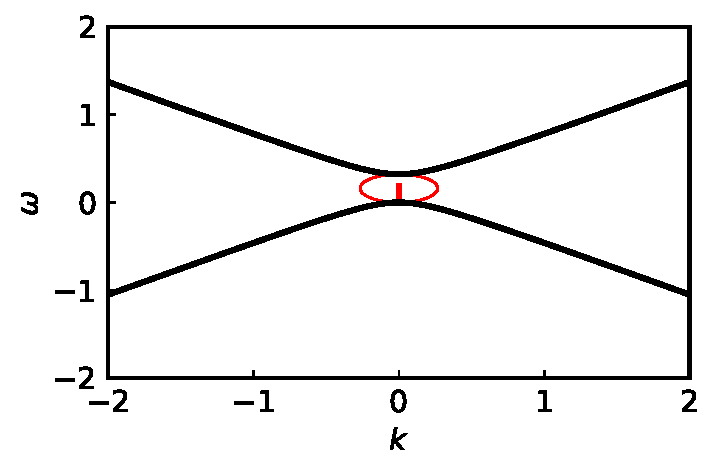
\includegraphics[width=\linewidth]{chapters/assets/dr/spectDBWC1DRDBMAAPltBlob.pdf}
\endminipage\hfill
\minipage{0.49\textwidth}
  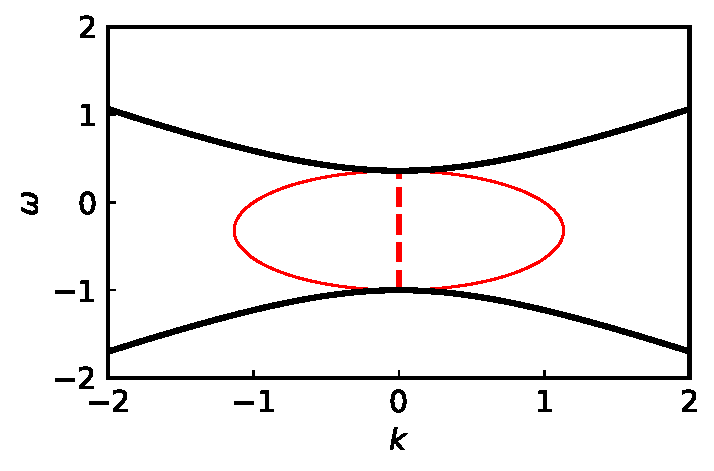
\includegraphics[width=\linewidth]{chapters/assets/dr/spectDBWC1DRDBMZAPltBlob.pdf}
\endminipage\hfill
\newline
\minipage{0.49\textwidth}
  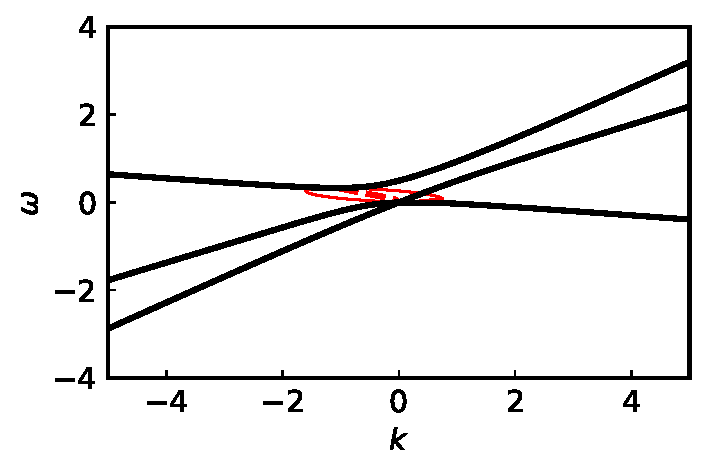
\includegraphics[width=\linewidth]{chapters/assets/dr/spectDB3WC4DRDBMAAPltBlob.pdf}
\endminipage\hfill
\minipage{0.49\textwidth}
  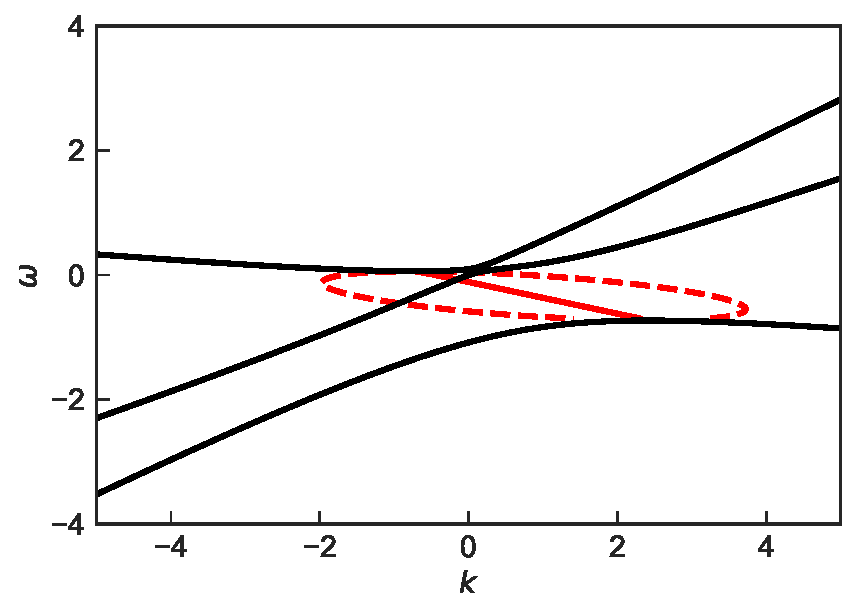
\includegraphics[width=\linewidth]{chapters/assets/dr/spectDB3WC4DRDBMZAPltBlob.pdf}
\endminipage\hfill
\caption{Dispersion relation and instabilities of two zenith angles spectrum (upper panels) and three zenith angles spectrum (loIr panels). The black lines are the dispersion relations and the colored dots are examples of complex $\omega$ for real $k$. The left panels are the dispersion relation and linear stability analysis of MAA solutions while the right panels are for MZA solutions.}
\label{fig-dr-db}
\end{figure}



In core collapse supernova and neutron star mergers, neutrino emission is not in discrete zenith angles. More realistic models involve continuous zenith angle ELN spectra. In the case that the smooth and continuous ELN spectrum has no crossing, gap indeed indicates instabilities, as shown in reference \cite{Izaguirre2016a}. In this section I prove that the instabilities in MAA, MZA+, or MZA- solution can only appear in either region $\omega\leq 0$ or region $\omega \geq 0$. As it suggests, the instability regions propagate only betIen the dispersion relation curves and the axis $\omega=0$. I reproduced the calculation in reference \cite{Izaguirre2016a} using the same Garching core-collapse supernova data set \cite{garching-ccsn-data}. The spectrum shown in the left panel of Fig. \ref{fig-garching} is polynomial fitting of the Garching 1D supernova simulation data. On the right of Fig. \ref{fig-garching}, the dispersion relation for MAA (MZA) solution is shown as red (green, blue) solid lines. Instabilities associated with MAA (MZA) solution is shown as light red (light green, light blue) blobs. The two branches of MZA solutions appear at the top half (MZA+) and lower half (MZA-). The result shows that instabilities occur either in region $\omega>0$ or region $\omega<0$ and with limits set the dispersion relation. Iwill prove that the instabilities appear between the dispersion relation and the axis $\omega=0$.






\begin{figure}
   \minipage{0.49\textwidth}
     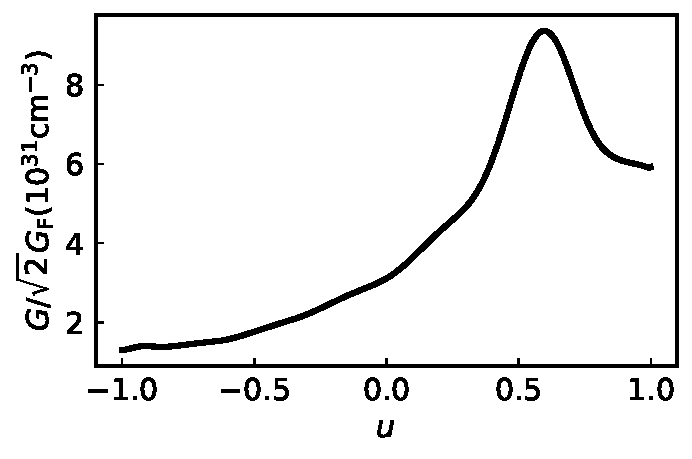
\includegraphics[width=\linewidth]{chapters/assets/dr/spectGarchingPlt.pdf}
   \endminipage\hfill
   \minipage{0.49\textwidth}
   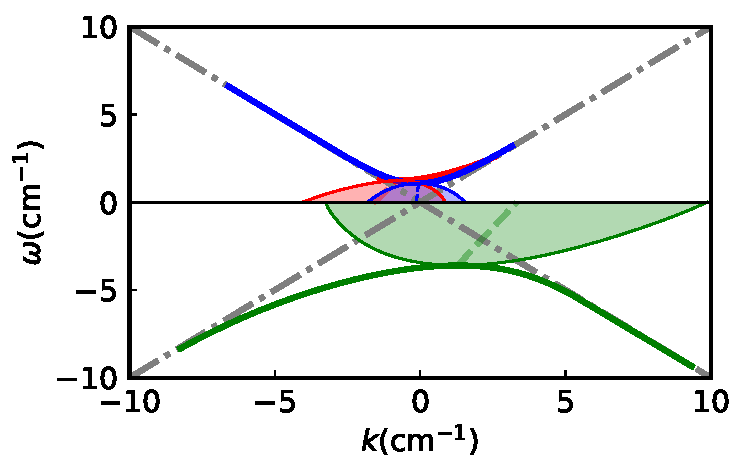
\includegraphics[width=\linewidth]{chapters/assets/dr/spectGarchingDRLSAPltBlob.pdf}
   \endminipage\hfill
   \caption{Dispersion relation and linear stability analysis (right panel) for a spectrum constructed from Garching 1D simulation data (left panel). Solid red line is dispersion relation for MAA solution while blue and green lines are for MZA solutions. Light red (green and green) blob is instability for MAA (MZA) solution.
    }
   \label{fig-garching}
\end{figure}




% \subsection{\label{sec-omega-to-zero}Instabilities at $\omega\to 0$}

Suppose I am looking for complex solutions for given real omega as in Fig. \ref{fig-garching}, MAA solution Eq. \eqref{eqn-maa} is rewritten as a function $k(\omega/k)$. More explicitly, I have to solve the integral function to find out $k$ for real $\omega$,
\begin{equation}
   k = \frac{1}{4} \int \mathrm du G(u) \frac{ 1 - u^2 }{ \omega/k - u }.
   \label{eqn-k-omega-relation}
\end{equation}
To investigate how instabilities developed around the horizental axies, I solve Eq. \eqref{eqn-k-omega-relation} in the limit $\omega\to 0$. For complex $k$, the integral can be decomposed into the principal value $\operatorname{Re}(k)$ and imaginary part $\operatorname{Im}(k)$ using Sokhotski–Plemelj theorem,
\begin{subequations}
\begin{align}
\operatorname{Re}(k) =& \frac{1}{4}\left(  \mathcal{P} \int \mathrm d u G(u) \frac{ 1 - u^2 }{ - u }  \right)\label{eqn-re-k-arbitrary-spectrum} \\
\operatorname{Im}(k) =&  \frac{\pi}{4}G(0) \operatorname{Sign}\left( \omega \right) \operatorname{Sign}\left(  \operatorname{Im}(k)  \right).
\label{eqn-im-k-arbitrary-spectrum}
\end{align}
\end{subequations}
Assuming no crossing is found in sepctrum $G(u)$ at $u=0$, Eq. \eqref{eqn-im-k-arbitrary-spectrum} shows that $\omega$ must have the same sign as $G(0)$ if I find nonzero imaginary part in $k$. I conclude that instabilities can only grow either in the upper plane $\omega>0$ or lower plane $\omega<0$. What's more, the value of $k$ at limit $\omega\to 0$ can be solved out of Eq. \eqref{eqn-re-k-arbitrary-spectrum} and Eq. \eqref{eqn-im-k-arbitrary-spectrum}. For instabilities the imaginary part of $k$ tells us the growth rate is,
\begin{equation}
   \lvert \operatorname{Im}(k) \rvert  =  \frac{\pi}{4}\lvert G(0)\rvert .
\end{equation}
Similar result is obtained for MZA solutions,
\begin{align}
&\left(4\operatorname{Re}(k) - \mathcal P \int \frac{G(u)}{u} \mathrm d u + U_1 \right)^2  - \left( \operatorname{Sign}(\omega \operatorname{Im}(k) )\pi G(0) +4 \operatorname{Im}(k) \right)^2 \\
% =&\left( \mathcal P \int \frac{G(u)}{u} \mathrm d u + U_1 \right)^2 -1 - 4 U_0^2  \\
% &\left( 4 \operatorname{Re}(k) - \mathcal P \int \frac{G(u)}{u} \mathrm d u + U_1 \right) \left( \pi \operatorname{Sign}(\omega \operatorname{Im}(k) ) G(0) + 4 \operatorname{Im}(k) \right) \\
=& - \left( \mathcal P \int \frac{G(u)}{u} \mathrm du + U_1 \right) \pi \operatorname{Sign}(\omega \operatorname{Im}(k) ) G(0),
\end{align}
where $U_m = \int G(u) u^m \mathrm du$ and all the integrals are over all the sepctrum. The equations are quadratic in both $\operatorname{Re}(k)$ and $\operatorname{Im}(k)$ so the real solutions can be calculated and verified with linear stability analysis. The imaginary part $\operatorname{Im}(k)$
\begin{equation}
   \operatorname{Im}(k) = - \frac{1}{4} \pi G(0) \operatorname{Sign}(\omega \operatorname{Im}(k) ) \left(  1 \pm \frac{ \mathscr P \int \frac{G(u)}{u} du + \int G(u) u du }{ 4 \operatorname{Re}(k) - \mathscr P \int \frac{G(u)}{u} du + \int G(u) u du }  \right)
\end{equation}
determines that the two different solutions are either in the region $\omega>0$ or in the region $\omega<0$ which corresponds to MZA+ and MZA- solutions. The instabilities in the two regions are not continuous at $\omega=0$.



\subsection{\label{chap:collective-sec:fast-mode-subsec:instability-to-gap}Instabilities Do Not Always Show Up as Gap}

Even though the concept of gap leads to instabilities works well for the models in \ref{chap:collective-sec:fast-mode-subsec:instabilities-and-gaps}, it can not be generalized to arbitrary number of emission angles nor to continuous spectra with crossings. As an example, I perform linear stability analysis of the three zenith angles emission configuration which is determined by a cubic function both in $\omega$ and $k$. Three solutions of $k(\omega)$ for given real $\omega(k)$  are expected. As long as real solutions disappear, complex solutions emerge, which leads to instabilities occur even without an actual gap. Rather the decrease in the number of real solutions for fixed $\omega$ or $k$ corresponds to the instabilities. As an example, I plotted dispersion relation and instabilities for three zenith angles in lower panels of Fig. \ref{fig-dr-db}. For a given value of $\omega$ such as $\omega= 0.5$, the three MAA solutions (Fig. \ref{fig-dr-db} lower left panel) of $k$ are $k=-4.6, 0.29, 1.2$. All three solutions are all real and indicate no spatial instabilities which is confirmed by calculation of instabilities shown as red blob. However, for another real $\omega = 0.2$, I find only one real solution $k=0.4$ from dispersion relation. The other solutions are complex and proven to be $k = -0.557106\pm 0.966535\mathrm i$ where the value with positive imaginary part leads to exponential growth. I conclude that instabilities doesn't require gap in dispersion relation except for two emission angles.


I will prove that instabilities for continuous emission angles do not necessarily correspond to gap in dispersion relation. In the earlier works of fast modes, Sawyer analyzed a box shaped angular distribution of neutrino emission \cite{Sawyer2016}. To address the generality of our conclusion, I repeat the calculation for box spectrum with crossing.

I construct a box spectrum with value $-0.1$ within $u\in [-1,-0.3)$ and value $1$ within $[-0.3,1]$ as shown in the top left panel of Fig. \ref{fig-box-c1}. As in the discrete emission case, I normalize all quantities using the maximium value of the spectrum. With the spectrum defined, I calculate the dispersion relation and find out complex values of $k$ for real $\omega$. The result shows that the dispersion relation of both MAA solution and MZA solution contains only one curve. No gap is formed but I observe instabilities between this curve and $\omega=0$ in MAA solution as well as two unstable regions of $k$ in MZA solution, which are plotted as red lines.


\begin{figure}
   % \minipage{0.49\textwidth}
   %   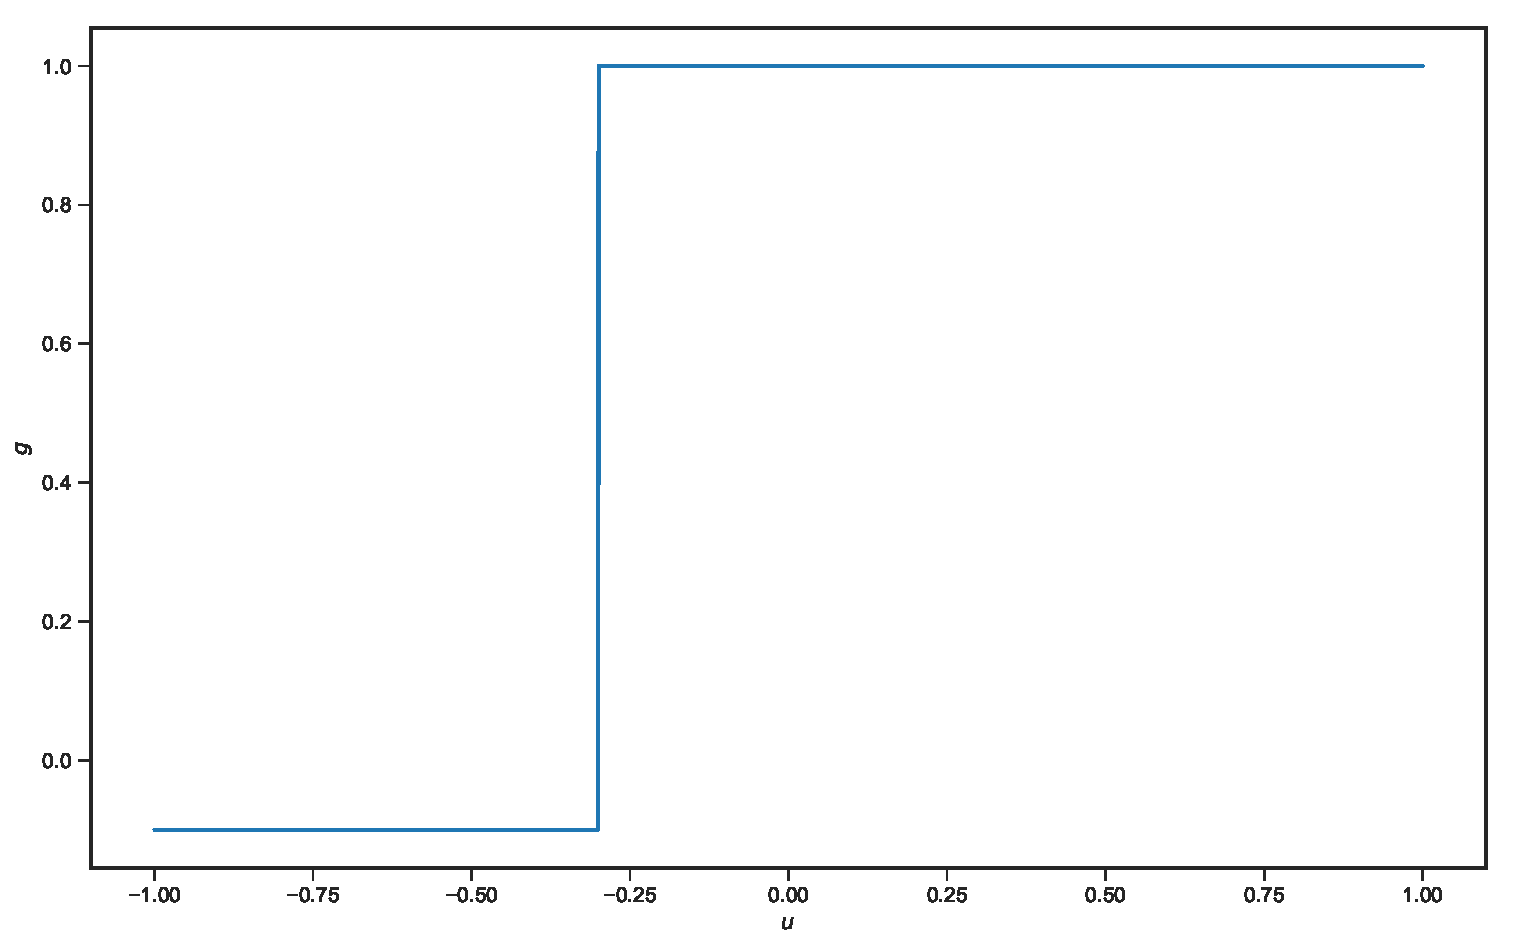
\includegraphics[width=\linewidth]{chapters/assets/dr/spectBoxC1Spectrum.pdf}
   % \endminipage\hfill
   \minipage{0.49\textwidth}
   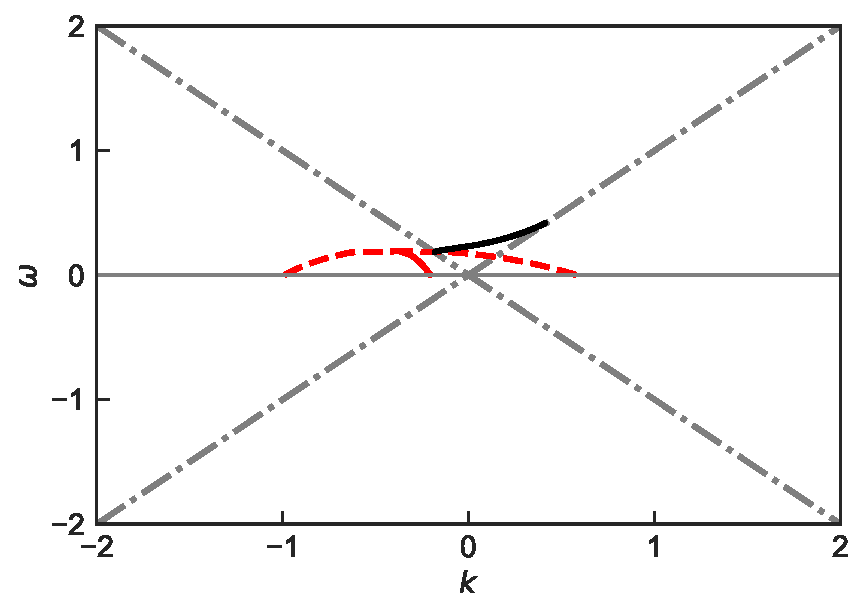
\includegraphics[width=\linewidth]{chapters/assets/dr/spectBoxC1MAADRPltBlob.pdf}
   \endminipage\hfill
   \minipage{0.49\textwidth}
   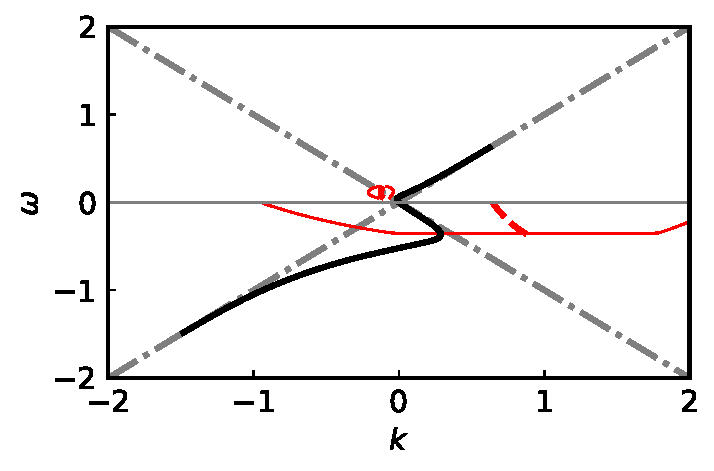
\includegraphics[width=\linewidth]{chapters/assets/dr/spectBoxC1MZADRPltBlob.pdf}
   \endminipage\hfill
   \caption{Dispersion relation and linear stability analysis for box spectrum. The box spectrum is defined to be $-0.1$ within range $u\in [-1,-0.3)$ and $1$ within range $u\in [-0.3,1]$. Left panel shows the dispersion relation and the complex $k$ for real $\omega$ for MAA solution. Right panel is the corresponding result for MZA solution. Dash-dotted gray lines are $\omega= \pm k$ which sets the boundaries of the forbidden region for dispersion relation.
    }
   \label{fig-box-c1}
\end{figure}



%%%%%%%%%%%%%%%%%%%%%%%%%%%%%%%%%%%%%%%%%%%%%%%%%%%%%%%%%%%%%%%%%%%%%%%%%
%%%%%%%%%%%%%%%%%%%%%% Neutrino Halo Problem %%%%%%%%%%%%%%%%%%%%%%%%%%%%
%%%%%%%%%%%%%%%%%%%%%%%%%%%%%%%%%%%%%%%%%%%%%%%%%%%%%%%%%%%%%%%%%%%%%%%%%





\section{\label{chap:halo}Neutrino Halo Problem}


One of the big questions about neutrino oscillations in supernovae is the so called halo problem. Cherry et al showed that neutrino flavor conversions are greatly affected by the back scattered neutrinos in supernovae~\cite{Cherry2012}. Neutrinos around supernovae are scattered and some of them are scattered to move almost backward. On the other hand, neutrino self-interactions is proportional to the inner product of momenta of neutrinos, which leads to the dependence on $1-\cos\theta$ where $\theta$ is the angles between momenta of two neutrinos. Most of the research has been concentrating on mostly forward scattering, with small values for $1-\cos\theta$. For back ward scattered neutrinos, the interaction potential can be much larger than the forward scattered neutrino contributions. Though the work by Sarikas et al showed that matter suppression is still significant within this region~\cite{Sarikas2012a}, it is not clear how exactly the neutrino halo alters neutrino oscillations. The halo problem itself is worth more calculations. In this chapter, I will present a relaxation method for this problem. The focus will be on the numerical method itself.


\subsection{\label{chap:halo-sec:line}Line Model}

I continue to use the simplified line model and build our intuitions out of it. The halo problem is simplified to have neutrinos emitted from a line $z=0$ homogeneously, which are reflected from a certain distance $z=L$. In principle, the reflection angles doesn’t have to be Snell’s law. The scattering can be in any angle with different amplitudes. Here I am using this very simple Snell’s law just to explore the effect of halo. It's crucial to keep an eye on the simplifications in this line model.
\begin{itemize}
    \item Neutrinos are emitted from a line, which is not the case in a real supernova.
    \item Neutrinos are emitted with translation symmetry on the line. Breaking the symmetry might bring in other qualitatively different results.
    \item Neutrinos are reflected from a certain surface $z=L$, which is different from reality where neutrinos are scattered everywhere.
    \item Neutrinos are reflected according to Snell's law.
    \item Neutrinos are homogeneously reflected at $z=L$.
\end{itemize}



\begin{figure}
    \centering
    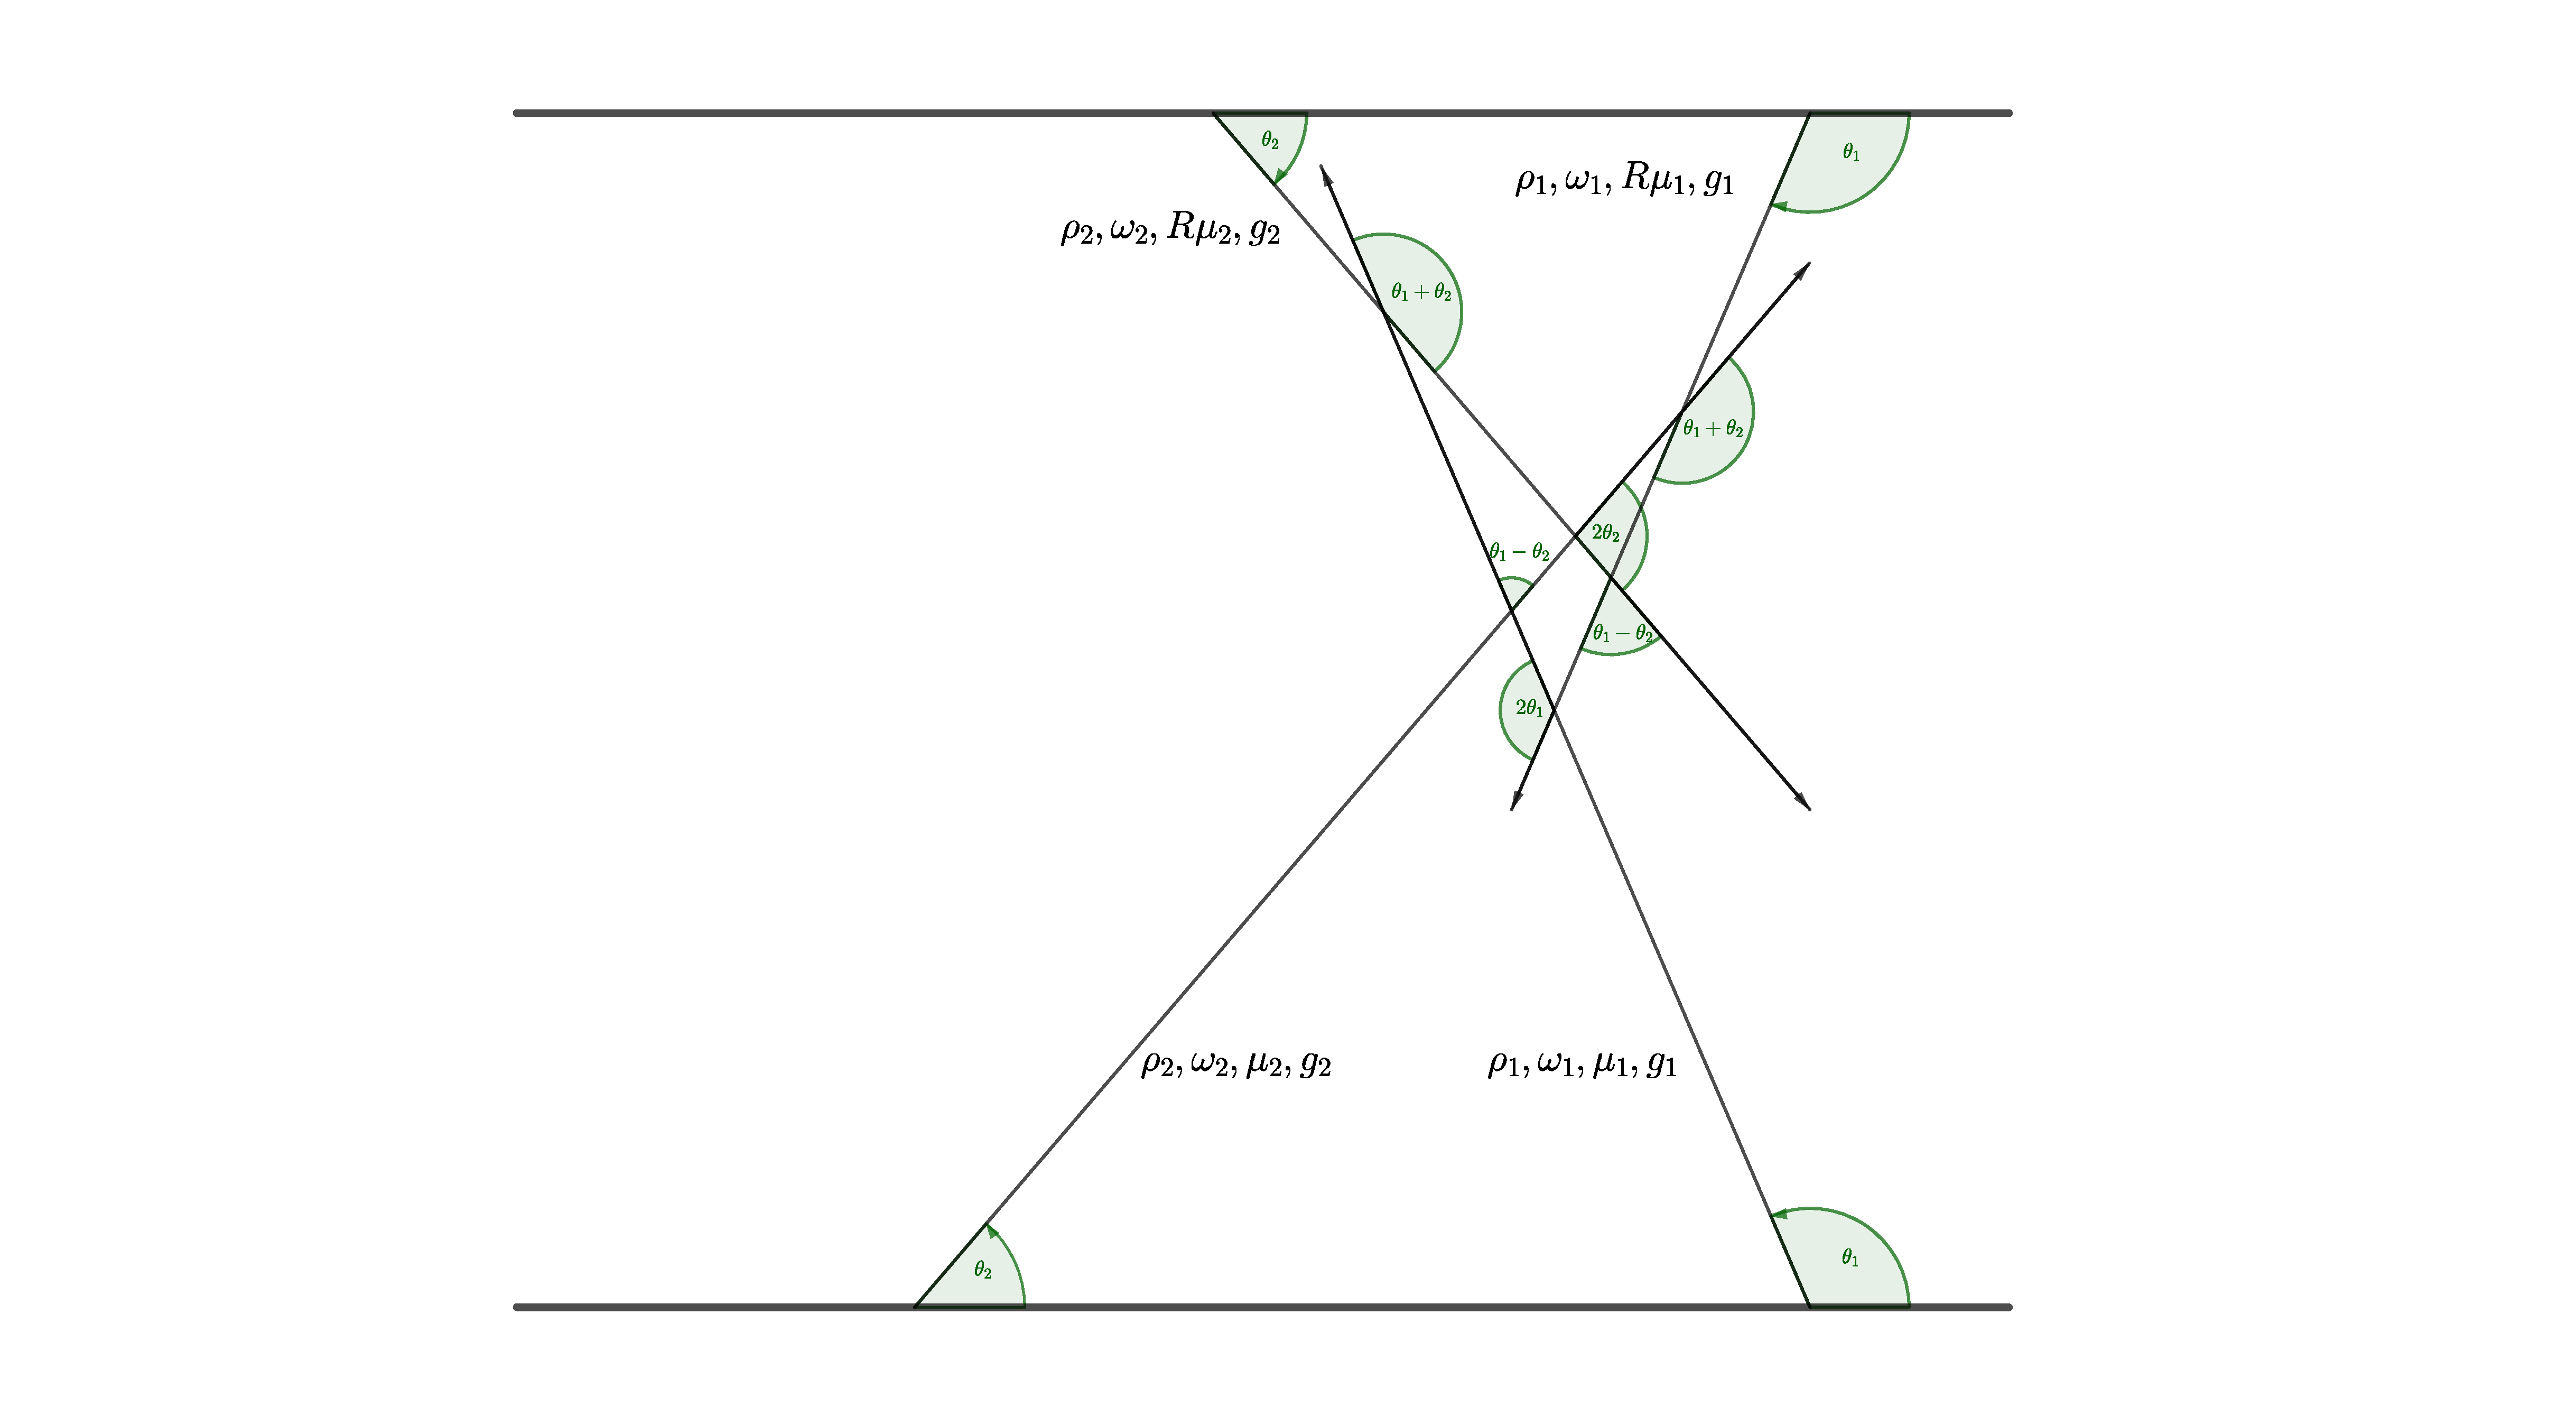
\includegraphics[width=\textwidth]{chapters/assets/halo/line-model.pdf}
    \caption{Line model used for halo problem. Neutrinos are emitted from the bottom line and reflected at the top line. Two neutrino beams are demonstrated in the figure. The beams are reflected from a surface at $z=L$.}
    \label{chap:halo-sec:line-fig:line-model}
\end{figure}


The algorithm that I used is relaxation method. The algorithm is meant to find the equilibrium state of neutrino oscillations with the presence of halo.
\begin{enumerate}
\item Calculate forward beam using 0 backward beam;
\item Calculate backward beam using forward beam calculated in 1;
\item Calculate forward beam using backward beam calculated in 2;
\item Repeat until the beams reach equilibrium.
\end{enumerate}


\subsection{\label{chap:halo-sec:line-sym}Neutrino Beams Only}

As a first step, I calculated neutrino oscillations with only neutrino beams. Before I rush to the numerical results, I linearized the equation of motion and worked out the linear stability analysis.

In linear regime, I define the density matrices for forward and backward beams to be
\begin{align*}
   \rho_F &= \frac{1}{2} \begin{pmatrix}
   1 & \epsilon_F \\
   \epsilon_B^* & -1
   \end{pmatrix} \\
   \rho_B &= \frac{1}{2} \begin{pmatrix}
   1 & \epsilon_B \\
   \epsilon_B^* & -1
   \end{pmatrix}.
\end{align*}
The Hamiltonian for forward and back ward beams are
\begin{align*}
   H_F &= H_v + R \mu \rho_B \\
   H_B &= H_v + \mu \rho_F.
\end{align*}
I will investigate the instability for zero mixing angle for new instabilities. The linearized equation of motion can be simplified to
\begin{align*}
   i\partial_z \begin{pmatrix}
   \epsilon_F \\
   \epsilon_B
   \end{pmatrix} = \begin{pmatrix}
   -\omega_v + R \xi \mu & - R \xi \mu \\
   \xi \mu & \omega_v - \xi \mu
   \end{pmatrix} \begin{pmatrix}
   \epsilon_F \\
   \epsilon_B
   \end{pmatrix}.
\end{align*}
This equation can be easily solved. The eigenvalues are
\begin{align*}
   \Omega_+ &= \frac{1}{2} ( (R-1)\xi\mu + \sqrt{\Delta} ) \\
   \Omega_- &= \frac{1}{2} ( (R-1)\xi\mu - \sqrt{\Delta} ),
\end{align*}
where
\begin{equation}
   \Delta = (1-R)^2 \mu^2 \xi^2 - 4\mu\xi \omega_v (1+R) + 4\omega_v^2.
\end{equation}
The corresponding eigenvectors are
\begin{align*}
   V_+ &=\begin{pmatrix}
   \frac{ -2\omega_v + \xi \mu (1+R) + \sqrt{\Delta} }{2\xi\mu} \\
   1
   \end{pmatrix} \\
   V_- &=\begin{pmatrix}
   \frac{ -2\omega_v + \xi \mu (1+R) - \sqrt{\Delta} }{2\xi\mu} \\
   1
   \end{pmatrix}.
\end{align*}
The general solution to the equation is
\begin{equation*}
   \begin{pmatrix}
   \epsilon_F(z) \\
   \epsilon_B(z)
   \end{pmatrix} = C_+ V_+ e^{-i \Omega_+ z} +  C_- V_- e^{-i \Omega_- z}.
\end{equation*}

The special property about this reflection problem is that the density matrices for the forward and backward beams should be the same at the reflection point, say $z=L$. With such a simple relation, we can find the relations between $C_\pm$ by setting $\epsilon_F(L)=\epsilon_B(L)$,
\begin{equation}
   \frac{C_+}{C_-} = e^{-i(\Omega_- -\Omega_+)L} \frac{ \sqrt{\Delta} +  2\omega_v + \mu \xi (1-R) }{\sqrt{\Delta} -  2\omega_v - \mu \xi (1-R)}.
\end{equation}
The solution to be problem can be simplified,
\begin{equation}
   \begin{pmatrix}
   \epsilon_F(z) \\
   \epsilon_B(z)
   \end{pmatrix} = C_- e^{-i\Omega_- L} \left( \frac{ \sqrt{\Delta} +  2\omega_v + \mu \xi (1-R) }{\sqrt{\Delta} -  2\omega_v - \mu \xi (1-R)} V_+ e^{-i \Omega_+ (z-L)} +  V_- e^{-i \Omega_- (z-L)} \right).
\end{equation}

I am interested in the absolute values of each elements so that the overall factors can be neglected. The forward beam evolution is obtained by taking the absolute value of $\epsilon_F$,
\begin{align*}
   \left\vert \epsilon_F \right\vert \propto & \lvert (2\omega_v +\xi\mu(1-R) +i \delta ) ( -2\omega_v + \xi\mu(1+R) + i \delta ) e^{\delta(z-L)} \\ 
   &+ ( -2\omega_v - \xi\mu(1-R) +i \delta ) ( -2\omega_v + \xi\mu(1+R) - i \delta ) e^{-\delta(z-L)} \rvert,
\end{align*}
in which $\sqrt{\Delta}$ is replaced by $i \delta$. I collect terms and verify that it has the form
\begin{equation}
   \left\vert \epsilon_F \right\vert \propto A + B \cosh( 2\delta(L-z) ),
\end{equation}
where $B\leq 0$.
The only $z$ dependent term is $\cosh( 2\delta(L-z) )$, which is decreasing within $[0,L]$ and is increasing in $[L,2L]$. The slope at $z=L$ is 0. An example is plotted in Fig.~\ref{chap:halo-sec:line-sym-fig:cosh}.


\begin{figure}[!htbp]
    \centering
    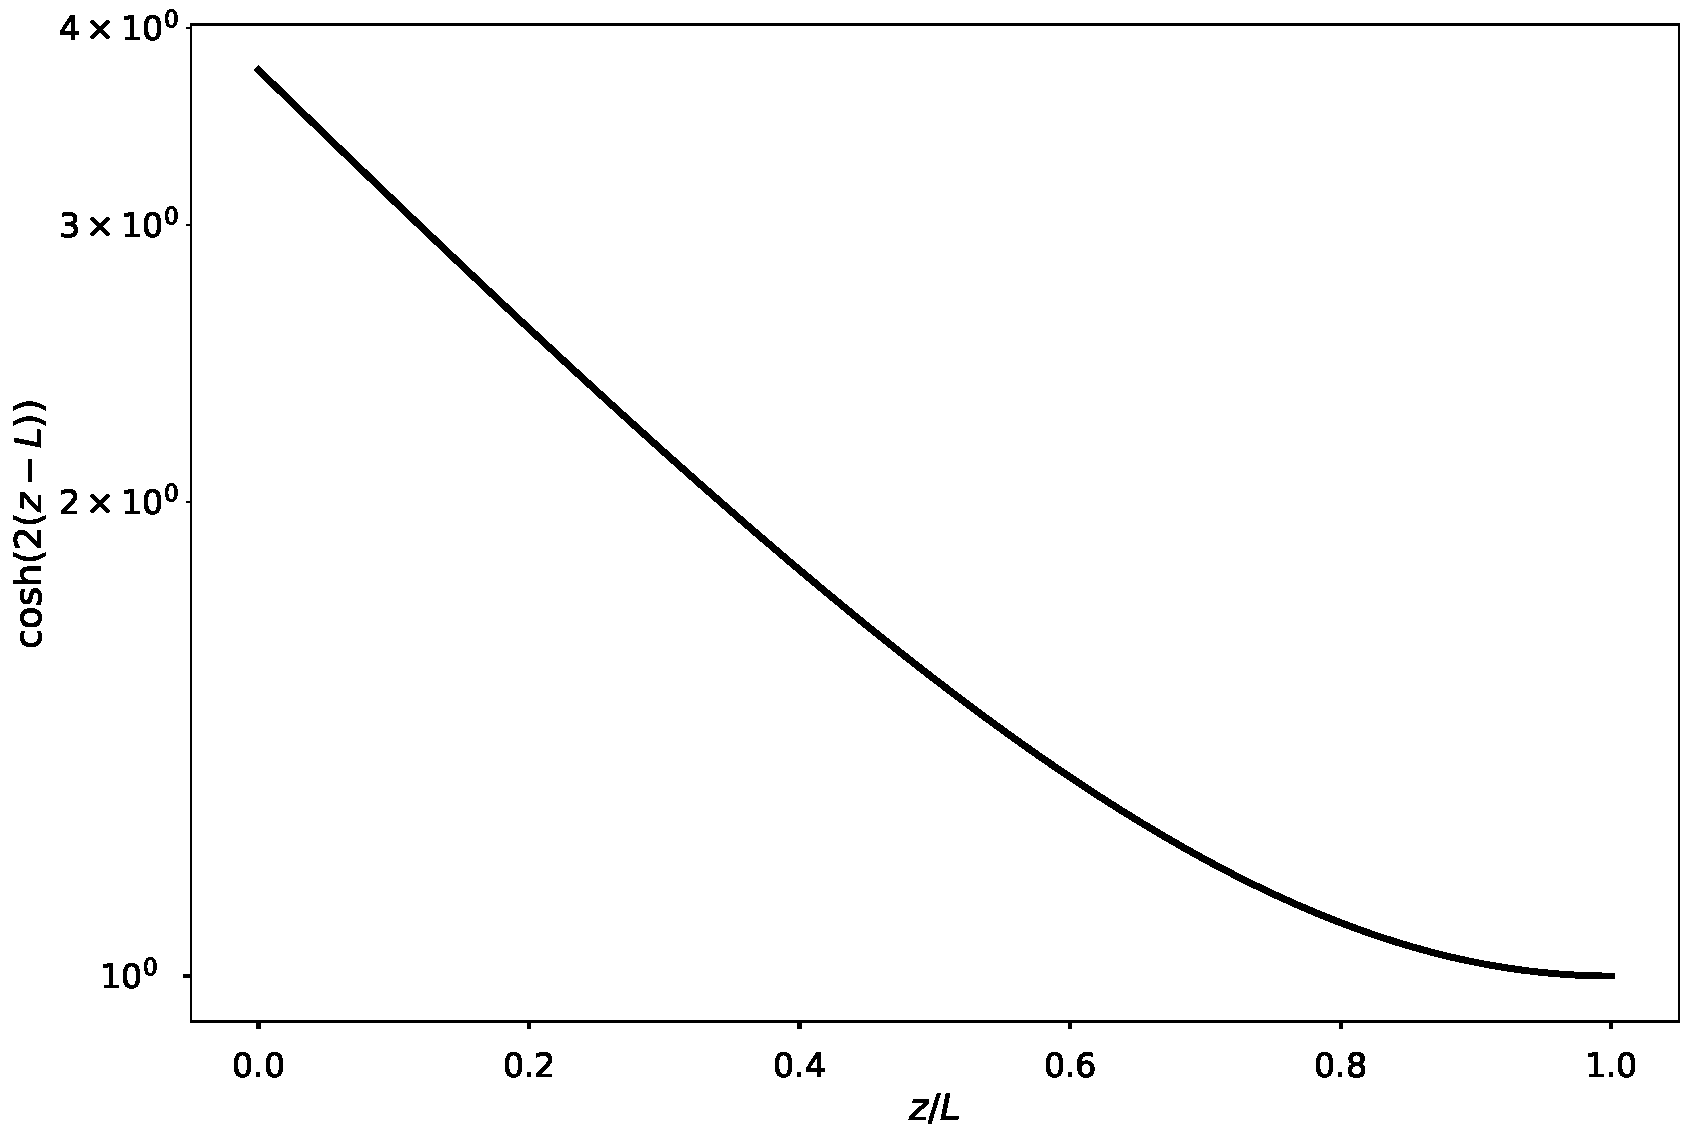
\includegraphics[width=\textwidth]{chapters/assets/halo/cosh.pdf}
    \caption{ An example of $\cosh(2\delta(z-L))$ with $\delta=1$, and $L=5$. This function always reach the minimium at $z=L$.}
    \label{chap:halo-sec:line-sym-fig:cosh}
\end{figure}


We expect the numerical calculations bare the same behavior that the instability leads to no growth but decrease in flavor conversion, assuming the neutrinos start from electron flavor. The result indeed confirms it. Fig.~\ref{chap:halo-sec:line-sym-fig:mu-1.0-reflection-0.07} is an example of it.

\begin{figure}[htbp]
    \centering
    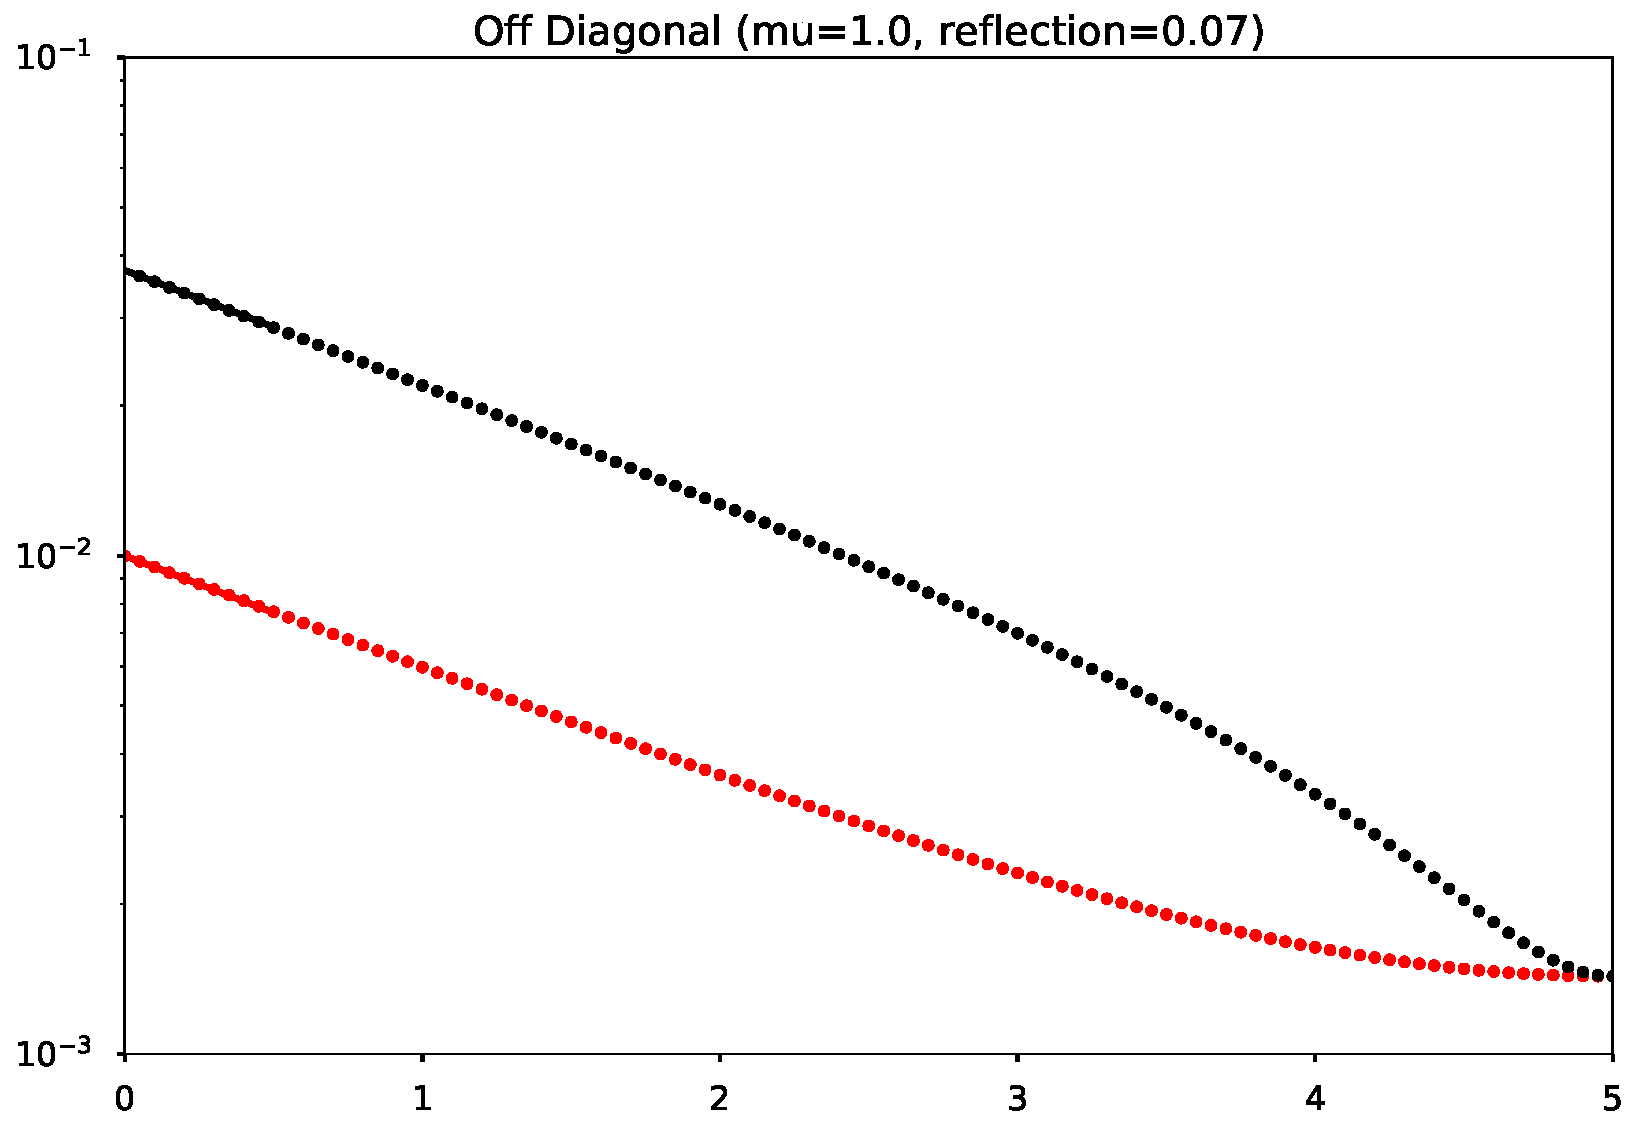
\includegraphics[width=\textwidth]{chapters/assets/halo/mu-1-reflection-0p07.pdf}
    \caption{Absolute value of off diagonal element for $\mu=1.0$, $R=0.07$, $L=5$, with normal hierarchy. The red dots are for the forward beam and the black dots are for the backward beams. The lines are indicating the predictions of linear stability analysis.}
    \label{chap:halo-sec:line-sym-fig:mu-1.0-reflection-0.07}
\end{figure}

For linear stability analysis, I usually identify real characteristic values of the linearized equation of motion. In bipolar model as explained in Sec.~\ref{chap:app-sec:bipolar}, real characteristic values of the equation of motion indicates exponential growth, while it always indicates exponential decrease in this simplified halo problem. 

I expect that only normal hierarchy has an instability region which is trivial since I noticed that the backward beam is acting like antineutrino beams but with different hierarchies.
\begin{align}
 i \partial_t \mathbf s_F &= \mathbf s_F \times (\mathbf {H}_v +R \mu \mathbf s_B) \\
   i\partial_t \mathbf s_B &= \mathbf s_B \times (- \mathbf H_v - \mu \mathbf s_F) .
\end{align}
Compare to Eq.~\ref{chap:app-sec:bipolar-eqn:flavor-isospin-eom}, I notice that 
the reflected beam works as an antineutrino beam but the system becomes the opposite hierarchy compared to bipolar model. I find the instability regions in Fig.~\ref{chap:halo-sec:line-sym-fig:instability-regions}.


\begin{figure}[htbp]
    % \centering
    \minipage{0.49\textwidth}
    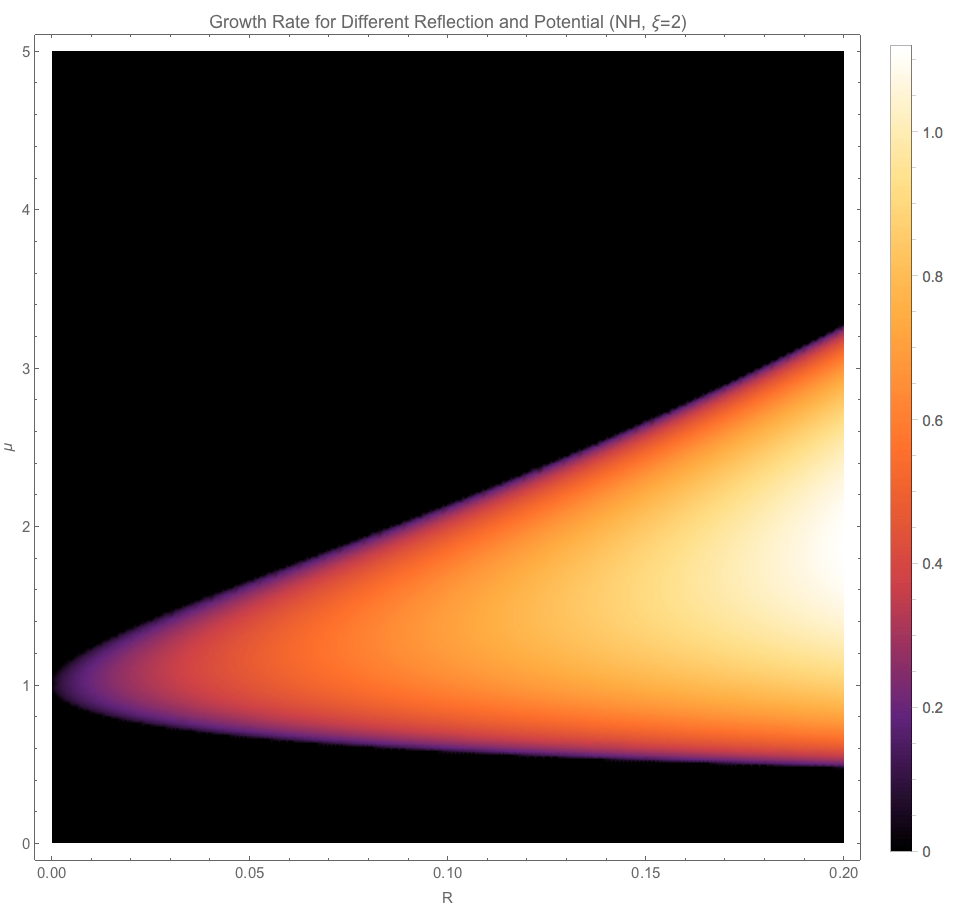
\includegraphics[width=\textwidth]{chapters/assets/halo/growth-rate-mu-refl-nh.jpg}
    \endminipage\hfill
    \minipage{0.49\textwidth}
    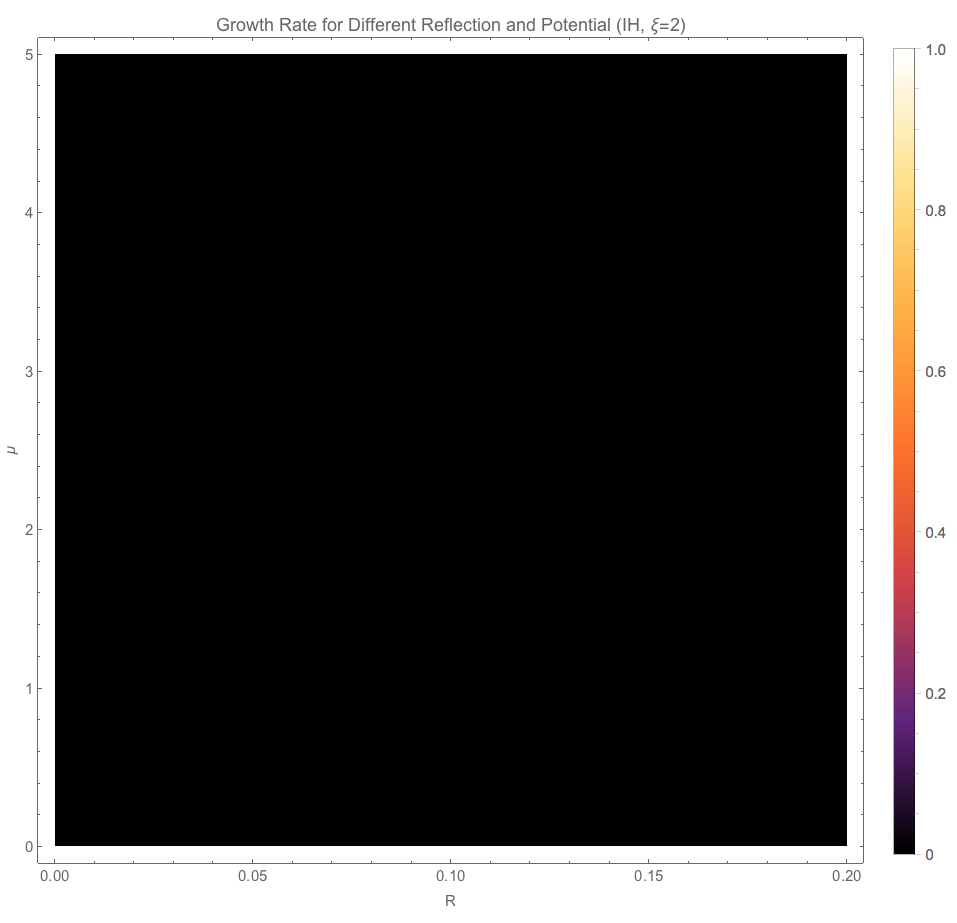
\includegraphics[width=\textwidth]{chapters/assets/halo/growth-rate-mu-refl-ih.jpg}
    \endminipage\hfill
    \caption{Instability regions for normal hierarchy (left) and inverted hierarchy (right) as a function of neutrino potential $\mu$ and reflection coefficient $R$, with vacuum mixing angle set to 0. No instabilities is found in inverted hierarchy.}
    \label{chap:halo-sec:line-sym-fig:instability-regions}
\end{figure}




\subsection{Two Beams Model with Reflection}

The model is naturally extended to a two beams model including both neutrinos and antineutrinos. The configuration is exactly the same as shown in Fig.~\ref{chap:halo-sec:line-fig:line-model}.

As the first step we work out the linear stability analysis. The four equations of motion are
\begin{align}
    i \partial_z \rho_1 = & [ H_1, \rho_1 ], \\
    i \partial_z \rho_2 = & [ H_2, \rho_2 ], \\
    -i \partial_z \rho_3 = & [ H_3, \rho_3 ], \\
    -i \partial_z \rho_4 = & [ H_4, \rho_4 ],
\end{align}
where ${}_1$ and ${}_2$ are the quantities for two forward beams while ${}_3$ and ${}_4$ are the quantities for the corresponding backward going beams. For the purpose of this analysis we set $\theta_v = 0$. The Hamiltonians are
\begin{align}
    H_1 =& -\eta \omega_v \sigma_3 + g_2 \chi_- \mu_2 \rho_2 + g_2 \chi_+ R \mu_2 \rho_4 + g_1 \chi_1 R \mu_1 \rho_3, \\
    H_2 =& \eta \omega_v \sigma_3 + g_1 \chi_- \mu_1 \rho_1 + g_2 \chi_2 R \mu_2 \rho_4 + g_1 \chi_+ R \mu_1 \rho_3, \\
    H_3 =& -\eta \omega_v \sigma_3 + R g_2 \chi_- \mu_2 \rho_4 + g_2 \chi_+\mu_2 \rho_2 + g_1 \chi_1 \mu_1 \rho_1, \\
    H_4 =& \eta \omega_v \sigma_3 + R g_1 \mu_1 \chi_- \rho_3 + g_1 \chi_+ \mu_1 \rho_1 + g_2 \chi_2 \mu_2 \rho_2.
\end{align}

I have defined 
\begin{align*}
    \chi_+ = & 1 - \cos ( \theta_1 + \theta_2 ), \\
    \chi_- = & 1 - \cos ( \theta_1 - \theta_2 ), \\
    \chi_1 = & 1 - \cos ( 2\theta_1 ), \\
    \chi_2 = & 1 - \cos ( 2\theta_2 ),
\end{align*}
and $g_i$ represents the energy spectrum of the neutrinos and $\eta$ stands for the hierarchy.

% Linear stability analysis can be done using computer.

\section{\label{chap:halo-sec:num}Relaxation Method for Neutrino Halo Problem}


We choose a relaxation method scheme to solve this non-local boundary value problem numerically. To begin with, we write down the discretization scheme.
\begin{align}
    \rho(t+\Delta t) &= \left[  \cos( 2 h \Delta t)\rho_n -  2 u_i \rho_i u_n \right]\sigma_n \\
    &= \left[  \cos( 2 h \Delta t) \rho_n +  2 \sin^2(h \Delta t) u'_i \rho_i u'_n \right]\sigma_n
\end{align}
The reason that we use fixed step size for this problem is that it's easier to calculate the neutrino self-interactions on such fixed grids. The algorithm is described as
\begin{enumerate}
    \item
Calculate forward beam using 0 backward beam;
\item
Calculate backward beam and forward beam together using the state of beams from the previous step current counter beams;
\item
Repeat the previous step until the state of the beams reach equilibrium.
\end{enumerate}
To speed up the calculations, I also implemented OpenMP for parallel computing. The code is tested using vacuum oscillations (shown in Fig.~\ref{chap:halo-sec:num-fig:compare-vac-bipolar}) and bipolar models. The reason that we still have conversions is because of the vacuum term, which is additional to linear stability analysis. It is also proven to reach equilibrium quickly as shown in Fig.~\ref{chap:halo-sec:num-fig:relax-color}. 

\begin{figure}[htbp]
    \minipage{\textwidth}
    % 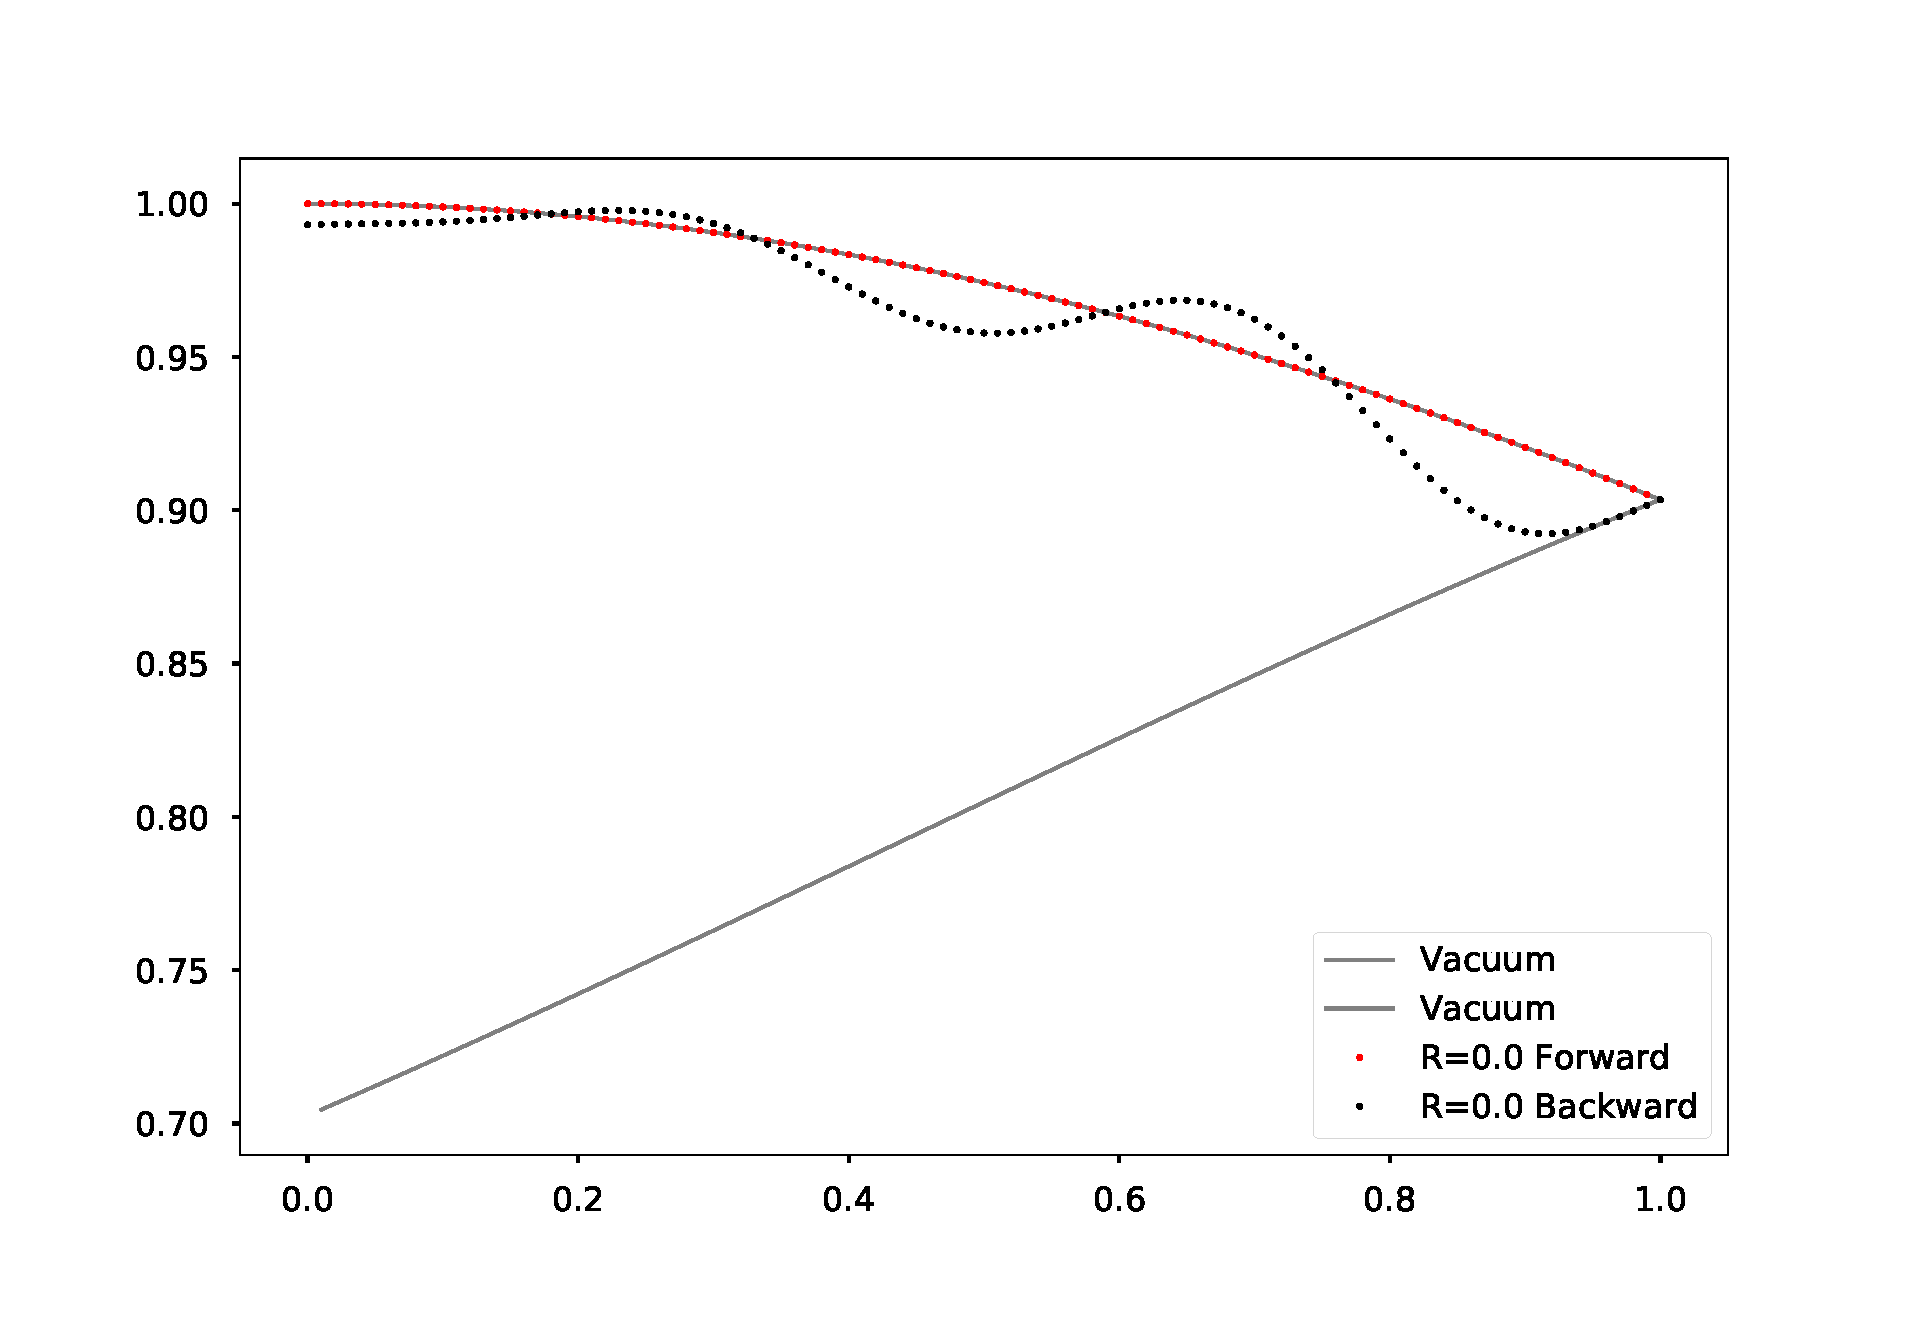
\includegraphics[width=\textwidth]{chapters/assets/halo/halo-mu-4-compare-vac.pdf}
    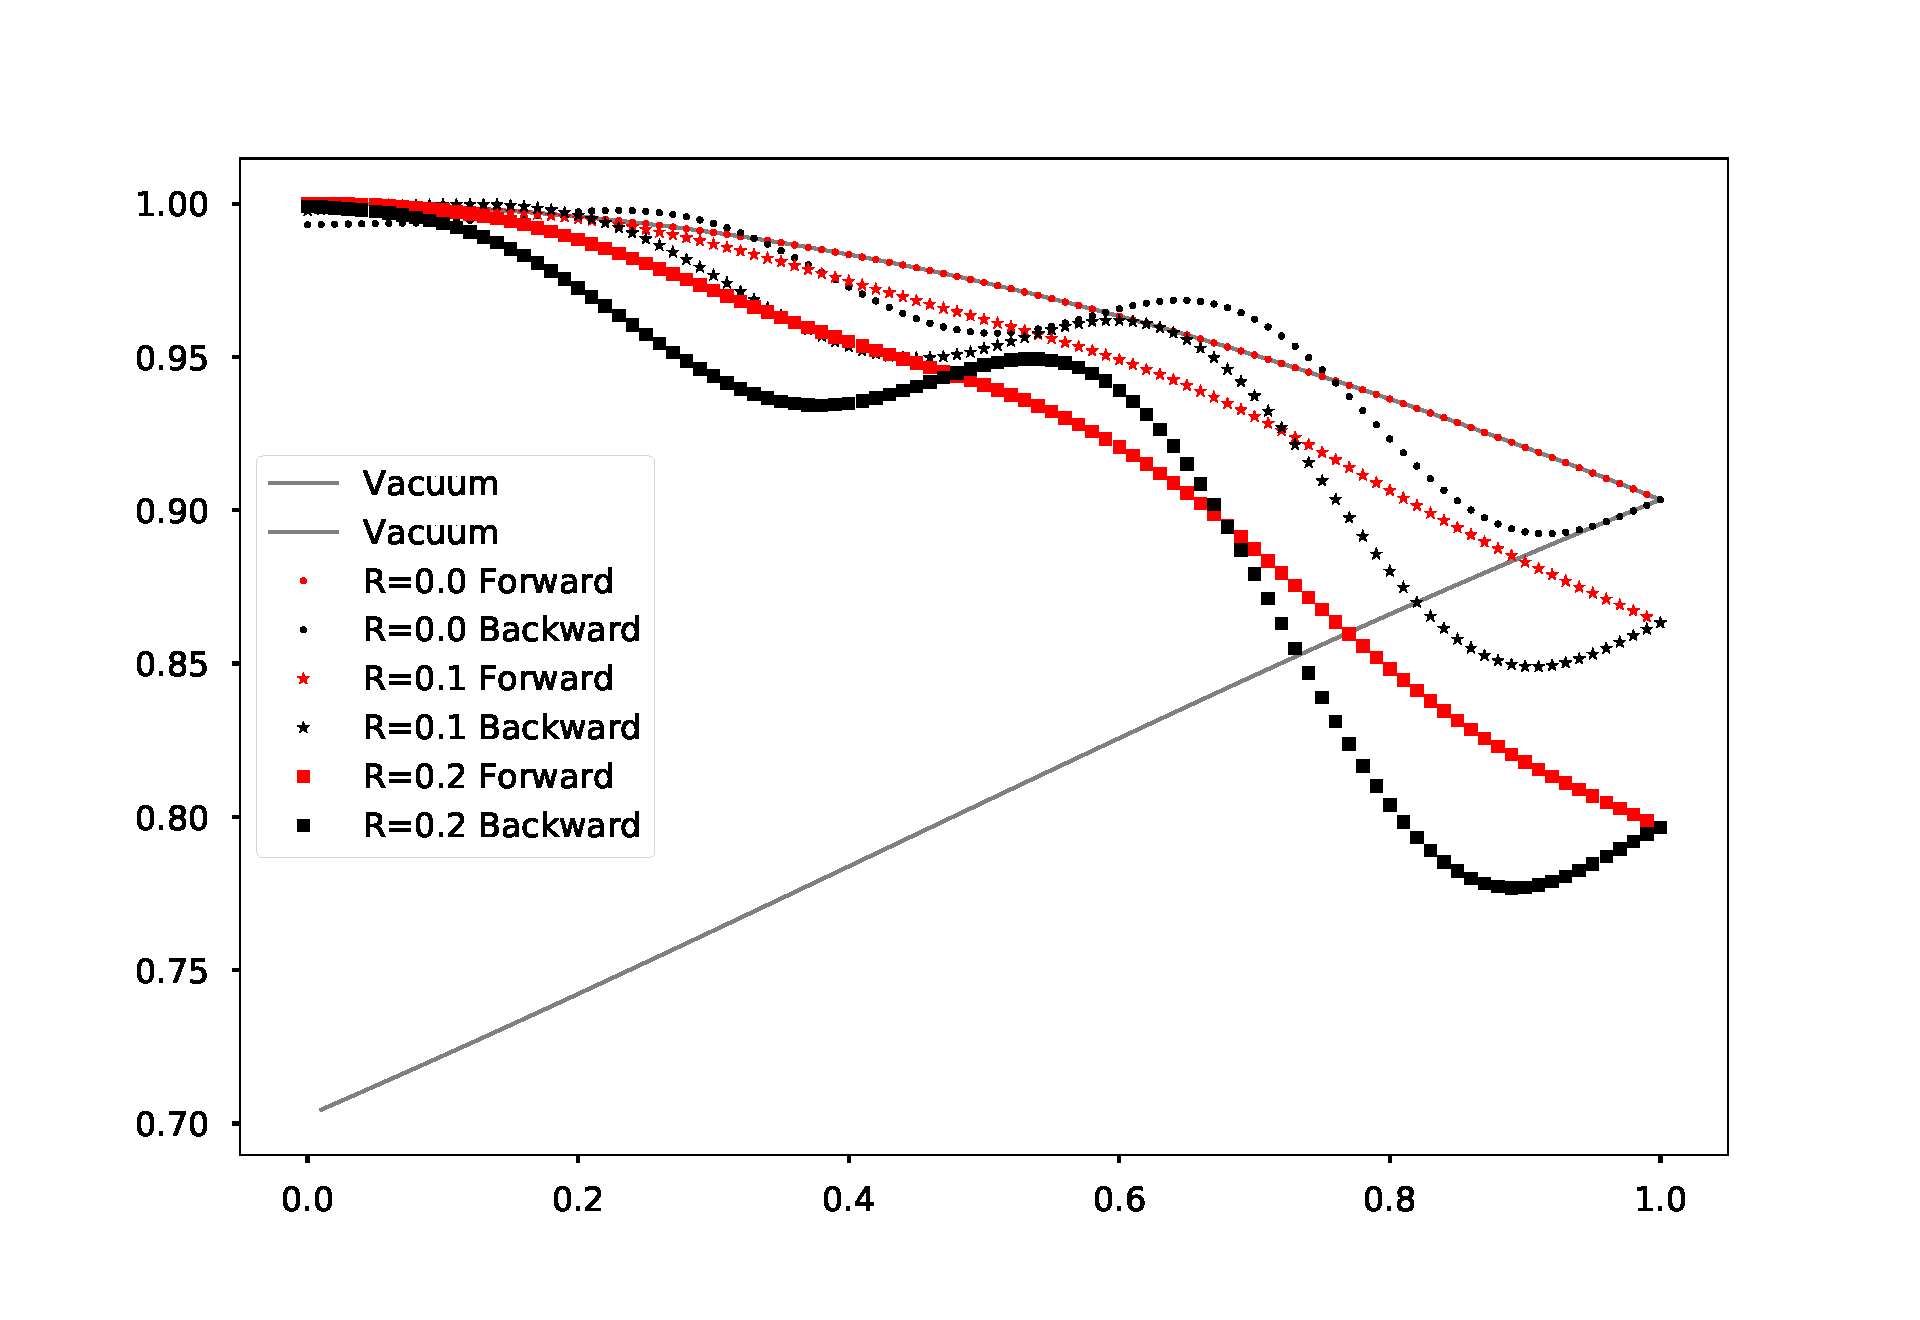
\includegraphics[width=0.49\textwidth]{chapters/assets/halo/halo-mu-4-r-multiple.pdf}
    \endminipage\hfill
    \minipage{\textwidth}
    \includegraphics[width=0.49\textwidth]{chapters/assets/halo/halo-mu-4-compare-bipolar.pdf}
    \endminipage\hfill
    \caption{The left panel validates code by setting reflection to zero and approach vacuum for single forward beam. Meanwhile, we notice that for nonzero reflections, more conversion is done, which makes sense due to the similarity between $R$ and the asymmetry parameter $\alpha$ in bipolar model. The right panel validates the code by setting reflection to zero and compare with bipolar model for two beams case, where the slope is matching the theoretical value $3.85$.}
    \label{chap:halo-sec:num-fig:compare-vac-bipolar}
\end{figure}

\begin{figure}[htbp]
    \centering
    \includegraphics[width=0.8\textwidth]{chapters/assets/halo/relax-color.png}
    \caption{Relaxation method reaches equilibrium after some steps. The horizontal axis is the $z$ direction while the vertical axis is the number of iteration steps. The color indicates the survival probability for electron flavor. This calculation sets $\mu = 4$, $R=0.2$, and is done within range $[0,1]$. Equilibrium is reached around step 400 and the neutrino states stays in equilibrium.}
    \label{chap:halo-sec:num-fig:relax-color}
\end{figure}





%%%%%%%%%%%%%%%%%%%%%%%%%%%%%%%%%%%%%%%%%%%%%%%%%%%%%%%%%%%%%%%%%%%%%%%%%
%%%%%%%%%%%%%%%%%%%%%% Conclusion %%%%%%%%%%%%%%%%%%%%%%%%%%%%
%%%%%%%%%%%%%%%%%%%%%%%%%%%%%%%%%%%%%%%%%%%%%%%%%%%%%%%%%%%%%%%%%%%%%%%%%


\section{\label{chap:collective-sec:conclusion}Conclusion}


The dispersion relations can be extracted from the linearized form of the equation of motion for collective neutrino oscillations. The dispersion relation becomes quadratic for neutrino emission with two zenith angles. Thus two solutions should be found for $\omega$ and $k$. The dispersion relations are hyperbolas and the gaps between the lines corresponds to instabilities. However, this correspondence doesn't hold for neutrinos emitted from more zenith angles. For more realistic spectrum, I have proved that instabilities propagate in regions of either $\omega>0$ or $\omega<0$ and never cross $\omega=0$. Hence the dispersion relation gaps should be defined as gaps between the dispersion relation curves and the axis $\omega=0$ instead of the dispersion relation curves. I have also showed that instabilities is not necessarily shown as gap in dispersion relations for neutrino emission with more than two zenith angles and box spectrum with crossing. Through the discussions, I demonstrated that the relation between dispersion relation gaps and instabilities should be used with caution.


The second problem discussed in this chapter is the halo problem, which brings in more complexities to the neutrino oscillations. In the spirit of numerical methods, I developed a parallelable relaxation method, using C++ and OpenMP. Both the analytical and numerical results showed that for the two realms, either single forward beam or two forward beams, the results are compared with bipolar model. This simple model is very similar to the bipolar model thus I can perform linear stability analysis and verify my numerical method. The reflection indeed may enhance the flavor conversions but it is not a new type of instability. Future work should be done to explore the effect of symmetry breaking and multiple emission beams.

% %!TEX root = ../dissertation.tex


\chapter{\label{chap:halo}Neutrino Halo Problem}


One of the big questions about neutrino oscillations in supernovae is the so called halo problem. Cherry et al showed that neutrino flavor conversions are greatly affected by the back scattered neutrinos in supernovae~\cite{Cherry2012}. Neutrinos around supernovae are scattered and some of them are scattered to move almost backward. On the other hand, neutrino self-interactions is proportional to the inner product of momenta of neutrinos, which leads to the dependence on $1-\cos\theta$ where $\theta$ is the angles between momenta of two neutrinos. Most of the research has been concentrating on mostly forward scattering, with small values for $1-\cos\theta$. For back ward scattered neutrinos, the interaction potential can be much larger than the forward scattered neutrino contributions. Though the work by Sarikas et al showed that matter suppression is still significant within this region~\cite{Sarikas2012a}, it is not clear how exactly the neutrino halo alters neutrino oscillations. The halo problem itself is worth more calculations.


\section{\label{chap:halo-sec:line}Line Model}

We continue to use the simplified line model and build our intuitions out of it. The halo problem is simplified to have neutrinos emitted from a line $z=0$ homogeneously, which are reflected from a certain distance $z=L$. In principle, the reflection angles doesn’t have to be Snell’s law. The scattering can be in any angle with different amplitudes. Here I am using this very simple Snell’s law just to explore the effect of halo. It's crucial to keep an eye on the simplifications in this line model.
\begin{itemize}
    \item Neutrinos are emitted from a line, which is not the case in a real supernova.
    \item Neutrinos are emitted with translation symmetry on the line. Breaking the symmetry might bring in other qualitatively different results.
    \item Neutrinos are reflected from a certain surface $z=L$, which is different from reality where neutrinos are scattered everywhere.
    \item Neutrinos are reflected according to Snell's law.
    \item Neutrinos are homogeneously reflected at $z=L$.
\end{itemize}



\begin{figure}
    \centering
    \includegraphics[width=\textwidth]{chapters/assets/halo/line-model.pdf}
    \caption{Line model used for halo problem. Neutrinos are emitted from the bottom line and reflected at the top line.}
    \label{chap:halo-sec:line-fig:line-model}
\end{figure}


The algorithm that I used is relaxation method. The algorithm is meant to find the equilibrium state of neutrino oscillations with the presence of halo.
\begin{enumerate}
\item Calculate forward beam using 0 backward beam;
\item Calculate backward beam using forward beam calculated in 1;
\item Calculate forward beam using backward beam calculated in 2;
\item Repeat until the beams reach equilibrium.
\end{enumerate}


\section{\label{chap:halo-sec:line-sym}Neutrino Beams Only}

As a first step, I calculated neutrino oscillations with only neutrino beams. Before we rush to the numerical results, I linearized the equation of motion and worked out the linear stability analysis.

In linear regime, we define the density matrices for forward and backward beams to be
\begin{align*}
   \rho_F &= \frac{1}{2} \begin{pmatrix}
   1 & \epsilon_F \\
   \epsilon_B^* & -1
   \end{pmatrix} \\
   \rho_B &= \frac{1}{2} \begin{pmatrix}
   1 & \epsilon_B \\
   \epsilon_B^* & -1
   \end{pmatrix}.
\end{align*}
The Hamiltonian for forward and back ward beams are
\begin{align*}
   H_F &= H_v + \mu \rho_F \\
   H_B &= H_v + R \mu \rho_B.
\end{align*}
We will investigate the instability for zero mixing angle for new instabilities. The linearized equation of motion can be simplified to
\begin{align*}
   i\partial_z \begin{pmatrix}
   \epsilon_F \\
   \epsilon_B
   \end{pmatrix} = \begin{pmatrix}
   -\omega_v + R \xi \mu & - R \xi \mu \\
   \xi \mu & \omega_v - \xi \mu
   \end{pmatrix} \begin{pmatrix}
   \epsilon_F \\
   \epsilon_B
   \end{pmatrix}.
\end{align*}
This equation can be easily solved. The eigenvalues are
\begin{align*}
   \Omega_+ &= \frac{1}{2} ( (R-1)\xi\mu + \sqrt{\Delta} ) \\
   \Omega_- &= \frac{1}{2} ( (R-1)\xi\mu - \sqrt{\Delta} ),
\end{align*}
where
\begin{equation}
   \Delta = (1-R)^2 \mu^2 \xi^2 - 4\mu\xi \omega_v (1+R) + 4\omega_v^2.
\end{equation}
The corresponding eigenvectors are
\begin{align*}
   V_+ &=\begin{pmatrix}
   \frac{ -2\omega_v + \xi \mu (1+R) + \sqrt{\Delta} }{2\xi\mu} \\
   1
   \end{pmatrix} \\
   V_- &=\begin{pmatrix}
   \frac{ -2\omega_v + \xi \mu (1+R) - \sqrt{\Delta} }{2\xi\mu} \\
   1
   \end{pmatrix}.
\end{align*}
The general solution to the equation is
\begin{equation*}
   \begin{pmatrix}
   \epsilon_F(z) \\
   \epsilon_B(z)
   \end{pmatrix} = C_+ V_+ e^{-i \Omega_+ z} +  C_- V_- e^{-i \Omega_- z}.
\end{equation*}

The special property about this reflection problem is that the density matrices for the forward and backward beams should be the same at the reflection point, say $z=L$. With such a simple relation, we can find the relations between $C_\pm$ by setting $\epsilon_F(L)=\epsilon_B(L)$,
\begin{equation}
   \frac{C_+}{C_-} = e^{-i(\Omega_- -\Omega_+)L} \frac{ \sqrt{\Delta} +  2\omega_v + \mu \xi (1-R) }{\sqrt{\Delta} -  2\omega_v - \mu \xi (1-R)}.
\end{equation}
The solution to be problem can be simplified,
\begin{equation}
   \begin{pmatrix}
   \epsilon_F(z) \\
   \epsilon_B(z)
   \end{pmatrix} = C_- e^{-i\Omega_- L} \left( \frac{ \sqrt{\Delta} +  2\omega_v + \mu \xi (1-R) }{\sqrt{\Delta} -  2\omega_v - \mu \xi (1-R)} V_+ e^{-i \Omega_+ (z-L)} +  V_- e^{-i \Omega_- (z-L)} \right).
\end{equation}

We are interested in the absolute values of each elements so that the overall factors can be neglected. The forward beam evolution is obtained by taking the absolute value of $\epsilon_F$,
\begin{align*}
   \left\vert \epsilon_F \right\vert \propto & \lvert (2\omega_v +\xi\mu(1-R) +i \delta ) ( -2\omega_v + \xi\mu(1+R) + i \delta ) e^{\delta(z-L)} \\ 
   &+ ( -2\omega_v - \xi\mu(1-R) +i \delta ) ( -2\omega_v + \xi\mu(1+R) - i \delta ) e^{-\delta(z-L)} \rvert,
\end{align*}
in which $\sqrt{\Delta}$ is replaced by $i \delta$. We collecting terms and verify that it has the form
\begin{equation}
   \left\vert \epsilon_F \right\vert \propto A + B \cosh( 2\delta(L-z) ),
\end{equation}
where $B\leq 0$.
The only $z$ dependent term is $\cosh( 2\delta(L-z) )$, which is decreasing within $[0,L]$ and is increasing in $[L,2L]$. The slope at $z=L$ is 0. An example is plotted in Fig.~\ref{chap:halo-sec:line-sym-fig:cosh}.


\begin{figure}
    \centering
    \includegraphics[width=\textwidth]{chapters/assets/halo/cosh.pdf}
    \caption{ An example of $\cosh(2\delta(z-L))$ with $\delta=1$, and $L=5$.}
    \label{chap:halo-sec:line-sym-fig:cosh}
\end{figure}


We expect the numerical calculations bare the same behavior that the instability leads to no growth but decrease in flavor conversion, assuming the neutrinos start from electron flavor. The result indeed confirms it. Fig.~\ref{chap:halo-sec:line-sym-fig:mu-1.0-reflection-0.07} is an example of it.

\begin{figure}[htbp]
    \centering
    \includegraphics[width=\textwidth]{chapters/assets/halo/mu-1-reflection-0p07.pdf}
    \caption{Absolute value of off diagonal element for $\mu=1.0$, $R=0.07$, $L=5$. The red dots are for the forward beam and the black dots are for the backward beams. The lines are indicating the predictions of linear stability analysis.}
    \label{chap:halo-sec:line-sym-fig:mu-1.0-reflection-0.07}
\end{figure}

For linear stability analysis, we usually identify real characteristic values of the linearized equation of motion. In bipolar model as explained in Sec.~\ref{chap:app-sec:bipolar}, real characteristic values of the equation of motion indicates exponential growth, while it always indicates exponential decrease in this simplified halo problem.

\section{Conclusion}

Halo problem brings in more parameters to neutrino oscillations.
%!TEX root = ../dissertation.tex
\chapter{Conclusion}
\label{conclusion}

We conclude that neutrinos oscillate.
% %!TEX root = ../phd-thesis-lei-ma.tex

%%%%%%%%%%%%%%%%%%%%%%%%%%%%%%%%%%%%%%%%%%
%%%%%%%%%%%%% APPENDIX  %%%%%%%%%%%%%%%%%%
%%%%%%%%%%%%%%%%%%%%%%%%%%%%%%%%%%%%%%%%%%


\part*{Appendices}
\label{chap:appendices}
\addcontentsline{toc}{chapter}{Appendices}
 % Next lines duplicated from .toc file and used to create mini
 % "Appendix Table of Contents," if desired:
   \contentsline {chapter}{\numberline {A} Conventions}{}
   \contentsline {chapter}{\numberline {B} Rabi Oscillations}{}
   \contentsline {chapter}{\numberline {C} MSW Effect Revisited}{}
%   \contentsline {chapter}{\numberline {B}Derivation of $A = \pi r^2$}{5}
 % End mini table of contents

\appendix



\chapter{\label{chap:app-sec:conventions}Conventions}

\section{\label{chap:app-sec:conventions-subsec:terms}Terms}

\begin{itemize}
    \item 
    Normal hierarchy for two flavors is always defined as $m_2^2-m_1^2>0$.
    \item
    Solar neutrino mass splitting is $\delta m_{12}$, while atmospheric neutrino mass splitting refers to $\delta m_{23}$.
\end{itemize}





\section{\label{chap:app-sec:conventions-subsec:units}Units}


Natural units system makes the calculations of neutrinos convenient. By definition, we set reduced Planck constant and speed of light to be 1, $\hbar = 1 = c$.
The conversion between natural units and SI can be down by using the following relations,
\begin{align}
   1 \mathrm{GeV} &= 5.08 \times 10^{15} \mathrm {m^{-1}} \\
   1 \mathrm{GeV} &= 1.8\times 10^{-27} \mathrm{kg}
\end{align}
To convert between different physical quantities in this thesis, I always use the following tips.
\begin{itemize}
    \item The energy-mass-momentum relations becomes $E^2 = p^2 + m^2c^2 = p^2 + m^2$. Thus mass $m$, momentum $\mathbf p$ and energy $E$ have the same dimension.
    \item An example of angular momentum in quantum mechanics is $L_z = m\hbar = m$ where $m$ is a quantum number. $\hbar$ is of dimension angular momentum.
    \item A plane wave in quantum mechanics is $\Psi = A e^{ \frac{E t - p x}{\hbar} }$. $\frac{E t - p x}{\hbar}$ should be dimensionless, which means $px$ has dimension angular momentum, which is obvious, meanwhile we notice that $E t$ also has the dimension of angular momentum. Previously we noticed momentum has the same dimension with energy, we should have time $t$ with the same dimension of length $x$. Also we can conclude that length and time have the same dimenson as $1/E$.
\end{itemize}



\section{Pauli Matrices and Rotations}


Given a rotation
\begin{equation}
   U = \begin{pmatrix} \cos \theta & \sin \theta \\ -\sin\theta & \cos \theta \end{pmatrix}, 
\end{equation}
its effect on Pauli matrices are
\begin{align}
      U^\dagger \sigma_3 U  &=\cos 2\theta \sigma_3 + \sin 2\theta \sigma_1 \\
  U^\dagger \sigma_1 U & = -\sin 2\theta \sigma_3 + \cos 2\theta \sigma_1.
\end{align}



\section{Useful Conversions in Neutrino Physics}

Using natural units, length = time = 1/energy, we could rescale almost all quantities in neutrino oscillations using energy, or whatever characteristic scale we have.

We use two flavor vacuum oscillations between the two masses $m_1$ and $m_2$ as an example. The characteristic energy scale is the oscillation frequency $\omega_{v,21}$. The equation of motion
\begin{align}
   i\frac{d}{d x} \Psi = \frac{\omega_v}{2}(-\cos 2\theta_v \boldsymbol{\sigma_3} + \sin 2\theta_v \boldsymbol{\sigma_1}) \Psi,
\end{align}
can be rescaled using the characteristic energy scale $\omega_{v,21}$
\begin{align}
   i\frac{d}{d \hat x} \Psi = \frac{1}{2}(-\cos 2\theta_v \boldsymbol{\sigma_3} + \sin 2\theta_v \boldsymbol{\sigma_1})\Psi ,
\end{align}
where $\hat x = \omega_{v,21} x$. It is convenient for numerical calculations to convert quantities into dimensionless ones.

However, we usually discuss oscillation length in SI units for a grip of the picture. To convert from natural units to SI units, we write down the conversion here. The oscillation angular frequency is given by
\begin{align}
   \omega_{v,21} &= \frac{\delta m^2}{2E} \nonumber\\
   &=  \left(\frac{7.5\times 10^{-5}\mathrm{eV}^2}{2\times 1\mathrm{MeV}} \right) \left(\frac{\delta m^2}{7.5\times 10^{-5}\mathrm{eV}^2} \right) \frac{1\mathrm{MeV}}{E} \nonumber\\
   &= 3.75\times 10^{-11}\mathrm{eV}  \left(\frac{\delta m^2}{7.5\times 10^{-5}\mathrm{eV}^2}\right) \left(\frac{1\mathrm{MeV}}{E}\right) .
\end{align}
On the other hand, electro-volt is related to length through the useful formula
\begin{equation}
   197\mathrm{MeV}\cdot \mathrm{fm} = \hbar c = 1.
\end{equation}
Thus we have the oscillation angular frequency written as
\begin{align}
   \omega_{v,21} &= 3.75\times 10^{-11}\mathrm{eV}  \frac{\delta m^2}{7.5\times 10^{-5}\mathrm{eV}^2} \frac{1\mathrm{MeV}}{E} \nonumber\\
   &= 3.75\times 10^{-17}\mathrm{MeV}  \frac{\delta m^2}{7.5\times 10^{-5}\mathrm{eV}^2} \frac{1\mathrm{MeV}}{E}\nonumber \\
   &= 1.90\times 10^{-4}  \mathrm{m}^{-1}  \frac{\delta m^2}{7.5\times 10^{-5}\mathrm{eV}^2} \frac{1\mathrm{MeV}}{E}.
   \label{common-sense-eqn-omega-v-si-unit}
\end{align}
Similarly for $\delta m_{32}=2.4\times 10^{-3}\mathrm{eV^2}$ the frequency is
\begin{align}
   \omega_{v,32} =\frac{\delta m^2_{32}}{2E} = 6.3\times 10^{-3} \mathrm{m}^{-1}  \frac{\delta m^2_{32}}{2.5\times 10^{-3} \mathrm{eV}^2 } \frac{1MeV}{E}.
\end{align}
With the results for angular frequencies, the rescaled length $\hat x$ is restored using
\begin{align}
    x = \frac{\hat x}{\omega_v} &= \frac{\hat x}{  1.90\times 10^{-4}  \mathrm{m}^{-1}  \frac{\delta m^2}{7.5\times 10^{-5}\mathrm{eV}^2} \frac{1\mathrm{MeV}}{E} } \\
    &= \frac{\hat x}{0.190} \mathrm{km} \frac{7.5\times 10^{-5}\mathrm{eV}^2}{\delta m^2}  \frac{E}{1\mathrm{MeV}}.
\end{align}


Another important example is the 2 flavor neutrino oscillations in constant matter background potential $\lambda_c = \sqrt{2}G_{\mathrm F} n_e$. The characteristic energy scale is $\omega_m$ which is calculated using
\begin{equation}
   \omega_m = \omega_v \sqrt{ \frac{\lambda_c}{\omega_v}^2 + 1 - 2 \frac{\lambda_c}{\omega_v}\cos 2\theta_v }.
   \label{common-sense-eqn-omega-m}
\end{equation}
Meanwhile, the effective mixing angle $\theta_m$ is determined by
\begin{equation}
   \tan 2\theta_m = \frac{\sin 2\theta_v}{\cos 2\theta_v - \frac{\lambda}{\omega_v} }.
\end{equation}
Similar to vacuum equation of motion, we rescale the equation of motion in constant background using $\omega_m$
\begin{equation}
   i \frac{d}{d\hat x} \Psi = \frac{1}{2}(-\cos 2\theta_m \boldsymbol{\sigma_3} + \sin 2\theta_m \boldsymbol{\sigma_1})\Psi ,
\end{equation}
we find out the scaled distance
\begin{equation}
   \hat x = \omega_m x.
\end{equation}
To reverse the process and find out the actual SI unit distance after the numerical calculation, we use
\begin{equation}
   x = \frac{\hat x}{\omega_m}.
   \label{common-sense-eqn-actual-distance-constant-matter}
\end{equation}
The procedure will be the following.
\begin{itemize}
    \item Calculate $\omega_v$ using Eq.~\ref{common-sense-eqn-omega-v-si-unit}.
\item Calculate $\hat\lambda_c = \frac{\lambda_c}{\omega_v}$.
\item Calculate $\omega_m$ using Eq.~\ref{common-sense-eqn-omega-m}.
\item Find out the actual distance using Eq.~ \ref{common-sense-eqn-actual-distance-constant-matter}.
\end{itemize}


\chapter{\label{app:rabi-oscillations}Rabi Oscillations}

%  trim={<left> <lower> <right> <upper>}
%\begin{widetext}
% \begin{figure*}
%     \centering
%     \begin{subfigure}[b]{0.5\textwidth}
%         \centering
%         \includegraphics[trim={2cm 3.2cm 9.5cm 1cm},clip]{chapters/assets/rabi/rabi-isospin-static-frame}
%     \caption{}
%     \label{fig-rabi-isospin-static-frame}
%     \end{subfigure}%
%     ~
%     \begin{subfigure}[b]{0.5\textwidth}
%         \centering
%         \includegraphics[trim={6cm 3cm 9.5cm 2cm},clip]{chapters/assets/rabi/rabi-isospin-rotating-frame}
%         \caption{}
%         \label{fig-rabi-isospin-rotating-frame}
%     \end{subfigure}
%     \caption{Rabi oscillations in static frame and rotating frame. In both figures the red dashed vector is the flavor isospin, while the black solid vectors are the vectors of Hamiltonian. The left panel shows the rotating Hamiltonian $\mathbf{H}_3+\mathbf{H}_+$. The right panel shows the rotation of flavor isospin around a static vector $\mathbf{H}'_3+\mathbf{H}'_+$ in the rotating frame.}
%     \label{fig-rabi-isospin-different-frame}
% \end{figure*}
%\end{widetext}

\begin{figure}
        \centering
        \includegraphics[width=\columnwidth, trim={20cm 10cm 50cm 10cm},clip]{chapters/assets/rabi/rabi-isospin-rotating-frame}
    \caption{Rabi oscillations in corotating frame. The red dashed vector is the flavor isospin, while the black solid vectors are the vectors of Hamiltonian. The flavor isospin vector is precessing around vector of total Hamiltonian $\mathbf{H}_3+\mathbf{H}_+$.}
    \label{fig-rabi-isospin-rotating-frame}
\end{figure}

In this appendix we introduce flavor isospin \cite{Duan2006a} to Rabi oscillations and derive the transition probabilities as well as explain the resonance and width briefly.


The Hamiltonian for Rabi oscillation is
\begin{equation}
    H_{\mathrm R} = -\frac{\omega_{\mathrm R}}{2}\sigma_3 - \frac{A_{\mathrm{R}} }{2}  \left( \cos(k_{\mathrm{R}} t +\phi_{\mathrm{R}})\sigma_1  - \sin(k_{\mathrm{R}} t +\phi_{\mathrm{R}}) \sigma_2\right),
    \label{rabi-oscillation-single-perturbation}
\end{equation}
in which $\omega_{\mathrm R}$ serves as the energy split of the two level system, while $A_{\mathrm{R}}$ and $k_{\mathrm{R}}$ are the strength and frequency of the driving field, respectively. A decomposition of the second term shows that
\begin{equation*}
H_{\mathrm R}
= - \frac{\boldsymbol{\sigma}}{2} \cdot (\mathbf{H}_3 + \mathbf{H}_+ ) ,
\end{equation*}
where $\boldsymbol{\sigma}$ is the the vector of Pauli matrices, and the three vectors are
\begin{align}
    \mathbf{H}_3 = & \begin{pmatrix}
    0 \\ 0 \\ \omega_{\mathrm R}
    \end{pmatrix}, \\
    \mathbf{H}_+ = & \begin{pmatrix}
    A_{\mathrm{R}} \cos(k_{\mathrm{R}} t +\phi_{\mathrm{R}}) \\
    - A_{\mathrm{R}} \sin(k_{\mathrm{R}} t +\phi_{\mathrm{R}}) \\
    0
    \end{pmatrix}.
\end{align}

The three vectors are mapped onto a Cartesian coordinate system, so that $\mathbf{H}_3$ is the vector aligned with the third axis, $\mathbf{H}_+$ is a rotating vectors in a plane perpendicular to $\mathbf{H}_3$. The wave function $\Psi=(\psi_1,\psi_2)^{\mathrm{T}}$ is also used to define the state vector $\mathbf{s}$
\begin{align}
    \mathbf{s} =& \Psi^\dagger \frac{\boldsymbol{\sigma}}{2}\Psi \\
    =& \frac{1}{2}\begin{pmatrix}
    2\,\mathrm{Re}\,(\psi_1^* \psi_2) \\
    2\,\mathrm{Im}\,(\psi_1^*\psi_2) \\
    \lvert \psi_1 \rvert^2 - \lvert \psi_2 \rvert^2
    \end{pmatrix}
\end{align}
The third component of $\mathbf{s}$, which is denoted as $s_3$, is within range $[-1/2,1/2]$. The two limits, $s_3=-1/2$ and $s_3=1/2$ stand for the system in high energy state and low energy state respectively. $s_3=0$ if the system has equal probabilities to be on high energy state and low energy state. The Schr\"odinger equation becomes
\begin{equation}
\frac{\mathrm{d}}{\mathrm{d} t } \mathbf{s} = \mathbf{s} \times \mathbf{H},
\end{equation}
which is the precession equation. For static $\mathbf{H}$, the state vector $\mathbf{s}$ precess around $\mathbf{H}$.

In a frame that corotates with $\mathbf{H}_+$, which is described in Fig.~\ref{fig-rabi-isospin-rotating-frame}, the new Hamiltonian is
\begin{equation}
\frac{\mathrm d}{\mathrm d t } \mathbf{s} = \mathbf{s} \times (\mathbf{H}'_3 + \mathbf{H}‘_+),
\end{equation}
where
\begin{equation}
\mathbf{H}'_3 = \begin{pmatrix}
    0 \\ 0 \\  \omega_{\mathrm{R}} - k_{\mathrm R}
    \end{pmatrix}, \qquad \mathbf{H}'_+ = \begin{pmatrix}
    A_{\mathrm{R}} \\ 0 \\  0
    \end{pmatrix}.
\end{equation}
The state vector $\mathbf{s}$ precess around a static vector $\mathbf{H}'_3 + \mathbf{H}'_+$ with a frequency $\Omega_{\mathrm R} = \sqrt{ \lvert A_{\mathrm{R}}\rvert^2 + (k_{\mathrm{R}} - \omega_{\mathrm R})^2 }$. A geometric analysis by projecting the state vector $\mathbf{s}$ on to the verticle axis shows that
\begin{equation}
s_3 = \frac{1}{2} - \frac{\lvert A_{\mathrm R}\rvert ^2}{\Omega_{\mathrm R}^2}\sin^2\left(\frac{\Omega_{\mathrm R}}{2} t\right).
\end{equation}
Resonance occurs when the term $\mathbf{H}_3$ disappears in this corotating frame, since the state vector $\mathbf{s}$ converts completely between $+1/2$ (low energy state) and $-1/2$ (high energy state).



Such a system has analytical transition probability from low energy state to high energy state
\begin{equation}
    P(t) = \frac{1}{2}(1- 2 s_3(t))= \frac{\left \lvert A_{\mathrm{R}} \right \rvert ^2}{ \Omega_{\mathrm R}^2 } \sin^2 \left( \frac{\Omega_{\mathrm R}}{2} t \right),
    \label{rabi-system-transition-probability}
\end{equation}
where
\begin{equation}
\Omega_{\mathrm R} = \sqrt{ \lvert A_{\mathrm{R}}\rvert^2 + (k_{\mathrm{R}} - \omega_{\mathrm R})^2 }
\end{equation} is known as Rabi frequency. The detuning, which is defined by $k_{\mathrm{R}} - \omega_{\mathrm R}$, determines how off-resonance the system is, and amplitude of driving field $A_{\mathrm{R}}$ determines the resonance width,
\begin{align}
\text{Detuning} =&~\lvert k_{\mathrm{R}} - \omega_{\mathrm R} \rvert, \\
\text{Resonance Width} =&~\lvert A_{\mathrm R} \rvert.
\end{align}
The transition probability oscillates with frequency $\Omega_{\mathrm R}$. However, the amplitude $A_1$ is the dominate factor for oscillation frequency when the system is close to resonance. The phase of the matter potential $\phi_{\mathrm{R}}$ has no effect on the transition probability since it only determines the initial phase of driving Hamiltonian vector $\mathbf{H}_+$. We also notice that the transition amplitude is determined by relative detuning $\RD$, which is defined as
\begin{equation}
    \RD = \left\lvert \frac{ k_{\mathrm R} - \omega_{\mathrm R}}{A_{\mathrm R}} \right\rvert.
\end{equation}


Given a Rabi oscillation system with two driving frequencies
\begin{align*}
    H_{\mathrm R} =& -\frac{\omega_{\mathrm R}}{2}\sigma_3 - \frac{A_{1} }{2}  \left( \cos(k_{1} t +\phi_{1})\sigma_1  - \sin(k_{1} t +\phi_{1}) \sigma_2\right) \nonumber\\
    & - \frac{A_{2} }{2}  \left( \cos(k_{2} t +\phi_{2})\sigma_1  - \sin(k_{2} t +\phi_{2}) \sigma_2\right)
\end{align*}
we decompose it into $\mathbf{H}_{\mathrm R}=\mathbf{H}_3 + \mathbf{H}_{1} + \mathbf{H}_2$, where
\begin{equation*}
    \mathbf{H}_1 =  \begin{pmatrix}
     A_{1} \cos(k_{1}t+\phi_{1}) \\
     A_{1} \sin(k_{1}t+\phi_{1})  \\
     0
      \end{pmatrix},   \mathbf{H}_2 =  \begin{pmatrix}
     A_{2} \cos(k_{2}t+\phi_{2}) \\
     A_{2} \sin(k_{2}t+\phi_{2})  \\
     0
      \end{pmatrix}.
\end{equation*}
Assume $\mathbf{H}_1$ is the on-resonance perturbation which requires $k_1 = \omega_{\mathrm{R}}$. The most general condition that we can drop the new perturbation $\mathbf{H}_2$ is to make sure $k_2$ is far from the resonance condition compared to the resonance width,
\begin{equation}
\RD \equiv \frac{\lvert k_2 -\omega_{\mathrm R}\rvert}{\lvert A_2\rvert} \gg 1.
\end{equation}

The transition amplitude between the two states becomes
\begin{equation}
P(t) = \frac{1}{1+\RD^2}\sin^2(\frac{\Omega_{\mathrm{R}}}{2}t).
\end{equation}






%%%%%%%%%%%%%%%%%%%%%%%%%%%%%%%%%%%%%%%%%%%%%%%%%%%%%%%%%
%%%%%%%%%%%% MSW Revisted %%%%%%%%%%%%%%%%%%%%%%%%%%%%%%%%%%


\chapter{\label{app:msw-revisited}MSW Effect Revisited}






\section{Flavor Basis}

In terms of formalism, vacuum oscillations is already a Rabi oscillation at resonance with oscillation width $\omega_v \sin 2\theta_v$. As derived, neutrino oscillations in matter are determined by Hamiltonian in flavor basis
\begin{equation}
      H^{(f)} = \left(- \frac{1}{2} \omega_v \cos 2\theta_v +\frac{1}{2}\lambda(x)  \right)\sigma_3 + \frac{1}{2} \omega_v \sin 2\theta_v \sigma_1,
\end{equation}
with the Schr\"{o}ding equation
\begin{equation}
    i \partial_x \Psi^{(f)} = H^{(f)} \Psi^{(f)}.
\end{equation}
To make connections to Rabi oscillations, we would like to remove the changing $\sigma_3$ terms, using a transformation
\begin{equation}
    U = \begin{pmatrix} e^{-i \eta (x)} & 0 \\  0 & e^{i \eta (x)}  \end{pmatrix},
\end{equation}
which transform the flavor basis to another basis
\begin{equation}
    \begin{pmatrix} \psi_e \\ \psi_x \end{pmatrix} = \begin{pmatrix} e^{-i \eta (x)} & 0 \\  0 & e^{i \eta (x)}  \end{pmatrix} \begin{pmatrix} \psi_{a} \\ \psi_{b} \end{pmatrix}.
\end{equation}
The Schrodinger equation can be written into this new basis
\begin{equation}
    i \partial_x (T \Psi^{(r)}) = H^{(f)} T\Psi^{(r)},
\end{equation}
which is simplified to
\begin{equation}
    i \partial_x \Psi^{(r)} = H^{(r)} \Psi^{(r)},
\end{equation}
where
\begin{equation}
 H^{(r)} = - \frac{1}{2}\omega_v \cos 2\theta_v \sigma_3 + \frac{1}{2} \omega_v \sin 2\theta_v \begin{pmatrix}
   0 & e^{2i\eta(x)} \\
   e^{-2i\eta(x)} & 0 \\
   \end{pmatrix},
\end{equation}
in which we remove the varying component of $\sigma_3$ elements using
\begin{equation}
    \frac{d}{dx}\eta(x) = \frac{\lambda(x)}{2}.
\end{equation}
The final Hamiltonian would have some form
\begin{equation}
     H^{(r)} = - \frac{1}{2}\omega_v \cos 2\theta_v \sigma_3 + \frac{1}{2} \omega_v \sin 2\theta_v \begin{pmatrix}
   0 & e^{i\int_0^x \lambda(\tau)d\tau + 2i\eta(0)} \\
   e^{-i\int_0^x \lambda(\tau)d\tau - 2i\eta(0)} & 0 \\
   \end{pmatrix},
\end{equation}
where $\eta(0)$ is chosen to counter the constant terms from the integral.

For arbitrary matter profile, we could first apply Fourier expand the profile into trig function then use Jacobi-Anger expansion so that the system becomes a lot of Rabi oscillations.
Any transformations or expansions that decompose $\exp{\left(i\int_0^x \lambda(\tau)d\tau\right)}$ into many summations of $\exp{\left( i a x + b \right)}$ would be enough for an Rabi oscillation interpretation.
As for constant matter profile, $\lambda(x) = \lambda_0$, we have
\begin{equation}
     \eta(x) = \frac{1}{2} \lambda_0 x.
\end{equation}
The Hamiltonian becomes
\begin{equation}
     H^{(r)} = - \frac{1}{2}\omega_v \cos 2\theta_v \sigma_3 + \frac{1}{2} \omega_v \sin 2\theta_v \begin{pmatrix}
   0 & e^{i\lambda_0 x} \\
   e^{-i\lambda_0 x} & 0 \\
   \end{pmatrix},
\end{equation}
which is exactly a Rabi oscillation. The resonance condition is
\begin{equation}
   \lambda_0 = \omega_v \cos 2\theta_v. 
\end{equation}
   




\section{Instantaneous Matter Basis}


Neutrino oscillations can be calculated in instantaneous matter basis, where the Schr\"{o}dinger equation is transformed to instantaneous matter basis by applying a rotation $U$,
\begin{equation}
    i \partial_x \left(  U\Psi^{(m)} \right)= H^{(f)} U\Psi^{(m)},
\end{equation}
where
\begin{equation}
    U = \begin{pmatrix} \cos \theta_m & \sin \theta_m \\ -\sin\theta_m & \cos \theta_m \end{pmatrix}.
\end{equation}
With some simple algebra, we can write the system into
\begin{equation}
    i \partial _x \Psi^{(m)} = H^{(m)}\Psi^{(m)} ,
\end{equation}
where
\begin{equation}
    H^{(m)} = U^\dagger H^{(f)} U - i U^\dagger \partial_x U.
\end{equation}
By setting the off-diagonal elements of the first term $U^\dagger H^{(f)} U$ to zero, we can derive the relation
\begin{equation}
   \tan 2\theta_m = \frac{\sin 2\theta_v}{\cos 2\theta_v - \lambda/\omega_v}. 
\end{equation}
Furthermore, we derive the term
\begin{equation}
    i U^\dagger \partial_x U = - \dot\theta_m \sigma_2.
\end{equation}
We can calculate $\dot\theta_m$ by taking the derivative of $\tan 2\theta_m$,
\begin{equation}
    \frac{d}{dx} \tan 2\theta_m = \frac{2}{\cos^2 2\theta_m} \dot\theta_m,
\end{equation}
so that
\begin{align}
    \dot\theta_m &= \frac{1}{2} \cos^2 (2\theta_m) \frac{d}{dx} \tan 2\theta_m \\
   & = \frac{1}{2} \frac{(\cos 2\theta_v - \lambda/\omega_v)^2}{ (\lambda/\omega_v)^2 + 1 - 2\lambda \cos 2\theta_v /\omega_v } \frac{d}{dx} \frac{\sin 2\theta_v}{\cos 2\theta_v - \lambda/\omega_v} \\
   & = \frac{1}{2} \frac{(\cos 2\theta_v - \lambda/\omega_v)^2}{ (\lambda/\omega_v)^2 + 1 - 2\lambda \cos 2\theta_v /\omega_v }  \frac{\sin 2\theta_v}{(\cos 2\theta_v - \lambda/\omega_v)^2} \frac{1}{\omega)v} \frac{d}{dx} \lambda(x) \\
   & = \frac{1}{2} \sin 2\theta_m \frac{1}{\omega_m} \frac{d}{dx} \lambda(x).
\end{align}
   


%%%%%%%%%% MSW Revisted %%%%%%%%%%%%%%%%%%%%%%%%%%%%%
%%%%%%%%%%%%%%%%%%%%%%%%%%%%%%%%%%%%%%%%%%%%%%%%%%%%%
% %!TEX root = ../phd-thesis-lei-ma.tex

\begin{glossary}{Longest  string}
    
    \item[$\nu_{\mathrm e, \mu, \tau}$]
        Electron, muon, taon flavor neutrinos
    \item[IH]
        Inverted hierarchy
    \item[NH]
        Normal hierarchy
    \item[DUNE]
        Deep Underground Neutrino Experiment
    \item[AGN]
        Active Galatic Nuclei
\end{glossary}



% the back matter
\backmatter

% \bibliographystyle{AMS}
\addcontentsline{toc}{chapter}{References}
\printbibliography

% \clearpage
% \bibliography{references}
% \addcontentsline{toc}{chapter}{References}
% \bibliographystyle{apalike2}


% \bibliographystyle{AMS}
%\bibliography{bibfile_name}

\end{document}
